\documentclass[twoside]{book}

% Packages required by doxygen
\usepackage{calc}
\usepackage{doxygen}
\usepackage{graphicx}
\usepackage[utf8]{inputenc}
\usepackage{makeidx}
\usepackage{multicol}
\usepackage{multirow}
\usepackage{textcomp}
\usepackage[table]{xcolor}

% Font selection
\usepackage[T1]{fontenc}
\usepackage{mathptmx}
\usepackage[scaled=.90]{helvet}
\usepackage{courier}
\usepackage{amssymb}
\usepackage{sectsty}
\renewcommand{\familydefault}{\sfdefault}
\allsectionsfont{%
  \fontseries{bc}\selectfont%
  \color{darkgray}%
}
\renewcommand{\DoxyLabelFont}{%
  \fontseries{bc}\selectfont%
  \color{darkgray}%
}

% Page & text layout
\usepackage{geometry}
\geometry{%
  a4paper,%
  top=2.5cm,%
  bottom=2.5cm,%
  left=2.5cm,%
  right=2.5cm%
}
\tolerance=750
\hfuzz=15pt
\hbadness=750
\setlength{\emergencystretch}{15pt}
\setlength{\parindent}{0cm}
\setlength{\parskip}{0.2cm}
\makeatletter
\renewcommand{\paragraph}{%
  \@startsection{paragraph}{4}{0ex}{-1.0ex}{1.0ex}{%
    \normalfont\normalsize\bfseries\SS@parafont%
  }%
}
\renewcommand{\subparagraph}{%
  \@startsection{subparagraph}{5}{0ex}{-1.0ex}{1.0ex}{%
    \normalfont\normalsize\bfseries\SS@subparafont%
  }%
}
\makeatother

% Headers & footers
\usepackage{fancyhdr}
\pagestyle{fancyplain}
\fancyhead[LE]{\fancyplain{}{\bfseries\thepage}}
\fancyhead[CE]{\fancyplain{}{}}
\fancyhead[RE]{\fancyplain{}{\bfseries\leftmark}}
\fancyhead[LO]{\fancyplain{}{\bfseries\rightmark}}
\fancyhead[CO]{\fancyplain{}{}}
\fancyhead[RO]{\fancyplain{}{\bfseries\thepage}}
\fancyfoot[LE]{\fancyplain{}{}}
\fancyfoot[CE]{\fancyplain{}{}}
\fancyfoot[RE]{\fancyplain{}{\bfseries\scriptsize Generated on Tue Aug 9 2016 18\-:37\-:07 for A\-T\-R\-E\-X by Doxygen }}
\fancyfoot[LO]{\fancyplain{}{\bfseries\scriptsize Generated on Tue Aug 9 2016 18\-:37\-:07 for A\-T\-R\-E\-X by Doxygen }}
\fancyfoot[CO]{\fancyplain{}{}}
\fancyfoot[RO]{\fancyplain{}{}}
\renewcommand{\footrulewidth}{0.4pt}
\renewcommand{\chaptermark}[1]{%
  \markboth{#1}{}%
}
\renewcommand{\sectionmark}[1]{%
  \markright{\thesection\ #1}%
}

% Indices & bibliography
\usepackage{natbib}
\usepackage[titles]{tocloft}
\setcounter{tocdepth}{3}
\setcounter{secnumdepth}{5}
\makeindex

% Hyperlinks (required, but should be loaded last)
\usepackage{ifpdf}
\ifpdf
  \usepackage[pdftex,pagebackref=true]{hyperref}
\else
  \usepackage[ps2pdf,pagebackref=true]{hyperref}
\fi
\hypersetup{%
  colorlinks=true,%
  linkcolor=blue,%
  citecolor=blue,%
  unicode%
}

% Custom commands
\newcommand{\clearemptydoublepage}{%
  \newpage{\pagestyle{empty}\cleardoublepage}%
}


%===== C O N T E N T S =====

\begin{document}

% Titlepage & ToC
\hypersetup{pageanchor=false}
\pagenumbering{roman}
\begin{titlepage}
\vspace*{7cm}
\begin{center}%
{\Large A\-T\-R\-E\-X \\[1ex]\large 1.\-0 }\\
\vspace*{1cm}
{\large Generated by Doxygen 1.8.5}\\
\vspace*{0.5cm}
{\small Tue Aug 9 2016 18:37:07}\\
\end{center}
\end{titlepage}
\clearemptydoublepage
\tableofcontents
\clearemptydoublepage
\pagenumbering{arabic}
\hypersetup{pageanchor=true}

%--- Begin generated contents ---
\chapter{Namespace Index}
\section{Packages}
Here are the packages with brief descriptions (if available)\-:\begin{DoxyCompactList}
\item\contentsline{section}{\hyperlink{namespace_atrex}{Atrex} }{\pageref{namespace_atrex}}{}
\item\contentsline{section}{\hyperlink{namespaceatrex__utils}{atrex\-\_\-utils} }{\pageref{namespaceatrex__utils}}{}
\item\contentsline{section}{\hyperlink{namespacecongrid}{congrid} }{\pageref{namespacecongrid}}{}
\item\contentsline{section}{\hyperlink{namespacecrystallography}{crystallography} }{\pageref{namespacecrystallography}}{}
\item\contentsline{section}{\hyperlink{namespacegaussfitter}{gaussfitter} }{\pageref{namespacegaussfitter}}{}
\item\contentsline{section}{\hyperlink{namespace_j_c_p_d_s}{J\-C\-P\-D\-S} }{\pageref{namespace_j_c_p_d_s}}{}
\item\contentsline{section}{\hyperlink{namespace_main_peaks}{Main\-Peaks} }{\pageref{namespace_main_peaks}}{}
\item\contentsline{section}{\hyperlink{namespacempfit}{mpfit} }{\pageref{namespacempfit}}{}
\item\contentsline{section}{\hyperlink{namespacemy_detector}{my\-Detector} }{\pageref{namespacemy_detector}}{}
\item\contentsline{section}{\hyperlink{namespacemy_gen_settings_dlg}{my\-Gen\-Settings\-Dlg} }{\pageref{namespacemy_gen_settings_dlg}}{}
\item\contentsline{section}{\hyperlink{namespacemy_image}{my\-Image} }{\pageref{namespacemy_image}}{}
\item\contentsline{section}{\hyperlink{namespacemy_im_display}{my\-Im\-Display} }{\pageref{namespacemy_im_display}}{}
\item\contentsline{section}{\hyperlink{namespacemy_mask}{my\-Mask} }{\pageref{namespacemy_mask}}{}
\item\contentsline{section}{\hyperlink{namespace_my_overlay_dlg}{My\-Overlay\-Dlg} }{\pageref{namespace_my_overlay_dlg}}{}
\item\contentsline{section}{\hyperlink{namespacemy_peak_adjust_dlg}{my\-Peak\-Adjust\-Dlg} }{\pageref{namespacemy_peak_adjust_dlg}}{}
\item\contentsline{section}{\hyperlink{namespacemy_peaks}{my\-Peaks} }{\pageref{namespacemy_peaks}}{}
\item\contentsline{section}{\hyperlink{namespacemy_peak_table}{my\-Peak\-Table} }{\pageref{namespacemy_peak_table}}{}
\item\contentsline{section}{\hyperlink{namespacemy_peak_table_widget}{my\-Peak\-Table\-Widget} }{\pageref{namespacemy_peak_table_widget}}{}
\item\contentsline{section}{\hyperlink{namespace_my_plot_widget}{My\-Plot\-Widget} }{\pageref{namespace_my_plot_widget}}{}
\item\contentsline{section}{\hyperlink{namespacemy_predict}{my\-Predict} }{\pageref{namespacemy_predict}}{}
\item\contentsline{section}{\hyperlink{namespacemy_zm_display}{my\-Zm\-Display} }{\pageref{namespacemy_zm_display}}{}
\item\contentsline{section}{\hyperlink{namespacemy_zm_peak_display}{my\-Zm\-Peak\-Display} }{\pageref{namespacemy_zm_peak_display}}{}
\item\contentsline{section}{\hyperlink{namespacepeak_edit_dlg}{peak\-Edit\-Dlg} }{\pageref{namespacepeak_edit_dlg}}{}
\item\contentsline{section}{\hyperlink{namespacepeak_fit}{peak\-Fit} }{\pageref{namespacepeak_fit}}{}
\item\contentsline{section}{\hyperlink{namespace_peak_object}{Peak\-Object} }{\pageref{namespace_peak_object}}{}
\item\contentsline{section}{\hyperlink{namespace_project}{Project} }{\pageref{namespace_project}}{}
\item\contentsline{section}{\hyperlink{namespace_przemek__testing}{Przemek\-\_\-testing} }{\pageref{namespace_przemek__testing}}{}
\item\contentsline{section}{\hyperlink{namespacesetup}{setup} }{\pageref{namespacesetup}}{}
\item\contentsline{section}{\hyperlink{namespacesimulate_dlg}{simulate\-Dlg} }{\pageref{namespacesimulate_dlg}}{}
\item\contentsline{section}{\hyperlink{namespacetifffile}{tifffile} }{\pageref{namespacetifffile}}{}
\item\contentsline{section}{\hyperlink{namespacevector__math}{vector\-\_\-math} }{\pageref{namespacevector__math}}{}
\end{DoxyCompactList}

\chapter{Hierarchical Index}
\section{Class Hierarchy}
This inheritance list is sorted roughly, but not completely, alphabetically\-:\begin{DoxyCompactList}
\item \contentsline{section}{B\-Y\-T\-E\-\_\-\-S\-T\-R\-I\-N\-G}{\pageref{structBYTE__STRING}}{}
\item dict\begin{DoxyCompactList}
\item \contentsline{section}{tifffile.\-Record}{\pageref{classtifffile_1_1Record}}{}
\begin{DoxyCompactList}
\item \contentsline{section}{tifffile.\-Tiff\-Tags}{\pageref{classtifffile_1_1TiffTags}}{}
\end{DoxyCompactList}
\end{DoxyCompactList}
\item Exception\begin{DoxyCompactList}
\item \contentsline{section}{tifffile.\-Tiff\-Sequence.\-Parse\-Error}{\pageref{classtifffile_1_1TiffSequence_1_1ParseError}}{}
\item \contentsline{section}{tifffile.\-Tiff\-Tag.\-Error}{\pageref{classtifffile_1_1TiffTag_1_1Error}}{}
\end{DoxyCompactList}
\item \contentsline{section}{J\-C\-P\-D\-S.\-J\-C\-P\-D\-S}{\pageref{classJCPDS_1_1JCPDS}}{}
\item \contentsline{section}{mpfit.\-machar}{\pageref{classmpfit_1_1machar}}{}
\item \contentsline{section}{Main\-Peaks.\-Main\-Peaks}{\pageref{classMainPeaks_1_1MainPeaks}}{}
\item \contentsline{section}{mpfit.\-mpfit}{\pageref{classmpfit_1_1mpfit}}{}
\item \contentsline{section}{my\-Image.\-my\-Image}{\pageref{classmyImage_1_1myImage}}{}
\item \contentsline{section}{my\-Peak\-Table.\-my\-Peak}{\pageref{classmyPeakTable_1_1myPeak}}{}
\item \contentsline{section}{my\-Peak\-Table.\-my\-Peak\-Table}{\pageref{classmyPeakTable_1_1myPeakTable}}{}
\item \contentsline{section}{my\-Predict.\-my\-Predict}{\pageref{classmyPredict_1_1myPredict}}{}
\item object\begin{DoxyCompactList}
\item \contentsline{section}{tifffile.\-File\-Handle}{\pageref{classtifffile_1_1FileHandle}}{}
\item \contentsline{section}{tifffile.\-lazyattr}{\pageref{classtifffile_1_1lazyattr}}{}
\item \contentsline{section}{tifffile.\-T\-I\-F\-F\-\_\-\-S\-U\-B\-F\-I\-L\-E\-\_\-\-T\-Y\-P\-E\-S}{\pageref{classtifffile_1_1TIFF__SUBFILE__TYPES}}{}
\item \contentsline{section}{tifffile.\-Tiff\-File}{\pageref{classtifffile_1_1TiffFile}}{}
\item \contentsline{section}{tifffile.\-Tiff\-Page}{\pageref{classtifffile_1_1TiffPage}}{}
\item \contentsline{section}{tifffile.\-Tiff\-Sequence}{\pageref{classtifffile_1_1TiffSequence}}{}
\item \contentsline{section}{tifffile.\-Tiff\-Tag}{\pageref{classtifffile_1_1TiffTag}}{}
\item \contentsline{section}{tifffile.\-Tiff\-Writer}{\pageref{classtifffile_1_1TiffWriter}}{}
\end{DoxyCompactList}
\item \contentsline{section}{peak\-Fit.\-peak\-Fit}{\pageref{classpeakFit_1_1peakFit}}{}
\item \contentsline{section}{Peak\-Object.\-Peak\-Object}{\pageref{classPeakObject_1_1PeakObject}}{}
\item \contentsline{section}{Project.\-Project}{\pageref{classProject_1_1Project}}{}
\item Q\-Dialog\begin{DoxyCompactList}
\item \contentsline{section}{cell\-Path\-Dlg.\-cell\-Path\-Dlg}{\pageref{classcellPathDlg_1_1cellPathDlg}}{}
\item \contentsline{section}{my\-Gen\-Settings\-Dlg.\-my\-Gen\-Settings\-Dlg}{\pageref{classmyGenSettingsDlg_1_1myGenSettingsDlg}}{}
\item \contentsline{section}{My\-Overlay\-Dlg.\-My\-Overlay\-Dlg}{\pageref{classMyOverlayDlg_1_1MyOverlayDlg}}{}
\item \contentsline{section}{my\-Peak\-Adjust\-Dlg.\-my\-Peak\-Adjust\-Dlg}{\pageref{classmyPeakAdjustDlg_1_1myPeakAdjustDlg}}{}
\item \contentsline{section}{peak\-Edit\-Dlg.\-peak\-Edit\-Dlg}{\pageref{classpeakEditDlg_1_1peakEditDlg}}{}
\item \contentsline{section}{simulate\-Dlg.\-simulate\-Dlg}{\pageref{classsimulateDlg_1_1simulateDlg}}{}
\end{DoxyCompactList}
\item Q\-Main\-Window\begin{DoxyCompactList}
\item \contentsline{section}{Atrex.\-Atrex}{\pageref{classAtrex_1_1Atrex}}{}
\end{DoxyCompactList}
\item Q\-Object\begin{DoxyCompactList}
\item \contentsline{section}{my\-Detector.\-my\-Detector}{\pageref{classmyDetector_1_1myDetector}}{}
\item \contentsline{section}{my\-Mask.\-my\-Mask}{\pageref{classmyMask_1_1myMask}}{}
\item \contentsline{section}{my\-Peaks.\-my\-Peaks}{\pageref{classmyPeaks_1_1myPeaks}}{}
\end{DoxyCompactList}
\item Q\-Table\-Widget\begin{DoxyCompactList}
\item \contentsline{section}{my\-Peak\-Table\-Widget.\-my\-Peak\-Table\-Widget}{\pageref{classmyPeakTableWidget_1_1myPeakTableWidget}}{}
\end{DoxyCompactList}
\item Q\-Widget\begin{DoxyCompactList}
\item \contentsline{section}{my\-Im\-Display.\-my\-Im\-Display}{\pageref{classmyImDisplay_1_1myImDisplay}}{}
\item \contentsline{section}{My\-Plot\-Widget.\-My\-Plot\-Widget}{\pageref{classMyPlotWidget_1_1MyPlotWidget}}{}
\item \contentsline{section}{my\-Zm\-Display.\-my\-Zm\-Display}{\pageref{classmyZmDisplay_1_1myZmDisplay}}{}
\item \contentsline{section}{my\-Zm\-Peak\-Display.\-my\-Zm\-Peak\-Display}{\pageref{classmyZmPeakDisplay_1_1myZmPeakDisplay}}{}
\end{DoxyCompactList}
\item \contentsline{section}{J\-C\-P\-D\-S.\-Reflection}{\pageref{classJCPDS_1_1Reflection}}{}
\item \contentsline{section}{Przemek\-\_\-testing.\-tester}{\pageref{classPrzemek__testing_1_1tester}}{}
\end{DoxyCompactList}

\chapter{Class Index}
\section{Class List}
Here are the classes, structs, unions and interfaces with brief descriptions\-:\begin{DoxyCompactList}
\item\contentsline{section}{\hyperlink{class_atrex_1_1_atrex}{Atrex.\-Atrex} \\*\hyperlink{class_atrex_1_1_atrex}{Atrex} Top level class of the \hyperlink{class_atrex_1_1_atrex}{Atrex} software package }{\pageref{class_atrex_1_1_atrex}}{}
\item\contentsline{section}{\hyperlink{struct_b_y_t_e___s_t_r_i_n_g}{B\-Y\-T\-E\-\_\-\-S\-T\-R\-I\-N\-G} }{\pageref{struct_b_y_t_e___s_t_r_i_n_g}}{}
\item\contentsline{section}{\hyperlink{classtifffile_1_1_tiff_tag_1_1_error}{tifffile.\-Tiff\-Tag.\-Error} }{\pageref{classtifffile_1_1_tiff_tag_1_1_error}}{}
\item\contentsline{section}{\hyperlink{classtifffile_1_1_file_handle}{tifffile.\-File\-Handle} }{\pageref{classtifffile_1_1_file_handle}}{}
\item\contentsline{section}{\hyperlink{class_j_c_p_d_s_1_1_j_c_p_d_s}{J\-C\-P\-D\-S.\-J\-C\-P\-D\-S} }{\pageref{class_j_c_p_d_s_1_1_j_c_p_d_s}}{}
\item\contentsline{section}{\hyperlink{classtifffile_1_1lazyattr}{tifffile.\-lazyattr} }{\pageref{classtifffile_1_1lazyattr}}{}
\item\contentsline{section}{\hyperlink{classmpfit_1_1machar}{mpfit.\-machar} }{\pageref{classmpfit_1_1machar}}{}
\item\contentsline{section}{\hyperlink{class_main_peaks_1_1_main_peaks}{Main\-Peaks.\-Main\-Peaks} }{\pageref{class_main_peaks_1_1_main_peaks}}{}
\item\contentsline{section}{\hyperlink{classmpfit_1_1mpfit}{mpfit.\-mpfit} }{\pageref{classmpfit_1_1mpfit}}{}
\item\contentsline{section}{\hyperlink{classmy_detector_1_1my_detector}{my\-Detector.\-my\-Detector} }{\pageref{classmy_detector_1_1my_detector}}{}
\item\contentsline{section}{\hyperlink{classmy_gen_settings_dlg_1_1my_gen_settings_dlg}{my\-Gen\-Settings\-Dlg.\-my\-Gen\-Settings\-Dlg} }{\pageref{classmy_gen_settings_dlg_1_1my_gen_settings_dlg}}{}
\item\contentsline{section}{\hyperlink{classmy_image_1_1my_image}{my\-Image.\-my\-Image} }{\pageref{classmy_image_1_1my_image}}{}
\item\contentsline{section}{\hyperlink{classmy_im_display_1_1my_im_display}{my\-Im\-Display.\-my\-Im\-Display} }{\pageref{classmy_im_display_1_1my_im_display}}{}
\item\contentsline{section}{\hyperlink{classmy_mask_1_1my_mask}{my\-Mask.\-my\-Mask} }{\pageref{classmy_mask_1_1my_mask}}{}
\item\contentsline{section}{\hyperlink{class_my_overlay_dlg_1_1_my_overlay_dlg}{My\-Overlay\-Dlg.\-My\-Overlay\-Dlg} }{\pageref{class_my_overlay_dlg_1_1_my_overlay_dlg}}{}
\item\contentsline{section}{\hyperlink{classmy_peak_table_1_1my_peak}{my\-Peak\-Table.\-my\-Peak} }{\pageref{classmy_peak_table_1_1my_peak}}{}
\item\contentsline{section}{\hyperlink{classmy_peak_adjust_dlg_1_1my_peak_adjust_dlg}{my\-Peak\-Adjust\-Dlg.\-my\-Peak\-Adjust\-Dlg} }{\pageref{classmy_peak_adjust_dlg_1_1my_peak_adjust_dlg}}{}
\item\contentsline{section}{\hyperlink{classmy_peaks_1_1my_peaks}{my\-Peaks.\-my\-Peaks} }{\pageref{classmy_peaks_1_1my_peaks}}{}
\item\contentsline{section}{\hyperlink{classmy_peak_table_1_1my_peak_table}{my\-Peak\-Table.\-my\-Peak\-Table} }{\pageref{classmy_peak_table_1_1my_peak_table}}{}
\item\contentsline{section}{\hyperlink{classmy_peak_table_widget_1_1my_peak_table_widget}{my\-Peak\-Table\-Widget.\-my\-Peak\-Table\-Widget} }{\pageref{classmy_peak_table_widget_1_1my_peak_table_widget}}{}
\item\contentsline{section}{\hyperlink{class_my_plot_widget_1_1_my_plot_widget}{My\-Plot\-Widget.\-My\-Plot\-Widget} }{\pageref{class_my_plot_widget_1_1_my_plot_widget}}{}
\item\contentsline{section}{\hyperlink{classmy_predict_1_1my_predict}{my\-Predict.\-my\-Predict} }{\pageref{classmy_predict_1_1my_predict}}{}
\item\contentsline{section}{\hyperlink{classmy_zm_display_1_1my_zm_display}{my\-Zm\-Display.\-my\-Zm\-Display} }{\pageref{classmy_zm_display_1_1my_zm_display}}{}
\item\contentsline{section}{\hyperlink{classmy_zm_peak_display_1_1my_zm_peak_display}{my\-Zm\-Peak\-Display.\-my\-Zm\-Peak\-Display} }{\pageref{classmy_zm_peak_display_1_1my_zm_peak_display}}{}
\item\contentsline{section}{\hyperlink{classtifffile_1_1_tiff_sequence_1_1_parse_error}{tifffile.\-Tiff\-Sequence.\-Parse\-Error} }{\pageref{classtifffile_1_1_tiff_sequence_1_1_parse_error}}{}
\item\contentsline{section}{\hyperlink{classpeak_edit_dlg_1_1peak_edit_dlg}{peak\-Edit\-Dlg.\-peak\-Edit\-Dlg} }{\pageref{classpeak_edit_dlg_1_1peak_edit_dlg}}{}
\item\contentsline{section}{\hyperlink{classpeak_fit_1_1peak_fit}{peak\-Fit.\-peak\-Fit} }{\pageref{classpeak_fit_1_1peak_fit}}{}
\item\contentsline{section}{\hyperlink{class_peak_object_1_1_peak_object}{Peak\-Object.\-Peak\-Object} }{\pageref{class_peak_object_1_1_peak_object}}{}
\item\contentsline{section}{\hyperlink{class_project_1_1_project}{Project.\-Project} }{\pageref{class_project_1_1_project}}{}
\item\contentsline{section}{\hyperlink{classtifffile_1_1_record}{tifffile.\-Record} }{\pageref{classtifffile_1_1_record}}{}
\item\contentsline{section}{\hyperlink{class_j_c_p_d_s_1_1_reflection}{J\-C\-P\-D\-S.\-Reflection} }{\pageref{class_j_c_p_d_s_1_1_reflection}}{}
\item\contentsline{section}{\hyperlink{classsimulate_dlg_1_1simulate_dlg}{simulate\-Dlg.\-simulate\-Dlg} }{\pageref{classsimulate_dlg_1_1simulate_dlg}}{}
\item\contentsline{section}{\hyperlink{class_przemek__testing_1_1tester}{Przemek\-\_\-testing.\-tester} }{\pageref{class_przemek__testing_1_1tester}}{}
\item\contentsline{section}{\hyperlink{classtifffile_1_1_t_i_f_f___s_u_b_f_i_l_e___t_y_p_e_s}{tifffile.\-T\-I\-F\-F\-\_\-\-S\-U\-B\-F\-I\-L\-E\-\_\-\-T\-Y\-P\-E\-S} }{\pageref{classtifffile_1_1_t_i_f_f___s_u_b_f_i_l_e___t_y_p_e_s}}{}
\item\contentsline{section}{\hyperlink{classtifffile_1_1_tiff_file}{tifffile.\-Tiff\-File} }{\pageref{classtifffile_1_1_tiff_file}}{}
\item\contentsline{section}{\hyperlink{classtifffile_1_1_tiff_page}{tifffile.\-Tiff\-Page} }{\pageref{classtifffile_1_1_tiff_page}}{}
\item\contentsline{section}{\hyperlink{classtifffile_1_1_tiff_sequence}{tifffile.\-Tiff\-Sequence} }{\pageref{classtifffile_1_1_tiff_sequence}}{}
\item\contentsline{section}{\hyperlink{classtifffile_1_1_tiff_tag}{tifffile.\-Tiff\-Tag} }{\pageref{classtifffile_1_1_tiff_tag}}{}
\item\contentsline{section}{\hyperlink{classtifffile_1_1_tiff_tags}{tifffile.\-Tiff\-Tags} }{\pageref{classtifffile_1_1_tiff_tags}}{}
\item\contentsline{section}{\hyperlink{classtifffile_1_1_tiff_writer}{tifffile.\-Tiff\-Writer} }{\pageref{classtifffile_1_1_tiff_writer}}{}
\end{DoxyCompactList}

\chapter{Namespace Documentation}
\hypertarget{namespacegaussfitter}{\section{gaussfitter Namespace Reference}
\label{namespacegaussfitter}\index{gaussfitter@{gaussfitter}}
}
\subsection*{Functions}
\begin{DoxyCompactItemize}
\item 
def \hyperlink{namespacegaussfitter_abd1c2194b2b4e46cf45ddfad70b03ceb}{moments}
\item 
def \hyperlink{namespacegaussfitter_a5ecea45513967b2a9673f8d484b1659c}{twodgaussian}
\item 
def \hyperlink{namespacegaussfitter_a216f1dc4453e3f52cbb62651be3d53c4}{gaussfit}
\item 
def \hyperlink{namespacegaussfitter_a0105f3835732be908715a64b0d103175}{onedmoments}
\item 
def \hyperlink{namespacegaussfitter_ae1b5c20c3b0c0dd91a2546de6234f4f3}{onedgaussian}
\item 
def \hyperlink{namespacegaussfitter_a1f9aea874228a76d5cb959c0a6cb777f}{onedgaussfit}
\item 
def \hyperlink{namespacegaussfitter_a7ccbf085e35174083d4761487269b4cb}{n\-\_\-gaussian}
\item 
def \hyperlink{namespacegaussfitter_a016a73df3118713791355e1368b0a932}{multigaussfit}
\item 
\hypertarget{namespacegaussfitter_a90a54f5036afe56b9a3b0d0de0eb52fb}{def {\bfseries collapse\-\_\-gaussfit}}\label{namespacegaussfitter_a90a54f5036afe56b9a3b0d0de0eb52fb}

\end{DoxyCompactItemize}


\subsection{Detailed Description}
\begin{DoxyVerb}===========
gaussfitter
===========
.. codeauthor:: Adam Ginsburg <adam.g.ginsburg@gmail.com> 3/17/08

Latest version available at <http://code.google.com/p/agpy/source/browse/trunk/agpy/gaussfitter.py>\end{DoxyVerb}
 

\subsection{Function Documentation}
\hypertarget{namespacegaussfitter_a216f1dc4453e3f52cbb62651be3d53c4}{\index{gaussfitter@{gaussfitter}!gaussfit@{gaussfit}}
\index{gaussfit@{gaussfit}!gaussfitter@{gaussfitter}}
\subsubsection[{gaussfit}]{\setlength{\rightskip}{0pt plus 5cm}def gaussfitter.\-gaussfit (
\begin{DoxyParamCaption}
\item[{}]{data, }
\item[{}]{err = {\ttfamily None}, }
\item[{}]{params = {\ttfamily ()}, }
\item[{}]{autoderiv = {\ttfamily True}, }
\item[{}]{return\-\_\-all = {\ttfamily False}, }
\item[{}]{circle = {\ttfamily False}, }
\item[{}]{fixed = {\ttfamily numpy.repeat(False,7}, }
\item[{}]{limitedmin = {\ttfamily \mbox{[}False}, }
\item[{}]{False, }
\item[{}]{False, }
\item[{}]{False, }
\item[{}]{True, }
\item[{}]{True, }
\item[{}]{True, }
\item[{}]{limitedmax = {\ttfamily \mbox{[}False}, }
\item[{}]{False, }
\item[{}]{False, }
\item[{}]{False, }
\item[{}]{False, }
\item[{}]{False, }
\item[{}]{True, }
\item[{}]{usemoment = {\ttfamily numpy.array(\mbox{[}\mbox{]},dtype='bool'}, }
\item[{}]{minpars = {\ttfamily numpy.repeat(0,7}, }
\item[{}]{maxpars = {\ttfamily \mbox{[}0}, }
\item[{}]{rotate = {\ttfamily 1}, }
\item[{}]{vheight = {\ttfamily 1}, }
\item[{}]{quiet = {\ttfamily True}, }
\item[{}]{returnmp = {\ttfamily False}, }
\item[{}]{returnfitimage = {\ttfamily False}, }
\item[{}]{kwargs}
\end{DoxyParamCaption}
)}}\label{namespacegaussfitter_a216f1dc4453e3f52cbb62651be3d53c4}
\begin{DoxyVerb}Gaussian fitter with the ability to fit a variety of different forms of
2-dimensional gaussian.

Input Parameters:
    data - 2-dimensional data array
    err=None - error array with same size as data array
    params=[] - initial input parameters for Gaussian function.
        (height, amplitude, x, y, width_x, width_y, rota)
        if not input, these will be determined from the moments of the system, 
        assuming no rotation
    autoderiv=1 - use the autoderiv provided in the lmder.f function (the
        alternative is to us an analytic derivative with lmdif.f: this method
        is less robust)
    return_all=0 - Default is to return only the Gaussian parameters.  
               1 - fit params, fit error
    returnfitimage - returns (best fit params,best fit image)
    returnmp - returns the full mpfit struct
    circle=0 - default is an elliptical gaussian (different x, y widths),
        but can reduce the input by one parameter if it's a circular gaussian
    rotate=1 - default allows rotation of the gaussian ellipse.  Can remove
        last parameter by setting rotate=0.  numpy.expects angle in DEGREES
    vheight=1 - default allows a variable height-above-zero, i.e. an
        additive constant for the Gaussian function.  Can remove first
        parameter by setting this to 0
    usemoment - can choose which parameters to use a moment estimation for.
        Other parameters will be taken from params.  Needs to be a boolean
        array.

Output:
    Default output is a set of Gaussian parameters with the same shape as
        the input parameters

    Can also output the covariance matrix, 'infodict' that contains a lot
        more detail about the fit (see scipy.optimize.leastsq), and a message
        from leastsq telling what the exit status of the fitting routine was

    Warning: Does NOT necessarily output a rotation angle between 0 and 360 degrees.
\end{DoxyVerb}
 \hypertarget{namespacegaussfitter_abd1c2194b2b4e46cf45ddfad70b03ceb}{\index{gaussfitter@{gaussfitter}!moments@{moments}}
\index{moments@{moments}!gaussfitter@{gaussfitter}}
\subsubsection[{moments}]{\setlength{\rightskip}{0pt plus 5cm}def gaussfitter.\-moments (
\begin{DoxyParamCaption}
\item[{}]{data, }
\item[{}]{circle, }
\item[{}]{rotate, }
\item[{}]{vheight, }
\item[{}]{estimator = {\ttfamily median}, }
\item[{}]{kwargs}
\end{DoxyParamCaption}
)}}\label{namespacegaussfitter_abd1c2194b2b4e46cf45ddfad70b03ceb}
\begin{DoxyVerb}Returns (height, amplitude, x, y, width_x, width_y, rotation angle)
the gaussian parameters of a 2D distribution by calculating its
moments.  Depending on the input parameters, will only output 
a subset of the above.

If using masked arrays, pass estimator=numpy.ma.median
\end{DoxyVerb}
 \hypertarget{namespacegaussfitter_a016a73df3118713791355e1368b0a932}{\index{gaussfitter@{gaussfitter}!multigaussfit@{multigaussfit}}
\index{multigaussfit@{multigaussfit}!gaussfitter@{gaussfitter}}
\subsubsection[{multigaussfit}]{\setlength{\rightskip}{0pt plus 5cm}def gaussfitter.\-multigaussfit (
\begin{DoxyParamCaption}
\item[{}]{xax, }
\item[{}]{data, }
\item[{}]{ngauss = {\ttfamily 1}, }
\item[{}]{err = {\ttfamily None}, }
\item[{}]{params = {\ttfamily \mbox{[}1}, }
\item[{}]{fixed = {\ttfamily \mbox{[}False}, }
\item[{}]{False, }
\item[{}]{False, }
\item[{}]{limitedmin = {\ttfamily \mbox{[}False}, }
\item[{}]{False, }
\item[{}]{True, }
\item[{}]{limitedmax = {\ttfamily \mbox{[}False}, }
\item[{}]{False, }
\item[{}]{False, }
\item[{}]{minpars = {\ttfamily \mbox{[}0}, }
\item[{}]{maxpars = {\ttfamily \mbox{[}0}, }
\item[{}]{quiet = {\ttfamily True}, }
\item[{}]{shh = {\ttfamily True}, }
\item[{}]{veryverbose = {\ttfamily False}}
\end{DoxyParamCaption}
)}}\label{namespacegaussfitter_a016a73df3118713791355e1368b0a932}
\begin{DoxyVerb}An improvement on onedgaussfit.  Lets you fit multiple gaussians.

Inputs:
   xax - x axis
   data - y axis
   ngauss - How many gaussians to fit?  Default 1 (this could supersede onedgaussfit)
   err - error corresponding to data

 These parameters need to have length = 3*ngauss.  If ngauss > 1 and length = 3, they will
 be replicated ngauss times, otherwise they will be reset to defaults:
   params - Fit parameters: [amplitude, offset, width] * ngauss
          If len(params) % 3 == 0, ngauss will be set to len(params) / 3
   fixed - Is parameter fixed?
   limitedmin/minpars - set lower limits on each parameter (default: width>0)
   limitedmax/maxpars - set upper limits on each parameter

   quiet - should MPFIT output each iteration?
   shh - output final parameters?

Returns:
   Fit parameters
   Model
   Fit errors
   chi2
\end{DoxyVerb}
 \hypertarget{namespacegaussfitter_a7ccbf085e35174083d4761487269b4cb}{\index{gaussfitter@{gaussfitter}!n\-\_\-gaussian@{n\-\_\-gaussian}}
\index{n\-\_\-gaussian@{n\-\_\-gaussian}!gaussfitter@{gaussfitter}}
\subsubsection[{n\-\_\-gaussian}]{\setlength{\rightskip}{0pt plus 5cm}def gaussfitter.\-n\-\_\-gaussian (
\begin{DoxyParamCaption}
\item[{}]{pars = {\ttfamily None}, }
\item[{}]{a = {\ttfamily None}, }
\item[{}]{dx = {\ttfamily None}, }
\item[{}]{sigma = {\ttfamily None}}
\end{DoxyParamCaption}
)}}\label{namespacegaussfitter_a7ccbf085e35174083d4761487269b4cb}
\begin{DoxyVerb}Returns a function that sums over N gaussians, where N is the length of
a,dx,sigma *OR* N = len(pars) / 3

The background "height" is assumed to be zero (you must "baseline" your
spectrum before fitting)

pars  - a list with len(pars) = 3n, assuming a,dx,sigma repeated
dx    - offset (velocity center) values
sigma - line widths
a     - amplitudes
\end{DoxyVerb}
 \hypertarget{namespacegaussfitter_a1f9aea874228a76d5cb959c0a6cb777f}{\index{gaussfitter@{gaussfitter}!onedgaussfit@{onedgaussfit}}
\index{onedgaussfit@{onedgaussfit}!gaussfitter@{gaussfitter}}
\subsubsection[{onedgaussfit}]{\setlength{\rightskip}{0pt plus 5cm}def gaussfitter.\-onedgaussfit (
\begin{DoxyParamCaption}
\item[{}]{xax, }
\item[{}]{data, }
\item[{}]{err = {\ttfamily None}, }
\item[{}]{params = {\ttfamily \mbox{[}0}, }
\item[{}]{fixed = {\ttfamily \mbox{[}False}, }
\item[{}]{False, }
\item[{}]{False, }
\item[{}]{False, }
\item[{}]{limitedmin = {\ttfamily \mbox{[}False}, }
\item[{}]{False, }
\item[{}]{False, }
\item[{}]{True, }
\item[{}]{limitedmax = {\ttfamily \mbox{[}False}, }
\item[{}]{False, }
\item[{}]{False, }
\item[{}]{False, }
\item[{}]{minpars = {\ttfamily \mbox{[}0}, }
\item[{}]{maxpars = {\ttfamily \mbox{[}0}, }
\item[{}]{quiet = {\ttfamily True}, }
\item[{}]{shh = {\ttfamily True}, }
\item[{}]{veryverbose = {\ttfamily False}, }
\item[{}]{vheight = {\ttfamily True}, }
\item[{}]{negamp = {\ttfamily False}, }
\item[{}]{usemoments = {\ttfamily False}}
\end{DoxyParamCaption}
)}}\label{namespacegaussfitter_a1f9aea874228a76d5cb959c0a6cb777f}
\begin{DoxyVerb}Inputs:
   xax - x axis
   data - y axis
   err - error corresponding to data

   params - Fit parameters: Height of background, Amplitude, Shift, Width
   fixed - Is parameter fixed?
   limitedmin/minpars - set lower limits on each parameter (default: width>0)
   limitedmax/maxpars - set upper limits on each parameter
   quiet - should MPFIT output each iteration?
   shh - output final parameters?
   usemoments - replace default parameters with moments

Returns:
   Fit parameters
   Model
   Fit errors
   chi2
\end{DoxyVerb}
 \hypertarget{namespacegaussfitter_ae1b5c20c3b0c0dd91a2546de6234f4f3}{\index{gaussfitter@{gaussfitter}!onedgaussian@{onedgaussian}}
\index{onedgaussian@{onedgaussian}!gaussfitter@{gaussfitter}}
\subsubsection[{onedgaussian}]{\setlength{\rightskip}{0pt plus 5cm}def gaussfitter.\-onedgaussian (
\begin{DoxyParamCaption}
\item[{}]{x, }
\item[{}]{H, }
\item[{}]{A, }
\item[{}]{dx, }
\item[{}]{w}
\end{DoxyParamCaption}
)}}\label{namespacegaussfitter_ae1b5c20c3b0c0dd91a2546de6234f4f3}
\begin{DoxyVerb}Returns a 1-dimensional gaussian of form
H+A*numpy.exp(-(x-dx)**2/(2*w**2))
\end{DoxyVerb}
 \hypertarget{namespacegaussfitter_a0105f3835732be908715a64b0d103175}{\index{gaussfitter@{gaussfitter}!onedmoments@{onedmoments}}
\index{onedmoments@{onedmoments}!gaussfitter@{gaussfitter}}
\subsubsection[{onedmoments}]{\setlength{\rightskip}{0pt plus 5cm}def gaussfitter.\-onedmoments (
\begin{DoxyParamCaption}
\item[{}]{Xax, }
\item[{}]{data, }
\item[{}]{vheight = {\ttfamily True}, }
\item[{}]{estimator = {\ttfamily median}, }
\item[{}]{negamp = {\ttfamily None}, }
\item[{}]{veryverbose = {\ttfamily False}, }
\item[{}]{kwargs}
\end{DoxyParamCaption}
)}}\label{namespacegaussfitter_a0105f3835732be908715a64b0d103175}
\begin{DoxyVerb}Returns (height, amplitude, x, width_x)
the gaussian parameters of a 1D distribution by calculating its
moments.  Depending on the input parameters, will only output 
a subset of the above.

If using masked arrays, pass estimator=numpy.ma.median
'estimator' is used to measure the background level (height)

negamp can be used to force the peak negative (True), positive (False),
or it will be "autodetected" (negamp=None)
\end{DoxyVerb}
 \hypertarget{namespacegaussfitter_a5ecea45513967b2a9673f8d484b1659c}{\index{gaussfitter@{gaussfitter}!twodgaussian@{twodgaussian}}
\index{twodgaussian@{twodgaussian}!gaussfitter@{gaussfitter}}
\subsubsection[{twodgaussian}]{\setlength{\rightskip}{0pt plus 5cm}def gaussfitter.\-twodgaussian (
\begin{DoxyParamCaption}
\item[{}]{inpars, }
\item[{}]{circle = {\ttfamily False}, }
\item[{}]{rotate = {\ttfamily True}, }
\item[{}]{vheight = {\ttfamily True}, }
\item[{}]{shape = {\ttfamily None}}
\end{DoxyParamCaption}
)}}\label{namespacegaussfitter_a5ecea45513967b2a9673f8d484b1659c}
\begin{DoxyVerb}Returns a 2d gaussian function of the form:
    x' = numpy.cos(rota) * x - numpy.sin(rota) * y
    y' = numpy.sin(rota) * x + numpy.cos(rota) * y
    (rota should be in degrees)
    g = b + a * numpy.exp ( - ( ((x-center_x)/width_x)**2 +
    ((y-center_y)/width_y)**2 ) / 2 )

    inpars = [b,a,center_x,center_y,width_x,width_y,rota]
             (b is background height, a is peak amplitude)

    where x and y are the input parameters of the returned function,
    and all other parameters are specified by this function

    However, the above values are passed by list.  The list should be:
    inpars = (height,amplitude,center_x,center_y,width_x,width_y,rota)

    You can choose to ignore / neglect some of the above input parameters 
        unumpy.sing the following options:
        circle=0 - default is an elliptical gaussian (different x, y
            widths), but can reduce the input by one parameter if it's a
            circular gaussian
        rotate=1 - default allows rotation of the gaussian ellipse.  Can
            remove last parameter by setting rotate=0
        vheight=1 - default allows a variable height-above-zero, i.e. an
            additive constant for the Gaussian function.  Can remove first
            parameter by setting this to 0
        shape=None - if shape is set (to a 2-parameter list) then returns
            an image with the gaussian defined by inpars\end{DoxyVerb}
 
\hypertarget{namespacempfit}{\section{mpfit Namespace Reference}
\label{namespacempfit}\index{mpfit@{mpfit}}
}
\subsection*{Classes}
\begin{DoxyCompactItemize}
\item 
class \hyperlink{classmpfit_1_1mpfit}{mpfit}
\item 
class \hyperlink{classmpfit_1_1machar}{machar}
\end{DoxyCompactItemize}


\subsection{Detailed Description}
\begin{DoxyVerb}Perform Levenberg-Marquardt least-squares minimization, based on MINPACK-1.

                       AUTHORS
  The original version of this software, called LMFIT, was written in FORTRAN
  as part of the MINPACK-1 package by XXX.

  Craig Markwardt converted the FORTRAN code to IDL.  The information for the
  IDL version is:
     Craig B. Markwardt, NASA/GSFC Code 662, Greenbelt, MD 20770
     craigm@lheamail.gsfc.nasa.gov
     UPDATED VERSIONs can be found on my WEB PAGE:
        http://cow.physics.wisc.edu/~craigm/idl/idl.html
    
  Mark Rivers created this Python version from Craig's IDL version.
    Mark Rivers, University of Chicago
    Building 434A, Argonne National Laboratory
    9700 South Cass Avenue, Argonne, IL 60439
    rivers@cars.uchicago.edu
    Updated versions can be found at http://cars.uchicago.edu/software
 
 Sergey Koposov converted the Mark's Python version from Numeric to numpy
    Sergey Koposov, University of Cambridge, Institute of Astronomy,
    Madingley road, CB3 0HA, Cambridge, UK
    koposov@ast.cam.ac.uk
    Updated versions can be found at http://code.google.com/p/astrolibpy/source/browse/trunk/

                     DESCRIPTION

 MPFIT uses the Levenberg-Marquardt technique to solve the
 least-squares problem.  In its typical use, MPFIT will be used to
 fit a user-supplied function (the "model") to user-supplied data
 points (the "data") by adjusting a set of parameters.  MPFIT is
 based upon MINPACK-1 (LMDIF.F) by More' and collaborators.

 For example, a researcher may think that a set of observed data
 points is best modelled with a Gaussian curve.  A Gaussian curve is
 parameterized by its mean, standard deviation and normalization.
 MPFIT will, within certain constraints, find the set of parameters
 which best fits the data.  The fit is "best" in the least-squares
 sense; that is, the sum of the weighted squared differences between
 the model and data is minimized.

 The Levenberg-Marquardt technique is a particular strategy for
 iteratively searching for the best fit.  This particular
 implementation is drawn from MINPACK-1 (see NETLIB), and is much faster
 and more accurate than the version provided in the Scientific Python package
 in Scientific.Functions.LeastSquares.
 This version allows upper and lower bounding constraints to be placed on each
 parameter, or the parameter can be held fixed.

 The user-supplied Python function should return an array of weighted
 deviations between model and data.  In a typical scientific problem
 the residuals should be weighted so that each deviate has a
 gaussian sigma of 1.0.  If X represents values of the independent
 variable, Y represents a measurement for each value of X, and ERR
 represents the error in the measurements, then the deviates could
 be calculated as follows:

   DEVIATES = (Y - F(X)) / ERR

 where F is the analytical function representing the model.  You are
 recommended to use the convenience functions MPFITFUN and
 MPFITEXPR, which are driver functions that calculate the deviates
 for you.  If ERR are the 1-sigma uncertainties in Y, then

   TOTAL( DEVIATES^2 )

 will be the total chi-squared value.  MPFIT will minimize the
 chi-square value.  The values of X, Y and ERR are passed through
 MPFIT to the user-supplied function via the FUNCTKW keyword.

 Simple constraints can be placed on parameter values by using the
 PARINFO keyword to MPFIT.  See below for a description of this
 keyword.

 MPFIT does not perform more general optimization tasks.  See TNMIN
 instead.  MPFIT is customized, based on MINPACK-1, to the
 least-squares minimization problem.


                   USER FUNCTION

 The user must define a function which returns the appropriate
 values as specified above.  The function should return the weighted
 deviations between the model and the data.  It should also return a status
 flag and an optional partial derivative array.  For applications which
 use finite-difference derivatives -- the default -- the user
 function should be declared in the following way:

   def myfunct(p, fjac=None, x=None, y=None, err=None)
    # Parameter values are passed in "p"
    # If fjac==None then partial derivatives should not be
    # computed.  It will always be None if MPFIT is called with default
    # flag.
    model = F(x, p)
    # Non-negative status value means MPFIT should continue, negative means
    # stop the calculation.
    status = 0
    return([status, (y-model)/err]

 See below for applications with analytical derivatives.

 The keyword parameters X, Y, and ERR in the example above are
 suggestive but not required.  Any parameters can be passed to
 MYFUNCT by using the functkw keyword to MPFIT.  Use MPFITFUN and
 MPFITEXPR if you need ideas on how to do that.  The function *must*
 accept a parameter list, P.

 In general there are no restrictions on the number of dimensions in
 X, Y or ERR.  However the deviates *must* be returned in a
 one-dimensional Numeric array of type Float.

 User functions may also indicate a fatal error condition using the
 status return described above. If status is set to a number between
 -15 and -1 then MPFIT will stop the calculation and return to the caller.


                ANALYTIC DERIVATIVES

 In the search for the best-fit solution, MPFIT by default
 calculates derivatives numerically via a finite difference
 approximation.  The user-supplied function need not calculate the
 derivatives explicitly.  However, if you desire to compute them
 analytically, then the AUTODERIVATIVE=0 keyword must be passed to MPFIT.
 As a practical matter, it is often sufficient and even faster to allow
 MPFIT to calculate the derivatives numerically, and so
 AUTODERIVATIVE=0 is not necessary.

 If AUTODERIVATIVE=0 is used then the user function must check the parameter
 FJAC, and if FJAC!=None then return the partial derivative array in the
 return list.
   def myfunct(p, fjac=None, x=None, y=None, err=None)
    # Parameter values are passed in "p"
    # If FJAC!=None then partial derivatives must be comptuer.
    # FJAC contains an array of len(p), where each entry
    # is 1 if that parameter is free and 0 if it is fixed.
    model = F(x, p)
    Non-negative status value means MPFIT should continue, negative means
    # stop the calculation.
    status = 0
    if (dojac):
       pderiv = zeros([len(x), len(p)], Float)
       for j in range(len(p)):
         pderiv[:,j] = FGRAD(x, p, j)
    else:
       pderiv = None
    return([status, (y-model)/err, pderiv]

 where FGRAD(x, p, i) is a user function which must compute the
 derivative of the model with respect to parameter P[i] at X.  When
 finite differencing is used for computing derivatives (ie, when
 AUTODERIVATIVE=1), or when MPFIT needs only the errors but not the
 derivatives the parameter FJAC=None.

 Derivatives should be returned in the PDERIV array. PDERIV should be an m x
 n array, where m is the number of data points and n is the number
 of parameters.  dp[i,j] is the derivative at the ith point with
 respect to the jth parameter.

 The derivatives with respect to fixed parameters are ignored; zero
 is an appropriate value to insert for those derivatives.  Upon
 input to the user function, FJAC is set to a vector with the same
 length as P, with a value of 1 for a parameter which is free, and a
 value of zero for a parameter which is fixed (and hence no
 derivative needs to be calculated).

 If the data is higher than one dimensional, then the *last*
 dimension should be the parameter dimension.  Example: fitting a
 50x50 image, "dp" should be 50x50xNPAR.


           CONSTRAINING PARAMETER VALUES WITH THE PARINFO KEYWORD

 The behavior of MPFIT can be modified with respect to each
 parameter to be fitted.  A parameter value can be fixed; simple
 boundary constraints can be imposed; limitations on the parameter
 changes can be imposed; properties of the automatic derivative can
 be modified; and parameters can be tied to one another.

 These properties are governed by the PARINFO structure, which is
 passed as a keyword parameter to MPFIT.

 PARINFO should be a list of dictionaries, one list entry for each parameter.
 Each parameter is associated with one element of the array, in
 numerical order.  The dictionary can have the following keys
 (none are required, keys are case insensitive):

    'value' - the starting parameter value (but see the START_PARAMS
 parameter for more information).

    'fixed' - a boolean value, whether the parameter is to be held
 fixed or not.  Fixed parameters are not varied by
 MPFIT, but are passed on to MYFUNCT for evaluation.

    'limited' - a two-element boolean array.  If the first/second
   element is set, then the parameter is bounded on the
   lower/upper side.  A parameter can be bounded on both
   sides.  Both LIMITED and LIMITS must be given
   together.

    'limits' - a two-element float array.  Gives the
  parameter limits on the lower and upper sides,
  respectively.  Zero, one or two of these values can be
  set, depending on the values of LIMITED.  Both LIMITED
  and LIMITS must be given together.

    'parname' - a string, giving the name of the parameter.  The
   fitting code of MPFIT does not use this tag in any
   way.  However, the default iterfunct will print the
   parameter name if available.

    'step' - the step size to be used in calculating the numerical
derivatives.  If set to zero, then the step size is
computed automatically.  Ignored when AUTODERIVATIVE=0.

    'mpside' - the sidedness of the finite difference when computing
  numerical derivatives.  This field can take four
  values:

     0 - one-sided derivative computed automatically
     1 - one-sided derivative (f(x+h) - f(x)  )/h
    -1 - one-sided derivative (f(x)   - f(x-h))/h
     2 - two-sided derivative (f(x+h) - f(x-h))/(2*h)

 Where H is the STEP parameter described above.  The
 "automatic" one-sided derivative method will chose a
 direction for the finite difference which does not
 violate any constraints.  The other methods do not
 perform this check.  The two-sided method is in
 principle more precise, but requires twice as many
 function evaluations.  Default: 0.

    'mpmaxstep' - the maximum change to be made in the parameter
     value.  During the fitting process, the parameter
     will never be changed by more than this value in
     one iteration.

     A value of 0 indicates no maximum.  Default: 0.

    'tied' - a string expression which "ties" the parameter to other
free or fixed parameters.  Any expression involving
constants and the parameter array P are permitted.
Example: if parameter 2 is always to be twice parameter
1 then use the following: parinfo(2).tied = '2 * p(1)'.
Since they are totally constrained, tied parameters are
considered to be fixed; no errors are computed for them.
[ NOTE: the PARNAME can't be used in expressions. ]

    'mpprint' - if set to 1, then the default iterfunct will print the
   parameter value.  If set to 0, the parameter value
   will not be printed.  This tag can be used to
   selectively print only a few parameter values out of
   many.  Default: 1 (all parameters printed)


 Future modifications to the PARINFO structure, if any, will involve
 adding dictionary tags beginning with the two letters "MP".
 Therefore programmers are urged to avoid using tags starting with
 the same letters; otherwise they are free to include their own
 fields within the PARINFO structure, and they will be ignored.

 PARINFO Example:
 parinfo = [{'value':0., 'fixed':0, 'limited':[0,0], 'limits':[0.,0.]} 
                                    for i in range(5)]
 parinfo[0]['fixed'] = 1
 parinfo[4]['limited'][0] = 1
 parinfo[4]['limits'][0]  = 50.
 values = [5.7, 2.2, 500., 1.5, 2000.]
 for i in range(5): parinfo[i]['value']=values[i]

 A total of 5 parameters, with starting values of 5.7,
 2.2, 500, 1.5, and 2000 are given.  The first parameter
 is fixed at a value of 5.7, and the last parameter is
 constrained to be above 50.


                       EXAMPLE

   import mpfit
   import numpy.oldnumeric as Numeric
   x = arange(100, float)
   p0 = [5.7, 2.2, 500., 1.5, 2000.]
   y = ( p[0] + p[1]*[x] + p[2]*[x**2] + p[3]*sqrt(x) +
         p[4]*log(x))
   fa = {'x':x, 'y':y, 'err':err}
   m = mpfit('myfunct', p0, functkw=fa)
   print 'status = ', m.status
   if (m.status <= 0): print 'error message = ', m.errmsg
   print 'parameters = ', m.params

   Minimizes sum of squares of MYFUNCT.  MYFUNCT is called with the X,
   Y, and ERR keyword parameters that are given by FUNCTKW.  The
   results can be obtained from the returned object m.


                THEORY OF OPERATION

   There are many specific strategies for function minimization.  One
   very popular technique is to use function gradient information to
   realize the local structure of the function.  Near a local minimum
   the function value can be taylor expanded about x0 as follows:

      f(x) = f(x0) + f'(x0) . (x-x0) + (1/2) (x-x0) . f''(x0) . (x-x0)
 -----   ---------------   -------------------------------  (1)
     Order  0th       1st                     2nd

   Here f'(x) is the gradient vector of f at x, and f''(x) is the
   Hessian matrix of second derivatives of f at x.  The vector x is
   the set of function parameters, not the measured data vector.  One
   can find the minimum of f, f(xm) using Newton's method, and
   arrives at the following linear equation:

      f''(x0) . (xm-x0) = - f'(x0)                          (2)

   If an inverse can be found for f''(x0) then one can solve for
   (xm-x0), the step vector from the current position x0 to the new
   projected minimum.  Here the problem has been linearized (ie, the
   gradient information is known to first order).  f''(x0) is
   symmetric n x n matrix, and should be positive definite.

   The Levenberg - Marquardt technique is a variation on this theme.
   It adds an additional diagonal term to the equation which may aid the
   convergence properties:

      (f''(x0) + nu I) . (xm-x0) = -f'(x0)                (2a)

   where I is the identity matrix.  When nu is large, the overall
   matrix is diagonally dominant, and the iterations follow steepest
   descent.  When nu is small, the iterations are quadratically
   convergent.

   In principle, if f''(x0) and f'(x0) are known then xm-x0 can be
   determined.  However the Hessian matrix is often difficult or
   impossible to compute.  The gradient f'(x0) may be easier to
   compute, if even by finite difference techniques.  So-called
   quasi-Newton techniques attempt to successively estimate f''(x0)
   by building up gradient information as the iterations proceed.

   In the least squares problem there are further simplifications
   which assist in solving eqn (2).  The function to be minimized is
   a sum of squares:

       f = Sum(hi^2)                                         (3)

   where hi is the ith residual out of m residuals as described
   above.  This can be substituted back into eqn (2) after computing
   the derivatives:

       f'  = 2 Sum(hi  hi')
       f'' = 2 Sum(hi' hj') + 2 Sum(hi hi'')                (4)

   If one assumes that the parameters are already close enough to a
   minimum, then one typically finds that the second term in f'' is
   negligible [or, in any case, is too difficult to compute].  Thus,
   equation (2) can be solved, at least approximately, using only
   gradient information.

   In matrix notation, the combination of eqns (2) and (4) becomes:

        hT' . h' . dx = - hT' . h                         (5)

   Where h is the residual vector (length m), hT is its transpose, h'
   is the Jacobian matrix (dimensions n x m), and dx is (xm-x0).  The
   user function supplies the residual vector h, and in some cases h'
   when it is not found by finite differences (see MPFIT_FDJAC2,
   which finds h and hT').  Even if dx is not the best absolute step
   to take, it does provide a good estimate of the best *direction*,
   so often a line minimization will occur along the dx vector
   direction.

   The method of solution employed by MINPACK is to form the Q . R
   factorization of h', where Q is an orthogonal matrix such that QT .
   Q = I, and R is upper right triangular.  Using h' = Q . R and the
   ortogonality of Q, eqn (5) becomes

        (RT . QT) . (Q . R) . dx = - (RT . QT) . h
         RT . R . dx = - RT . QT . h         (6)
              R . dx = - QT . h

   where the last statement follows because R is upper triangular.
   Here, R, QT and h are known so this is a matter of solving for dx.
   The routine MPFIT_QRFAC provides the QR factorization of h, with
   pivoting, and MPFIT_QRSOLV provides the solution for dx.


                     REFERENCES

   MINPACK-1, Jorge More', available from netlib (www.netlib.org).
   "Optimization Software Guide," Jorge More' and Stephen Wright,
     SIAM, *Frontiers in Applied Mathematics*, Number 14.
   More', Jorge J., "The Levenberg-Marquardt Algorithm:
     Implementation and Theory," in *Numerical Analysis*, ed. Watson,
     G. A., Lecture Notes in Mathematics 630, Springer-Verlag, 1977.


               MODIFICATION HISTORY

   Translated from MINPACK-1 in FORTRAN, Apr-Jul 1998, CM
 Copyright (C) 1997-2002, Craig Markwardt
 This software is provided as is without any warranty whatsoever.
 Permission to use, copy, modify, and distribute modified or
 unmodified copies is granted, provided this copyright and disclaimer
 are included unchanged.

   Translated from MPFIT (Craig Markwardt's IDL package) to Python,
   August, 2002.  Mark Rivers
   Converted from Numeric to numpy (Sergey Koposov, July 2008)
\end{DoxyVerb}
 
\chapter{Class Documentation}
\hypertarget{classAtrex_1_1Atrex}{\section{Atrex.\-Atrex Class Reference}
\label{classAtrex_1_1Atrex}\index{Atrex.\-Atrex@{Atrex.\-Atrex}}
}


\hyperlink{classAtrex_1_1Atrex}{Atrex} Top level class of the \hyperlink{classAtrex_1_1Atrex}{Atrex} software package.  


Inheritance diagram for Atrex.\-Atrex\-:\begin{figure}[H]
\begin{center}
\leavevmode
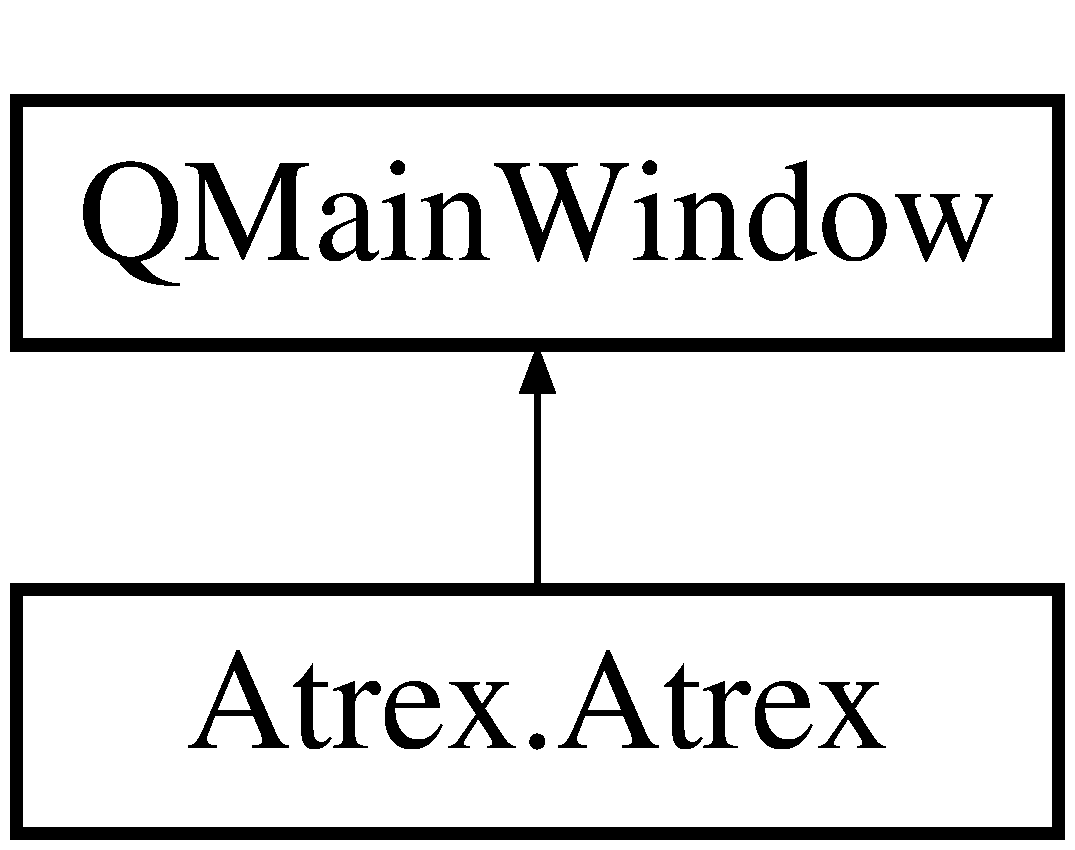
\includegraphics[height=2.000000cm]{classAtrex_1_1Atrex}
\end{center}
\end{figure}
\subsection*{Public Member Functions}
\begin{DoxyCompactItemize}
\item 
def \hyperlink{classAtrex_1_1Atrex_a3c7c6f6088f83b942d6773648e1e6347}{\-\_\-\-\_\-init\-\_\-\-\_\-}
\begin{DoxyCompactList}\small\item\em init -\/ Constructor for the atrex class. \end{DoxyCompactList}\item 
\hypertarget{classAtrex_1_1Atrex_a6877cdfc8717ffc47d5e25a7fa1385f3}{def \hyperlink{classAtrex_1_1Atrex_a6877cdfc8717ffc47d5e25a7fa1385f3}{get\-Home}}\label{classAtrex_1_1Atrex_a6877cdfc8717ffc47d5e25a7fa1385f3}

\begin{DoxyCompactList}\small\item\em get\-Home get the user's home directory \end{DoxyCompactList}\item 
\hypertarget{classAtrex_1_1Atrex_a500ea9d7087f2aaf505f87998d1cf526}{def \hyperlink{classAtrex_1_1Atrex_a500ea9d7087f2aaf505f87998d1cf526}{close\-Event}}\label{classAtrex_1_1Atrex_a500ea9d7087f2aaf505f87998d1cf526}

\begin{DoxyCompactList}\small\item\em close\-Event shut down the program cleanly \end{DoxyCompactList}\item 
\hypertarget{classAtrex_1_1Atrex_aab80061d4d2127e82b592cbf5baef054}{def \hyperlink{classAtrex_1_1Atrex_aab80061d4d2127e82b592cbf5baef054}{open\-Image}}\label{classAtrex_1_1Atrex_aab80061d4d2127e82b592cbf5baef054}

\begin{DoxyCompactList}\small\item\em open\-Image method to open an image, will query the user via an Q\-File\-Dialog \end{DoxyCompactList}\item 
def \hyperlink{classAtrex_1_1Atrex_a25ef435a888471b35045f63fad55b176}{open\-Image\-File}
\begin{DoxyCompactList}\small\item\em open\-Image\-File method to open an image \end{DoxyCompactList}\item 
\hypertarget{classAtrex_1_1Atrex_ab96f78f24269b2608673faa9cec31ad8}{def {\bfseries peak\-Box\-Size\-Set}}\label{classAtrex_1_1Atrex_ab96f78f24269b2608673faa9cec31ad8}

\item 
\hypertarget{classAtrex_1_1Atrex_a02d26a480697d4631d2d8d2c76567a5b}{def {\bfseries zoom\-Fac\-Update}}\label{classAtrex_1_1Atrex_a02d26a480697d4631d2d8d2c76567a5b}

\item 
\hypertarget{classAtrex_1_1Atrex_ab94534c12f07a7fcce69bbfc8a175692}{def {\bfseries new\-Cent}}\label{classAtrex_1_1Atrex_ab94534c12f07a7fcce69bbfc8a175692}

\item 
\hypertarget{classAtrex_1_1Atrex_a3031c6519f2f84e9eee3a482f27132cc}{def {\bfseries new\-Zm\-Box}}\label{classAtrex_1_1Atrex_a3031c6519f2f84e9eee3a482f27132cc}

\item 
\hypertarget{classAtrex_1_1Atrex_a64c7ac662276466211b6d02b2ad9d430}{def {\bfseries disp\-Min\-Pressed}}\label{classAtrex_1_1Atrex_a64c7ac662276466211b6d02b2ad9d430}

\item 
\hypertarget{classAtrex_1_1Atrex_add0fa0a0b9345510d0cf8d834e3734dd}{def {\bfseries disp\-Max\-Pressed}}\label{classAtrex_1_1Atrex_add0fa0a0b9345510d0cf8d834e3734dd}

\item 
\hypertarget{classAtrex_1_1Atrex_a2b706eddbe63823363f801bb0878eb44}{def {\bfseries update\-Image}}\label{classAtrex_1_1Atrex_a2b706eddbe63823363f801bb0878eb44}

\item 
\hypertarget{classAtrex_1_1Atrex_aa8435a0f0357634c9180d2fd4aa5ce75}{def {\bfseries imtype\-Changed}}\label{classAtrex_1_1Atrex_aa8435a0f0357634c9180d2fd4aa5ce75}

\item 
\hypertarget{classAtrex_1_1Atrex_ada591cc2d1c26152ddbaf72f7f7efc4c}{def {\bfseries new\-Slider\-Value}}\label{classAtrex_1_1Atrex_ada591cc2d1c26152ddbaf72f7f7efc4c}

\item 
\hypertarget{classAtrex_1_1Atrex_a9db0c9087a9c3adbb07b2e887322941e}{def {\bfseries decrement\-Image\-Value}}\label{classAtrex_1_1Atrex_a9db0c9087a9c3adbb07b2e887322941e}

\item 
\hypertarget{classAtrex_1_1Atrex_aa766d95d2be1bd5b466da0a2581ca0e5}{def {\bfseries increment\-Image\-Value}}\label{classAtrex_1_1Atrex_aa766d95d2be1bd5b466da0a2581ca0e5}

\item 
\hypertarget{classAtrex_1_1Atrex_acd608751b80f2f6e38b8e3a3c804aba6}{def {\bfseries new\-Image\-Value}}\label{classAtrex_1_1Atrex_acd608751b80f2f6e38b8e3a3c804aba6}

\item 
\hypertarget{classAtrex_1_1Atrex_ae474912922a15f4c46cfa4b81c6428d4}{def {\bfseries max\-Slider\-Update}}\label{classAtrex_1_1Atrex_ae474912922a15f4c46cfa4b81c6428d4}

\item 
\hypertarget{classAtrex_1_1Atrex_ada41f153ca507e3f48294d042e991a79}{def {\bfseries minmax\-D\-N\-Slider\-Released}}\label{classAtrex_1_1Atrex_ada41f153ca507e3f48294d042e991a79}

\item 
\hypertarget{classAtrex_1_1Atrex_aec14907b3f14a48f9805194cd196b67c}{def {\bfseries min\-Slider\-Update}}\label{classAtrex_1_1Atrex_aec14907b3f14a48f9805194cd196b67c}

\item 
\hypertarget{classAtrex_1_1Atrex_aae57dd8400942b0f992b4c4bc868da64}{def {\bfseries lut\-Changed}}\label{classAtrex_1_1Atrex_aae57dd8400942b0f992b4c4bc868da64}

\item 
\hypertarget{classAtrex_1_1Atrex_af3b9d9a660caa590a68da51656d622fb}{def {\bfseries def\-Image\-Dir}}\label{classAtrex_1_1Atrex_af3b9d9a660caa590a68da51656d622fb}

\item 
\hypertarget{classAtrex_1_1Atrex_aca19dbda20686dcaef166d9680528e21}{def {\bfseries def\-Work\-Dir}}\label{classAtrex_1_1Atrex_aca19dbda20686dcaef166d9680528e21}

\item 
\hypertarget{classAtrex_1_1Atrex_ac995f1abf16ed66fea8a907373ff9475}{def {\bfseries image\-Mouse\-Clicked}}\label{classAtrex_1_1Atrex_ac995f1abf16ed66fea8a907373ff9475}

\item 
\hypertarget{classAtrex_1_1Atrex_adc2b173f9b80955c6f4fc7a156e9d091}{def {\bfseries display\-Cake\-Image}}\label{classAtrex_1_1Atrex_adc2b173f9b80955c6f4fc7a156e9d091}

\item 
\hypertarget{classAtrex_1_1Atrex_abfe78ab11ed54f2e83bb9fddfb16a573}{def {\bfseries display\-Image}}\label{classAtrex_1_1Atrex_abfe78ab11ed54f2e83bb9fddfb16a573}

\item 
\hypertarget{classAtrex_1_1Atrex_a101abfd070fc8f268fb07c79026d778e}{def {\bfseries new\-Peak}}\label{classAtrex_1_1Atrex_a101abfd070fc8f268fb07c79026d778e}

\item 
\hypertarget{classAtrex_1_1Atrex_a8778bbe32534eadb568016f2de735ef2}{def {\bfseries update\-Peaks}}\label{classAtrex_1_1Atrex_a8778bbe32534eadb568016f2de735ef2}

\item 
\hypertarget{classAtrex_1_1Atrex_a88cac9434ce28cbff05cb12b81023d4d}{def {\bfseries update\-Peak\-List}}\label{classAtrex_1_1Atrex_a88cac9434ce28cbff05cb12b81023d4d}

\item 
def \hyperlink{classAtrex_1_1Atrex_a2452575598eb0088e452b2160610da4f}{peak\-List\-Clicked}
\begin{DoxyCompactList}\small\item\em peak\-List\-C\-Licked \end{DoxyCompactList}\item 
\hypertarget{classAtrex_1_1Atrex_ace2289de8cacf431113b0a06133c5693}{def {\bfseries adjust\-Peak\-Displays}}\label{classAtrex_1_1Atrex_ace2289de8cacf431113b0a06133c5693}

\item 
\hypertarget{classAtrex_1_1Atrex_a17585a5304b57ea95ad13e6feeebbcde}{def {\bfseries list\-Button\-Changed}}\label{classAtrex_1_1Atrex_a17585a5304b57ea95ad13e6feeebbcde}

\item 
\hypertarget{classAtrex_1_1Atrex_a245293bfb74e32de50e99de66ffeeb55}{def {\bfseries load\-Fit\-Params}}\label{classAtrex_1_1Atrex_a245293bfb74e32de50e99de66ffeeb55}

\item 
\hypertarget{classAtrex_1_1Atrex_a054de9d87526f2849d35862b6747a658}{def {\bfseries zoom\-Mode}}\label{classAtrex_1_1Atrex_a054de9d87526f2849d35862b6747a658}

\item 
\hypertarget{classAtrex_1_1Atrex_a0efd15d4cccf12a54b9263d84dca6d42}{def {\bfseries add\-Peak\-Mode}}\label{classAtrex_1_1Atrex_a0efd15d4cccf12a54b9263d84dca6d42}

\item 
\hypertarget{classAtrex_1_1Atrex_a99248a89609473aaf887150c69e087fd}{def {\bfseries select\-Mode}}\label{classAtrex_1_1Atrex_a99248a89609473aaf887150c69e087fd}

\item 
\hypertarget{classAtrex_1_1Atrex_a739717834e7626d1ba9a1986430f7cf4}{def {\bfseries unselect\-Mode}}\label{classAtrex_1_1Atrex_a739717834e7626d1ba9a1986430f7cf4}

\item 
\hypertarget{classAtrex_1_1Atrex_af107ee890ef60784ad28314a7908c439}{def {\bfseries mask\-Mode}}\label{classAtrex_1_1Atrex_af107ee890ef60784ad28314a7908c439}

\item 
\hypertarget{classAtrex_1_1Atrex_a45a6a72900b8977bc8497f0ad2c0314a}{def {\bfseries unmask\-Mode}}\label{classAtrex_1_1Atrex_a45a6a72900b8977bc8497f0ad2c0314a}

\item 
\hypertarget{classAtrex_1_1Atrex_a96817ca44885b91f7d2ba9cbff61ced5}{def {\bfseries select\-Rect}}\label{classAtrex_1_1Atrex_a96817ca44885b91f7d2ba9cbff61ced5}

\item 
\hypertarget{classAtrex_1_1Atrex_a210da0549837b917dbb10bd194704d67}{def {\bfseries mask\-Rect}}\label{classAtrex_1_1Atrex_a210da0549837b917dbb10bd194704d67}

\item 
\hypertarget{classAtrex_1_1Atrex_a4dce042d175e3f9593319481166886fd}{def {\bfseries clear\-Mask}}\label{classAtrex_1_1Atrex_a4dce042d175e3f9593319481166886fd}

\item 
\hypertarget{classAtrex_1_1Atrex_a9a254e4f37cfc3286bab09e45de45db8}{def {\bfseries save\-Mask}}\label{classAtrex_1_1Atrex_a9a254e4f37cfc3286bab09e45de45db8}

\item 
\hypertarget{classAtrex_1_1Atrex_a3edba6d33e67d7c8cf3eace6aa7bcb1a}{def {\bfseries read\-Mask}}\label{classAtrex_1_1Atrex_a3edba6d33e67d7c8cf3eace6aa7bcb1a}

\item 
\hypertarget{classAtrex_1_1Atrex_ac50dc26f3143315895b9afe212aeaa27}{def {\bfseries sel\-All\-Peaks}}\label{classAtrex_1_1Atrex_ac50dc26f3143315895b9afe212aeaa27}

\item 
\hypertarget{classAtrex_1_1Atrex_aaf655985f170b76903e840bae4cae564}{def {\bfseries clear\-All\-Peaks}}\label{classAtrex_1_1Atrex_aaf655985f170b76903e840bae4cae564}

\item 
\hypertarget{classAtrex_1_1Atrex_a1b95e20242dba81dce9ed56aa33d4502}{def {\bfseries move\-Sel\-Peaks}}\label{classAtrex_1_1Atrex_a1b95e20242dba81dce9ed56aa33d4502}

\item 
\hypertarget{classAtrex_1_1Atrex_ab8dacb09c6a0a632de6bccdc77836dec}{def {\bfseries Remove\-All\-Peaks}}\label{classAtrex_1_1Atrex_ab8dacb09c6a0a632de6bccdc77836dec}

\item 
\hypertarget{classAtrex_1_1Atrex_a3d1ea171a1570456260a8c9e1ff61f2e}{def {\bfseries del\-Sel\-Peaks}}\label{classAtrex_1_1Atrex_a3d1ea171a1570456260a8c9e1ff61f2e}

\item 
\hypertarget{classAtrex_1_1Atrex_a7577e8ee32a4909dde0cdc26cec42439}{def {\bfseries set\-Buttons}}\label{classAtrex_1_1Atrex_a7577e8ee32a4909dde0cdc26cec42439}

\item 
\hypertarget{classAtrex_1_1Atrex_a3ba5414e1ff2fd707ee5aa923371e917}{def {\bfseries update\-Peak\-Number\-L\-E}}\label{classAtrex_1_1Atrex_a3ba5414e1ff2fd707ee5aa923371e917}

\item 
\hypertarget{classAtrex_1_1Atrex_aed5e2cfdb3aa93f0b93f5f92923c10b6}{def {\bfseries open\-Detector\-Calibration}}\label{classAtrex_1_1Atrex_aed5e2cfdb3aa93f0b93f5f92923c10b6}

\item 
\hypertarget{classAtrex_1_1Atrex_a6ddf6ff6c06c18493233eb34db019ac6}{def {\bfseries save\-Detector\-Calibration}}\label{classAtrex_1_1Atrex_a6ddf6ff6c06c18493233eb34db019ac6}

\item 
\hypertarget{classAtrex_1_1Atrex_a33ff7708e43d3f78a0da47e2740b783a}{def {\bfseries Display\-\_\-\-Detector\-\_\-calibration}}\label{classAtrex_1_1Atrex_a33ff7708e43d3f78a0da47e2740b783a}

\item 
\hypertarget{classAtrex_1_1Atrex_abddae09c11c780c9f83fa74a693e3244}{def {\bfseries Update\-\_\-\-Detector\-\_\-calibration}}\label{classAtrex_1_1Atrex_abddae09c11c780c9f83fa74a693e3244}

\item 
\hypertarget{classAtrex_1_1Atrex_a99527243c5cb42e343391bbd921321f0}{def {\bfseries Search\-For\-Peaks}}\label{classAtrex_1_1Atrex_a99527243c5cb42e343391bbd921321f0}

\item 
\hypertarget{classAtrex_1_1Atrex_ad93c17ecc803e8ce3608c80c1e820c9a}{def {\bfseries P\-S}}\label{classAtrex_1_1Atrex_ad93c17ecc803e8ce3608c80c1e820c9a}

\item 
\hypertarget{classAtrex_1_1Atrex_aa44defd7fc02dad7f4371e2a2eccf710}{def {\bfseries Search\-For\-Peaks\-Series}}\label{classAtrex_1_1Atrex_aa44defd7fc02dad7f4371e2a2eccf710}

\item 
\hypertarget{classAtrex_1_1Atrex_a816143e04438e686d80a2172cb484f44}{def {\bfseries merge\-Cancel}}\label{classAtrex_1_1Atrex_a816143e04438e686d80a2172cb484f44}

\item 
\hypertarget{classAtrex_1_1Atrex_acc559ce6fbdf2cb95ada0b191ced0c04}{def {\bfseries merge\-Image\-Range}}\label{classAtrex_1_1Atrex_acc559ce6fbdf2cb95ada0b191ced0c04}

\item 
\hypertarget{classAtrex_1_1Atrex_aff22266d12cc6092353a9e53081edb9d}{def {\bfseries Save\-Peak\-Table}}\label{classAtrex_1_1Atrex_aff22266d12cc6092353a9e53081edb9d}

\item 
\hypertarget{classAtrex_1_1Atrex_af2a8d53b7aa4d5211b9eb3ac25045501}{def {\bfseries Open\-Peak\-Table}}\label{classAtrex_1_1Atrex_af2a8d53b7aa4d5211b9eb3ac25045501}

\item 
\hypertarget{classAtrex_1_1Atrex_aa996a3132c9ace217efe5826349df1df}{def {\bfseries Peak\-List\-Browse}}\label{classAtrex_1_1Atrex_aa996a3132c9ace217efe5826349df1df}

\item 
\hypertarget{classAtrex_1_1Atrex_a5e8c4a39fedb7dff274082c2b7cc352f}{def {\bfseries read\-Text\-Detect}}\label{classAtrex_1_1Atrex_a5e8c4a39fedb7dff274082c2b7cc352f}

\item 
\hypertarget{classAtrex_1_1Atrex_a0545caa06d0d5297147a325e9f2763c5}{def {\bfseries write\-Text\-Detect}}\label{classAtrex_1_1Atrex_a0545caa06d0d5297147a325e9f2763c5}

\item 
\hypertarget{classAtrex_1_1Atrex_ac277ee5f02ff03bf577c91d2351d3833}{def {\bfseries update\-Plot}}\label{classAtrex_1_1Atrex_ac277ee5f02ff03bf577c91d2351d3833}

\item 
\hypertarget{classAtrex_1_1Atrex_a5380dd3e2db37a9e6316dcfb2f79da52}{def {\bfseries save\-Plot\-To\-File}}\label{classAtrex_1_1Atrex_a5380dd3e2db37a9e6316dcfb2f79da52}

\item 
\hypertarget{classAtrex_1_1Atrex_a51c8994be54b7062fd0b7cc077783f52}{def {\bfseries plot\-X\-Y\-From\-File}}\label{classAtrex_1_1Atrex_a51c8994be54b7062fd0b7cc077783f52}

\item 
\hypertarget{classAtrex_1_1Atrex_a4125657b083972e131da1e06587af07f}{def {\bfseries overlay\-Plot\-From\-File}}\label{classAtrex_1_1Atrex_a4125657b083972e131da1e06587af07f}

\item 
\hypertarget{classAtrex_1_1Atrex_a3946e847c41ffc83f4fee8787b1449a7}{def {\bfseries read\-X\-P\-O\-W}}\label{classAtrex_1_1Atrex_a3946e847c41ffc83f4fee8787b1449a7}

\item 
\hypertarget{classAtrex_1_1Atrex_a82e4c50e20fab4518b71703bdde02994}{def {\bfseries read\-J\-C\-P\-D\-S}}\label{classAtrex_1_1Atrex_a82e4c50e20fab4518b71703bdde02994}

\item 
\hypertarget{classAtrex_1_1Atrex_a4a1adbdba785016117f258c281895688}{def {\bfseries int\-Current}}\label{classAtrex_1_1Atrex_a4a1adbdba785016117f258c281895688}

\item 
\hypertarget{classAtrex_1_1Atrex_a4ed5b63695c617a40eb6fc2c50db7575}{def {\bfseries cake\-Current}}\label{classAtrex_1_1Atrex_a4ed5b63695c617a40eb6fc2c50db7575}

\item 
\hypertarget{classAtrex_1_1Atrex_aa1141a78fc819e7fd22a44e1847a89ba}{def {\bfseries test\-Calc}}\label{classAtrex_1_1Atrex_aa1141a78fc819e7fd22a44e1847a89ba}

\item 
\hypertarget{classAtrex_1_1Atrex_ac28031fab9314022a601532483a7b546}{def {\bfseries refine\-Calibration}}\label{classAtrex_1_1Atrex_ac28031fab9314022a601532483a7b546}

\item 
\hypertarget{classAtrex_1_1Atrex_aaa0ad76fcdcdde4e7138ade95031e6c7}{def {\bfseries calc2theta}}\label{classAtrex_1_1Atrex_aaa0ad76fcdcdde4e7138ade95031e6c7}

\item 
\hypertarget{classAtrex_1_1Atrex_ac75d2b26897d6d799773b27b41ea369b}{def {\bfseries done2theta}}\label{classAtrex_1_1Atrex_ac75d2b26897d6d799773b27b41ea369b}

\item 
\hypertarget{classAtrex_1_1Atrex_a4d6871d5055309cbbaddb62e00bfbea5}{def {\bfseries peak\-File\-Browse}}\label{classAtrex_1_1Atrex_a4d6871d5055309cbbaddb62e00bfbea5}

\item 
\hypertarget{classAtrex_1_1Atrex_aaa23b7529d44f3cbbeedfd8434c8bce9}{def {\bfseries peak\-Save\-To\-File}}\label{classAtrex_1_1Atrex_aaa23b7529d44f3cbbeedfd8434c8bce9}

\item 
\hypertarget{classAtrex_1_1Atrex_a3a5f2aee5b962e1615c54395d9edd172}{def \hyperlink{classAtrex_1_1Atrex_a3a5f2aee5b962e1615c54395d9edd172}{plot\-Peak\-Prof}}\label{classAtrex_1_1Atrex_a3a5f2aee5b962e1615c54395d9edd172}

\begin{DoxyCompactList}\small\item\em Function to plot the vertical or horizontal profile of the peak Vert flag controlled by combo-\/box selection This is only for first time, when vbar or hbar is centered on the image. \end{DoxyCompactList}\item 
\hypertarget{classAtrex_1_1Atrex_ad7997e5a735ce1b34d713a4b27490fbc}{def {\bfseries new\-Peak\-Prof\-Location}}\label{classAtrex_1_1Atrex_ad7997e5a735ce1b34d713a4b27490fbc}

\item 
\hypertarget{classAtrex_1_1Atrex_a31041eb876dff6083a13777f44d09274}{def {\bfseries peak\-Prof\-Orientation\-Set}}\label{classAtrex_1_1Atrex_a31041eb876dff6083a13777f44d09274}

\item 
\hypertarget{classAtrex_1_1Atrex_a8ed3b24c6fdcc06364436368a5112f77}{def {\bfseries read\-Predict\-Settings}}\label{classAtrex_1_1Atrex_a8ed3b24c6fdcc06364436368a5112f77}

\item 
\hypertarget{classAtrex_1_1Atrex_a6ec58bcf2c22abf1ad3ac4bf7c9f5db9}{def {\bfseries calibrant\-Changed}}\label{classAtrex_1_1Atrex_a6ec58bcf2c22abf1ad3ac4bf7c9f5db9}

\item 
\hypertarget{classAtrex_1_1Atrex_ad59de2bb679492d17867acb6fffa534e}{def {\bfseries start\-Simulate}}\label{classAtrex_1_1Atrex_ad59de2bb679492d17867acb6fffa534e}

\item 
\hypertarget{classAtrex_1_1Atrex_a9c7db3ee59b336c77f361177d0d14248}{def {\bfseries update\-Display}}\label{classAtrex_1_1Atrex_a9c7db3ee59b336c77f361177d0d14248}

\item 
\hypertarget{classAtrex_1_1Atrex_a74436efac3bb11530dbab592fe41c352}{def {\bfseries read\-\_\-box\-\_\-change}}\label{classAtrex_1_1Atrex_a74436efac3bb11530dbab592fe41c352}

\item 
\hypertarget{classAtrex_1_1Atrex_a8201adc7c4c0956f9adc65b9abdf8172}{def {\bfseries get\-Cal\-Peaks}}\label{classAtrex_1_1Atrex_a8201adc7c4c0956f9adc65b9abdf8172}

\item 
\hypertarget{classAtrex_1_1Atrex_ac8a2db84387587b6d23c8210be13412a}{def {\bfseries read\-\_\-inversions}}\label{classAtrex_1_1Atrex_ac8a2db84387587b6d23c8210be13412a}

\item 
\hypertarget{classAtrex_1_1Atrex_a545132d9586f8d41cb7b4d2637be31db}{def {\bfseries set\-\_\-inversions}}\label{classAtrex_1_1Atrex_a545132d9586f8d41cb7b4d2637be31db}

\item 
\hypertarget{classAtrex_1_1Atrex_a2cefbee9b86a610a4b9b24050808c8fe}{def {\bfseries save\-Proj}}\label{classAtrex_1_1Atrex_a2cefbee9b86a610a4b9b24050808c8fe}

\item 
\hypertarget{classAtrex_1_1Atrex_ab44e996cfacc0e9bd051bd2b91749a63}{def {\bfseries read\-Proj}}\label{classAtrex_1_1Atrex_ab44e996cfacc0e9bd051bd2b91749a63}

\item 
\hypertarget{classAtrex_1_1Atrex_a8e9d3ca6e8e11840ec409b011d3d1b4e}{def {\bfseries load\-\_\-corrections}}\label{classAtrex_1_1Atrex_a8e9d3ca6e8e11840ec409b011d3d1b4e}

\item 
\hypertarget{classAtrex_1_1Atrex_ad9c73604ef72b84b3bfdbf968318db77}{def {\bfseries get\-Omega\-Rotation\-Dir}}\label{classAtrex_1_1Atrex_ad9c73604ef72b84b3bfdbf968318db77}

\item 
\hypertarget{classAtrex_1_1Atrex_a75ea1bb888e8f48f960f4aee73b8a3d0}{def {\bfseries get\-Peak\-Search\-Fit\-Params}}\label{classAtrex_1_1Atrex_a75ea1bb888e8f48f960f4aee73b8a3d0}

\item 
\hypertarget{classAtrex_1_1Atrex_abfc6496a41b59832146a93ad594680eb}{def {\bfseries set\-Val\-To\-Control}}\label{classAtrex_1_1Atrex_abfc6496a41b59832146a93ad594680eb}

\end{DoxyCompactItemize}
\subsection*{Public Attributes}
\begin{DoxyCompactItemize}
\item 
\hypertarget{classAtrex_1_1Atrex_a35cabdfa4a6164da07e19c4b4ed957aa}{{\bfseries ui}}\label{classAtrex_1_1Atrex_a35cabdfa4a6164da07e19c4b4ed957aa}

\item 
\hypertarget{classAtrex_1_1Atrex_aba7d9d2058a5bdace86c305ecd35ad3b}{{\bfseries work\-Directory}}\label{classAtrex_1_1Atrex_aba7d9d2058a5bdace86c305ecd35ad3b}

\item 
\hypertarget{classAtrex_1_1Atrex_a3a5510d39868ddfaae38841e8057394a}{{\bfseries image\-Directory}}\label{classAtrex_1_1Atrex_a3a5510d39868ddfaae38841e8057394a}

\item 
\hypertarget{classAtrex_1_1Atrex_a6c50fb1f9133397ae0936d14310edabd}{{\bfseries image\-File}}\label{classAtrex_1_1Atrex_a6c50fb1f9133397ae0936d14310edabd}

\item 
\hypertarget{classAtrex_1_1Atrex_ac6283b2b56309698f9b3881fd1cb0ba2}{{\bfseries detect\-File}}\label{classAtrex_1_1Atrex_ac6283b2b56309698f9b3881fd1cb0ba2}

\item 
\hypertarget{classAtrex_1_1Atrex_adee5f16f849c0990481863170787811e}{{\bfseries myim}}\label{classAtrex_1_1Atrex_adee5f16f849c0990481863170787811e}

\item 
\hypertarget{classAtrex_1_1Atrex_a7f2c3002d88c2f13aa3f0f19899a0ab7}{{\bfseries zm\-Cent\-Loc}}\label{classAtrex_1_1Atrex_a7f2c3002d88c2f13aa3f0f19899a0ab7}

\item 
\hypertarget{classAtrex_1_1Atrex_a845e289d7ed3657f89da88d1d53657bc}{{\bfseries active\-List}}\label{classAtrex_1_1Atrex_a845e289d7ed3657f89da88d1d53657bc}

\item 
\hypertarget{classAtrex_1_1Atrex_a1fd77da8e55fec3336694f7817bb6cb2}{{\bfseries peaks}}\label{classAtrex_1_1Atrex_a1fd77da8e55fec3336694f7817bb6cb2}

\item 
\hypertarget{classAtrex_1_1Atrex_ad1a660b6c6750e5d21a4c51abffbb2df}{{\bfseries peaks0}}\label{classAtrex_1_1Atrex_ad1a660b6c6750e5d21a4c51abffbb2df}

\item 
\hypertarget{classAtrex_1_1Atrex_ace3b741c1a559e2117246a53d3e8f345}{{\bfseries peaks1}}\label{classAtrex_1_1Atrex_ace3b741c1a559e2117246a53d3e8f345}

\item 
\hypertarget{classAtrex_1_1Atrex_a47354f98e68c5aadcd988d0a2b476889}{{\bfseries detector}}\label{classAtrex_1_1Atrex_a47354f98e68c5aadcd988d0a2b476889}

\item 
\hypertarget{classAtrex_1_1Atrex_a7efc2659254ab5a5f065a5f3fa11ceb9}{\hyperlink{classAtrex_1_1Atrex_a7efc2659254ab5a5f065a5f3fa11ceb9}{fitarr}}\label{classAtrex_1_1Atrex_a7efc2659254ab5a5f065a5f3fa11ceb9}

\begin{DoxyCompactList}\small\item\em .ui.\-zoom\-Tab\-Widgets.\-set\-Current\-Index(0) \end{DoxyCompactList}\item 
\hypertarget{classAtrex_1_1Atrex_a804307169058c96d52235bacc92d6f09}{{\bfseries param\-File}}\label{classAtrex_1_1Atrex_a804307169058c96d52235bacc92d6f09}

\item 
\hypertarget{classAtrex_1_1Atrex_a2080a9ed5c4661217ebd6fa108ef2e68}{{\bfseries base}}\label{classAtrex_1_1Atrex_a2080a9ed5c4661217ebd6fa108ef2e68}

\item 
\hypertarget{classAtrex_1_1Atrex_a8cb32e63ba2e1df2a5819e6df5bfd8e9}{{\bfseries min\-Range}}\label{classAtrex_1_1Atrex_a8cb32e63ba2e1df2a5819e6df5bfd8e9}

\item 
\hypertarget{classAtrex_1_1Atrex_a240f5adcbd64d4282c41fc884722d453}{{\bfseries max\-Range}}\label{classAtrex_1_1Atrex_a240f5adcbd64d4282c41fc884722d453}

\item 
\hypertarget{classAtrex_1_1Atrex_ac181165f963c93be5b4a5e79ac9100e2}{{\bfseries imtype\-Flag}}\label{classAtrex_1_1Atrex_ac181165f963c93be5b4a5e79ac9100e2}

\item 
\hypertarget{classAtrex_1_1Atrex_aaad2acdd3e1ed0343b2414934ce8c257}{\hyperlink{classAtrex_1_1Atrex_aaad2acdd3e1ed0343b2414934ce8c257}{imsize}}\label{classAtrex_1_1Atrex_aaad2acdd3e1ed0343b2414934ce8c257}

\begin{DoxyCompactList}\small\item\em read in the accompanying settings file for the image if it exists \end{DoxyCompactList}\item 
\hypertarget{classAtrex_1_1Atrex_a5a00bf83d75cef3dc64f66b7972128ac}{{\bfseries old\-Selected}}\label{classAtrex_1_1Atrex_a5a00bf83d75cef3dc64f66b7972128ac}

\item 
\hypertarget{classAtrex_1_1Atrex_a9db3f47f57f62dedb23235d73c5b81c7}{{\bfseries peak\-Startx}}\label{classAtrex_1_1Atrex_a9db3f47f57f62dedb23235d73c5b81c7}

\item 
\hypertarget{classAtrex_1_1Atrex_a7128a7471ca115d494fb8457397cb3b4}{{\bfseries peak\-Starty}}\label{classAtrex_1_1Atrex_a7128a7471ca115d494fb8457397cb3b4}

\item 
\hypertarget{classAtrex_1_1Atrex_a9ddce163f1008e4421d95874f8a7e006}{{\bfseries select\-Peak\-X\-Y}}\label{classAtrex_1_1Atrex_a9ddce163f1008e4421d95874f8a7e006}

\item 
\hypertarget{classAtrex_1_1Atrex_a5034cf92d78b203761c82c2d09571fe7}{{\bfseries cancel\-Merge}}\label{classAtrex_1_1Atrex_a5034cf92d78b203761c82c2d09571fe7}

\item 
\hypertarget{classAtrex_1_1Atrex_ac308bffb51e8c4a11b2adbbaf85e38ec}{{\bfseries mysim}}\label{classAtrex_1_1Atrex_ac308bffb51e8c4a11b2adbbaf85e38ec}

\end{DoxyCompactItemize}
\subsection*{Static Public Attributes}
\begin{DoxyCompactItemize}
\item 
\hypertarget{classAtrex_1_1Atrex_adb81a9472392a89ed733d7d0779e45b7}{{\bfseries displayed\-Image} = False}\label{classAtrex_1_1Atrex_adb81a9472392a89ed733d7d0779e45b7}

\item 
\hypertarget{classAtrex_1_1Atrex_ae832c8b0566a3106d3021b88ea739683}{int {\bfseries min\-Range} = 1}\label{classAtrex_1_1Atrex_ae832c8b0566a3106d3021b88ea739683}

\item 
\hypertarget{classAtrex_1_1Atrex_ad050fe0947cfc2aaed121ca1f306d637}{int {\bfseries max\-Range} = 99}\label{classAtrex_1_1Atrex_ad050fe0947cfc2aaed121ca1f306d637}

\item 
\hypertarget{classAtrex_1_1Atrex_a68605f5249c1a23ea96180aa7c011acd}{{\bfseries merge\-Sum\-Mode} = True}\label{classAtrex_1_1Atrex_a68605f5249c1a23ea96180aa7c011acd}

\item 
\hypertarget{classAtrex_1_1Atrex_af008dc7c13f040fea0e0bd315badd461}{tuple {\bfseries mymask} = \hyperlink{classmyMask_1_1myMask}{my\-Mask}()}\label{classAtrex_1_1Atrex_af008dc7c13f040fea0e0bd315badd461}

\item 
\hypertarget{classAtrex_1_1Atrex_af1384190082613188d50f79e7dacb4d4}{tuple {\bfseries mypred} = \hyperlink{classmyPredict_1_1myPredict}{my\-Predict}()}\label{classAtrex_1_1Atrex_af1384190082613188d50f79e7dacb4d4}

\item 
\hypertarget{classAtrex_1_1Atrex_a6c119a7ed751e933a34e165078520474}{string {\bfseries olay\-File} = \char`\"{}\char`\"{}}\label{classAtrex_1_1Atrex_a6c119a7ed751e933a34e165078520474}

\item 
\hypertarget{classAtrex_1_1Atrex_a2ae7c7ded99e983cf654f68a09974198}{{\bfseries olay\-Sec\-Flag} = False}\label{classAtrex_1_1Atrex_a2ae7c7ded99e983cf654f68a09974198}

\item 
\hypertarget{classAtrex_1_1Atrex_a227e61447cc5900a7a818713fffb4d9e}{{\bfseries first\-Display} = True}\label{classAtrex_1_1Atrex_a227e61447cc5900a7a818713fffb4d9e}

\item 
\hypertarget{classAtrex_1_1Atrex_aabc4d80436aab113d3ecabc4fb692c8e}{int {\bfseries imtype\-Flag} = 0}\label{classAtrex_1_1Atrex_aabc4d80436aab113d3ecabc4fb692c8e}

\item 
\hypertarget{classAtrex_1_1Atrex_aec9ff4f8500b49c9d93872db1a458c5e}{list {\bfseries select\-Peak\-X\-Y} = \mbox{[}0.,0.\mbox{]}}\label{classAtrex_1_1Atrex_aec9ff4f8500b49c9d93872db1a458c5e}

\item 
\hypertarget{classAtrex_1_1Atrex_ab1b2d6a17f54b2f004daea4b71512152}{tuple {\bfseries imsize} = (0,0)}\label{classAtrex_1_1Atrex_ab1b2d6a17f54b2f004daea4b71512152}

\item 
\hypertarget{classAtrex_1_1Atrex_a6d1d3398ca810ec9843f350350736793}{int {\bfseries peak\-Box\-Size} = 33}\label{classAtrex_1_1Atrex_a6d1d3398ca810ec9843f350350736793}

\item 
\hypertarget{classAtrex_1_1Atrex_ad74b4f1510f5797e76342de65eaf8433}{int {\bfseries old\-Selected} = -\/1}\label{classAtrex_1_1Atrex_ad74b4f1510f5797e76342de65eaf8433}

\item 
\hypertarget{classAtrex_1_1Atrex_a4ca8a779dc0d0c890538d52bf28dd7da}{{\bfseries vert\-Prof\-Flag} = True}\label{classAtrex_1_1Atrex_a4ca8a779dc0d0c890538d52bf28dd7da}

\item 
\hypertarget{classAtrex_1_1Atrex_a8131137cca435bd72d5a9080f758c0ae}{int {\bfseries peak\-Startx} = 0}\label{classAtrex_1_1Atrex_a8131137cca435bd72d5a9080f758c0ae}

\item 
\hypertarget{classAtrex_1_1Atrex_a52f02e7771533226a5289d5ad149b71e}{int {\bfseries peak\-Starty} = 0}\label{classAtrex_1_1Atrex_a52f02e7771533226a5289d5ad149b71e}

\item 
\hypertarget{classAtrex_1_1Atrex_ac11efcc7aecf0e1378a6ea2403695cd9}{{\bfseries merge\-Arr} = None}\label{classAtrex_1_1Atrex_ac11efcc7aecf0e1378a6ea2403695cd9}

\item 
\hypertarget{classAtrex_1_1Atrex_ab8f629b3d4108ac9fb6bf240b3f08a33}{{\bfseries merge\-File\-Name} = None}\label{classAtrex_1_1Atrex_ab8f629b3d4108ac9fb6bf240b3f08a33}

\item 
\hypertarget{classAtrex_1_1Atrex_a1f1c13bd2ef993ce756a84f7cd7448f7}{{\bfseries merge\-Display\-Flag} = False}\label{classAtrex_1_1Atrex_a1f1c13bd2ef993ce756a84f7cd7448f7}

\item 
\hypertarget{classAtrex_1_1Atrex_a6e11d4a775a3fbcca2fc6cb4f01963eb}{{\bfseries image\-File\-Pref} = None}\label{classAtrex_1_1Atrex_a6e11d4a775a3fbcca2fc6cb4f01963eb}

\item 
\hypertarget{classAtrex_1_1Atrex_a9db69c9f42cd99180c0ce16fab4f4502}{tuple {\bfseries myproj} = \hyperlink{classProject_1_1Project}{Project}()}\label{classAtrex_1_1Atrex_a9db69c9f42cd99180c0ce16fab4f4502}

\end{DoxyCompactItemize}


\subsection{Detailed Description}
\hyperlink{classAtrex_1_1Atrex}{Atrex} Top level class of the \hyperlink{classAtrex_1_1Atrex}{Atrex} software package. 

Loads ui\-Main\-Win.\-ui and handles all events generated by the ui. This is the main control class of the \hyperlink{classAtrex_1_1Atrex}{Atrex} package. 

\subsection{Constructor \& Destructor Documentation}
\hypertarget{classAtrex_1_1Atrex_a3c7c6f6088f83b942d6773648e1e6347}{\index{Atrex\-::\-Atrex@{Atrex\-::\-Atrex}!\-\_\-\-\_\-init\-\_\-\-\_\-@{\-\_\-\-\_\-init\-\_\-\-\_\-}}
\index{\-\_\-\-\_\-init\-\_\-\-\_\-@{\-\_\-\-\_\-init\-\_\-\-\_\-}!Atrex::Atrex@{Atrex\-::\-Atrex}}
\subsubsection[{\-\_\-\-\_\-init\-\_\-\-\_\-}]{\setlength{\rightskip}{0pt plus 5cm}def Atrex.\-Atrex.\-\_\-\-\_\-init\-\_\-\-\_\- (
\begin{DoxyParamCaption}
\item[{}]{self}
\end{DoxyParamCaption}
)}}\label{classAtrex_1_1Atrex_a3c7c6f6088f83b942d6773648e1e6347}


init -\/ Constructor for the atrex class. 

initialize the gui controls, hook signals to slots 

\subsection{Member Function Documentation}
\hypertarget{classAtrex_1_1Atrex_a25ef435a888471b35045f63fad55b176}{\index{Atrex\-::\-Atrex@{Atrex\-::\-Atrex}!open\-Image\-File@{open\-Image\-File}}
\index{open\-Image\-File@{open\-Image\-File}!Atrex::Atrex@{Atrex\-::\-Atrex}}
\subsubsection[{open\-Image\-File}]{\setlength{\rightskip}{0pt plus 5cm}def Atrex.\-Atrex.\-open\-Image\-File (
\begin{DoxyParamCaption}
\item[{}]{self, }
\item[{}]{filename}
\end{DoxyParamCaption}
)}}\label{classAtrex_1_1Atrex_a25ef435a888471b35045f63fad55b176}


open\-Image\-File method to open an image 


\begin{DoxyParams}{Parameters}
{\em filename} & name of file to open from this file the image base will be established. \\
\hline
\end{DoxyParams}
\hypertarget{classAtrex_1_1Atrex_a2452575598eb0088e452b2160610da4f}{\index{Atrex\-::\-Atrex@{Atrex\-::\-Atrex}!peak\-List\-Clicked@{peak\-List\-Clicked}}
\index{peak\-List\-Clicked@{peak\-List\-Clicked}!Atrex::Atrex@{Atrex\-::\-Atrex}}
\subsubsection[{peak\-List\-Clicked}]{\setlength{\rightskip}{0pt plus 5cm}def Atrex.\-Atrex.\-peak\-List\-Clicked (
\begin{DoxyParamCaption}
\item[{}]{self, }
\item[{}]{event}
\end{DoxyParamCaption}
)}}\label{classAtrex_1_1Atrex_a2452575598eb0088e452b2160610da4f}


peak\-List\-C\-Licked 

Define a peak for analysis by clicking the combobox listing all peaks already identified. 

The documentation for this class was generated from the following file\-:\begin{DoxyCompactItemize}
\item 
/home/harold/workdir/atrex/\-Software/Atrex.\-py\end{DoxyCompactItemize}

\hypertarget{structBYTE__STRING}{\section{B\-Y\-T\-E\-\_\-\-S\-T\-R\-I\-N\-G Struct Reference}
\label{structBYTE__STRING}\index{B\-Y\-T\-E\-\_\-\-S\-T\-R\-I\-N\-G@{B\-Y\-T\-E\-\_\-\-S\-T\-R\-I\-N\-G}}
}
\subsection*{Public Attributes}
\begin{DoxyCompactItemize}
\item 
\hypertarget{structBYTE__STRING_a8da8577d70c09a0f8dc481b4d28a7586}{unsigned int {\bfseries ref}}\label{structBYTE__STRING_a8da8577d70c09a0f8dc481b4d28a7586}

\item 
\hypertarget{structBYTE__STRING_a99dbb11de28b137e585323a82ae6d886}{unsigned int {\bfseries len}}\label{structBYTE__STRING_a99dbb11de28b137e585323a82ae6d886}

\item 
\hypertarget{structBYTE__STRING_aa3466d17d921ace130316522aa93b161}{char $\ast$ {\bfseries str}}\label{structBYTE__STRING_aa3466d17d921ace130316522aa93b161}

\end{DoxyCompactItemize}


The documentation for this struct was generated from the following file\-:\begin{DoxyCompactItemize}
\item 
/home/harold/workdir/atrex/\-Software/tifffile.\-c\end{DoxyCompactItemize}

\hypertarget{classcellPathDlg_1_1cellPathDlg}{\section{cell\-Path\-Dlg.\-cell\-Path\-Dlg Class Reference}
\label{classcellPathDlg_1_1cellPathDlg}\index{cell\-Path\-Dlg.\-cell\-Path\-Dlg@{cell\-Path\-Dlg.\-cell\-Path\-Dlg}}
}
Inheritance diagram for cell\-Path\-Dlg.\-cell\-Path\-Dlg\-:\begin{figure}[H]
\begin{center}
\leavevmode
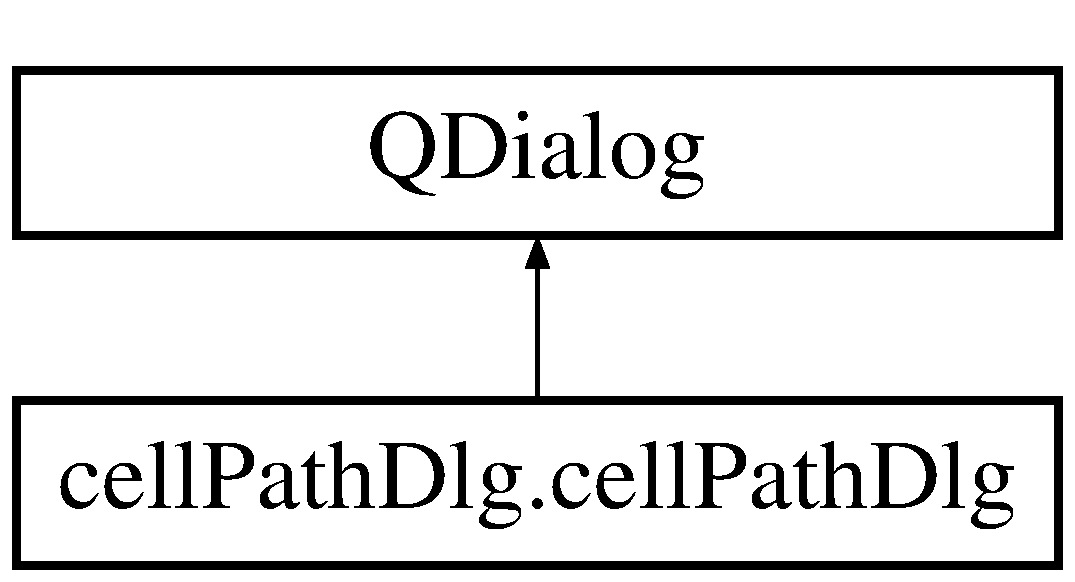
\includegraphics[height=2.000000cm]{classcellPathDlg_1_1cellPathDlg}
\end{center}
\end{figure}
\subsection*{Public Member Functions}
\begin{DoxyCompactItemize}
\item 
\hypertarget{classcellPathDlg_1_1cellPathDlg_aa93992b693c48d47887af3223b221cec}{def {\bfseries \-\_\-\-\_\-init\-\_\-\-\_\-}}\label{classcellPathDlg_1_1cellPathDlg_aa93992b693c48d47887af3223b221cec}

\item 
\hypertarget{classcellPathDlg_1_1cellPathDlg_a13c901781f5bcd4ee0593f0f15345c07}{def \hyperlink{classcellPathDlg_1_1cellPathDlg_a13c901781f5bcd4ee0593f0f15345c07}{browse}}\label{classcellPathDlg_1_1cellPathDlg_a13c901781f5bcd4ee0593f0f15345c07}

\begin{DoxyCompactList}\small\item\em browse for the path to cell\-\_\-now.\-exe \end{DoxyCompactList}\item 
\hypertarget{classcellPathDlg_1_1cellPathDlg_afb506c89586cc5ebc7d4dc91fede7f20}{def {\bfseries ok\-This}}\label{classcellPathDlg_1_1cellPathDlg_afb506c89586cc5ebc7d4dc91fede7f20}

\item 
\hypertarget{classcellPathDlg_1_1cellPathDlg_a15982d7e1a6ee5a1eb0f34482ba037ec}{def {\bfseries cancel\-This}}\label{classcellPathDlg_1_1cellPathDlg_a15982d7e1a6ee5a1eb0f34482ba037ec}

\end{DoxyCompactItemize}
\subsection*{Public Attributes}
\begin{DoxyCompactItemize}
\item 
\hypertarget{classcellPathDlg_1_1cellPathDlg_af004a0758946e90d601ec2180453c60a}{{\bfseries ui}}\label{classcellPathDlg_1_1cellPathDlg_af004a0758946e90d601ec2180453c60a}

\item 
\hypertarget{classcellPathDlg_1_1cellPathDlg_a0a857af36f6583033648fb23a8369c00}{{\bfseries path}}\label{classcellPathDlg_1_1cellPathDlg_a0a857af36f6583033648fb23a8369c00}

\item 
\hypertarget{classcellPathDlg_1_1cellPathDlg_adf6303625eb528b1432bf7913b2866ee}{{\bfseries status}}\label{classcellPathDlg_1_1cellPathDlg_adf6303625eb528b1432bf7913b2866ee}

\end{DoxyCompactItemize}


The documentation for this class was generated from the following file\-:\begin{DoxyCompactItemize}
\item 
/home/harold/workdir/atrex/\-Software/cell\-Path\-Dlg.\-py\end{DoxyCompactItemize}

\hypertarget{classtifffile_1_1TiffTag_1_1Error}{\section{tifffile.\-Tiff\-Tag.\-Error Class Reference}
\label{classtifffile_1_1TiffTag_1_1Error}\index{tifffile.\-Tiff\-Tag.\-Error@{tifffile.\-Tiff\-Tag.\-Error}}
}
Inheritance diagram for tifffile.\-Tiff\-Tag.\-Error\-:\begin{figure}[H]
\begin{center}
\leavevmode
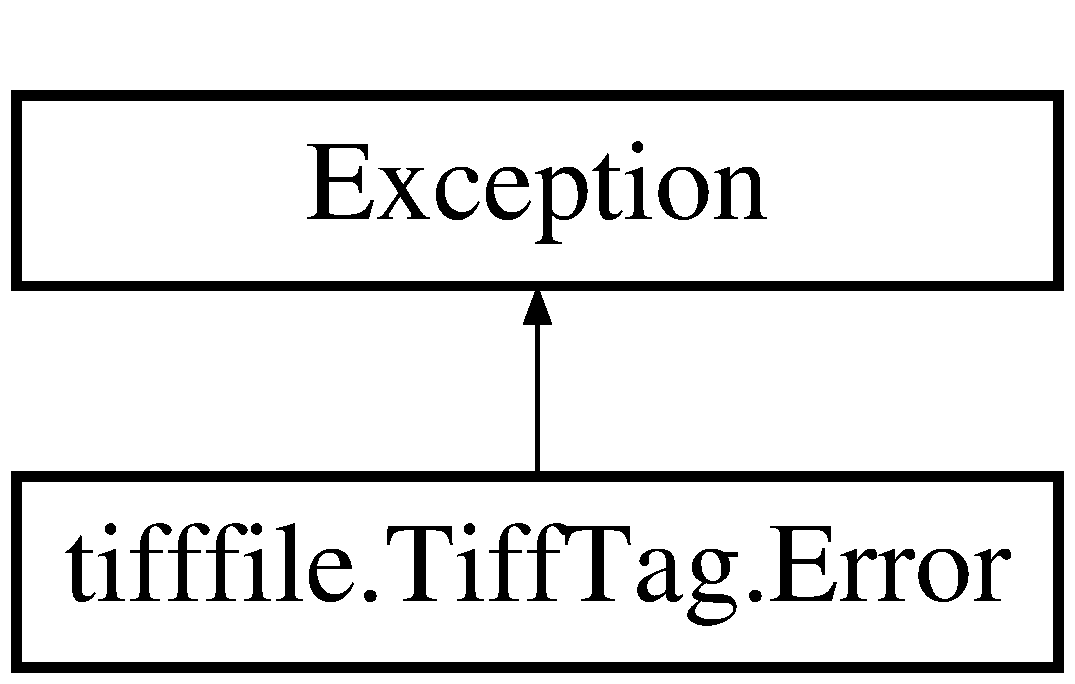
\includegraphics[height=2.000000cm]{classtifffile_1_1TiffTag_1_1Error}
\end{center}
\end{figure}


The documentation for this class was generated from the following file\-:\begin{DoxyCompactItemize}
\item 
/home/harold/workdir/atrex/\-Software/tifffile.\-py\end{DoxyCompactItemize}

\hypertarget{classtifffile_1_1FileHandle}{\section{tifffile.\-File\-Handle Class Reference}
\label{classtifffile_1_1FileHandle}\index{tifffile.\-File\-Handle@{tifffile.\-File\-Handle}}
}
Inheritance diagram for tifffile.\-File\-Handle\-:\begin{figure}[H]
\begin{center}
\leavevmode
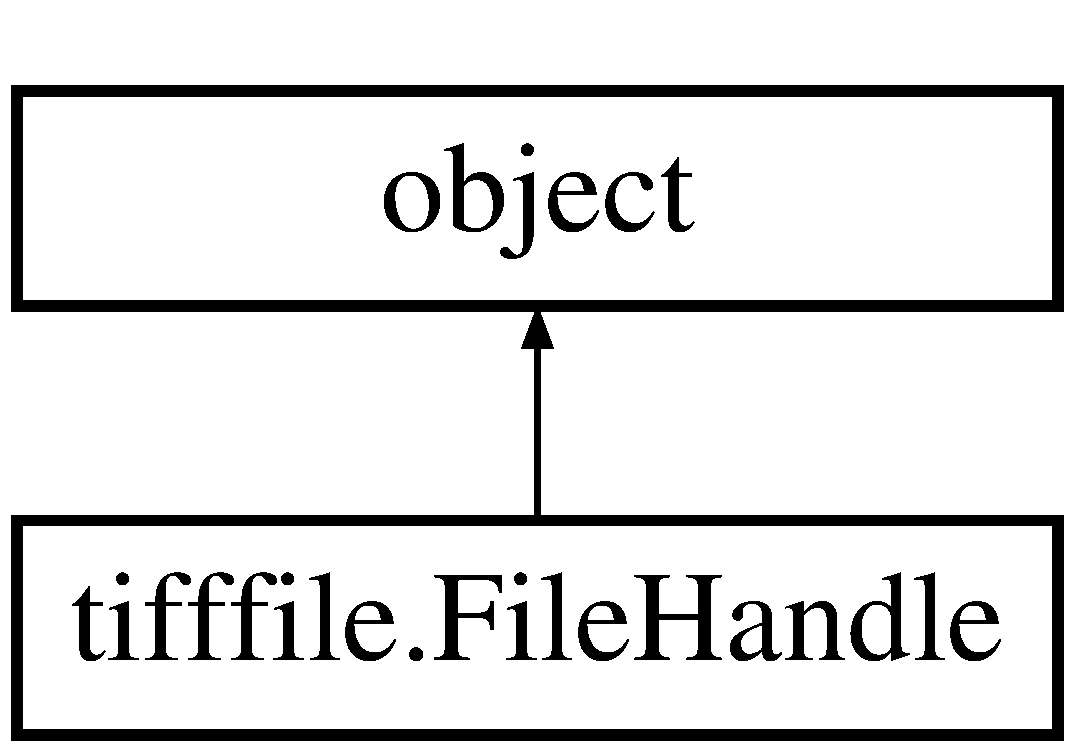
\includegraphics[height=2.000000cm]{classtifffile_1_1FileHandle}
\end{center}
\end{figure}
\subsection*{Public Member Functions}
\begin{DoxyCompactItemize}
\item 
def \hyperlink{classtifffile_1_1FileHandle_a256d28d56fa26bdc5a54056626dba06b}{\-\_\-\-\_\-init\-\_\-\-\_\-}
\item 
def \hyperlink{classtifffile_1_1FileHandle_aed5fb2120f32ee43f63a74e51ee19014}{open}
\item 
def \hyperlink{classtifffile_1_1FileHandle_a11284915485b77b0666fab6c13ff3052}{read}
\item 
def \hyperlink{classtifffile_1_1FileHandle_a57407ec5af06d23c9bad8c8b94a4c1e4}{memmap\-\_\-array}
\item 
def \hyperlink{classtifffile_1_1FileHandle_ae9a3b8d51a50d9cac82f80a33e3c9887}{read\-\_\-array}
\item 
def \hyperlink{classtifffile_1_1FileHandle_ace4a33bbf8c889940fea17f043042ce3}{read\-\_\-record}
\item 
def \hyperlink{classtifffile_1_1FileHandle_ac6a2ba4f361ef961cb206c2199513c70}{tell}
\item 
def \hyperlink{classtifffile_1_1FileHandle_a88d4b64db22c7a55afae0428b5e0200a}{seek}
\item 
def \hyperlink{classtifffile_1_1FileHandle_a8c345933b2368352aa97ee72aaeda596}{close}
\item 
\hypertarget{classtifffile_1_1FileHandle_af0dcfc3f144e9ab96946cf8063142574}{def {\bfseries \-\_\-\-\_\-enter\-\_\-\-\_\-}}\label{classtifffile_1_1FileHandle_af0dcfc3f144e9ab96946cf8063142574}

\item 
\hypertarget{classtifffile_1_1FileHandle_a7a59eb04f16fee7fafead1200bb4871b}{def {\bfseries \-\_\-\-\_\-exit\-\_\-\-\_\-}}\label{classtifffile_1_1FileHandle_a7a59eb04f16fee7fafead1200bb4871b}

\item 
def \hyperlink{classtifffile_1_1FileHandle_a4ab2bf69b0a273e2ee43db2d9f2536b5}{\-\_\-\-\_\-getattr\-\_\-\-\_\-}
\item 
\hypertarget{classtifffile_1_1FileHandle_a65426db83982602cb1e3e301eddf9fd6}{def {\bfseries name}}\label{classtifffile_1_1FileHandle_a65426db83982602cb1e3e301eddf9fd6}

\item 
\hypertarget{classtifffile_1_1FileHandle_a1816f4d0d7568ebb37e4b473e527e106}{def {\bfseries dirname}}\label{classtifffile_1_1FileHandle_a1816f4d0d7568ebb37e4b473e527e106}

\item 
\hypertarget{classtifffile_1_1FileHandle_a23b95cb72e478e26496e6d3d7527a3a3}{def {\bfseries path}}\label{classtifffile_1_1FileHandle_a23b95cb72e478e26496e6d3d7527a3a3}

\item 
\hypertarget{classtifffile_1_1FileHandle_a8fc096aaf40c918ccfc6f61304c63384}{def {\bfseries size}}\label{classtifffile_1_1FileHandle_a8fc096aaf40c918ccfc6f61304c63384}

\item 
\hypertarget{classtifffile_1_1FileHandle_ac35c2f69232e3c539f7b5859db1239c4}{def {\bfseries closed}}\label{classtifffile_1_1FileHandle_ac35c2f69232e3c539f7b5859db1239c4}

\end{DoxyCompactItemize}
\subsection*{Public Attributes}
\begin{DoxyCompactItemize}
\item 
\hypertarget{classtifffile_1_1FileHandle_a965cb7fae14d9f259b2197072da2cf2e}{{\bfseries is\-\_\-file}}\label{classtifffile_1_1FileHandle_a965cb7fae14d9f259b2197072da2cf2e}

\end{DoxyCompactItemize}


\subsection{Detailed Description}
\begin{DoxyVerb}Binary file handle.

* Handle embedded files (for CZI within CZI files).
* Allow to re-open closed files (for multi file formats such as OME-TIFF).
* Read numpy arrays and records from file like objects.

Only binary read, seek, tell, and close are supported on embedded files.
When initialized from another file handle, do not use it unless this
FileHandle is closed.

Attributes
----------
name : str
    Name of the file.
path : str
    Absolute path to file.
size : int
    Size of file in bytes.
is_file : bool
    If True, file has a filno and can be memory mapped.

All attributes are read-only.\end{DoxyVerb}
 

\subsection{Constructor \& Destructor Documentation}
\hypertarget{classtifffile_1_1FileHandle_a256d28d56fa26bdc5a54056626dba06b}{\index{tifffile\-::\-File\-Handle@{tifffile\-::\-File\-Handle}!\-\_\-\-\_\-init\-\_\-\-\_\-@{\-\_\-\-\_\-init\-\_\-\-\_\-}}
\index{\-\_\-\-\_\-init\-\_\-\-\_\-@{\-\_\-\-\_\-init\-\_\-\-\_\-}!tifffile::FileHandle@{tifffile\-::\-File\-Handle}}
\subsubsection[{\-\_\-\-\_\-init\-\_\-\-\_\-}]{\setlength{\rightskip}{0pt plus 5cm}def tifffile.\-File\-Handle.\-\_\-\-\_\-init\-\_\-\-\_\- (
\begin{DoxyParamCaption}
\item[{}]{self, }
\item[{}]{arg, }
\item[{}]{mode = {\ttfamily 'rb'}, }
\item[{}]{name = {\ttfamily None}, }
\item[{}]{offset = {\ttfamily None}, }
\item[{}]{size = {\ttfamily None}}
\end{DoxyParamCaption}
)}}\label{classtifffile_1_1FileHandle_a256d28d56fa26bdc5a54056626dba06b}
\begin{DoxyVerb}Initialize file handle from file name or another file handle.

Parameters
----------
arg : str, File, or FileHandle
    File name or open file handle.
mode : str
    File open mode in case 'arg' is a file name.
name : str
    Optional name of file in case 'arg' is a file handle.
offset : int
    Optional start position of embedded file. By default this is
    the current file position.
size : int
    Optional size of embedded file. By default this is the number
    of bytes from the 'offset' to the end of the file.\end{DoxyVerb}
 

\subsection{Member Function Documentation}
\hypertarget{classtifffile_1_1FileHandle_a4ab2bf69b0a273e2ee43db2d9f2536b5}{\index{tifffile\-::\-File\-Handle@{tifffile\-::\-File\-Handle}!\-\_\-\-\_\-getattr\-\_\-\-\_\-@{\-\_\-\-\_\-getattr\-\_\-\-\_\-}}
\index{\-\_\-\-\_\-getattr\-\_\-\-\_\-@{\-\_\-\-\_\-getattr\-\_\-\-\_\-}!tifffile::FileHandle@{tifffile\-::\-File\-Handle}}
\subsubsection[{\-\_\-\-\_\-getattr\-\_\-\-\_\-}]{\setlength{\rightskip}{0pt plus 5cm}def tifffile.\-File\-Handle.\-\_\-\-\_\-getattr\-\_\-\-\_\- (
\begin{DoxyParamCaption}
\item[{}]{self, }
\item[{}]{name}
\end{DoxyParamCaption}
)}}\label{classtifffile_1_1FileHandle_a4ab2bf69b0a273e2ee43db2d9f2536b5}
\begin{DoxyVerb}Return attribute from underlying file object.\end{DoxyVerb}
 \hypertarget{classtifffile_1_1FileHandle_a8c345933b2368352aa97ee72aaeda596}{\index{tifffile\-::\-File\-Handle@{tifffile\-::\-File\-Handle}!close@{close}}
\index{close@{close}!tifffile::FileHandle@{tifffile\-::\-File\-Handle}}
\subsubsection[{close}]{\setlength{\rightskip}{0pt plus 5cm}def tifffile.\-File\-Handle.\-close (
\begin{DoxyParamCaption}
\item[{}]{self}
\end{DoxyParamCaption}
)}}\label{classtifffile_1_1FileHandle_a8c345933b2368352aa97ee72aaeda596}
\begin{DoxyVerb}Close file.\end{DoxyVerb}
 \hypertarget{classtifffile_1_1FileHandle_a57407ec5af06d23c9bad8c8b94a4c1e4}{\index{tifffile\-::\-File\-Handle@{tifffile\-::\-File\-Handle}!memmap\-\_\-array@{memmap\-\_\-array}}
\index{memmap\-\_\-array@{memmap\-\_\-array}!tifffile::FileHandle@{tifffile\-::\-File\-Handle}}
\subsubsection[{memmap\-\_\-array}]{\setlength{\rightskip}{0pt plus 5cm}def tifffile.\-File\-Handle.\-memmap\-\_\-array (
\begin{DoxyParamCaption}
\item[{}]{self, }
\item[{}]{dtype, }
\item[{}]{shape, }
\item[{}]{offset = {\ttfamily 0}, }
\item[{}]{mode = {\ttfamily 'r'}, }
\item[{}]{order = {\ttfamily 'C'}}
\end{DoxyParamCaption}
)}}\label{classtifffile_1_1FileHandle_a57407ec5af06d23c9bad8c8b94a4c1e4}
\begin{DoxyVerb}Return numpy.memmap of data stored in file.\end{DoxyVerb}
 \hypertarget{classtifffile_1_1FileHandle_aed5fb2120f32ee43f63a74e51ee19014}{\index{tifffile\-::\-File\-Handle@{tifffile\-::\-File\-Handle}!open@{open}}
\index{open@{open}!tifffile::FileHandle@{tifffile\-::\-File\-Handle}}
\subsubsection[{open}]{\setlength{\rightskip}{0pt plus 5cm}def tifffile.\-File\-Handle.\-open (
\begin{DoxyParamCaption}
\item[{}]{self}
\end{DoxyParamCaption}
)}}\label{classtifffile_1_1FileHandle_aed5fb2120f32ee43f63a74e51ee19014}
\begin{DoxyVerb}Open or re-open file.\end{DoxyVerb}
 \hypertarget{classtifffile_1_1FileHandle_a11284915485b77b0666fab6c13ff3052}{\index{tifffile\-::\-File\-Handle@{tifffile\-::\-File\-Handle}!read@{read}}
\index{read@{read}!tifffile::FileHandle@{tifffile\-::\-File\-Handle}}
\subsubsection[{read}]{\setlength{\rightskip}{0pt plus 5cm}def tifffile.\-File\-Handle.\-read (
\begin{DoxyParamCaption}
\item[{}]{self, }
\item[{}]{size = {\ttfamily -\/1}}
\end{DoxyParamCaption}
)}}\label{classtifffile_1_1FileHandle_a11284915485b77b0666fab6c13ff3052}
\begin{DoxyVerb}Read 'size' bytes from file, or until EOF is reached.\end{DoxyVerb}
 \hypertarget{classtifffile_1_1FileHandle_ae9a3b8d51a50d9cac82f80a33e3c9887}{\index{tifffile\-::\-File\-Handle@{tifffile\-::\-File\-Handle}!read\-\_\-array@{read\-\_\-array}}
\index{read\-\_\-array@{read\-\_\-array}!tifffile::FileHandle@{tifffile\-::\-File\-Handle}}
\subsubsection[{read\-\_\-array}]{\setlength{\rightskip}{0pt plus 5cm}def tifffile.\-File\-Handle.\-read\-\_\-array (
\begin{DoxyParamCaption}
\item[{}]{self, }
\item[{}]{dtype, }
\item[{}]{count = {\ttfamily -\/1}, }
\item[{}]{sep = {\ttfamily \char`\"{}\char`\"{}}}
\end{DoxyParamCaption}
)}}\label{classtifffile_1_1FileHandle_ae9a3b8d51a50d9cac82f80a33e3c9887}
\begin{DoxyVerb}Return numpy array from file.

Work around numpy issue #2230, "numpy.fromfile does not accept
StringIO object" https://github.com/numpy/numpy/issues/2230.\end{DoxyVerb}
 \hypertarget{classtifffile_1_1FileHandle_ace4a33bbf8c889940fea17f043042ce3}{\index{tifffile\-::\-File\-Handle@{tifffile\-::\-File\-Handle}!read\-\_\-record@{read\-\_\-record}}
\index{read\-\_\-record@{read\-\_\-record}!tifffile::FileHandle@{tifffile\-::\-File\-Handle}}
\subsubsection[{read\-\_\-record}]{\setlength{\rightskip}{0pt plus 5cm}def tifffile.\-File\-Handle.\-read\-\_\-record (
\begin{DoxyParamCaption}
\item[{}]{self, }
\item[{}]{dtype, }
\item[{}]{shape = {\ttfamily 1}, }
\item[{}]{byteorder = {\ttfamily None}}
\end{DoxyParamCaption}
)}}\label{classtifffile_1_1FileHandle_ace4a33bbf8c889940fea17f043042ce3}
\begin{DoxyVerb}Return numpy record from file.\end{DoxyVerb}
 \hypertarget{classtifffile_1_1FileHandle_a88d4b64db22c7a55afae0428b5e0200a}{\index{tifffile\-::\-File\-Handle@{tifffile\-::\-File\-Handle}!seek@{seek}}
\index{seek@{seek}!tifffile::FileHandle@{tifffile\-::\-File\-Handle}}
\subsubsection[{seek}]{\setlength{\rightskip}{0pt plus 5cm}def tifffile.\-File\-Handle.\-seek (
\begin{DoxyParamCaption}
\item[{}]{self, }
\item[{}]{offset, }
\item[{}]{whence = {\ttfamily 0}}
\end{DoxyParamCaption}
)}}\label{classtifffile_1_1FileHandle_a88d4b64db22c7a55afae0428b5e0200a}
\begin{DoxyVerb}Set file's current position.\end{DoxyVerb}
 \hypertarget{classtifffile_1_1FileHandle_ac6a2ba4f361ef961cb206c2199513c70}{\index{tifffile\-::\-File\-Handle@{tifffile\-::\-File\-Handle}!tell@{tell}}
\index{tell@{tell}!tifffile::FileHandle@{tifffile\-::\-File\-Handle}}
\subsubsection[{tell}]{\setlength{\rightskip}{0pt plus 5cm}def tifffile.\-File\-Handle.\-tell (
\begin{DoxyParamCaption}
\item[{}]{self}
\end{DoxyParamCaption}
)}}\label{classtifffile_1_1FileHandle_ac6a2ba4f361ef961cb206c2199513c70}
\begin{DoxyVerb}Return file's current position.\end{DoxyVerb}
 

The documentation for this class was generated from the following file\-:\begin{DoxyCompactItemize}
\item 
/home/harold/workdir/atrex/\-Software/tifffile.\-py\end{DoxyCompactItemize}

\hypertarget{classJCPDS_1_1JCPDS}{\section{J\-C\-P\-D\-S.\-J\-C\-P\-D\-S Class Reference}
\label{classJCPDS_1_1JCPDS}\index{J\-C\-P\-D\-S.\-J\-C\-P\-D\-S@{J\-C\-P\-D\-S.\-J\-C\-P\-D\-S}}
}
\subsection*{Public Member Functions}
\begin{DoxyCompactItemize}
\item 
\hypertarget{classJCPDS_1_1JCPDS_aca0207da67855730a22a3bbcd031c1d3}{def {\bfseries \-\_\-\-\_\-init\-\_\-\-\_\-}}\label{classJCPDS_1_1JCPDS_aca0207da67855730a22a3bbcd031c1d3}

\item 
\hypertarget{classJCPDS_1_1JCPDS_ab3335931a8dbbff1bff32de39d752723}{def {\bfseries read\-\_\-file}}\label{classJCPDS_1_1JCPDS_ab3335931a8dbbff1bff32de39d752723}

\item 
\hypertarget{classJCPDS_1_1JCPDS_a728290518d30c0c2df73cf1383515768}{def {\bfseries read\-\_\-xpow}}\label{classJCPDS_1_1JCPDS_a728290518d30c0c2df73cf1383515768}

\item 
\hypertarget{classJCPDS_1_1JCPDS_a229ed071c04b6cb367ea7b349539e711}{def {\bfseries write\-\_\-file}}\label{classJCPDS_1_1JCPDS_a229ed071c04b6cb367ea7b349539e711}

\item 
\hypertarget{classJCPDS_1_1JCPDS_a9bce7cbc5045239ca4175d750256e6aa}{def {\bfseries compute\-\_\-\-D}}\label{classJCPDS_1_1JCPDS_a9bce7cbc5045239ca4175d750256e6aa}

\item 
\hypertarget{classJCPDS_1_1JCPDS_a3d9ee706776a7e24826e8a21ac8ac51a}{def {\bfseries compute\-\_\-v0}}\label{classJCPDS_1_1JCPDS_a3d9ee706776a7e24826e8a21ac8ac51a}

\item 
\hypertarget{classJCPDS_1_1JCPDS_a15973313ee7187e0e0bef03b1aebed0e}{def {\bfseries compute\-\_\-v}}\label{classJCPDS_1_1JCPDS_a15973313ee7187e0e0bef03b1aebed0e}

\item 
\hypertarget{classJCPDS_1_1JCPDS_aa837bef35e9c46e89a6c2673dfaa10b8}{def {\bfseries compute\-\_\-volume}}\label{classJCPDS_1_1JCPDS_aa837bef35e9c46e89a6c2673dfaa10b8}

\item 
\hypertarget{classJCPDS_1_1JCPDS_ad256df2c1ea42c6ed31ff86bb577981a}{def {\bfseries bm3\-\_\-pressure}}\label{classJCPDS_1_1JCPDS_ad256df2c1ea42c6ed31ff86bb577981a}

\item 
\hypertarget{classJCPDS_1_1JCPDS_a73e3fb2c332bde54412906eaf49b5693}{def {\bfseries check\-\_\-for\-\_\-equivalents}}\label{classJCPDS_1_1JCPDS_a73e3fb2c332bde54412906eaf49b5693}

\item 
\hypertarget{classJCPDS_1_1JCPDS_acd0737c833865f0efd2b3e8dd273c909}{def {\bfseries copy\-\_\-object1}}\label{classJCPDS_1_1JCPDS_acd0737c833865f0efd2b3e8dd273c909}

\item 
\hypertarget{classJCPDS_1_1JCPDS_a3ce0c985ae5d2016ace2766ca2f520ee}{def {\bfseries copy\-\_\-object}}\label{classJCPDS_1_1JCPDS_a3ce0c985ae5d2016ace2766ca2f520ee}

\item 
\hypertarget{classJCPDS_1_1JCPDS_aa3b28978840f14b05fa13d88d083b214}{def {\bfseries generate\-\_\-accessible\-\_\-peaks}}\label{classJCPDS_1_1JCPDS_aa3b28978840f14b05fa13d88d083b214}

\item 
\hypertarget{classJCPDS_1_1JCPDS_a32a90e34a4d32069f00a6f6537dc91dc}{def {\bfseries get\-\_\-ks}}\label{classJCPDS_1_1JCPDS_a32a90e34a4d32069f00a6f6537dc91dc}

\item 
\hypertarget{classJCPDS_1_1JCPDS_a36e77efd2364a3f81ef463ffb959d07e}{def {\bfseries set\-\_\-ks}}\label{classJCPDS_1_1JCPDS_a36e77efd2364a3f81ef463ffb959d07e}

\item 
\hypertarget{classJCPDS_1_1JCPDS_a06b183ba8881c7197a063b860083dfd8}{def {\bfseries get\-\_\-lp}}\label{classJCPDS_1_1JCPDS_a06b183ba8881c7197a063b860083dfd8}

\item 
\hypertarget{classJCPDS_1_1JCPDS_aabe3f59ba92dfb4712082c77d74a28b0}{def {\bfseries get\-\_\-lp0}}\label{classJCPDS_1_1JCPDS_aabe3f59ba92dfb4712082c77d74a28b0}

\item 
\hypertarget{classJCPDS_1_1JCPDS_a957b63b325687580b686ea88741fdfb8}{def {\bfseries calculate\-\_\-abc}}\label{classJCPDS_1_1JCPDS_a957b63b325687580b686ea88741fdfb8}

\item 
\hypertarget{classJCPDS_1_1JCPDS_aaf4441ec7e191848281e381982568c74}{def {\bfseries set\-\_\-lp}}\label{classJCPDS_1_1JCPDS_aaf4441ec7e191848281e381982568c74}

\item 
\hypertarget{classJCPDS_1_1JCPDS_abe8101e5474e729f2d067fcc61561a31}{def {\bfseries set\-\_\-lp0}}\label{classJCPDS_1_1JCPDS_abe8101e5474e729f2d067fcc61561a31}

\item 
\hypertarget{classJCPDS_1_1JCPDS_a92e518955551c7e65dad79bb40d5181a}{def {\bfseries get\-\_\-symmetry}}\label{classJCPDS_1_1JCPDS_a92e518955551c7e65dad79bb40d5181a}

\item 
\hypertarget{classJCPDS_1_1JCPDS_a8cd753161864e176f79874f9ee55ca9b}{def {\bfseries set\-\_\-symmetry}}\label{classJCPDS_1_1JCPDS_a8cd753161864e176f79874f9ee55ca9b}

\item 
\hypertarget{classJCPDS_1_1JCPDS_ab2c9774755de8f1b98fbd75fca00281e}{def {\bfseries set\-\_\-comment}}\label{classJCPDS_1_1JCPDS_ab2c9774755de8f1b98fbd75fca00281e}

\item 
\hypertarget{classJCPDS_1_1JCPDS_ab93dd1b1d99684d5ee51713afc042413}{def {\bfseries get\-\_\-comment}}\label{classJCPDS_1_1JCPDS_ab93dd1b1d99684d5ee51713afc042413}

\item 
\hypertarget{classJCPDS_1_1JCPDS_adf2e6b325f00594a550653a6a150215d}{def {\bfseries set\-\_\-reflections}}\label{classJCPDS_1_1JCPDS_adf2e6b325f00594a550653a6a150215d}

\item 
\hypertarget{classJCPDS_1_1JCPDS_a125df1699b3e7f91e14e19c7035152e9}{def {\bfseries get\-\_\-reflections\-\_\-\-P\-C}}\label{classJCPDS_1_1JCPDS_a125df1699b3e7f91e14e19c7035152e9}

\item 
\hypertarget{classJCPDS_1_1JCPDS_a1d48c932a6349263167926e057807c3f}{def {\bfseries get\-Param\-String}}\label{classJCPDS_1_1JCPDS_a1d48c932a6349263167926e057807c3f}

\end{DoxyCompactItemize}
\subsection*{Public Attributes}
\begin{DoxyCompactItemize}
\item 
\hypertarget{classJCPDS_1_1JCPDS_a809397a9da7c35ae0a3ad9fca1cabc73}{{\bfseries a}}\label{classJCPDS_1_1JCPDS_a809397a9da7c35ae0a3ad9fca1cabc73}

\item 
\hypertarget{classJCPDS_1_1JCPDS_af32006e867dad5c863a396af1590c34f}{{\bfseries version}}\label{classJCPDS_1_1JCPDS_af32006e867dad5c863a396af1590c34f}

\item 
\hypertarget{classJCPDS_1_1JCPDS_ac7bb249be2c2ff3d89ca89c5cf9fba26}{{\bfseries filename}}\label{classJCPDS_1_1JCPDS_ac7bb249be2c2ff3d89ca89c5cf9fba26}

\item 
\hypertarget{classJCPDS_1_1JCPDS_a5107a25f1f6940a39ce5f7391ff87b21}{{\bfseries k0}}\label{classJCPDS_1_1JCPDS_a5107a25f1f6940a39ce5f7391ff87b21}

\item 
\hypertarget{classJCPDS_1_1JCPDS_a20801fc810dd360855e81c7c8c486d78}{{\bfseries k0p}}\label{classJCPDS_1_1JCPDS_a20801fc810dd360855e81c7c8c486d78}

\item 
\hypertarget{classJCPDS_1_1JCPDS_a1423572b84a46fa0739fba9892d55fdf}{{\bfseries dk0dt}}\label{classJCPDS_1_1JCPDS_a1423572b84a46fa0739fba9892d55fdf}

\item 
\hypertarget{classJCPDS_1_1JCPDS_a281da0716f471977727858228cbddaa4}{{\bfseries dk0pdt}}\label{classJCPDS_1_1JCPDS_a281da0716f471977727858228cbddaa4}

\item 
\hypertarget{classJCPDS_1_1JCPDS_af8dfc3bb57b6bd48b9eeed7d4eb19685}{{\bfseries symmetry}}\label{classJCPDS_1_1JCPDS_af8dfc3bb57b6bd48b9eeed7d4eb19685}

\item 
\hypertarget{classJCPDS_1_1JCPDS_acfb0a8fef740164e10c7b87d92aa82d6}{{\bfseries a0}}\label{classJCPDS_1_1JCPDS_acfb0a8fef740164e10c7b87d92aa82d6}

\item 
\hypertarget{classJCPDS_1_1JCPDS_a7760bcfe96b190ba393928e70ed996cb}{{\bfseries b0}}\label{classJCPDS_1_1JCPDS_a7760bcfe96b190ba393928e70ed996cb}

\item 
\hypertarget{classJCPDS_1_1JCPDS_a81fa032e6345e4ec9baa962f65507ef6}{{\bfseries c0}}\label{classJCPDS_1_1JCPDS_a81fa032e6345e4ec9baa962f65507ef6}

\item 
\hypertarget{classJCPDS_1_1JCPDS_a8b17a58f7870b085673c881db21b8335}{{\bfseries alpha0}}\label{classJCPDS_1_1JCPDS_a8b17a58f7870b085673c881db21b8335}

\item 
\hypertarget{classJCPDS_1_1JCPDS_a45086584379c67ece36240b890741c61}{{\bfseries beta0}}\label{classJCPDS_1_1JCPDS_a45086584379c67ece36240b890741c61}

\item 
\hypertarget{classJCPDS_1_1JCPDS_aa9826897893cdc97c509c90187c61d8c}{{\bfseries gamma0}}\label{classJCPDS_1_1JCPDS_aa9826897893cdc97c509c90187c61d8c}

\item 
\hypertarget{classJCPDS_1_1JCPDS_aef3a4e5b9b3659dc953d276e53a12743}{{\bfseries v0}}\label{classJCPDS_1_1JCPDS_aef3a4e5b9b3659dc953d276e53a12743}

\item 
\hypertarget{classJCPDS_1_1JCPDS_ae09f3ff37073046c2ceb1c1aa3a6864c}{{\bfseries alphat}}\label{classJCPDS_1_1JCPDS_ae09f3ff37073046c2ceb1c1aa3a6864c}

\item 
\hypertarget{classJCPDS_1_1JCPDS_a1254951d6b1ef48336305b1ad1175394}{{\bfseries dalphadt}}\label{classJCPDS_1_1JCPDS_a1254951d6b1ef48336305b1ad1175394}

\item 
\hypertarget{classJCPDS_1_1JCPDS_a676bd92e3b0d5b98eccc73b3caf63adf}{{\bfseries b}}\label{classJCPDS_1_1JCPDS_a676bd92e3b0d5b98eccc73b3caf63adf}

\item 
\hypertarget{classJCPDS_1_1JCPDS_ac9317030388422ba002d811107a89a6b}{{\bfseries c}}\label{classJCPDS_1_1JCPDS_ac9317030388422ba002d811107a89a6b}

\item 
\hypertarget{classJCPDS_1_1JCPDS_af6fdcb71ae44429648d063792c60fdfd}{{\bfseries d}}\label{classJCPDS_1_1JCPDS_af6fdcb71ae44429648d063792c60fdfd}

\item 
\hypertarget{classJCPDS_1_1JCPDS_ac75745e6c3de323e88814c7175a9d60c}{{\bfseries alpha}}\label{classJCPDS_1_1JCPDS_ac75745e6c3de323e88814c7175a9d60c}

\item 
\hypertarget{classJCPDS_1_1JCPDS_a124176c2b50872c9722c7cadb745916b}{{\bfseries beta}}\label{classJCPDS_1_1JCPDS_a124176c2b50872c9722c7cadb745916b}

\item 
\hypertarget{classJCPDS_1_1JCPDS_a979816f1d0a94fb06cc9f764d9d51b0f}{{\bfseries gamma}}\label{classJCPDS_1_1JCPDS_a979816f1d0a94fb06cc9f764d9d51b0f}

\item 
\hypertarget{classJCPDS_1_1JCPDS_a7bb271b77b0a3dacfb0fbf27bced86a2}{{\bfseries v}}\label{classJCPDS_1_1JCPDS_a7bb271b77b0a3dacfb0fbf27bced86a2}

\item 
\hypertarget{classJCPDS_1_1JCPDS_a938f17d1d1d0e167248e24c127f52c1c}{{\bfseries reflections}}\label{classJCPDS_1_1JCPDS_a938f17d1d1d0e167248e24c127f52c1c}

\item 
\hypertarget{classJCPDS_1_1JCPDS_ae1ed69e9ad7a3dbc9fa8f1a4e9fdc5c8}{{\bfseries comment}}\label{classJCPDS_1_1JCPDS_ae1ed69e9ad7a3dbc9fa8f1a4e9fdc5c8}

\end{DoxyCompactItemize}
\subsection*{Static Public Attributes}
\begin{DoxyCompactItemize}
\item 
\hypertarget{classJCPDS_1_1JCPDS_a9418ae33987e25bb6cff0c2de64f8b60}{int {\bfseries a} = 0}\label{classJCPDS_1_1JCPDS_a9418ae33987e25bb6cff0c2de64f8b60}

\item 
\hypertarget{classJCPDS_1_1JCPDS_a0a05ddd20692ac7885c02090c80ae9b2}{int {\bfseries b} = 0}\label{classJCPDS_1_1JCPDS_a0a05ddd20692ac7885c02090c80ae9b2}

\item 
\hypertarget{classJCPDS_1_1JCPDS_a48449d973d4dba83f73cf5da725a9616}{int {\bfseries c} = 0}\label{classJCPDS_1_1JCPDS_a48449d973d4dba83f73cf5da725a9616}

\item 
\hypertarget{classJCPDS_1_1JCPDS_a73e6b491c6ebf61ea16474472b57f1fd}{int {\bfseries d} = 0}\label{classJCPDS_1_1JCPDS_a73e6b491c6ebf61ea16474472b57f1fd}

\item 
\hypertarget{classJCPDS_1_1JCPDS_aaa0b2a4a0b3ca6a97ea2fc55c905c29f}{int {\bfseries a0} = 0}\label{classJCPDS_1_1JCPDS_aaa0b2a4a0b3ca6a97ea2fc55c905c29f}

\item 
\hypertarget{classJCPDS_1_1JCPDS_af88aaff23be0026b70e55f09a6e73acb}{int {\bfseries b0} = 0}\label{classJCPDS_1_1JCPDS_af88aaff23be0026b70e55f09a6e73acb}

\item 
\hypertarget{classJCPDS_1_1JCPDS_aba1a3a8c603a94e0b3ed6babbfd09734}{int {\bfseries c0} = 0}\label{classJCPDS_1_1JCPDS_aba1a3a8c603a94e0b3ed6babbfd09734}

\item 
\hypertarget{classJCPDS_1_1JCPDS_acc2fd1c621c0be8f860827f3006157ee}{int {\bfseries d0} = 0}\label{classJCPDS_1_1JCPDS_acc2fd1c621c0be8f860827f3006157ee}

\item 
\hypertarget{classJCPDS_1_1JCPDS_a0baef80c76433cded445041b5d0e29d5}{list {\bfseries comment} = \mbox{[}$\,$\mbox{]}}\label{classJCPDS_1_1JCPDS_a0baef80c76433cded445041b5d0e29d5}

\item 
\hypertarget{classJCPDS_1_1JCPDS_a4a667612a80191cc64ec7d06c27f4f84}{list {\bfseries reflections} = \mbox{[}$\,$\mbox{]}}\label{classJCPDS_1_1JCPDS_a4a667612a80191cc64ec7d06c27f4f84}

\item 
\hypertarget{classJCPDS_1_1JCPDS_afde1c6e0f66289f1431e29b25df8a6b4}{string {\bfseries symmetry} = 'C\-U\-B\-I\-C'}\label{classJCPDS_1_1JCPDS_afde1c6e0f66289f1431e29b25df8a6b4}

\item 
\hypertarget{classJCPDS_1_1JCPDS_a24c99728583d07ecfc59ea617634a333}{string {\bfseries filename} = ''}\label{classJCPDS_1_1JCPDS_a24c99728583d07ecfc59ea617634a333}

\item 
\hypertarget{classJCPDS_1_1JCPDS_a48e76018a03f8c6fd3a7b3dfbccaf0f7}{string {\bfseries file} = ''}\label{classJCPDS_1_1JCPDS_a48e76018a03f8c6fd3a7b3dfbccaf0f7}

\item 
\hypertarget{classJCPDS_1_1JCPDS_a16bc3288893c02b04d91bd8a3fa315fe}{int {\bfseries version} = 0}\label{classJCPDS_1_1JCPDS_a16bc3288893c02b04d91bd8a3fa315fe}

\item 
\hypertarget{classJCPDS_1_1JCPDS_a669f40a36a77a7dab00da06bb5c2ec92}{int {\bfseries k0} = 0}\label{classJCPDS_1_1JCPDS_a669f40a36a77a7dab00da06bb5c2ec92}

\item 
\hypertarget{classJCPDS_1_1JCPDS_ac42204eb0a9727b57b1b0957937d60d0}{int {\bfseries k0p} = 0}\label{classJCPDS_1_1JCPDS_ac42204eb0a9727b57b1b0957937d60d0}

\item 
\hypertarget{classJCPDS_1_1JCPDS_a3c24a9159dff627119de99dcdb4379b0}{int {\bfseries dk0dt} = 0}\label{classJCPDS_1_1JCPDS_a3c24a9159dff627119de99dcdb4379b0}

\item 
\hypertarget{classJCPDS_1_1JCPDS_a4366bab3d24002031f7c7ab9b19af05f}{int {\bfseries dk0pdt} = 0}\label{classJCPDS_1_1JCPDS_a4366bab3d24002031f7c7ab9b19af05f}

\item 
\hypertarget{classJCPDS_1_1JCPDS_a99ef62d67765d544bc2c92f0e57155fa}{int {\bfseries alphat} = 0}\label{classJCPDS_1_1JCPDS_a99ef62d67765d544bc2c92f0e57155fa}

\item 
\hypertarget{classJCPDS_1_1JCPDS_abbefe291cd0b1042d2e999030e621bb8}{int {\bfseries dalphadt} = 0}\label{classJCPDS_1_1JCPDS_abbefe291cd0b1042d2e999030e621bb8}

\item 
\hypertarget{classJCPDS_1_1JCPDS_a93c4313c55cb15fef00bf85ef6a5e1c3}{int {\bfseries alpha0} = 0}\label{classJCPDS_1_1JCPDS_a93c4313c55cb15fef00bf85ef6a5e1c3}

\item 
\hypertarget{classJCPDS_1_1JCPDS_a28cdaa7d634aa5683e2b9b3f5f0d32e7}{int {\bfseries beta0} = 0}\label{classJCPDS_1_1JCPDS_a28cdaa7d634aa5683e2b9b3f5f0d32e7}

\item 
\hypertarget{classJCPDS_1_1JCPDS_a64bff5a1dafc26de47247bd07b858774}{int {\bfseries gamma0} = 0}\label{classJCPDS_1_1JCPDS_a64bff5a1dafc26de47247bd07b858774}

\item 
\hypertarget{classJCPDS_1_1JCPDS_af4550ef102f3c38e2da9fe2e29b2c95b}{int {\bfseries alpha} = 0}\label{classJCPDS_1_1JCPDS_af4550ef102f3c38e2da9fe2e29b2c95b}

\item 
\hypertarget{classJCPDS_1_1JCPDS_aa5dde75830b82228fb5424b31f1d5ec2}{int {\bfseries beta} = 0}\label{classJCPDS_1_1JCPDS_aa5dde75830b82228fb5424b31f1d5ec2}

\item 
\hypertarget{classJCPDS_1_1JCPDS_a5400cdc3eb14af0cf773e9bc83a9817c}{int {\bfseries gamma} = 0}\label{classJCPDS_1_1JCPDS_a5400cdc3eb14af0cf773e9bc83a9817c}

\item 
\hypertarget{classJCPDS_1_1JCPDS_aaef6e23360b1e68d8cfdcad1c60fb88f}{int {\bfseries v0} = 0}\label{classJCPDS_1_1JCPDS_aaef6e23360b1e68d8cfdcad1c60fb88f}

\item 
\hypertarget{classJCPDS_1_1JCPDS_aba3d9f6fdf4c176b7263d5657b602aaa}{int {\bfseries v} = 0}\label{classJCPDS_1_1JCPDS_aba3d9f6fdf4c176b7263d5657b602aaa}

\end{DoxyCompactItemize}


The documentation for this class was generated from the following file\-:\begin{DoxyCompactItemize}
\item 
/home/harold/workdir/atrex/\-Software/J\-C\-P\-D\-S.\-py\end{DoxyCompactItemize}

\hypertarget{classtifffile_1_1lazyattr}{\section{tifffile.\-lazyattr Class Reference}
\label{classtifffile_1_1lazyattr}\index{tifffile.\-lazyattr@{tifffile.\-lazyattr}}
}
Inheritance diagram for tifffile.\-lazyattr\-:\begin{figure}[H]
\begin{center}
\leavevmode
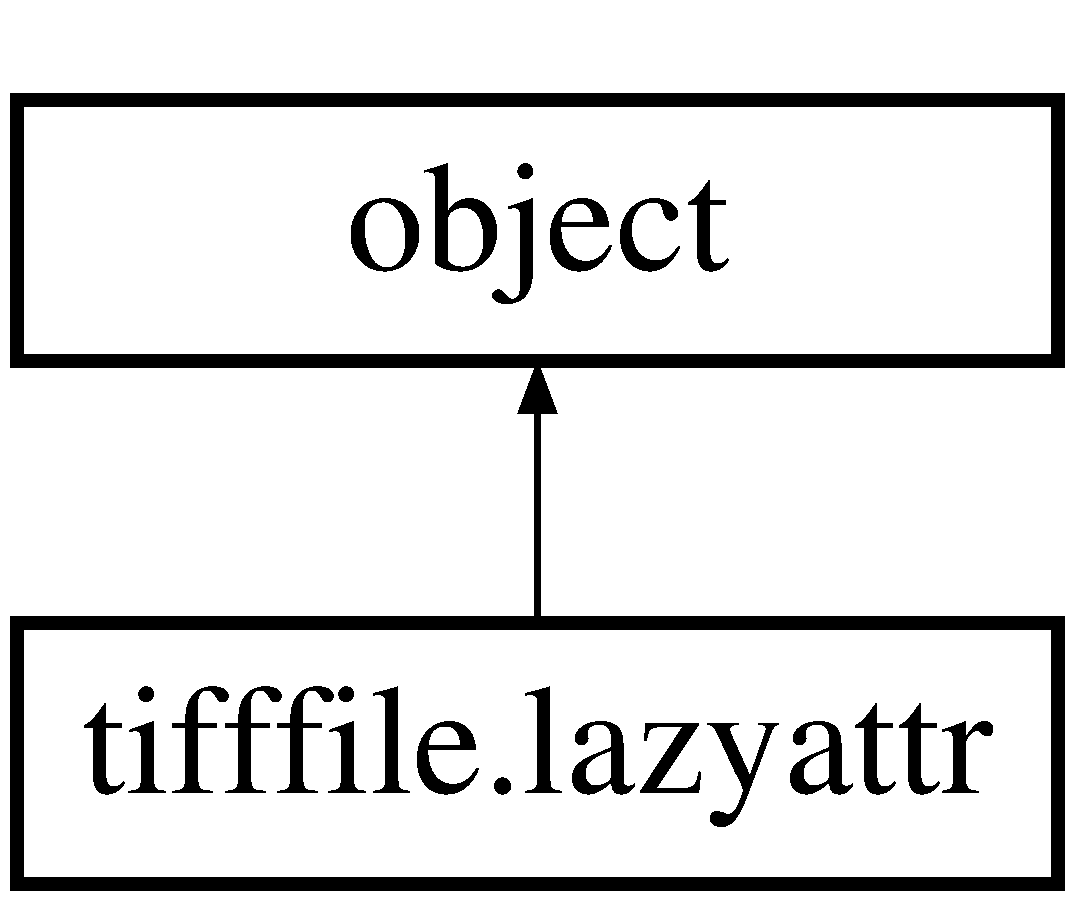
\includegraphics[height=2.000000cm]{classtifffile_1_1lazyattr}
\end{center}
\end{figure}
\subsection*{Public Member Functions}
\begin{DoxyCompactItemize}
\item 
\hypertarget{classtifffile_1_1lazyattr_ae6acbd812e166b92c16d5b76dcac5023}{def {\bfseries \-\_\-\-\_\-init\-\_\-\-\_\-}}\label{classtifffile_1_1lazyattr_ae6acbd812e166b92c16d5b76dcac5023}

\item 
\hypertarget{classtifffile_1_1lazyattr_ab4c827b46c8833a1cb92b6282c8a9365}{def {\bfseries \-\_\-\-\_\-get\-\_\-\-\_\-}}\label{classtifffile_1_1lazyattr_ab4c827b46c8833a1cb92b6282c8a9365}

\end{DoxyCompactItemize}
\subsection*{Public Attributes}
\begin{DoxyCompactItemize}
\item 
\hypertarget{classtifffile_1_1lazyattr_a2d8c47f2babd83fd5d0ca2135a63e6a4}{{\bfseries func}}\label{classtifffile_1_1lazyattr_a2d8c47f2babd83fd5d0ca2135a63e6a4}

\end{DoxyCompactItemize}


\subsection{Detailed Description}
\begin{DoxyVerb}Lazy object attribute whose value is computed on first access.\end{DoxyVerb}
 

The documentation for this class was generated from the following file\-:\begin{DoxyCompactItemize}
\item 
/home/harold/workdir/atrex/\-Software/tifffile.\-py\end{DoxyCompactItemize}

\hypertarget{classmpfit_1_1machar}{\section{mpfit.\-machar Class Reference}
\label{classmpfit_1_1machar}\index{mpfit.\-machar@{mpfit.\-machar}}
}
\subsection*{Public Member Functions}
\begin{DoxyCompactItemize}
\item 
def \hyperlink{classmpfit_1_1machar_a107a955a7c4b29ad883a7c95a564479b}{\-\_\-\-\_\-init\-\_\-\-\_\-}
\end{DoxyCompactItemize}
\subsection*{Public Attributes}
\begin{DoxyCompactItemize}
\item 
\hyperlink{classmpfit_1_1machar_a3f4c542f8c12eadb7fd7899b85e7418f}{machep}
\item 
\hyperlink{classmpfit_1_1machar_ab572a985f979d3940525b5867deafb86}{maxnum}
\item 
\hyperlink{classmpfit_1_1machar_a81a54c7e41c2ef0471983156b9d18b19}{minnum}
\item 
\hyperlink{classmpfit_1_1machar_a038d6337e708014cfb3efedc9fdb4fc8}{maxlog}
\item 
\hyperlink{classmpfit_1_1machar_af01c85a38dbf4a94ae46170e4306baf9}{minlog}
\item 
\hyperlink{classmpfit_1_1machar_ae0d8c6eebbf9deca09bcbc893d5e0428}{rdwarf}
\item 
\hyperlink{classmpfit_1_1machar_ab78cc8c341cd8a39922aa13341be9df9}{rgiant}
\end{DoxyCompactItemize}


\subsection{Constructor \& Destructor Documentation}
\hypertarget{classmpfit_1_1machar_a107a955a7c4b29ad883a7c95a564479b}{\index{mpfit\-::machar@{mpfit\-::machar}!\-\_\-\-\_\-init\-\_\-\-\_\-@{\-\_\-\-\_\-init\-\_\-\-\_\-}}
\index{\-\_\-\-\_\-init\-\_\-\-\_\-@{\-\_\-\-\_\-init\-\_\-\-\_\-}!mpfit::machar@{mpfit\-::machar}}
\subsubsection[{\-\_\-\-\_\-init\-\_\-\-\_\-}]{\setlength{\rightskip}{0pt plus 5cm}def mpfit.\-machar.\-\_\-\-\_\-init\-\_\-\-\_\- (
\begin{DoxyParamCaption}
\item[{}]{self, }
\item[{}]{double = {\ttfamily 1}}
\end{DoxyParamCaption}
)}}\label{classmpfit_1_1machar_a107a955a7c4b29ad883a7c95a564479b}


\subsection{Member Data Documentation}
\hypertarget{classmpfit_1_1machar_a3f4c542f8c12eadb7fd7899b85e7418f}{\index{mpfit\-::machar@{mpfit\-::machar}!machep@{machep}}
\index{machep@{machep}!mpfit::machar@{mpfit\-::machar}}
\subsubsection[{machep}]{\setlength{\rightskip}{0pt plus 5cm}mpfit.\-machar.\-machep}}\label{classmpfit_1_1machar_a3f4c542f8c12eadb7fd7899b85e7418f}
\hypertarget{classmpfit_1_1machar_a038d6337e708014cfb3efedc9fdb4fc8}{\index{mpfit\-::machar@{mpfit\-::machar}!maxlog@{maxlog}}
\index{maxlog@{maxlog}!mpfit::machar@{mpfit\-::machar}}
\subsubsection[{maxlog}]{\setlength{\rightskip}{0pt plus 5cm}mpfit.\-machar.\-maxlog}}\label{classmpfit_1_1machar_a038d6337e708014cfb3efedc9fdb4fc8}
\hypertarget{classmpfit_1_1machar_ab572a985f979d3940525b5867deafb86}{\index{mpfit\-::machar@{mpfit\-::machar}!maxnum@{maxnum}}
\index{maxnum@{maxnum}!mpfit::machar@{mpfit\-::machar}}
\subsubsection[{maxnum}]{\setlength{\rightskip}{0pt plus 5cm}mpfit.\-machar.\-maxnum}}\label{classmpfit_1_1machar_ab572a985f979d3940525b5867deafb86}
\hypertarget{classmpfit_1_1machar_af01c85a38dbf4a94ae46170e4306baf9}{\index{mpfit\-::machar@{mpfit\-::machar}!minlog@{minlog}}
\index{minlog@{minlog}!mpfit::machar@{mpfit\-::machar}}
\subsubsection[{minlog}]{\setlength{\rightskip}{0pt plus 5cm}mpfit.\-machar.\-minlog}}\label{classmpfit_1_1machar_af01c85a38dbf4a94ae46170e4306baf9}
\hypertarget{classmpfit_1_1machar_a81a54c7e41c2ef0471983156b9d18b19}{\index{mpfit\-::machar@{mpfit\-::machar}!minnum@{minnum}}
\index{minnum@{minnum}!mpfit::machar@{mpfit\-::machar}}
\subsubsection[{minnum}]{\setlength{\rightskip}{0pt plus 5cm}mpfit.\-machar.\-minnum}}\label{classmpfit_1_1machar_a81a54c7e41c2ef0471983156b9d18b19}
\hypertarget{classmpfit_1_1machar_ae0d8c6eebbf9deca09bcbc893d5e0428}{\index{mpfit\-::machar@{mpfit\-::machar}!rdwarf@{rdwarf}}
\index{rdwarf@{rdwarf}!mpfit::machar@{mpfit\-::machar}}
\subsubsection[{rdwarf}]{\setlength{\rightskip}{0pt plus 5cm}mpfit.\-machar.\-rdwarf}}\label{classmpfit_1_1machar_ae0d8c6eebbf9deca09bcbc893d5e0428}
\hypertarget{classmpfit_1_1machar_ab78cc8c341cd8a39922aa13341be9df9}{\index{mpfit\-::machar@{mpfit\-::machar}!rgiant@{rgiant}}
\index{rgiant@{rgiant}!mpfit::machar@{mpfit\-::machar}}
\subsubsection[{rgiant}]{\setlength{\rightskip}{0pt plus 5cm}mpfit.\-machar.\-rgiant}}\label{classmpfit_1_1machar_ab78cc8c341cd8a39922aa13341be9df9}


The documentation for this class was generated from the following file\-:\begin{DoxyCompactItemize}
\item 
workdir/atrex/\-Software/\hyperlink{mpfit_8py}{mpfit.\-py}\end{DoxyCompactItemize}

\hypertarget{classMainPeaks_1_1MainPeaks}{\section{Main\-Peaks.\-Main\-Peaks Class Reference}
\label{classMainPeaks_1_1MainPeaks}\index{Main\-Peaks.\-Main\-Peaks@{Main\-Peaks.\-Main\-Peaks}}
}
\subsection*{Public Member Functions}
\begin{DoxyCompactItemize}
\item 
\hypertarget{classMainPeaks_1_1MainPeaks_a8a133d3ee42e272cee3c30d8a1bb6b56}{def {\bfseries \-\_\-\-\_\-init\-\_\-\-\_\-}}\label{classMainPeaks_1_1MainPeaks_a8a133d3ee42e272cee3c30d8a1bb6b56}

\item 
\hypertarget{classMainPeaks_1_1MainPeaks_a6c85bd1ad41c9737aa86d98e447965b2}{def {\bfseries set\-Image}}\label{classMainPeaks_1_1MainPeaks_a6c85bd1ad41c9737aa86d98e447965b2}

\item 
\hypertarget{classMainPeaks_1_1MainPeaks_af353c28f582d469588714fa90f5cefd3}{def {\bfseries peak\-Search}}\label{classMainPeaks_1_1MainPeaks_af353c28f582d469588714fa90f5cefd3}

\item 
\hypertarget{classMainPeaks_1_1MainPeaks_a450255618019c923a86edbe454578f7b}{def {\bfseries write\-Peaks\-To\-File}}\label{classMainPeaks_1_1MainPeaks_a450255618019c923a86edbe454578f7b}

\end{DoxyCompactItemize}
\subsection*{Public Attributes}
\begin{DoxyCompactItemize}
\item 
\hypertarget{classMainPeaks_1_1MainPeaks_a3154ab9972004f57fe2e423781f07452}{{\bfseries myimage}}\label{classMainPeaks_1_1MainPeaks_a3154ab9972004f57fe2e423781f07452}

\item 
\hypertarget{classMainPeaks_1_1MainPeaks_a5c32a36556e49ae19ef9434048cc4a42}{{\bfseries peaks}}\label{classMainPeaks_1_1MainPeaks_a5c32a36556e49ae19ef9434048cc4a42}

\end{DoxyCompactItemize}


The documentation for this class was generated from the following file\-:\begin{DoxyCompactItemize}
\item 
/home/harold/workdir/atrex/\-Software/Main\-Peaks.\-py\end{DoxyCompactItemize}

\hypertarget{classmpfit_1_1mpfit}{\section{mpfit.\-mpfit Class Reference}
\label{classmpfit_1_1mpfit}\index{mpfit.\-mpfit@{mpfit.\-mpfit}}
}
\subsection*{Public Member Functions}
\begin{DoxyCompactItemize}
\item 
def \hyperlink{classmpfit_1_1mpfit_a85f978dd465cf7e718286d24ae6c60a4}{\-\_\-\-\_\-init\-\_\-\-\_\-}
\item 
def \hyperlink{classmpfit_1_1mpfit_a05677996f0b51ba1872c6da189a716b3}{\-\_\-\-\_\-str\-\_\-\-\_\-}
\item 
def \hyperlink{classmpfit_1_1mpfit_a2642766f2780ad122bf6a8da506a3524}{defiter}
\item 
def \hyperlink{classmpfit_1_1mpfit_a4044ca5a6e332785b83426fec482dcf9}{parinfo}
\item 
def \hyperlink{classmpfit_1_1mpfit_a4a57197c1a780d1802d635aaa071ca0c}{call}
\item 
def \hyperlink{classmpfit_1_1mpfit_aacd12e70b3688a26daeece9c2d2f3bf2}{enorm}
\item 
def \hyperlink{classmpfit_1_1mpfit_a4d85cdc05b2d972f319ec1c336337906}{fdjac2}
\item 
def \hyperlink{classmpfit_1_1mpfit_a58e4954f7b62f1e53b2119a3781e03fd}{qrfac}
\item 
def \hyperlink{classmpfit_1_1mpfit_a68e859946e64a6d998b7f48cd0949875}{qrsolv}
\item 
def \hyperlink{classmpfit_1_1mpfit_abb9d174821c887e5d5aa2ca2cc7519f7}{lmpar}
\item 
def \hyperlink{classmpfit_1_1mpfit_a68b9dc3249164597f0d8ed1f6f889ebf}{tie}
\item 
def \hyperlink{classmpfit_1_1mpfit_a217e3eaade969816474f06387c0002ae}{calc\-\_\-covar}
\end{DoxyCompactItemize}
\subsection*{Public Attributes}
\begin{DoxyCompactItemize}
\item 
\hyperlink{classmpfit_1_1mpfit_a0acb816b501c7c62de9b40d51ed3e019}{niter}
\item 
\hyperlink{classmpfit_1_1mpfit_aeeab3c562889cb4fe9d347eeb7e8b40e}{params}
\item 
\hyperlink{classmpfit_1_1mpfit_a6e2df0f73518da9c1bfb3b6c7049bf19}{covar}
\item 
\hyperlink{classmpfit_1_1mpfit_a7fd7c6e0276941f29ae138be862c05fa}{perror}
\item 
\hyperlink{classmpfit_1_1mpfit_a07bef52fd34a9c9d76d605d5d5ff6e6e}{status}
\item 
\hyperlink{classmpfit_1_1mpfit_a358f9f890ac24bb17cf324dd769a69cb}{debug}
\item 
\hyperlink{classmpfit_1_1mpfit_ae0e12388314fd29ceeada36c1f706f53}{errmsg}
\item 
\hyperlink{classmpfit_1_1mpfit_a4a63457ae8102a51227f7ebae4d1d63d}{nfev}
\item 
\hyperlink{classmpfit_1_1mpfit_aef26cc875dbd46374c00332953bb556e}{damp}
\item 
\hyperlink{classmpfit_1_1mpfit_a921637d44c54727c9434aada7f2fc8fb}{dof}
\item 
\hyperlink{classmpfit_1_1mpfit_a69fbce6bf57f692544b35f71d6ae1a07}{fnorm}
\item 
\hyperlink{classmpfit_1_1mpfit_a88c16eda6a0a5ddf3296b1b2d82eba06}{qanytied}
\item 
\hyperlink{classmpfit_1_1mpfit_a121863b0d2d0ffca2d375b7a6f19a567}{ptied}
\item 
\hyperlink{classmpfit_1_1mpfit_a3b940dde9105271118b2e88d9ed88740}{machar}
\item 
\hyperlink{classmpfit_1_1mpfit_ab275d6a4b396b11b4a21d9af891b385f}{blas\-\_\-enorm}
\end{DoxyCompactItemize}


\subsection{Constructor \& Destructor Documentation}
\hypertarget{classmpfit_1_1mpfit_a85f978dd465cf7e718286d24ae6c60a4}{\index{mpfit\-::mpfit@{mpfit\-::mpfit}!\-\_\-\-\_\-init\-\_\-\-\_\-@{\-\_\-\-\_\-init\-\_\-\-\_\-}}
\index{\-\_\-\-\_\-init\-\_\-\-\_\-@{\-\_\-\-\_\-init\-\_\-\-\_\-}!mpfit::mpfit@{mpfit\-::mpfit}}
\subsubsection[{\-\_\-\-\_\-init\-\_\-\-\_\-}]{\setlength{\rightskip}{0pt plus 5cm}def mpfit.\-mpfit.\-\_\-\-\_\-init\-\_\-\-\_\- (
\begin{DoxyParamCaption}
\item[{}]{self, }
\item[{}]{fcn, }
\item[{}]{xall = {\ttfamily None}, }
\item[{}]{functkw = {\ttfamily \{\}}, }
\item[{}]{parinfo = {\ttfamily None}, }
\item[{}]{ftol = {\ttfamily 1.e-\/10}, }
\item[{}]{xtol = {\ttfamily 1.e-\/10}, }
\item[{}]{gtol = {\ttfamily 1.e-\/10}, }
\item[{}]{damp = {\ttfamily 0.}, }
\item[{}]{maxiter = {\ttfamily 200}, }
\item[{}]{factor = {\ttfamily 100.}, }
\item[{}]{nprint = {\ttfamily 1}, }
\item[{}]{iterfunct = {\ttfamily 'default'}, }
\item[{}]{iterkw = {\ttfamily \{\}}, }
\item[{}]{nocovar = {\ttfamily 0}, }
\item[{}]{rescale = {\ttfamily 0}, }
\item[{}]{autoderivative = {\ttfamily 1}, }
\item[{}]{quiet = {\ttfamily 0}, }
\item[{}]{diag = {\ttfamily None}, }
\item[{}]{epsfcn = {\ttfamily None}, }
\item[{}]{debug = {\ttfamily 0}}
\end{DoxyParamCaption}
)}}\label{classmpfit_1_1mpfit_a85f978dd465cf7e718286d24ae6c60a4}
\begin{DoxyVerb}  Inputs:
    fcn:
       The function to be minimized.  The function should return the weighted
       deviations between the model and the data, as described above.

    xall:
       An array of starting values for each of the parameters of the model.
       The number of parameters should be fewer than the number of measurements.

       This parameter is optional if the parinfo keyword is used (but see
       parinfo).  The parinfo keyword provides a mechanism to fix or constrain
       individual parameters.

  Keywords:

     autoderivative:
If this is set, derivatives of the function will be computed
automatically via a finite differencing procedure.  If not set, then
fcn must provide the (analytical) derivatives.
   Default: set (=1)
   NOTE: to supply your own analytical derivatives,
 explicitly pass autoderivative=0

     ftol:
A nonnegative input variable. Termination occurs when both the actual
and predicted relative reductions in the sum of squares are at most
ftol (and status is accordingly set to 1 or 3).  Therefore, ftol
measures the relative error desired in the sum of squares.
   Default: 1E-10

     functkw:
A dictionary which contains the parameters to be passed to the
user-supplied function specified by fcn via the standard Python
keyword dictionary mechanism.  This is the way you can pass additional
data to your user-supplied function without using global variables.

Consider the following example:
   if functkw = {'xval':[1.,2.,3.], 'yval':[1.,4.,9.],
         'errval':[1.,1.,1.] }
then the user supplied function should be declared like this:
   def myfunct(p, fjac=None, xval=None, yval=None, errval=None):

Default: {}   No extra parameters are passed to the user-supplied
      function.

     gtol:
A nonnegative input variable. Termination occurs when the cosine of
the angle between fvec and any column of the jacobian is at most gtol
in absolute value (and status is accordingly set to 4). Therefore,
gtol measures the orthogonality desired between the function vector
and the columns of the jacobian.
   Default: 1e-10

     iterkw:
The keyword arguments to be passed to iterfunct via the dictionary
keyword mechanism.  This should be a dictionary and is similar in
operation to FUNCTKW.
   Default: {}  No arguments are passed.

     iterfunct:
The name of a function to be called upon each NPRINT iteration of the
MPFIT routine.  It should be declared in the following way:
   def iterfunct(myfunct, p, iter, fnorm, functkw=None,
         parinfo=None, quiet=0, dof=None, [iterkw keywords here])
   # perform custom iteration update

iterfunct must accept all three keyword parameters (FUNCTKW, PARINFO
and QUIET).

myfunct:  The user-supplied function to be minimized,
p:      The current set of model parameters
iter:    The iteration number
functkw:  The arguments to be passed to myfunct.
fnorm:  The chi-squared value.
quiet:  Set when no textual output should be printed.
dof:      The number of degrees of freedom, normally the number of points
  less the number of free parameters.
See below for documentation of parinfo.

In implementation, iterfunct can perform updates to the terminal or
graphical user interface, to provide feedback while the fit proceeds.
If the fit is to be stopped for any reason, then iterfunct should return a
a status value between -15 and -1.  Otherwise it should return None
(e.g. no return statement) or 0.
In principle, iterfunct should probably not modify the parameter values,
because it may interfere with the algorithm's stability.  In practice it
is allowed.

Default: an internal routine is used to print the parameter values.

Set iterfunct=None if there is no user-defined routine and you don't
want the internal default routine be called.

     maxiter:
The maximum number of iterations to perform.  If the number is exceeded,
then the status value is set to 5 and MPFIT returns.
Default: 200 iterations

     nocovar:
Set this keyword to prevent the calculation of the covariance matrix
before returning (see COVAR)
Default: clear (=0)  The covariance matrix is returned

     nprint:
The frequency with which iterfunct is called.  A value of 1 indicates
that iterfunct is called with every iteration, while 2 indicates every
other iteration, etc.  Note that several Levenberg-Marquardt attempts
can be made in a single iteration.
Default value: 1

     parinfo
Provides a mechanism for more sophisticated constraints to be placed on
parameter values.  When parinfo is not passed, then it is assumed that
all parameters are free and unconstrained.  Values in parinfo are never
modified during a call to MPFIT.

See description above for the structure of PARINFO.

Default value: None  All parameters are free and unconstrained.

     quiet:
Set this keyword when no textual output should be printed by MPFIT

     damp:
A scalar number, indicating the cut-off value of residuals where
"damping" will occur.  Residuals with magnitudes greater than this
number will be replaced by their hyperbolic tangent.  This partially
mitigates the so-called large residual problem inherent in
least-squares solvers (as for the test problem CURVI,
http://www.maxthis.com/curviex.htm).
A value of 0 indicates no damping.
   Default: 0

Note: DAMP doesn't work with autoderivative=0

     xtol:
A nonnegative input variable. Termination occurs when the relative error
between two consecutive iterates is at most xtol (and status is
accordingly set to 2 or 3).  Therefore, xtol measures the relative error
desired in the approximate solution.
Default: 1E-10

   Outputs:

     Returns an object of type mpfit.  The results are attributes of this class,
     e.g. mpfit.status, mpfit.errmsg, mpfit.params, npfit.niter, mpfit.covar.

     .status
An integer status code is returned.  All values greater than zero can
represent success (however .status == 5 may indicate failure to
converge). It can have one of the following values:

-16
   A parameter or function value has become infinite or an undefined
   number.  This is usually a consequence of numerical overflow in the
   user's model function, which must be avoided.

-15 to -1
   These are error codes that either MYFUNCT or iterfunct may return to
   terminate the fitting process.  Values from -15 to -1 are reserved
   for the user functions and will not clash with MPFIT.

0  Improper input parameters.

1  Both actual and predicted relative reductions in the sum of squares
   are at most ftol.

2  Relative error between two consecutive iterates is at most xtol

3  Conditions for status = 1 and status = 2 both hold.

4  The cosine of the angle between fvec and any column of the jacobian
   is at most gtol in absolute value.

5  The maximum number of iterations has been reached.

6  ftol is too small. No further reduction in the sum of squares is
   possible.

7  xtol is too small. No further improvement in the approximate solution
   x is possible.

8  gtol is too small. fvec is orthogonal to the columns of the jacobian
   to machine precision.

     .fnorm
The value of the summed squared residuals for the returned parameter
values.

     .covar
The covariance matrix for the set of parameters returned by MPFIT.
The matrix is NxN where N is the number of  parameters.  The square root
of the diagonal elements gives the formal 1-sigma statistical errors on
the parameters if errors were treated "properly" in fcn.
Parameter errors are also returned in .perror.

To compute the correlation matrix, pcor, use this example:
   cov = mpfit.covar
   pcor = cov * 0.
   for i in range(n):
      for j in range(n):
 pcor[i,j] = cov[i,j]/sqrt(cov[i,i]*cov[j,j])

If nocovar is set or MPFIT terminated abnormally, then .covar is set to
a scalar with value None.

     .errmsg
A string error or warning message is returned.

     .nfev
The number of calls to MYFUNCT performed.

     .niter
The number of iterations completed.

     .perror
The formal 1-sigma errors in each parameter, computed from the
covariance matrix.  If a parameter is held fixed, or if it touches a
boundary, then the error is reported as zero.

If the fit is unweighted (i.e. no errors were given, or the weights
were uniformly set to unity), then .perror will probably not represent
the true parameter uncertainties.

*If* you can assume that the true reduced chi-squared value is unity --
meaning that the fit is implicitly assumed to be of good quality --
then the estimated parameter uncertainties can be computed by scaling
.perror by the measured chi-squared value.

   dof = len(x) - len(mpfit.params) # deg of freedom
   # scaled uncertainties
   pcerror = mpfit.perror * sqrt(mpfit.fnorm / dof)\end{DoxyVerb}
 

\subsection{Member Function Documentation}
\hypertarget{classmpfit_1_1mpfit_a05677996f0b51ba1872c6da189a716b3}{\index{mpfit\-::mpfit@{mpfit\-::mpfit}!\-\_\-\-\_\-str\-\_\-\-\_\-@{\-\_\-\-\_\-str\-\_\-\-\_\-}}
\index{\-\_\-\-\_\-str\-\_\-\-\_\-@{\-\_\-\-\_\-str\-\_\-\-\_\-}!mpfit::mpfit@{mpfit\-::mpfit}}
\subsubsection[{\-\_\-\-\_\-str\-\_\-\-\_\-}]{\setlength{\rightskip}{0pt plus 5cm}def mpfit.\-mpfit.\-\_\-\-\_\-str\-\_\-\-\_\- (
\begin{DoxyParamCaption}
\item[{}]{self}
\end{DoxyParamCaption}
)}}\label{classmpfit_1_1mpfit_a05677996f0b51ba1872c6da189a716b3}
\hypertarget{classmpfit_1_1mpfit_a217e3eaade969816474f06387c0002ae}{\index{mpfit\-::mpfit@{mpfit\-::mpfit}!calc\-\_\-covar@{calc\-\_\-covar}}
\index{calc\-\_\-covar@{calc\-\_\-covar}!mpfit::mpfit@{mpfit\-::mpfit}}
\subsubsection[{calc\-\_\-covar}]{\setlength{\rightskip}{0pt plus 5cm}def mpfit.\-mpfit.\-calc\-\_\-covar (
\begin{DoxyParamCaption}
\item[{}]{self, }
\item[{}]{rr, }
\item[{}]{ipvt = {\ttfamily None}, }
\item[{}]{tol = {\ttfamily 1.e-\/14}}
\end{DoxyParamCaption}
)}}\label{classmpfit_1_1mpfit_a217e3eaade969816474f06387c0002ae}
\hypertarget{classmpfit_1_1mpfit_a4a57197c1a780d1802d635aaa071ca0c}{\index{mpfit\-::mpfit@{mpfit\-::mpfit}!call@{call}}
\index{call@{call}!mpfit::mpfit@{mpfit\-::mpfit}}
\subsubsection[{call}]{\setlength{\rightskip}{0pt plus 5cm}def mpfit.\-mpfit.\-call (
\begin{DoxyParamCaption}
\item[{}]{self, }
\item[{}]{fcn, }
\item[{}]{x, }
\item[{}]{functkw, }
\item[{}]{fjac = {\ttfamily None}}
\end{DoxyParamCaption}
)}}\label{classmpfit_1_1mpfit_a4a57197c1a780d1802d635aaa071ca0c}
\hypertarget{classmpfit_1_1mpfit_a2642766f2780ad122bf6a8da506a3524}{\index{mpfit\-::mpfit@{mpfit\-::mpfit}!defiter@{defiter}}
\index{defiter@{defiter}!mpfit::mpfit@{mpfit\-::mpfit}}
\subsubsection[{defiter}]{\setlength{\rightskip}{0pt plus 5cm}def mpfit.\-mpfit.\-defiter (
\begin{DoxyParamCaption}
\item[{}]{self, }
\item[{}]{fcn, }
\item[{}]{x, }
\item[{}]{iter, }
\item[{}]{fnorm = {\ttfamily None}, }
\item[{}]{functkw = {\ttfamily None}, }
\item[{}]{quiet = {\ttfamily 0}, }
\item[{}]{iterstop = {\ttfamily None}, }
\item[{}]{parinfo = {\ttfamily None}, }
\item[{}]{format = {\ttfamily None}, }
\item[{}]{pformat = {\ttfamily '\%.10g'}, }
\item[{}]{dof = {\ttfamily 1}}
\end{DoxyParamCaption}
)}}\label{classmpfit_1_1mpfit_a2642766f2780ad122bf6a8da506a3524}
\hypertarget{classmpfit_1_1mpfit_aacd12e70b3688a26daeece9c2d2f3bf2}{\index{mpfit\-::mpfit@{mpfit\-::mpfit}!enorm@{enorm}}
\index{enorm@{enorm}!mpfit::mpfit@{mpfit\-::mpfit}}
\subsubsection[{enorm}]{\setlength{\rightskip}{0pt plus 5cm}def mpfit.\-mpfit.\-enorm (
\begin{DoxyParamCaption}
\item[{}]{self, }
\item[{}]{vec}
\end{DoxyParamCaption}
)}}\label{classmpfit_1_1mpfit_aacd12e70b3688a26daeece9c2d2f3bf2}
\hypertarget{classmpfit_1_1mpfit_a4d85cdc05b2d972f319ec1c336337906}{\index{mpfit\-::mpfit@{mpfit\-::mpfit}!fdjac2@{fdjac2}}
\index{fdjac2@{fdjac2}!mpfit::mpfit@{mpfit\-::mpfit}}
\subsubsection[{fdjac2}]{\setlength{\rightskip}{0pt plus 5cm}def mpfit.\-mpfit.\-fdjac2 (
\begin{DoxyParamCaption}
\item[{}]{self, }
\item[{}]{fcn, }
\item[{}]{x, }
\item[{}]{fvec, }
\item[{}]{step = {\ttfamily None}, }
\item[{}]{ulimited = {\ttfamily None}, }
\item[{}]{ulimit = {\ttfamily None}, }
\item[{}]{dside = {\ttfamily None}, }
\item[{}]{epsfcn = {\ttfamily None}, }
\item[{}]{autoderivative = {\ttfamily 1}, }
\item[{}]{functkw = {\ttfamily None}, }
\item[{}]{xall = {\ttfamily None}, }
\item[{}]{ifree = {\ttfamily None}, }
\item[{}]{dstep = {\ttfamily None}}
\end{DoxyParamCaption}
)}}\label{classmpfit_1_1mpfit_a4d85cdc05b2d972f319ec1c336337906}
\hypertarget{classmpfit_1_1mpfit_abb9d174821c887e5d5aa2ca2cc7519f7}{\index{mpfit\-::mpfit@{mpfit\-::mpfit}!lmpar@{lmpar}}
\index{lmpar@{lmpar}!mpfit::mpfit@{mpfit\-::mpfit}}
\subsubsection[{lmpar}]{\setlength{\rightskip}{0pt plus 5cm}def mpfit.\-mpfit.\-lmpar (
\begin{DoxyParamCaption}
\item[{}]{self, }
\item[{}]{r, }
\item[{}]{ipvt, }
\item[{}]{diag, }
\item[{}]{qtb, }
\item[{}]{delta, }
\item[{}]{x, }
\item[{}]{sdiag, }
\item[{}]{par = {\ttfamily None}}
\end{DoxyParamCaption}
)}}\label{classmpfit_1_1mpfit_abb9d174821c887e5d5aa2ca2cc7519f7}
\hypertarget{classmpfit_1_1mpfit_a4044ca5a6e332785b83426fec482dcf9}{\index{mpfit\-::mpfit@{mpfit\-::mpfit}!parinfo@{parinfo}}
\index{parinfo@{parinfo}!mpfit::mpfit@{mpfit\-::mpfit}}
\subsubsection[{parinfo}]{\setlength{\rightskip}{0pt plus 5cm}def mpfit.\-mpfit.\-parinfo (
\begin{DoxyParamCaption}
\item[{}]{self, }
\item[{}]{parinfo = {\ttfamily None}, }
\item[{}]{key = {\ttfamily 'a'}, }
\item[{}]{default = {\ttfamily None}, }
\item[{}]{n = {\ttfamily 0}}
\end{DoxyParamCaption}
)}}\label{classmpfit_1_1mpfit_a4044ca5a6e332785b83426fec482dcf9}
\hypertarget{classmpfit_1_1mpfit_a58e4954f7b62f1e53b2119a3781e03fd}{\index{mpfit\-::mpfit@{mpfit\-::mpfit}!qrfac@{qrfac}}
\index{qrfac@{qrfac}!mpfit::mpfit@{mpfit\-::mpfit}}
\subsubsection[{qrfac}]{\setlength{\rightskip}{0pt plus 5cm}def mpfit.\-mpfit.\-qrfac (
\begin{DoxyParamCaption}
\item[{}]{self, }
\item[{}]{a, }
\item[{}]{pivot = {\ttfamily 0}}
\end{DoxyParamCaption}
)}}\label{classmpfit_1_1mpfit_a58e4954f7b62f1e53b2119a3781e03fd}
\hypertarget{classmpfit_1_1mpfit_a68e859946e64a6d998b7f48cd0949875}{\index{mpfit\-::mpfit@{mpfit\-::mpfit}!qrsolv@{qrsolv}}
\index{qrsolv@{qrsolv}!mpfit::mpfit@{mpfit\-::mpfit}}
\subsubsection[{qrsolv}]{\setlength{\rightskip}{0pt plus 5cm}def mpfit.\-mpfit.\-qrsolv (
\begin{DoxyParamCaption}
\item[{}]{self, }
\item[{}]{r, }
\item[{}]{ipvt, }
\item[{}]{diag, }
\item[{}]{qtb, }
\item[{}]{sdiag}
\end{DoxyParamCaption}
)}}\label{classmpfit_1_1mpfit_a68e859946e64a6d998b7f48cd0949875}
\hypertarget{classmpfit_1_1mpfit_a68b9dc3249164597f0d8ed1f6f889ebf}{\index{mpfit\-::mpfit@{mpfit\-::mpfit}!tie@{tie}}
\index{tie@{tie}!mpfit::mpfit@{mpfit\-::mpfit}}
\subsubsection[{tie}]{\setlength{\rightskip}{0pt plus 5cm}def mpfit.\-mpfit.\-tie (
\begin{DoxyParamCaption}
\item[{}]{self, }
\item[{}]{p, }
\item[{}]{ptied = {\ttfamily None}}
\end{DoxyParamCaption}
)}}\label{classmpfit_1_1mpfit_a68b9dc3249164597f0d8ed1f6f889ebf}


\subsection{Member Data Documentation}
\hypertarget{classmpfit_1_1mpfit_ab275d6a4b396b11b4a21d9af891b385f}{\index{mpfit\-::mpfit@{mpfit\-::mpfit}!blas\-\_\-enorm@{blas\-\_\-enorm}}
\index{blas\-\_\-enorm@{blas\-\_\-enorm}!mpfit::mpfit@{mpfit\-::mpfit}}
\subsubsection[{blas\-\_\-enorm}]{\setlength{\rightskip}{0pt plus 5cm}mpfit.\-mpfit.\-blas\-\_\-enorm}}\label{classmpfit_1_1mpfit_ab275d6a4b396b11b4a21d9af891b385f}
\hypertarget{classmpfit_1_1mpfit_a6e2df0f73518da9c1bfb3b6c7049bf19}{\index{mpfit\-::mpfit@{mpfit\-::mpfit}!covar@{covar}}
\index{covar@{covar}!mpfit::mpfit@{mpfit\-::mpfit}}
\subsubsection[{covar}]{\setlength{\rightskip}{0pt plus 5cm}mpfit.\-mpfit.\-covar}}\label{classmpfit_1_1mpfit_a6e2df0f73518da9c1bfb3b6c7049bf19}
\hypertarget{classmpfit_1_1mpfit_aef26cc875dbd46374c00332953bb556e}{\index{mpfit\-::mpfit@{mpfit\-::mpfit}!damp@{damp}}
\index{damp@{damp}!mpfit::mpfit@{mpfit\-::mpfit}}
\subsubsection[{damp}]{\setlength{\rightskip}{0pt plus 5cm}mpfit.\-mpfit.\-damp}}\label{classmpfit_1_1mpfit_aef26cc875dbd46374c00332953bb556e}
\hypertarget{classmpfit_1_1mpfit_a358f9f890ac24bb17cf324dd769a69cb}{\index{mpfit\-::mpfit@{mpfit\-::mpfit}!debug@{debug}}
\index{debug@{debug}!mpfit::mpfit@{mpfit\-::mpfit}}
\subsubsection[{debug}]{\setlength{\rightskip}{0pt plus 5cm}mpfit.\-mpfit.\-debug}}\label{classmpfit_1_1mpfit_a358f9f890ac24bb17cf324dd769a69cb}
\hypertarget{classmpfit_1_1mpfit_a921637d44c54727c9434aada7f2fc8fb}{\index{mpfit\-::mpfit@{mpfit\-::mpfit}!dof@{dof}}
\index{dof@{dof}!mpfit::mpfit@{mpfit\-::mpfit}}
\subsubsection[{dof}]{\setlength{\rightskip}{0pt plus 5cm}mpfit.\-mpfit.\-dof}}\label{classmpfit_1_1mpfit_a921637d44c54727c9434aada7f2fc8fb}
\hypertarget{classmpfit_1_1mpfit_ae0e12388314fd29ceeada36c1f706f53}{\index{mpfit\-::mpfit@{mpfit\-::mpfit}!errmsg@{errmsg}}
\index{errmsg@{errmsg}!mpfit::mpfit@{mpfit\-::mpfit}}
\subsubsection[{errmsg}]{\setlength{\rightskip}{0pt plus 5cm}mpfit.\-mpfit.\-errmsg}}\label{classmpfit_1_1mpfit_ae0e12388314fd29ceeada36c1f706f53}
\hypertarget{classmpfit_1_1mpfit_a69fbce6bf57f692544b35f71d6ae1a07}{\index{mpfit\-::mpfit@{mpfit\-::mpfit}!fnorm@{fnorm}}
\index{fnorm@{fnorm}!mpfit::mpfit@{mpfit\-::mpfit}}
\subsubsection[{fnorm}]{\setlength{\rightskip}{0pt plus 5cm}mpfit.\-mpfit.\-fnorm}}\label{classmpfit_1_1mpfit_a69fbce6bf57f692544b35f71d6ae1a07}
\hypertarget{classmpfit_1_1mpfit_a3b940dde9105271118b2e88d9ed88740}{\index{mpfit\-::mpfit@{mpfit\-::mpfit}!machar@{machar}}
\index{machar@{machar}!mpfit::mpfit@{mpfit\-::mpfit}}
\subsubsection[{machar}]{\setlength{\rightskip}{0pt plus 5cm}mpfit.\-mpfit.\-machar}}\label{classmpfit_1_1mpfit_a3b940dde9105271118b2e88d9ed88740}
\hypertarget{classmpfit_1_1mpfit_a4a63457ae8102a51227f7ebae4d1d63d}{\index{mpfit\-::mpfit@{mpfit\-::mpfit}!nfev@{nfev}}
\index{nfev@{nfev}!mpfit::mpfit@{mpfit\-::mpfit}}
\subsubsection[{nfev}]{\setlength{\rightskip}{0pt plus 5cm}mpfit.\-mpfit.\-nfev}}\label{classmpfit_1_1mpfit_a4a63457ae8102a51227f7ebae4d1d63d}
\hypertarget{classmpfit_1_1mpfit_a0acb816b501c7c62de9b40d51ed3e019}{\index{mpfit\-::mpfit@{mpfit\-::mpfit}!niter@{niter}}
\index{niter@{niter}!mpfit::mpfit@{mpfit\-::mpfit}}
\subsubsection[{niter}]{\setlength{\rightskip}{0pt plus 5cm}mpfit.\-mpfit.\-niter}}\label{classmpfit_1_1mpfit_a0acb816b501c7c62de9b40d51ed3e019}
\hypertarget{classmpfit_1_1mpfit_aeeab3c562889cb4fe9d347eeb7e8b40e}{\index{mpfit\-::mpfit@{mpfit\-::mpfit}!params@{params}}
\index{params@{params}!mpfit::mpfit@{mpfit\-::mpfit}}
\subsubsection[{params}]{\setlength{\rightskip}{0pt plus 5cm}mpfit.\-mpfit.\-params}}\label{classmpfit_1_1mpfit_aeeab3c562889cb4fe9d347eeb7e8b40e}
\hypertarget{classmpfit_1_1mpfit_a7fd7c6e0276941f29ae138be862c05fa}{\index{mpfit\-::mpfit@{mpfit\-::mpfit}!perror@{perror}}
\index{perror@{perror}!mpfit::mpfit@{mpfit\-::mpfit}}
\subsubsection[{perror}]{\setlength{\rightskip}{0pt plus 5cm}mpfit.\-mpfit.\-perror}}\label{classmpfit_1_1mpfit_a7fd7c6e0276941f29ae138be862c05fa}
\hypertarget{classmpfit_1_1mpfit_a121863b0d2d0ffca2d375b7a6f19a567}{\index{mpfit\-::mpfit@{mpfit\-::mpfit}!ptied@{ptied}}
\index{ptied@{ptied}!mpfit::mpfit@{mpfit\-::mpfit}}
\subsubsection[{ptied}]{\setlength{\rightskip}{0pt plus 5cm}mpfit.\-mpfit.\-ptied}}\label{classmpfit_1_1mpfit_a121863b0d2d0ffca2d375b7a6f19a567}
\hypertarget{classmpfit_1_1mpfit_a88c16eda6a0a5ddf3296b1b2d82eba06}{\index{mpfit\-::mpfit@{mpfit\-::mpfit}!qanytied@{qanytied}}
\index{qanytied@{qanytied}!mpfit::mpfit@{mpfit\-::mpfit}}
\subsubsection[{qanytied}]{\setlength{\rightskip}{0pt plus 5cm}mpfit.\-mpfit.\-qanytied}}\label{classmpfit_1_1mpfit_a88c16eda6a0a5ddf3296b1b2d82eba06}
\hypertarget{classmpfit_1_1mpfit_a07bef52fd34a9c9d76d605d5d5ff6e6e}{\index{mpfit\-::mpfit@{mpfit\-::mpfit}!status@{status}}
\index{status@{status}!mpfit::mpfit@{mpfit\-::mpfit}}
\subsubsection[{status}]{\setlength{\rightskip}{0pt plus 5cm}mpfit.\-mpfit.\-status}}\label{classmpfit_1_1mpfit_a07bef52fd34a9c9d76d605d5d5ff6e6e}


The documentation for this class was generated from the following file\-:\begin{DoxyCompactItemize}
\item 
workdir/atrex/\-Software/\hyperlink{mpfit_8py}{mpfit.\-py}\end{DoxyCompactItemize}

\hypertarget{classmyDetector_1_1myDetector}{\section{my\-Detector.\-my\-Detector Class Reference}
\label{classmyDetector_1_1myDetector}\index{my\-Detector.\-my\-Detector@{my\-Detector.\-my\-Detector}}
}
Inheritance diagram for my\-Detector.\-my\-Detector\-:\begin{figure}[H]
\begin{center}
\leavevmode
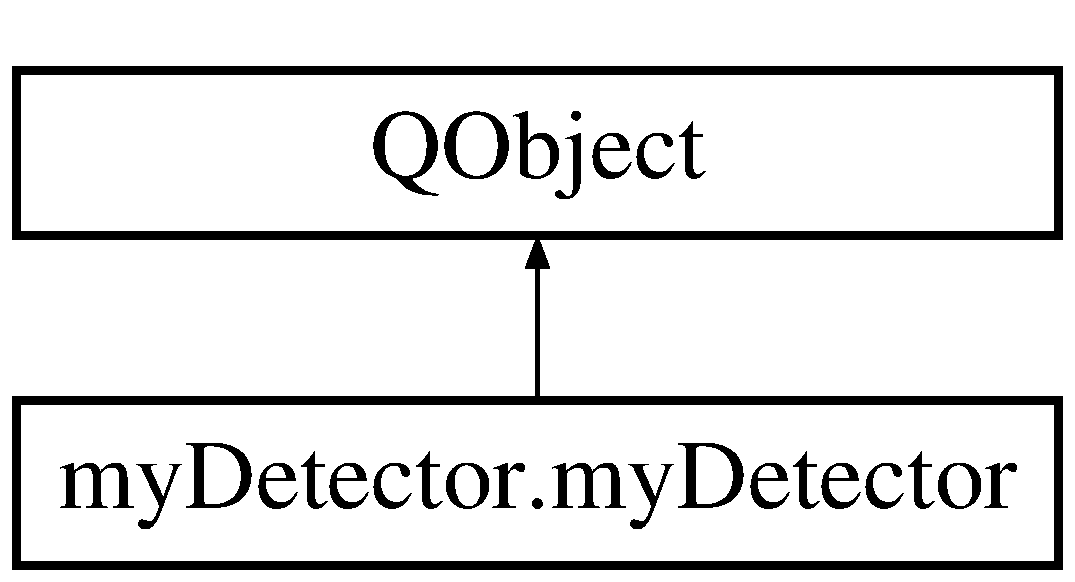
\includegraphics[height=2.000000cm]{classmyDetector_1_1myDetector}
\end{center}
\end{figure}
\subsection*{Public Member Functions}
\begin{DoxyCompactItemize}
\item 
\hypertarget{classmyDetector_1_1myDetector_a783da80204b3f19403a26284d376fc18}{def {\bfseries \-\_\-\-\_\-init\-\_\-\-\_\-}}\label{classmyDetector_1_1myDetector_a783da80204b3f19403a26284d376fc18}

\item 
\hypertarget{classmyDetector_1_1myDetector_ad1237b8f9843336bd470eea90068c001}{def {\bfseries set\-Top\-Level}}\label{classmyDetector_1_1myDetector_ad1237b8f9843336bd470eea90068c001}

\item 
\hypertarget{classmyDetector_1_1myDetector_aa9ba5cd92fa49b0935c8cc5a88adf919}{def {\bfseries getdist}}\label{classmyDetector_1_1myDetector_aa9ba5cd92fa49b0935c8cc5a88adf919}

\item 
\hypertarget{classmyDetector_1_1myDetector_a9dbec7a26b92a1d52144dd9fd99e89a7}{def {\bfseries setdist}}\label{classmyDetector_1_1myDetector_a9dbec7a26b92a1d52144dd9fd99e89a7}

\item 
\hypertarget{classmyDetector_1_1myDetector_a73d637fe6d8f0b6685c9ea07e0444b14}{def {\bfseries getwavelength}}\label{classmyDetector_1_1myDetector_a73d637fe6d8f0b6685c9ea07e0444b14}

\item 
\hypertarget{classmyDetector_1_1myDetector_aa86114f3da1a2f6bf4d8595564654b0c}{def {\bfseries setwavelength}}\label{classmyDetector_1_1myDetector_aa86114f3da1a2f6bf4d8595564654b0c}

\item 
\hypertarget{classmyDetector_1_1myDetector_aa70f5dd1888bee1c70eaa1a1410c4cd9}{def {\bfseries gettiltom}}\label{classmyDetector_1_1myDetector_aa70f5dd1888bee1c70eaa1a1410c4cd9}

\item 
\hypertarget{classmyDetector_1_1myDetector_a2ab94c7245903209b1ec67fe726727f8}{def {\bfseries settiltom}}\label{classmyDetector_1_1myDetector_a2ab94c7245903209b1ec67fe726727f8}

\item 
\hypertarget{classmyDetector_1_1myDetector_a5814f9b4c3659e0c3ca527d2c62d0cb5}{def {\bfseries gettiltch}}\label{classmyDetector_1_1myDetector_a5814f9b4c3659e0c3ca527d2c62d0cb5}

\item 
\hypertarget{classmyDetector_1_1myDetector_a962ed549d7586e474ad70f18b16ee828}{def {\bfseries settiltch}}\label{classmyDetector_1_1myDetector_a962ed549d7586e474ad70f18b16ee828}

\item 
\hypertarget{classmyDetector_1_1myDetector_ae355ac64795c27bec293a55ea1f0f1c5}{def {\bfseries getttheta}}\label{classmyDetector_1_1myDetector_ae355ac64795c27bec293a55ea1f0f1c5}

\item 
\hypertarget{classmyDetector_1_1myDetector_a820154c642e5b92a5b7a71d02f0611cd}{def {\bfseries setttheta}}\label{classmyDetector_1_1myDetector_a820154c642e5b92a5b7a71d02f0611cd}

\item 
\hypertarget{classmyDetector_1_1myDetector_af9f5fe17290771ee89f44d61460788c2}{def {\bfseries gettwist}}\label{classmyDetector_1_1myDetector_af9f5fe17290771ee89f44d61460788c2}

\item 
\hypertarget{classmyDetector_1_1myDetector_aa347097de35029fb149193660848637f}{def {\bfseries settwist}}\label{classmyDetector_1_1myDetector_aa347097de35029fb149193660848637f}

\item 
\hypertarget{classmyDetector_1_1myDetector_a77ca154ee209ba6feea760224b0ccc7f}{def {\bfseries getbeam\-X\-Y}}\label{classmyDetector_1_1myDetector_a77ca154ee209ba6feea760224b0ccc7f}

\item 
\hypertarget{classmyDetector_1_1myDetector_a39df1d613aada63ef323aa4a5ca4fa34}{def {\bfseries setbeam\-X\-Y}}\label{classmyDetector_1_1myDetector_a39df1d613aada63ef323aa4a5ca4fa34}

\item 
\hypertarget{classmyDetector_1_1myDetector_a9c607c43c8f55baa0c6bd7bf356b17a1}{def {\bfseries getpsize\-X\-Y}}\label{classmyDetector_1_1myDetector_a9c607c43c8f55baa0c6bd7bf356b17a1}

\item 
\hypertarget{classmyDetector_1_1myDetector_a9018d849252b07724e9046a615c27e0b}{def {\bfseries setpsize\-X\-Y}}\label{classmyDetector_1_1myDetector_a9018d849252b07724e9046a615c27e0b}

\item 
\hypertarget{classmyDetector_1_1myDetector_a8f5b1f53fa3905551d797312390be7e9}{def {\bfseries getnopix\-X\-Y}}\label{classmyDetector_1_1myDetector_a8f5b1f53fa3905551d797312390be7e9}

\item 
\hypertarget{classmyDetector_1_1myDetector_a17e10421e1beb0ace96f0e0075d923d8}{def {\bfseries setnopix\-X\-Y}}\label{classmyDetector_1_1myDetector_a17e10421e1beb0ace96f0e0075d923d8}

\item 
\hypertarget{classmyDetector_1_1myDetector_a47f4a741e9c43ea2ca937b38d26d85bd}{def {\bfseries write\-\_\-to\-\_\-file}}\label{classmyDetector_1_1myDetector_a47f4a741e9c43ea2ca937b38d26d85bd}

\item 
\hypertarget{classmyDetector_1_1myDetector_a28805fea27eebf5e4b50defd31842d9b}{def {\bfseries read\-\_\-from\-\_\-file}}\label{classmyDetector_1_1myDetector_a28805fea27eebf5e4b50defd31842d9b}

\item 
\hypertarget{classmyDetector_1_1myDetector_a22f02df85f7dd4f30ab64d7e0b204b6a}{def {\bfseries read\-\_\-from\-\_\-text\-\_\-file}}\label{classmyDetector_1_1myDetector_a22f02df85f7dd4f30ab64d7e0b204b6a}

\item 
\hypertarget{classmyDetector_1_1myDetector_a07bb062a70ceaec37614c8877e6ae659}{def {\bfseries write\-\_\-to\-\_\-text\-\_\-file}}\label{classmyDetector_1_1myDetector_a07bb062a70ceaec37614c8877e6ae659}

\item 
\hypertarget{classmyDetector_1_1myDetector_a2f7eb213400bfad0ffd110b060ce2469}{def {\bfseries calculate\-\_\-tth\-\_\-from\-\_\-pixels}}\label{classmyDetector_1_1myDetector_a2f7eb213400bfad0ffd110b060ce2469}

\item 
\hypertarget{classmyDetector_1_1myDetector_ad897737f4883453052f916edaee91ac0}{def {\bfseries calculate\-\_\-pixels\-\_\-from\-\_\-sd}}\label{classmyDetector_1_1myDetector_ad897737f4883453052f916edaee91ac0}

\item 
\hypertarget{classmyDetector_1_1myDetector_a8e63ddf3ddf9aa2972ee936c27788915}{def {\bfseries calculate\-\_\-sd\-\_\-from\-\_\-pixels}}\label{classmyDetector_1_1myDetector_a8e63ddf3ddf9aa2972ee936c27788915}

\item 
\hypertarget{classmyDetector_1_1myDetector_abd5c5ca2d3f99a6759a1a9b670ef6b2e}{def {\bfseries calculate\-\_\-sd\-\_\-from\-\_\-pixels\-\_\-arr}}\label{classmyDetector_1_1myDetector_abd5c5ca2d3f99a6759a1a9b670ef6b2e}

\item 
\hypertarget{classmyDetector_1_1myDetector_a1b53a39b4e53442c2a7f7fb9ee77e156}{def {\bfseries tilt\-\_\-mtx}}\label{classmyDetector_1_1myDetector_a1b53a39b4e53442c2a7f7fb9ee77e156}

\item 
\hypertarget{classmyDetector_1_1myDetector_a91ee215369c918ef83d0c8598daeab46}{def {\bfseries gen\-Tilt\-Mtx}}\label{classmyDetector_1_1myDetector_a91ee215369c918ef83d0c8598daeab46}

\item 
\hypertarget{classmyDetector_1_1myDetector_a089663282c90924b0fc4e2f53bb96aa2}{def {\bfseries calc2theta}}\label{classmyDetector_1_1myDetector_a089663282c90924b0fc4e2f53bb96aa2}

\item 
\hypertarget{classmyDetector_1_1myDetector_a10dd4f576fd9e8cd3cbfb45625a74113}{def {\bfseries test\-Stuff}}\label{classmyDetector_1_1myDetector_a10dd4f576fd9e8cd3cbfb45625a74113}

\item 
\hypertarget{classmyDetector_1_1myDetector_a16783ce90d948c85c5cf0a2930c60a4f}{def {\bfseries create\-\_\-ttheta\-\_\-array}}\label{classmyDetector_1_1myDetector_a16783ce90d948c85c5cf0a2930c60a4f}

\item 
\hypertarget{classmyDetector_1_1myDetector_a9558eaedd3456b1705b8962d861f7b1c}{def {\bfseries create\-\_\-ttheta\-\_\-array\-\_\-sub}}\label{classmyDetector_1_1myDetector_a9558eaedd3456b1705b8962d861f7b1c}

\item 
\hypertarget{classmyDetector_1_1myDetector_ab1ec39dedf5ad3f5e49ecacd935632ee}{def {\bfseries calc\-Tth\-D\-L\-L}}\label{classmyDetector_1_1myDetector_ab1ec39dedf5ad3f5e49ecacd935632ee}

\item 
\hypertarget{classmyDetector_1_1myDetector_afc52520eef732679f7ab195a0722a9e7}{def {\bfseries generate\-\_\-peaks\-\_\-laue}}\label{classmyDetector_1_1myDetector_afc52520eef732679f7ab195a0722a9e7}

\item 
\hypertarget{classmyDetector_1_1myDetector_ab1ec39dedf5ad3f5e49ecacd935632ee}{def {\bfseries calc\-Tth\-D\-L\-L}}\label{classmyDetector_1_1myDetector_ab1ec39dedf5ad3f5e49ecacd935632ee}

\item 
\hypertarget{classmyDetector_1_1myDetector_ae6bc52229c1afb9e5f4d386f65436609}{def {\bfseries thread\-Done\-Slot}}\label{classmyDetector_1_1myDetector_ae6bc52229c1afb9e5f4d386f65436609}

\item 
\hypertarget{classmyDetector_1_1myDetector_a32e75eff3dbfa9bd7aa2c52c35dc5ed9}{def {\bfseries calculate\-\_\-pixels\-\_\-from\-\_\-xyz}}\label{classmyDetector_1_1myDetector_a32e75eff3dbfa9bd7aa2c52c35dc5ed9}

\item 
\hypertarget{classmyDetector_1_1myDetector_a6c37e75cc10b463055607b353c08906a}{def {\bfseries generate\-Rot\-Matrix}}\label{classmyDetector_1_1myDetector_a6c37e75cc10b463055607b353c08906a}

\item 
\hypertarget{classmyDetector_1_1myDetector_ae044536621ae1d67732986d2786e89eb}{def {\bfseries calculate\-\_\-psi\-\_\-angles}}\label{classmyDetector_1_1myDetector_ae044536621ae1d67732986d2786e89eb}

\item 
\hypertarget{classmyDetector_1_1myDetector_a4a11ce6f14f52e3cf63340d91dc819db}{def {\bfseries generate\-\_\-all\-\_\-peaks}}\label{classmyDetector_1_1myDetector_a4a11ce6f14f52e3cf63340d91dc819db}

\item 
\hypertarget{classmyDetector_1_1myDetector_ae56669397e5b8160425c0043ce0bd10f}{def {\bfseries read\-\_\-kappa\-\_\-and\-\_\-ttheta}}\label{classmyDetector_1_1myDetector_ae56669397e5b8160425c0043ce0bd10f}

\item 
def \hyperlink{classmyDetector_1_1myDetector_aa92d7038547975e544c7d2cdd019b02d}{refine\-Calibration}
\begin{DoxyCompactList}\small\item\em refine\-Calibration function called when Detector -\/$>$ Refine calibration button is clicked. \end{DoxyCompactList}\item 
\hypertarget{classmyDetector_1_1myDetector_afa3f670ad859220cf67fd6a70574d5da}{def {\bfseries test\-Calibration\-\_\-esd}}\label{classmyDetector_1_1myDetector_afa3f670ad859220cf67fd6a70574d5da}

\item 
def \hyperlink{classmyDetector_1_1myDetector_aa07cdad98650ea99584f29742742c5c5}{test\-Calibration}
\begin{DoxyCompactList}\small\item\em test\-Calibration function called when Detector -\/$>$ Test calibration button is clicked. \end{DoxyCompactList}\item 
\hypertarget{classmyDetector_1_1myDetector_a770f58d5ad78d470084f5644ae55865c}{def {\bfseries local\-\_\-background}}\label{classmyDetector_1_1myDetector_a770f58d5ad78d470084f5644ae55865c}

\item 
\hypertarget{classmyDetector_1_1myDetector_a2d886425496bb5eaf445ad8ec61e53e9}{def {\bfseries set\-Refine\-Twist}}\label{classmyDetector_1_1myDetector_a2d886425496bb5eaf445ad8ec61e53e9}

\item 
\hypertarget{classmyDetector_1_1myDetector_a3870200120d08278f2f015534ca4557d}{def \hyperlink{classmyDetector_1_1myDetector_a3870200120d08278f2f015534ca4557d}{compdist}}\label{classmyDetector_1_1myDetector_a3870200120d08278f2f015534ca4557d}

\begin{DoxyCompactList}\small\item\em compdist -\/ function to return something from the other pos is two element vector ff is array of tuples, being coords of calib marks returns an npt array with each element being the distance of that point from that specified by pos \end{DoxyCompactList}\item 
\hypertarget{classmyDetector_1_1myDetector_aeef331d798559cfc9957b453c0db4f1d}{def {\bfseries xy\-\_\-from\-\_\-ind}}\label{classmyDetector_1_1myDetector_aeef331d798559cfc9957b453c0db4f1d}

\item 
\hypertarget{classmyDetector_1_1myDetector_a8fdf257dfc684bc53fead115ac4286dc}{def {\bfseries xy\-\_\-from\-\_\-ind\-Arr}}\label{classmyDetector_1_1myDetector_a8fdf257dfc684bc53fead115ac4286dc}

\item 
def \hyperlink{classmyDetector_1_1myDetector_ad6e7dc9869bfe3ee289ae5b417055781}{get\-\_\-nu\-\_\-from\-\_\-pix}
\begin{DoxyCompactList}\small\item\em get\-\_\-nu\-\_\-from\-\_\-pix method calculates the detector out of horiz. \end{DoxyCompactList}\item 
\hypertarget{classmyDetector_1_1myDetector_aee17546dae0f89430cdbd094e7f393bf}{def {\bfseries sum\-\_\-closest\-\_\-refs}}\label{classmyDetector_1_1myDetector_aee17546dae0f89430cdbd094e7f393bf}

\item 
\hypertarget{classmyDetector_1_1myDetector_af5b522628cb1f85f9e1f2bbc68237f87}{def {\bfseries closest\-\_\-ref}}\label{classmyDetector_1_1myDetector_af5b522628cb1f85f9e1f2bbc68237f87}

\item 
\hypertarget{classmyDetector_1_1myDetector_a7bddd4092e35f323d653b61deadfdae4}{def {\bfseries closest\-\_\-ref\-\_\-d}}\label{classmyDetector_1_1myDetector_a7bddd4092e35f323d653b61deadfdae4}

\item 
\hypertarget{classmyDetector_1_1myDetector_a0645faf5e285c133a284f12ba56d1f2c}{def {\bfseries set\-Calibrant}}\label{classmyDetector_1_1myDetector_a0645faf5e285c133a284f12ba56d1f2c}

\item 
\hypertarget{classmyDetector_1_1myDetector_a948335ed1ecb680f41d97f08ba221607}{def {\bfseries which\-\_\-calibrant}}\label{classmyDetector_1_1myDetector_a948335ed1ecb680f41d97f08ba221607}

\item 
\hypertarget{classmyDetector_1_1myDetector_add03d9231cadea51fb419890acdcf271}{def {\bfseries radius\-\_\-differences}}\label{classmyDetector_1_1myDetector_add03d9231cadea51fb419890acdcf271}

\end{DoxyCompactItemize}
\subsection*{Static Public Member Functions}
\begin{DoxyCompactItemize}
\item 
\hypertarget{classmyDetector_1_1myDetector_af1fe29daf9b0c65bb59dbee747583619}{def {\bfseries calculate\-\_\-sd\-\_\-from\-\_\-hl}}\label{classmyDetector_1_1myDetector_af1fe29daf9b0c65bb59dbee747583619}

\end{DoxyCompactItemize}
\subsection*{Public Attributes}
\begin{DoxyCompactItemize}
\item 
\hypertarget{classmyDetector_1_1myDetector_a2246cf4b56f098e953bad790b34f668f}{{\bfseries dist}}\label{classmyDetector_1_1myDetector_a2246cf4b56f098e953bad790b34f668f}

\item 
\hyperlink{classmyDetector_1_1myDetector_ac7a646e99083103ff8ae1ae88755dbf8}{beamx}
\begin{DoxyCompactList}\small\item\em equal proximity coarse search in 5 pixel steps \end{DoxyCompactList}\item 
\hypertarget{classmyDetector_1_1myDetector_a1a4c1ea459d9cb1d299af5a37484974f}{{\bfseries beamy}}\label{classmyDetector_1_1myDetector_a1a4c1ea459d9cb1d299af5a37484974f}

\item 
\hypertarget{classmyDetector_1_1myDetector_aee1c732a56fbddef76f8b8b654d8b67a}{{\bfseries psizex}}\label{classmyDetector_1_1myDetector_aee1c732a56fbddef76f8b8b654d8b67a}

\item 
\hypertarget{classmyDetector_1_1myDetector_ac4bb2831ee384d8f59c2ccabf72927f1}{{\bfseries psizey}}\label{classmyDetector_1_1myDetector_ac4bb2831ee384d8f59c2ccabf72927f1}

\item 
\hypertarget{classmyDetector_1_1myDetector_ae7c12b4ce74cc80a85dae3843f8b764c}{{\bfseries nopixx}}\label{classmyDetector_1_1myDetector_ae7c12b4ce74cc80a85dae3843f8b764c}

\item 
\hypertarget{classmyDetector_1_1myDetector_a3e60d490ee58d6c5d8ccb7a7a7f24c2e}{{\bfseries nopixy}}\label{classmyDetector_1_1myDetector_a3e60d490ee58d6c5d8ccb7a7a7f24c2e}

\item 
\hypertarget{classmyDetector_1_1myDetector_a339da3a9ba68962c6acd24de484c4c36}{{\bfseries twist}}\label{classmyDetector_1_1myDetector_a339da3a9ba68962c6acd24de484c4c36}

\item 
\hypertarget{classmyDetector_1_1myDetector_a1c5fb06d769d966ed7fa68b1281b6c6b}{{\bfseries alpha}}\label{classmyDetector_1_1myDetector_a1c5fb06d769d966ed7fa68b1281b6c6b}

\item 
\hypertarget{classmyDetector_1_1myDetector_a950f054dd5d673bb9e005999ef3c1194}{{\bfseries angle}}\label{classmyDetector_1_1myDetector_a950f054dd5d673bb9e005999ef3c1194}

\item 
\hypertarget{classmyDetector_1_1myDetector_a6c9f97cb6f39f36a0abc0eb938f4270b}{{\bfseries tiltom}}\label{classmyDetector_1_1myDetector_a6c9f97cb6f39f36a0abc0eb938f4270b}

\item 
\hypertarget{classmyDetector_1_1myDetector_aad991ce64666053ea938c784cb2f9783}{{\bfseries tiltch}}\label{classmyDetector_1_1myDetector_aad991ce64666053ea938c784cb2f9783}

\item 
\hypertarget{classmyDetector_1_1myDetector_a9fa295f86db4b7e509856d87f4181cb0}{{\bfseries ttheta}}\label{classmyDetector_1_1myDetector_a9fa295f86db4b7e509856d87f4181cb0}

\item 
\hypertarget{classmyDetector_1_1myDetector_a72cda77b7147f0d187e6540d8c6cb5c2}{{\bfseries wavelength}}\label{classmyDetector_1_1myDetector_a72cda77b7147f0d187e6540d8c6cb5c2}

\item 
\hypertarget{classmyDetector_1_1myDetector_a779dd682e40af3ab41da59fb4afcec83}{{\bfseries calibrant}}\label{classmyDetector_1_1myDetector_a779dd682e40af3ab41da59fb4afcec83}

\item 
\hypertarget{classmyDetector_1_1myDetector_a7e5e51ff4d88a7eaebe2883c17e5cf2e}{{\bfseries dacopen}}\label{classmyDetector_1_1myDetector_a7e5e51ff4d88a7eaebe2883c17e5cf2e}

\item 
\hypertarget{classmyDetector_1_1myDetector_a854d0f8e848ba2cbc9c4b85ed6e1e1fc}{{\bfseries gonio}}\label{classmyDetector_1_1myDetector_a854d0f8e848ba2cbc9c4b85ed6e1e1fc}

\item 
\hypertarget{classmyDetector_1_1myDetector_abe190122cecdd8f6918d99a03e42701b}{{\bfseries ttheta\-Arr}}\label{classmyDetector_1_1myDetector_abe190122cecdd8f6918d99a03e42701b}

\item 
\hypertarget{classmyDetector_1_1myDetector_a7ad466d4bc49ffc4f1a63644c05f1e96}{{\bfseries ttheta\-Bin}}\label{classmyDetector_1_1myDetector_a7ad466d4bc49ffc4f1a63644c05f1e96}

\item 
\hypertarget{classmyDetector_1_1myDetector_aa26398c983b1e7bb378c053430dfb223}{{\bfseries thread\-Done}}\label{classmyDetector_1_1myDetector_aa26398c983b1e7bb378c053430dfb223}

\item 
\hypertarget{classmyDetector_1_1myDetector_a250c69f0e3b5b50acbac2c47e620d2e9}{{\bfseries refine\-Twist\-Flag}}\label{classmyDetector_1_1myDetector_a250c69f0e3b5b50acbac2c47e620d2e9}

\item 
\hypertarget{classmyDetector_1_1myDetector_ae8662acfdbb97b09a6a94523c1181c4e}{{\bfseries Calc\-Theta}}\label{classmyDetector_1_1myDetector_ae8662acfdbb97b09a6a94523c1181c4e}

\item 
\hypertarget{classmyDetector_1_1myDetector_a4b106f3ede93bdcd542ab92970bf05bd}{{\bfseries eqprox}}\label{classmyDetector_1_1myDetector_a4b106f3ede93bdcd542ab92970bf05bd}

\item 
\hypertarget{classmyDetector_1_1myDetector_a974a82a8a03332b7a567195ec72ad536}{{\bfseries eqproxfine}}\label{classmyDetector_1_1myDetector_a974a82a8a03332b7a567195ec72ad536}

\item 
\hypertarget{classmyDetector_1_1myDetector_a496d6c743310d5e8e41b76c857a3ca6f}{{\bfseries top\-Level}}\label{classmyDetector_1_1myDetector_a496d6c743310d5e8e41b76c857a3ca6f}

\item 
\hypertarget{classmyDetector_1_1myDetector_aab668b653bad5aa19af675ed93657412}{{\bfseries wavelengtht}}\label{classmyDetector_1_1myDetector_aab668b653bad5aa19af675ed93657412}

\item 
\hypertarget{classmyDetector_1_1myDetector_ab44d802a6ebf15dc13c349aa798769bd}{{\bfseries ttwist}}\label{classmyDetector_1_1myDetector_ab44d802a6ebf15dc13c349aa798769bd}

\item 
\hypertarget{classmyDetector_1_1myDetector_a8e38cb0a0ede5e4a0a35900341a89591}{{\bfseries tiltmtx}}\label{classmyDetector_1_1myDetector_a8e38cb0a0ede5e4a0a35900341a89591}

\item 
\hypertarget{classmyDetector_1_1myDetector_a5f0eaea4e672ec7ecc8d7a6f469e8f82}{{\bfseries tth}}\label{classmyDetector_1_1myDetector_a5f0eaea4e672ec7ecc8d7a6f469e8f82}

\item 
\hypertarget{classmyDetector_1_1myDetector_a6749cde4097c66034c362dbfb8a0fe4b}{{\bfseries ff}}\label{classmyDetector_1_1myDetector_a6749cde4097c66034c362dbfb8a0fe4b}

\item 
\hypertarget{classmyDetector_1_1myDetector_a54a482717fdd3ab64dd5674b8ec91906}{{\bfseries rgx}}\label{classmyDetector_1_1myDetector_a54a482717fdd3ab64dd5674b8ec91906}

\item 
\hypertarget{classmyDetector_1_1myDetector_ad5f3334a490e58278f087ae41ee0209d}{{\bfseries rgy}}\label{classmyDetector_1_1myDetector_ad5f3334a490e58278f087ae41ee0209d}

\item 
\hypertarget{classmyDetector_1_1myDetector_a8fc457a95899e9381b9b5174e65830c1}{{\bfseries rg\-N}}\label{classmyDetector_1_1myDetector_a8fc457a95899e9381b9b5174e65830c1}

\item 
\hypertarget{classmyDetector_1_1myDetector_a05f2425814f187134ce753369bb324ad}{{\bfseries num\-Rings}}\label{classmyDetector_1_1myDetector_a05f2425814f187134ce753369bb324ad}

\end{DoxyCompactItemize}
\subsection*{Static Public Attributes}
\begin{DoxyCompactItemize}
\item 
\hypertarget{classmyDetector_1_1myDetector_a83320d2b6159a6b1bc8c053dbfff9bd7}{tuple {\bfseries t\-Done} = Qt\-Core.\-pyqt\-Signal(int)}\label{classmyDetector_1_1myDetector_a83320d2b6159a6b1bc8c053dbfff9bd7}

\item 
\hypertarget{classmyDetector_1_1myDetector_a22ed0aa2e098b8d4d99aefda27475b0d}{tuple {\bfseries t\-Done\-All} = Qt\-Core.\-pyqt\-Signal()}\label{classmyDetector_1_1myDetector_a22ed0aa2e098b8d4d99aefda27475b0d}

\item 
\hypertarget{classmyDetector_1_1myDetector_a56d596ddc38ea76426625c66e958f597}{tuple {\bfseries cal\-Peaks} = Qt\-Core.\-pyqt\-Signal()}\label{classmyDetector_1_1myDetector_a56d596ddc38ea76426625c66e958f597}

\item 
\hypertarget{classmyDetector_1_1myDetector_a2e2dfccba7a271626bf2569bcd4230f0}{float {\bfseries en} = 37.\-077}\label{classmyDetector_1_1myDetector_a2e2dfccba7a271626bf2569bcd4230f0}

\item 
\hypertarget{classmyDetector_1_1myDetector_ae401cd79076e16e17387d857aa582485}{int {\bfseries cut} = 30}\label{classmyDetector_1_1myDetector_ae401cd79076e16e17387d857aa582485}

\item 
\hypertarget{classmyDetector_1_1myDetector_a52b6987c8b523fb62551aef4c8915c70}{float {\bfseries dist\-\_\-tol} = 1.\-8}\label{classmyDetector_1_1myDetector_a52b6987c8b523fb62551aef4c8915c70}

\item 
\hypertarget{classmyDetector_1_1myDetector_a47317ecbf510f2824ec6cde297d1b49e}{tuple {\bfseries Iov\-S} = self.\-top\-Level.\-ui.\-det\-\_\-snr\-L\-E.\-text()}\label{classmyDetector_1_1myDetector_a47317ecbf510f2824ec6cde297d1b49e}

\item 
\hypertarget{classmyDetector_1_1myDetector_a236fc1245269dda1ad8eb67c429d4ea7}{float {\bfseries start\-\_\-dist} = self.\-dist-\/self.\-dist$\ast$0.\-5}\label{classmyDetector_1_1myDetector_a236fc1245269dda1ad8eb67c429d4ea7}

\item 
\hypertarget{classmyDetector_1_1myDetector_ad533e746d764e752d9e0d29624b5b8ea}{int {\bfseries end\-\_\-dist} = self.\-dist+self.\-dist$\ast$.\-5}\label{classmyDetector_1_1myDetector_ad533e746d764e752d9e0d29624b5b8ea}

\item 
\hypertarget{classmyDetector_1_1myDetector_ab5ac48a33f04c3c9644fe91a75d489f1}{tuple {\bfseries im} = myim.\-im\-Array.\-astype(np.\-int64)}\label{classmyDetector_1_1myDetector_ab5ac48a33f04c3c9644fe91a75d489f1}

\item 
\hypertarget{classmyDetector_1_1myDetector_a410f74814a76fe6a1def53b340335fa7}{tuple {\bfseries imarr} = cgd.\-congrid(im, \mbox{[}500, 500\mbox{]}, method='nearest',minusone=True)}\label{classmyDetector_1_1myDetector_a410f74814a76fe6a1def53b340335fa7}

\item 
\hypertarget{classmyDetector_1_1myDetector_a5073be601ea77b2b69921ccf0de09f95}{tuple {\bfseries zarr} = np.\-zeros((500,500),dtype=np.\-uint8)}\label{classmyDetector_1_1myDetector_a5073be601ea77b2b69921ccf0de09f95}

\item 
\hypertarget{classmyDetector_1_1myDetector_aab7c6d5294ad55f8124b65bbfbb2a5c8}{tuple {\bfseries bg} = self.\-local\-\_\-background(imarr)}\label{classmyDetector_1_1myDetector_aab7c6d5294ad55f8124b65bbfbb2a5c8}

\item 
\hypertarget{classmyDetector_1_1myDetector_ae986d8133b5510b9414a885e05b1bbf0}{tuple {\bfseries hpf} = imarr/bg.\-astype(np.\-int64)}\label{classmyDetector_1_1myDetector_ae986d8133b5510b9414a885e05b1bbf0}

\item 
\hypertarget{classmyDetector_1_1myDetector_a386c22e4c8877c163e1c1855ac602d08}{tuple {\bfseries nn} = len(self.\-ff\mbox{[}0\mbox{]})}\label{classmyDetector_1_1myDetector_a386c22e4c8877c163e1c1855ac602d08}

\item 
tuple \hyperlink{classmyDetector_1_1myDetector_afcb68bb2db834b6bb8c53cb194cf92bf}{h} = np.\-zeros((100,100), dtype=np.\-float32)
\begin{DoxyCompactList}\small\item\em equal proximity coarse search in 5 pixel steps \end{DoxyCompactList}\item 
\hypertarget{classmyDetector_1_1myDetector_a043b9a79c751351b6d34bcf8f0d415ca}{tuple {\bfseries dist} = self.\-compdist(self.\-ff, \mbox{[}i$\ast$5,j$\ast$5\mbox{]})}\label{classmyDetector_1_1myDetector_a043b9a79c751351b6d34bcf8f0d415ca}

\item 
\hypertarget{classmyDetector_1_1myDetector_a7527caeb614bc6fe04eeb93654826835}{tuple {\bfseries mx} = int(dist.\-max())}\label{classmyDetector_1_1myDetector_a7527caeb614bc6fe04eeb93654826835}

\item 
\hypertarget{classmyDetector_1_1myDetector_a9b4d1ba192592e66b106294a29e570fa}{tuple {\bfseries mn} = int(dist.\-min())}\label{classmyDetector_1_1myDetector_a9b4d1ba192592e66b106294a29e570fa}

\item 
\hypertarget{classmyDetector_1_1myDetector_a751d25cb37c9899a46a52dab5f032ddd}{tuple {\bfseries maxsub} = np.\-argmax(\hyperlink{classmyDetector_1_1myDetector_afcb68bb2db834b6bb8c53cb194cf92bf}{h})}\label{classmyDetector_1_1myDetector_a751d25cb37c9899a46a52dab5f032ddd}

\item 
\hypertarget{classmyDetector_1_1myDetector_a12a6741173b6bd3474e420c671d191e7}{int {\bfseries maxrow} = maxsub/100}\label{classmyDetector_1_1myDetector_a12a6741173b6bd3474e420c671d191e7}

\item 
\hypertarget{classmyDetector_1_1myDetector_afc1018938cfcc881d1bf17950b2dece6}{int {\bfseries maxcol} = maxsub-\/maxrow$\ast$100}\label{classmyDetector_1_1myDetector_afc1018938cfcc881d1bf17950b2dece6}

\item 
\hypertarget{classmyDetector_1_1myDetector_ab1ca2803f8b16b976504a260af1ec86b}{tuple {\bfseries nbins} = int(dist.\-max()-\/dist.\-min()+1)}\label{classmyDetector_1_1myDetector_ab1ca2803f8b16b976504a260af1ec86b}

\item 
\hypertarget{classmyDetector_1_1myDetector_aeb28c7375533c3ec81727b7176f116ed}{tuple {\bfseries xy} = self.\-xy\-\_\-from\-\_\-ind(11,11,maxsub)}\label{classmyDetector_1_1myDetector_aeb28c7375533c3ec81727b7176f116ed}

\item 
\hypertarget{classmyDetector_1_1myDetector_a6a2f55541520bde064608b1a3c5aec7a}{tuple {\bfseries maxrow} = maxrow+(xy\mbox{[}0\mbox{]} -\/ 5)}\label{classmyDetector_1_1myDetector_a6a2f55541520bde064608b1a3c5aec7a}

\item 
\hypertarget{classmyDetector_1_1myDetector_a96cedce1e5c66aaeae9d1d8267e74e0c}{tuple {\bfseries maxcol} = maxcol+(xy\mbox{[}1\mbox{]} -\/ 5)}\label{classmyDetector_1_1myDetector_a96cedce1e5c66aaeae9d1d8267e74e0c}

\item 
\hypertarget{classmyDetector_1_1myDetector_ac41c95e8050c844f716b64f39fdc65fc}{list {\bfseries xy0} = \mbox{[}maxrow, maxcol\mbox{]}}\label{classmyDetector_1_1myDetector_ac41c95e8050c844f716b64f39fdc65fc}

\item 
\hypertarget{classmyDetector_1_1myDetector_a75e46fa6258aacfb4c00d32f340f51ba}{{\bfseries nbins} = mx-\/mn}\label{classmyDetector_1_1myDetector_a75e46fa6258aacfb4c00d32f340f51ba}

\item 
\hypertarget{classmyDetector_1_1myDetector_a5531b7f7c58747190fb0218719bbee31}{tuple {\bfseries h1} = np.\-copy(\hyperlink{classmyDetector_1_1myDetector_afcb68bb2db834b6bb8c53cb194cf92bf}{h})}\label{classmyDetector_1_1myDetector_a5531b7f7c58747190fb0218719bbee31}

\item 
\hypertarget{classmyDetector_1_1myDetector_a5fb3018715bc7c47f35b96846417de7e}{tuple {\bfseries num\-H} = len(\hyperlink{classmyDetector_1_1myDetector_afcb68bb2db834b6bb8c53cb194cf92bf}{h})}\label{classmyDetector_1_1myDetector_a5fb3018715bc7c47f35b96846417de7e}

\item 
\hypertarget{classmyDetector_1_1myDetector_a44135af9b34c2450b5ca75fe86815980}{tuple {\bfseries i} = np.\-argmax(h1)}\label{classmyDetector_1_1myDetector_a44135af9b34c2450b5ca75fe86815980}

\item 
\hypertarget{classmyDetector_1_1myDetector_a75c155f39ebc5ed931a2d7d8bf690e5d}{tuple {\bfseries m} = np.\-max(h1)}\label{classmyDetector_1_1myDetector_a75c155f39ebc5ed931a2d7d8bf690e5d}

\item 
\hypertarget{classmyDetector_1_1myDetector_a8496360d49fef65ab7dce44b4e89c895}{int {\bfseries j} = i-\/1}\label{classmyDetector_1_1myDetector_a8496360d49fef65ab7dce44b4e89c895}

\item 
\hypertarget{classmyDetector_1_1myDetector_adba78b75a3c09088bc6a151ad3fa842c}{tuple {\bfseries fh} = np.\-where(\hyperlink{classmyDetector_1_1myDetector_afcb68bb2db834b6bb8c53cb194cf92bf}{h} $>$ cut)}\label{classmyDetector_1_1myDetector_adba78b75a3c09088bc6a151ad3fa842c}

\item 
\hypertarget{classmyDetector_1_1myDetector_ae0de8acd1fc8e8e5b6b922f29c2d367c}{tuple {\bfseries num\-B} = len(fh)}\label{classmyDetector_1_1myDetector_ae0de8acd1fc8e8e5b6b922f29c2d367c}

\item 
\hypertarget{classmyDetector_1_1myDetector_a35d823d45ba892b39d17ca9bb3c1d32b}{tuple {\bfseries rings} = np.\-zeros(nn, dtype=np.\-int64)}\label{classmyDetector_1_1myDetector_a35d823d45ba892b39d17ca9bb3c1d32b}

\item 
\hypertarget{classmyDetector_1_1myDetector_aaaff957ca93f9a4628cf9a71e2226485}{tuple {\bfseries c} = np.\-absolute(np.\-subtract(dist\mbox{[}i\mbox{]},edges\mbox{[}fh\mbox{]}))}\label{classmyDetector_1_1myDetector_aaaff957ca93f9a4628cf9a71e2226485}

\item 
\hypertarget{classmyDetector_1_1myDetector_a7f03237ffd1414c3a9bfeb1855d36526}{tuple {\bfseries ri} = np.\-min(c)}\label{classmyDetector_1_1myDetector_a7f03237ffd1414c3a9bfeb1855d36526}

\item 
\hypertarget{classmyDetector_1_1myDetector_ab950e9d57cb7264f512b678dd2798ecd}{tuple {\bfseries kk} = np.\-argmin(c)}\label{classmyDetector_1_1myDetector_ab950e9d57cb7264f512b678dd2798ecd}

\item 
\hypertarget{classmyDetector_1_1myDetector_a79dfa432d83e71f5e802b5aba8f36c54}{tuple {\bfseries nr} = np.\-zeros(num\-B, dtype=np.\-int64)}\label{classmyDetector_1_1myDetector_a79dfa432d83e71f5e802b5aba8f36c54}

\item 
\hypertarget{classmyDetector_1_1myDetector_a3424fbab3e6f4d576650c284eba38598}{tuple {\bfseries ds} = np.\-zeros(num\-B, dtype=np.\-float32)}\label{classmyDetector_1_1myDetector_a3424fbab3e6f4d576650c284eba38598}

\item 
\hypertarget{classmyDetector_1_1myDetector_a2c27b653c4286a72c86f4b79a3b941d1}{tuple {\bfseries r} = np.\-where(rings == k)}\label{classmyDetector_1_1myDetector_a2c27b653c4286a72c86f4b79a3b941d1}

\item 
\hypertarget{classmyDetector_1_1myDetector_ab1be8f48e86e8c9538c585b37c5e524e}{tuple {\bfseries step} = (end\-\_\-dist -\/ start\-\_\-dist)}\label{classmyDetector_1_1myDetector_ab1be8f48e86e8c9538c585b37c5e524e}

\item 
\hypertarget{classmyDetector_1_1myDetector_a126f9a763d1b24be4d664e2f5b839b8f}{tuple {\bfseries ddists} = np.\-zeros((2,1000), dtype = np.\-float32)}\label{classmyDetector_1_1myDetector_a126f9a763d1b24be4d664e2f5b839b8f}

\item 
\hypertarget{classmyDetector_1_1myDetector_aa75c5ea84928677e2d39cfba0b79dbb5}{{\bfseries thisstep} = start\-\_\-dist+i$\ast$step}\label{classmyDetector_1_1myDetector_aa75c5ea84928677e2d39cfba0b79dbb5}

\item 
\hypertarget{classmyDetector_1_1myDetector_afaf2218e8118daa1bdd29229679824aa}{tuple {\bfseries aa} = np.\-argmin(ddists\mbox{[}1\mbox{]}\mbox{[}\-:\mbox{]})}\label{classmyDetector_1_1myDetector_afaf2218e8118daa1bdd29229679824aa}

\item 
\hypertarget{classmyDetector_1_1myDetector_a051997adc2b4efe763ab42876a306534}{list {\bfseries dst} = ddists\mbox{[}0\mbox{]}}\label{classmyDetector_1_1myDetector_a051997adc2b4efe763ab42876a306534}

\item 
\hypertarget{classmyDetector_1_1myDetector_ac525733fa48a36832d62f754f5a3fe9b}{int {\bfseries start\-\_\-dist} = dst-\/step$\ast$5}\label{classmyDetector_1_1myDetector_ac525733fa48a36832d62f754f5a3fe9b}

\item 
\hypertarget{classmyDetector_1_1myDetector_aa1950f53c82a413ad9ebad79d5dcdda7}{tuple {\bfseries cr} = np.\-zeros((2,num\-B), dtype=np.\-float32)}\label{classmyDetector_1_1myDetector_aa1950f53c82a413ad9ebad79d5dcdda7}

\item 
\hypertarget{classmyDetector_1_1myDetector_a22b4b100d8708d5ce99c0444daa981d2}{list {\bfseries X} = self.\-rgx\mbox{[}0\mbox{]}}\label{classmyDetector_1_1myDetector_a22b4b100d8708d5ce99c0444daa981d2}

\item 
\hypertarget{classmyDetector_1_1myDetector_a21111541df9a8f62282692392dedf3f4}{list {\bfseries Y} = self.\-rgy\mbox{[}0\mbox{]}}\label{classmyDetector_1_1myDetector_a21111541df9a8f62282692392dedf3f4}

\item 
\hypertarget{classmyDetector_1_1myDetector_a3bb863c85400ae861c5fed2a1c6ff7ef}{tuple {\bfseries dspcc} = np.\-ones(nr\mbox{[}0\mbox{]})}\label{classmyDetector_1_1myDetector_a3bb863c85400ae861c5fed2a1c6ff7ef}

\end{DoxyCompactItemize}


\subsection{Member Function Documentation}
\hypertarget{classmyDetector_1_1myDetector_ad6e7dc9869bfe3ee289ae5b417055781}{\index{my\-Detector\-::my\-Detector@{my\-Detector\-::my\-Detector}!get\-\_\-nu\-\_\-from\-\_\-pix@{get\-\_\-nu\-\_\-from\-\_\-pix}}
\index{get\-\_\-nu\-\_\-from\-\_\-pix@{get\-\_\-nu\-\_\-from\-\_\-pix}!myDetector::myDetector@{my\-Detector\-::my\-Detector}}
\subsubsection[{get\-\_\-nu\-\_\-from\-\_\-pix}]{\setlength{\rightskip}{0pt plus 5cm}def my\-Detector.\-my\-Detector.\-get\-\_\-nu\-\_\-from\-\_\-pix (
\begin{DoxyParamCaption}
\item[{}]{self, }
\item[{}]{pix}
\end{DoxyParamCaption}
)}}\label{classmyDetector_1_1myDetector_ad6e7dc9869bfe3ee289ae5b417055781}


get\-\_\-nu\-\_\-from\-\_\-pix method calculates the detector out of horiz. 

plane angle for a reflection from the Cartesian coordinates of reciprocal vector 
\begin{DoxyParams}{Parameters}
{\em pix} & is 2 element list , x, y returns the angle \\
\hline
\end{DoxyParams}
\hypertarget{classmyDetector_1_1myDetector_aa92d7038547975e544c7d2cdd019b02d}{\index{my\-Detector\-::my\-Detector@{my\-Detector\-::my\-Detector}!refine\-Calibration@{refine\-Calibration}}
\index{refine\-Calibration@{refine\-Calibration}!myDetector::myDetector@{my\-Detector\-::my\-Detector}}
\subsubsection[{refine\-Calibration}]{\setlength{\rightskip}{0pt plus 5cm}def my\-Detector.\-my\-Detector.\-refine\-Calibration (
\begin{DoxyParamCaption}
\item[{}]{self, }
\item[{}]{myim}
\end{DoxyParamCaption}
)}}\label{classmyDetector_1_1myDetector_aa92d7038547975e544c7d2cdd019b02d}


refine\-Calibration function called when Detector -\/$>$ Refine calibration button is clicked. 


\begin{DoxyParams}{Parameters}
{\em -\/} & my\-Image as displayed calibration image is used for input \\
\hline
\end{DoxyParams}
\hypertarget{classmyDetector_1_1myDetector_aa07cdad98650ea99584f29742742c5c5}{\index{my\-Detector\-::my\-Detector@{my\-Detector\-::my\-Detector}!test\-Calibration@{test\-Calibration}}
\index{test\-Calibration@{test\-Calibration}!myDetector::myDetector@{my\-Detector\-::my\-Detector}}
\subsubsection[{test\-Calibration}]{\setlength{\rightskip}{0pt plus 5cm}def my\-Detector.\-my\-Detector.\-test\-Calibration (
\begin{DoxyParamCaption}
\item[{}]{self, }
\item[{}]{myim}
\end{DoxyParamCaption}
)}}\label{classmyDetector_1_1myDetector_aa07cdad98650ea99584f29742742c5c5}


test\-Calibration function called when Detector -\/$>$ Test calibration button is clicked. 


\begin{DoxyParams}{Parameters}
{\em -\/} & my\-Image as displayed calibration image is used for input \\
\hline
\end{DoxyParams}


\subsection{Member Data Documentation}
\hypertarget{classmyDetector_1_1myDetector_ac7a646e99083103ff8ae1ae88755dbf8}{\index{my\-Detector\-::my\-Detector@{my\-Detector\-::my\-Detector}!beamx@{beamx}}
\index{beamx@{beamx}!myDetector::myDetector@{my\-Detector\-::my\-Detector}}
\subsubsection[{beamx}]{\setlength{\rightskip}{0pt plus 5cm}my\-Detector.\-my\-Detector.\-beamx}}\label{classmyDetector_1_1myDetector_ac7a646e99083103ff8ae1ae88755dbf8}


equal proximity coarse search in 5 pixel steps 

equal proximity seach fine (in 500 space) \hypertarget{classmyDetector_1_1myDetector_afcb68bb2db834b6bb8c53cb194cf92bf}{\index{my\-Detector\-::my\-Detector@{my\-Detector\-::my\-Detector}!h@{h}}
\index{h@{h}!myDetector::myDetector@{my\-Detector\-::my\-Detector}}
\subsubsection[{h}]{\setlength{\rightskip}{0pt plus 5cm}tuple my\-Detector.\-my\-Detector.\-h = np.\-zeros((100,100), dtype=np.\-float32)\hspace{0.3cm}{\ttfamily [static]}}}\label{classmyDetector_1_1myDetector_afcb68bb2db834b6bb8c53cb194cf92bf}


equal proximity coarse search in 5 pixel steps 

equal proximity seach fine (in 500 space) 

The documentation for this class was generated from the following file\-:\begin{DoxyCompactItemize}
\item 
/home/harold/workdir/atrex/\-Software/my\-Detector.\-py\end{DoxyCompactItemize}

\hypertarget{classmyGenSettingsDlg_1_1myGenSettingsDlg}{\section{my\-Gen\-Settings\-Dlg.\-my\-Gen\-Settings\-Dlg Class Reference}
\label{classmyGenSettingsDlg_1_1myGenSettingsDlg}\index{my\-Gen\-Settings\-Dlg.\-my\-Gen\-Settings\-Dlg@{my\-Gen\-Settings\-Dlg.\-my\-Gen\-Settings\-Dlg}}
}
Inheritance diagram for my\-Gen\-Settings\-Dlg.\-my\-Gen\-Settings\-Dlg\-:\begin{figure}[H]
\begin{center}
\leavevmode
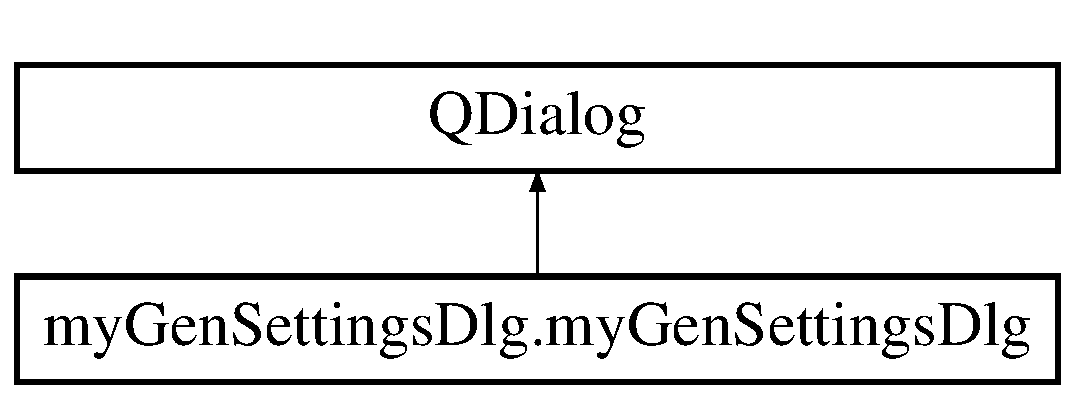
\includegraphics[height=2.000000cm]{classmyGenSettingsDlg_1_1myGenSettingsDlg}
\end{center}
\end{figure}
\subsection*{Public Member Functions}
\begin{DoxyCompactItemize}
\item 
\hypertarget{classmyGenSettingsDlg_1_1myGenSettingsDlg_a3448925fd65dc436f29ba58f0c7e9deb}{def {\bfseries \-\_\-\-\_\-init\-\_\-\-\_\-}}\label{classmyGenSettingsDlg_1_1myGenSettingsDlg_a3448925fd65dc436f29ba58f0c7e9deb}

\item 
\hypertarget{classmyGenSettingsDlg_1_1myGenSettingsDlg_a40a26f42e44ecf94a5b89092ab317175}{def {\bfseries set\-Initial\-Vals}}\label{classmyGenSettingsDlg_1_1myGenSettingsDlg_a40a26f42e44ecf94a5b89092ab317175}

\item 
\hypertarget{classmyGenSettingsDlg_1_1myGenSettingsDlg_a5dd7698aba9583809754a31fc8238672}{def {\bfseries make\-Str}}\label{classmyGenSettingsDlg_1_1myGenSettingsDlg_a5dd7698aba9583809754a31fc8238672}

\item 
\hypertarget{classmyGenSettingsDlg_1_1myGenSettingsDlg_a4f80cb0ec2b9ae4d4fc1ce406007d791}{def {\bfseries get\-Vals}}\label{classmyGenSettingsDlg_1_1myGenSettingsDlg_a4f80cb0ec2b9ae4d4fc1ce406007d791}

\item 
\hypertarget{classmyGenSettingsDlg_1_1myGenSettingsDlg_aa06ce3e18bd1fdbfc32f72ae686f4813}{def {\bfseries set\-Arr}}\label{classmyGenSettingsDlg_1_1myGenSettingsDlg_aa06ce3e18bd1fdbfc32f72ae686f4813}

\item 
\hypertarget{classmyGenSettingsDlg_1_1myGenSettingsDlg_a03b1388aa3a51707339623b639675e15}{def {\bfseries cancel\-This}}\label{classmyGenSettingsDlg_1_1myGenSettingsDlg_a03b1388aa3a51707339623b639675e15}

\item 
\hypertarget{classmyGenSettingsDlg_1_1myGenSettingsDlg_a14c60bbaa985b6bceea42afe3fb1a44c}{def {\bfseries close\-Up}}\label{classmyGenSettingsDlg_1_1myGenSettingsDlg_a14c60bbaa985b6bceea42afe3fb1a44c}

\end{DoxyCompactItemize}
\subsection*{Public Attributes}
\begin{DoxyCompactItemize}
\item 
\hypertarget{classmyGenSettingsDlg_1_1myGenSettingsDlg_a7273bd37d323cb99b1babfe474fb0794}{{\bfseries ui}}\label{classmyGenSettingsDlg_1_1myGenSettingsDlg_a7273bd37d323cb99b1babfe474fb0794}

\item 
\hypertarget{classmyGenSettingsDlg_1_1myGenSettingsDlg_abb00b15bb0a18384e61e828dd8df30b7}{{\bfseries arr}}\label{classmyGenSettingsDlg_1_1myGenSettingsDlg_abb00b15bb0a18384e61e828dd8df30b7}

\item 
\hypertarget{classmyGenSettingsDlg_1_1myGenSettingsDlg_a0a6c727a9bd3bc9a5eccb189f58e0a6a}{{\bfseries status}}\label{classmyGenSettingsDlg_1_1myGenSettingsDlg_a0a6c727a9bd3bc9a5eccb189f58e0a6a}

\end{DoxyCompactItemize}
\subsection*{Static Public Attributes}
\begin{DoxyCompactItemize}
\item 
\hypertarget{classmyGenSettingsDlg_1_1myGenSettingsDlg_af1f09c584de47bbe2a149f514d48bc9c}{{\bfseries second\-Flag} = False}\label{classmyGenSettingsDlg_1_1myGenSettingsDlg_af1f09c584de47bbe2a149f514d48bc9c}

\item 
\hypertarget{classmyGenSettingsDlg_1_1myGenSettingsDlg_ac6e0f33c3d90c70cfb468c892557316a}{string {\bfseries infile} = \char`\"{}\char`\"{}}\label{classmyGenSettingsDlg_1_1myGenSettingsDlg_ac6e0f33c3d90c70cfb468c892557316a}

\item 
\hypertarget{classmyGenSettingsDlg_1_1myGenSettingsDlg_a9f34f21544d7598a99027a2d828e2c36}{int {\bfseries status} = 0}\label{classmyGenSettingsDlg_1_1myGenSettingsDlg_a9f34f21544d7598a99027a2d828e2c36}

\end{DoxyCompactItemize}


The documentation for this class was generated from the following file\-:\begin{DoxyCompactItemize}
\item 
/home/harold/workdir/atrex/\-Software/my\-Gen\-Settings\-Dlg.\-py\end{DoxyCompactItemize}

\hypertarget{classmyImage_1_1myImage}{\section{my\-Image.\-my\-Image Class Reference}
\label{classmyImage_1_1myImage}\index{my\-Image.\-my\-Image@{my\-Image.\-my\-Image}}
}
\subsection*{Public Member Functions}
\begin{DoxyCompactItemize}
\item 
\hypertarget{classmyImage_1_1myImage_a204047031d17ac62cf6dc595185d4b32}{def {\bfseries \-\_\-\-\_\-init\-\_\-\-\_\-}}\label{classmyImage_1_1myImage_a204047031d17ac62cf6dc595185d4b32}

\item 
\hypertarget{classmyImage_1_1myImage_a768c74be8efacd379b8cd320a085f999}{def {\bfseries set\-Series\-Flag}}\label{classmyImage_1_1myImage_a768c74be8efacd379b8cd320a085f999}

\item 
\hypertarget{classmyImage_1_1myImage_ad204cb41e7063c2c059be7edcb869fde}{def {\bfseries read\-Tiff\-Raw}}\label{classmyImage_1_1myImage_ad204cb41e7063c2c059be7edcb869fde}

\item 
\hypertarget{classmyImage_1_1myImage_a9b2b7ca12028fc3c486ba1596986d200}{def {\bfseries read\-Tiff}}\label{classmyImage_1_1myImage_a9b2b7ca12028fc3c486ba1596986d200}

\item 
\hypertarget{classmyImage_1_1myImage_a917e8be7bd24e011ec4fdb6b5e302a76}{def {\bfseries read\-H\-D\-F5}}\label{classmyImage_1_1myImage_a917e8be7bd24e011ec4fdb6b5e302a76}

\item 
\hypertarget{classmyImage_1_1myImage_abf9d2037186dd54cfc3f98d3a14ec7b2}{def {\bfseries read\-Text}}\label{classmyImage_1_1myImage_abf9d2037186dd54cfc3f98d3a14ec7b2}

\item 
\hypertarget{classmyImage_1_1myImage_ab635848195e04c8ee65750cd608050d5}{def {\bfseries set\-Fit\-Params}}\label{classmyImage_1_1myImage_ab635848195e04c8ee65750cd608050d5}

\item 
\hypertarget{classmyImage_1_1myImage_abafcf585a9411b11a26e43db2f840d89}{def {\bfseries set\-B\-S2}}\label{classmyImage_1_1myImage_abafcf585a9411b11a26e43db2f840d89}

\item 
def \hyperlink{classmyImage_1_1myImage_a05b5ee527dc7b0fb413a85b576a55878}{calculate\-\_\-local\-\_\-background}
\item 
\hypertarget{classmyImage_1_1myImage_a78f609d68b1e6e2ba6da84435d4354d4}{def {\bfseries smooth2}}\label{classmyImage_1_1myImage_a78f609d68b1e6e2ba6da84435d4354d4}

\item 
\hypertarget{classmyImage_1_1myImage_a2047e3373cb462f4b7da16551a106cb2}{def {\bfseries smooth\-Gauss}}\label{classmyImage_1_1myImage_a2047e3373cb462f4b7da16551a106cb2}

\item 
\hypertarget{classmyImage_1_1myImage_a288af89bccb1aeb479746201f5f349e0}{def {\bfseries estimate\-\_\-local\-\_\-background}}\label{classmyImage_1_1myImage_a288af89bccb1aeb479746201f5f349e0}

\item 
\hypertarget{classmyImage_1_1myImage_a7d27a9c7a1708eedb66c5d2df6d83793}{def {\bfseries grow\-\_\-peak}}\label{classmyImage_1_1myImage_a7d27a9c7a1708eedb66c5d2df6d83793}

\item 
\hypertarget{classmyImage_1_1myImage_a50a355a2d27f7f62347eb2ecda76cc7f}{def {\bfseries search\-\_\-for\-\_\-peaks\-\_\-arr}}\label{classmyImage_1_1myImage_a50a355a2d27f7f62347eb2ecda76cc7f}

\item 
\hypertarget{classmyImage_1_1myImage_a947569b9e4f7e027e178961c8593e56d}{def {\bfseries search\-\_\-for\-\_\-peaks}}\label{classmyImage_1_1myImage_a947569b9e4f7e027e178961c8593e56d}

\item 
\hypertarget{classmyImage_1_1myImage_adea2c14e68b72ffd6c49a9eb82cdefed}{def {\bfseries fit\-All\-Peaks}}\label{classmyImage_1_1myImage_adea2c14e68b72ffd6c49a9eb82cdefed}

\item 
\hypertarget{classmyImage_1_1myImage_a91c0b54e9f84946cdb34226f43d9f522}{def {\bfseries fit\-Peaks}}\label{classmyImage_1_1myImage_a91c0b54e9f84946cdb34226f43d9f522}

\item 
\hypertarget{classmyImage_1_1myImage_a173a802a68d53a2e6ab9976c00798f22}{def {\bfseries fit\-Peak}}\label{classmyImage_1_1myImage_a173a802a68d53a2e6ab9976c00798f22}

\item 
\hypertarget{classmyImage_1_1myImage_ac7d39571b3e508c285ea29391e81d83d}{def {\bfseries apply\-Mask}}\label{classmyImage_1_1myImage_ac7d39571b3e508c285ea29391e81d83d}

\item 
\hypertarget{classmyImage_1_1myImage_a009bddf285b30ea0d051f171ae08c699}{def {\bfseries two\-\_\-profile\-\_\-fitting}}\label{classmyImage_1_1myImage_a009bddf285b30ea0d051f171ae08c699}

\item 
\hypertarget{classmyImage_1_1myImage_a3e4438a5b3c72363d2754fbdb3cb5fc2}{def {\bfseries one\-\_\-profile\-\_\-fitting}}\label{classmyImage_1_1myImage_a3e4438a5b3c72363d2754fbdb3cb5fc2}

\item 
\hypertarget{classmyImage_1_1myImage_a6b3c5806c372f9e2a2e268db30028725}{def {\bfseries get\-Zoom\-Im}}\label{classmyImage_1_1myImage_a6b3c5806c372f9e2a2e268db30028725}

\item 
\hypertarget{classmyImage_1_1myImage_a6d3a40f22167549a6c6d68d61c34fe88}{def {\bfseries integrate}}\label{classmyImage_1_1myImage_a6d3a40f22167549a6c6d68d61c34fe88}

\item 
\hypertarget{classmyImage_1_1myImage_a7f239b15b61b6564c51b279b337c04a6}{def {\bfseries cake}}\label{classmyImage_1_1myImage_a7f239b15b61b6564c51b279b337c04a6}

\item 
\hypertarget{classmyImage_1_1myImage_a856322994a555fbc012cffd887621d49}{def {\bfseries gauss\-\_\-kernel}}\label{classmyImage_1_1myImage_a856322994a555fbc012cffd887621d49}

\end{DoxyCompactItemize}
\subsection*{Public Attributes}
\begin{DoxyCompactItemize}
\item 
\hypertarget{classmyImage_1_1myImage_a4b84b1393353cf07c3f6a8e876b1bd1e}{{\bfseries Calc\-Theta}}\label{classmyImage_1_1myImage_a4b84b1393353cf07c3f6a8e876b1bd1e}

\item 
\hypertarget{classmyImage_1_1myImage_aa0fefced4570ecbb019e988256a92af0}{{\bfseries loc\-Bcgr}}\label{classmyImage_1_1myImage_aa0fefced4570ecbb019e988256a92af0}

\item 
\hypertarget{classmyImage_1_1myImage_a7185c12e7e3dd7cd5855666f36e08bac}{{\bfseries grad\-Add}}\label{classmyImage_1_1myImage_a7185c12e7e3dd7cd5855666f36e08bac}

\item 
\hypertarget{classmyImage_1_1myImage_a16aea950f266376e528d58844626de3f}{{\bfseries max\-Count}}\label{classmyImage_1_1myImage_a16aea950f266376e528d58844626de3f}

\item 
\hypertarget{classmyImage_1_1myImage_a1bc1ecd6bcba7b02715f99adf9782a2f}{{\bfseries smooth\-Win}}\label{classmyImage_1_1myImage_a1bc1ecd6bcba7b02715f99adf9782a2f}

\item 
\hypertarget{classmyImage_1_1myImage_add1c68f1dd82f1e374ea58177a620d43}{{\bfseries min\-Count}}\label{classmyImage_1_1myImage_add1c68f1dd82f1e374ea58177a620d43}

\item 
\hypertarget{classmyImage_1_1myImage_a547a8aa7edd8e4d9e49e804f610c1a6b}{{\bfseries fit\-Flag}}\label{classmyImage_1_1myImage_a547a8aa7edd8e4d9e49e804f610c1a6b}

\item 
\hypertarget{classmyImage_1_1myImage_a27a025ea4287d51d55ffc3e2f5924dc0}{{\bfseries cur\-Img\-Flag}}\label{classmyImage_1_1myImage_a27a025ea4287d51d55ffc3e2f5924dc0}

\item 
\hypertarget{classmyImage_1_1myImage_a617aeba9d621c3ee6b371d5de03f9d3a}{{\bfseries bs2}}\label{classmyImage_1_1myImage_a617aeba9d621c3ee6b371d5de03f9d3a}

\item 
\hypertarget{classmyImage_1_1myImage_ae621f0bcbbeb1a1c5df305d2ff74854b}{{\bfseries im\-File\-Name}}\label{classmyImage_1_1myImage_ae621f0bcbbeb1a1c5df305d2ff74854b}

\item 
\hypertarget{classmyImage_1_1myImage_ae295dbccaa65f3c6d829c9f551fd1784}{{\bfseries im\-Array\-Size}}\label{classmyImage_1_1myImage_ae295dbccaa65f3c6d829c9f551fd1784}

\item 
\hypertarget{classmyImage_1_1myImage_a3b6b9e69cb643420041fd42acfddfbb3}{{\bfseries im\-Array}}\label{classmyImage_1_1myImage_a3b6b9e69cb643420041fd42acfddfbb3}

\item 
\hypertarget{classmyImage_1_1myImage_a906a618554e161fbe95e24b508ab6e1a}{{\bfseries im\-Array\-\_\-orig}}\label{classmyImage_1_1myImage_a906a618554e161fbe95e24b508ab6e1a}

\item 
\hypertarget{classmyImage_1_1myImage_a7a46de614f68043e9420babac8f2251f}{{\bfseries omega0}}\label{classmyImage_1_1myImage_a7a46de614f68043e9420babac8f2251f}

\item 
\hypertarget{classmyImage_1_1myImage_a48c38f81bb2ec3d332ff80510eef2846}{{\bfseries omega\-R}}\label{classmyImage_1_1myImage_a48c38f81bb2ec3d332ff80510eef2846}

\item 
\hypertarget{classmyImage_1_1myImage_a854752a842ba427ab11635637efd0ea5}{{\bfseries chi}}\label{classmyImage_1_1myImage_a854752a842ba427ab11635637efd0ea5}

\item 
\hypertarget{classmyImage_1_1myImage_acb013415d500b36477f96e19ed9cc3ab}{{\bfseries detector}}\label{classmyImage_1_1myImage_acb013415d500b36477f96e19ed9cc3ab}

\item 
\hypertarget{classmyImage_1_1myImage_a88013815f7b3f0a5dcd02bca7ff96b41}{{\bfseries exposure\-T}}\label{classmyImage_1_1myImage_a88013815f7b3f0a5dcd02bca7ff96b41}

\item 
\hypertarget{classmyImage_1_1myImage_a0635beb1641a5a1b7c1045dbd01bf4c4}{{\bfseries avg2tth}}\label{classmyImage_1_1myImage_a0635beb1641a5a1b7c1045dbd01bf4c4}

\item 
\hypertarget{classmyImage_1_1myImage_a979ecbe45f1292ab528cefd83baad4c4}{{\bfseries tthetabin}}\label{classmyImage_1_1myImage_a979ecbe45f1292ab528cefd83baad4c4}

\item 
\hypertarget{classmyImage_1_1myImage_aeaf615c8bded2e97661cfc47db6d0371}{{\bfseries nbins\-Az}}\label{classmyImage_1_1myImage_aeaf615c8bded2e97661cfc47db6d0371}

\item 
\hypertarget{classmyImage_1_1myImage_a722eda5ce89e24cebc89da923364fb0b}{{\bfseries nbins\-Tth}}\label{classmyImage_1_1myImage_a722eda5ce89e24cebc89da923364fb0b}

\item 
\hypertarget{classmyImage_1_1myImage_a5320605221fb992b852046a41947a458}{{\bfseries cake\-Arr}}\label{classmyImage_1_1myImage_a5320605221fb992b852046a41947a458}

\item 
\hypertarget{classmyImage_1_1myImage_a24f984efb2d87cb956bcce7c8a626a41}{{\bfseries cake\-Params}}\label{classmyImage_1_1myImage_a24f984efb2d87cb956bcce7c8a626a41}

\end{DoxyCompactItemize}
\subsection*{Static Public Attributes}
\begin{DoxyCompactItemize}
\item 
\hypertarget{classmyImage_1_1myImage_ab9dbc690933fa5ba491388ceb1e214a0}{string {\bfseries omega0} = ''}\label{classmyImage_1_1myImage_ab9dbc690933fa5ba491388ceb1e214a0}

\item 
\hypertarget{classmyImage_1_1myImage_ab739c7aa096b85bcdcce37dcb3c5c53c}{string {\bfseries omega\-R} = ''}\label{classmyImage_1_1myImage_ab739c7aa096b85bcdcce37dcb3c5c53c}

\item 
\hypertarget{classmyImage_1_1myImage_ae0a5c8578f1aa53e8f53b522c5cf29a5}{string {\bfseries chi} = ''}\label{classmyImage_1_1myImage_ae0a5c8578f1aa53e8f53b522c5cf29a5}

\item 
\hypertarget{classmyImage_1_1myImage_aea69242e33fa2cc728dbfd434d44f3ed}{string {\bfseries exposure\-T} = ''}\label{classmyImage_1_1myImage_aea69242e33fa2cc728dbfd434d44f3ed}

\item 
\hypertarget{classmyImage_1_1myImage_a0d210dc06284b429870e79968bbcbf96}{string {\bfseries detector} = ''}\label{classmyImage_1_1myImage_a0d210dc06284b429870e79968bbcbf96}

\item 
\hypertarget{classmyImage_1_1myImage_affbde3eed0befed324a6abf5d8224553}{list {\bfseries im\-Array\-Size} = \mbox{[}0,0\mbox{]}}\label{classmyImage_1_1myImage_affbde3eed0befed324a6abf5d8224553}

\item 
\hypertarget{classmyImage_1_1myImage_a2413505e2530877553bf1c15fd5177ba}{string {\bfseries im\-File\-Name} = ''}\label{classmyImage_1_1myImage_a2413505e2530877553bf1c15fd5177ba}

\end{DoxyCompactItemize}


\subsection{Member Function Documentation}
\hypertarget{classmyImage_1_1myImage_a05b5ee527dc7b0fb413a85b576a55878}{\index{my\-Image\-::my\-Image@{my\-Image\-::my\-Image}!calculate\-\_\-local\-\_\-background@{calculate\-\_\-local\-\_\-background}}
\index{calculate\-\_\-local\-\_\-background@{calculate\-\_\-local\-\_\-background}!myImage::myImage@{my\-Image\-::my\-Image}}
\subsubsection[{calculate\-\_\-local\-\_\-background}]{\setlength{\rightskip}{0pt plus 5cm}def my\-Image.\-my\-Image.\-calculate\-\_\-local\-\_\-background (
\begin{DoxyParamCaption}
\item[{}]{self, }
\item[{}]{corners, }
\item[{}]{nregions = {\ttfamily 50}}
\end{DoxyParamCaption}
)}}\label{classmyImage_1_1myImage_a05b5ee527dc7b0fb413a85b576a55878}
\begin{DoxyVerb}calculates the local background using median value in rectangular regions
\end{DoxyVerb}
 

The documentation for this class was generated from the following file\-:\begin{DoxyCompactItemize}
\item 
/home/harold/workdir/atrex/\-Software/my\-Image.\-py\end{DoxyCompactItemize}

\hypertarget{classmyImDisplay_1_1myImDisplay}{\section{my\-Im\-Display.\-my\-Im\-Display Class Reference}
\label{classmyImDisplay_1_1myImDisplay}\index{my\-Im\-Display.\-my\-Im\-Display@{my\-Im\-Display.\-my\-Im\-Display}}
}
Inheritance diagram for my\-Im\-Display.\-my\-Im\-Display\-:\begin{figure}[H]
\begin{center}
\leavevmode
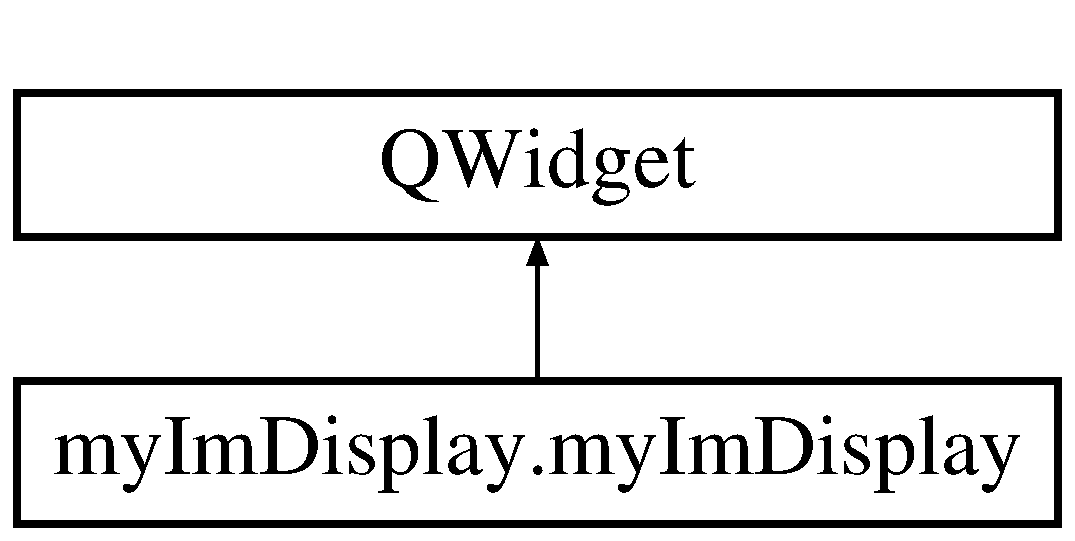
\includegraphics[height=2.000000cm]{classmyImDisplay_1_1myImDisplay}
\end{center}
\end{figure}
\subsection*{Public Member Functions}
\begin{DoxyCompactItemize}
\item 
\hypertarget{classmyImDisplay_1_1myImDisplay_ac84ff467e290df4e4ab1d4c65d4267f5}{def {\bfseries \-\_\-\-\_\-init\-\_\-\-\_\-}}\label{classmyImDisplay_1_1myImDisplay_ac84ff467e290df4e4ab1d4c65d4267f5}

\item 
\hypertarget{classmyImDisplay_1_1myImDisplay_ab744180f478698e143f8470430f1d192}{def {\bfseries set\-Peak\-Box\-Size}}\label{classmyImDisplay_1_1myImDisplay_ab744180f478698e143f8470430f1d192}

\item 
\hypertarget{classmyImDisplay_1_1myImDisplay_ab09a20ba11a398d503273b7f422c2644}{def {\bfseries set\-Cake\-Image}}\label{classmyImDisplay_1_1myImDisplay_ab09a20ba11a398d503273b7f422c2644}

\item 
\hypertarget{classmyImDisplay_1_1myImDisplay_a3352c4bc953e0a9f393d08871e5d1c31}{def {\bfseries context\-Menu\-Kickoff}}\label{classmyImDisplay_1_1myImDisplay_a3352c4bc953e0a9f393d08871e5d1c31}

\item 
\hypertarget{classmyImDisplay_1_1myImDisplay_a8093fb201222b74f57c27297f1e6d84a}{def {\bfseries zoom\-On}}\label{classmyImDisplay_1_1myImDisplay_a8093fb201222b74f57c27297f1e6d84a}

\item 
\hypertarget{classmyImDisplay_1_1myImDisplay_ae60543e0ec298c4a15e385f11091b675}{def {\bfseries peak\-Add}}\label{classmyImDisplay_1_1myImDisplay_ae60543e0ec298c4a15e385f11091b675}

\item 
\hypertarget{classmyImDisplay_1_1myImDisplay_a29d16cbb8188fd3f8c15fa6014b231e8}{def {\bfseries select\-On}}\label{classmyImDisplay_1_1myImDisplay_a29d16cbb8188fd3f8c15fa6014b231e8}

\item 
\hypertarget{classmyImDisplay_1_1myImDisplay_a6f9207ced879b40fb101f1994ba71eef}{def {\bfseries unselect\-On}}\label{classmyImDisplay_1_1myImDisplay_a6f9207ced879b40fb101f1994ba71eef}

\item 
\hypertarget{classmyImDisplay_1_1myImDisplay_a7411fd0ab99914cd633c779309de1d07}{def {\bfseries mask\-On}}\label{classmyImDisplay_1_1myImDisplay_a7411fd0ab99914cd633c779309de1d07}

\item 
\hypertarget{classmyImDisplay_1_1myImDisplay_a30939cb6a115426fc1d37960cbb19297}{def {\bfseries unmask\-On}}\label{classmyImDisplay_1_1myImDisplay_a30939cb6a115426fc1d37960cbb19297}

\item 
\hypertarget{classmyImDisplay_1_1myImDisplay_acd33a2cd440fea030b809b07d9356e10}{def {\bfseries set\-Min\-Max}}\label{classmyImDisplay_1_1myImDisplay_acd33a2cd440fea030b809b07d9356e10}

\item 
\hypertarget{classmyImDisplay_1_1myImDisplay_a68c47131be6412075f42b0b1725f9964}{def {\bfseries set\-Zm\-Rect}}\label{classmyImDisplay_1_1myImDisplay_a68c47131be6412075f42b0b1725f9964}

\item 
\hypertarget{classmyImDisplay_1_1myImDisplay_a05a3f0227ee151a60323a4c1a98fb48f}{def {\bfseries calc\-Histo}}\label{classmyImDisplay_1_1myImDisplay_a05a3f0227ee151a60323a4c1a98fb48f}

\item 
\hypertarget{classmyImDisplay_1_1myImDisplay_a54c41ffb58933e7d11d44267fd893330}{def {\bfseries write\-Q\-Image}}\label{classmyImDisplay_1_1myImDisplay_a54c41ffb58933e7d11d44267fd893330}

\item 
\hypertarget{classmyImDisplay_1_1myImDisplay_aaf7a8e0381472923f2b0c40ab8b2b842}{def {\bfseries write\-Q\-Image\-\_\-lut}}\label{classmyImDisplay_1_1myImDisplay_aaf7a8e0381472923f2b0c40ab8b2b842}

\item 
\hypertarget{classmyImDisplay_1_1myImDisplay_a4547adad958556b811c45e2a4b89308e}{def {\bfseries set\-L\-U\-T}}\label{classmyImDisplay_1_1myImDisplay_a4547adad958556b811c45e2a4b89308e}

\item 
\hypertarget{classmyImDisplay_1_1myImDisplay_a5085f34b80cfdd3b00758515585a0fbf}{def \hyperlink{classmyImDisplay_1_1myImDisplay_a5085f34b80cfdd3b00758515585a0fbf}{mouse\-Release\-Event}}\label{classmyImDisplay_1_1myImDisplay_a5085f34b80cfdd3b00758515585a0fbf}

\begin{DoxyCompactList}\small\item\em Mouse Functions. \end{DoxyCompactList}\item 
\hypertarget{classmyImDisplay_1_1myImDisplay_aff9f38dbac669da47bfb829837b8b74b}{def {\bfseries mouse\-Press\-Event}}\label{classmyImDisplay_1_1myImDisplay_aff9f38dbac669da47bfb829837b8b74b}

\item 
\hypertarget{classmyImDisplay_1_1myImDisplay_ac65f590d7f74cf11fc8dcb2dfa3eb669}{def {\bfseries mouse\-Move\-Event}}\label{classmyImDisplay_1_1myImDisplay_ac65f590d7f74cf11fc8dcb2dfa3eb669}

\item 
\hypertarget{classmyImDisplay_1_1myImDisplay_a5ef52021cb9f418ed66ef0d8ba064430}{def {\bfseries peak\-Find}}\label{classmyImDisplay_1_1myImDisplay_a5ef52021cb9f418ed66ef0d8ba064430}

\item 
\hypertarget{classmyImDisplay_1_1myImDisplay_a4408bd12e5abc5fb4f6e82bec3bb22c8}{def {\bfseries set\-Peaks}}\label{classmyImDisplay_1_1myImDisplay_a4408bd12e5abc5fb4f6e82bec3bb22c8}

\item 
\hypertarget{classmyImDisplay_1_1myImDisplay_a4c809a5912d974d2d819b5b1937638cd}{def {\bfseries paint\-Event}}\label{classmyImDisplay_1_1myImDisplay_a4c809a5912d974d2d819b5b1937638cd}

\item 
\hypertarget{classmyImDisplay_1_1myImDisplay_a6bb6690d1ba6d5087ca3520d7095a625}{def {\bfseries apply\-Mask}}\label{classmyImDisplay_1_1myImDisplay_a6bb6690d1ba6d5087ca3520d7095a625}

\item 
\hypertarget{classmyImDisplay_1_1myImDisplay_ab0ad3b819095b75f6f02df31428d7e03}{def {\bfseries apply\-Mask\-To\-Array}}\label{classmyImDisplay_1_1myImDisplay_ab0ad3b819095b75f6f02df31428d7e03}

\item 
\hypertarget{classmyImDisplay_1_1myImDisplay_a9dbb51a8119e4699a1fa0fd757bb1e09}{def {\bfseries set\-Calibration\-Marks}}\label{classmyImDisplay_1_1myImDisplay_a9dbb51a8119e4699a1fa0fd757bb1e09}

\item 
\hypertarget{classmyImDisplay_1_1myImDisplay_ab0ad940e09349167e907fccb728efbe0}{def {\bfseries set\-Prox\-Points}}\label{classmyImDisplay_1_1myImDisplay_ab0ad940e09349167e907fccb728efbe0}

\item 
\hypertarget{classmyImDisplay_1_1myImDisplay_a664b4ec105bbea3104ece30e58fd12f0}{def {\bfseries set\-Ring\-Points}}\label{classmyImDisplay_1_1myImDisplay_a664b4ec105bbea3104ece30e58fd12f0}

\end{DoxyCompactItemize}
\subsection*{Public Attributes}
\begin{DoxyCompactItemize}
\item 
\hypertarget{classmyImDisplay_1_1myImDisplay_a388bff72546f1d6fac13520142b77095}{{\bfseries cal\-Points\-Flag}}\label{classmyImDisplay_1_1myImDisplay_a388bff72546f1d6fac13520142b77095}

\item 
\hypertarget{classmyImDisplay_1_1myImDisplay_ae2050cee691f881f69d1bc9caa02b8f5}{{\bfseries cal\-Points}}\label{classmyImDisplay_1_1myImDisplay_ae2050cee691f881f69d1bc9caa02b8f5}

\item 
\hypertarget{classmyImDisplay_1_1myImDisplay_acc86c3f609b093d1dab093d5d458db1c}{{\bfseries prox\-Points}}\label{classmyImDisplay_1_1myImDisplay_acc86c3f609b093d1dab093d5d458db1c}

\item 
\hypertarget{classmyImDisplay_1_1myImDisplay_aa0bc29d37aa4ceea5a1b6e73bb1b5b2a}{{\bfseries prox\-Points\-F}}\label{classmyImDisplay_1_1myImDisplay_aa0bc29d37aa4ceea5a1b6e73bb1b5b2a}

\item 
\hypertarget{classmyImDisplay_1_1myImDisplay_ada88e83e5af43af9c5887368b6c7ea55}{{\bfseries n\-Rings}}\label{classmyImDisplay_1_1myImDisplay_ada88e83e5af43af9c5887368b6c7ea55}

\item 
\hypertarget{classmyImDisplay_1_1myImDisplay_aab0a908d56ebacba2362d56cf533db7b}{{\bfseries pts\-Per\-Ring}}\label{classmyImDisplay_1_1myImDisplay_aab0a908d56ebacba2362d56cf533db7b}

\item 
\hypertarget{classmyImDisplay_1_1myImDisplay_a43cb9bc23b346f4b1d916ff61f11184c}{{\bfseries rings\-X}}\label{classmyImDisplay_1_1myImDisplay_a43cb9bc23b346f4b1d916ff61f11184c}

\item 
\hypertarget{classmyImDisplay_1_1myImDisplay_a7b16faa290f90ab6ffa95782b374f88b}{{\bfseries rings\-Y}}\label{classmyImDisplay_1_1myImDisplay_a7b16faa290f90ab6ffa95782b374f88b}

\item 
\hypertarget{classmyImDisplay_1_1myImDisplay_abe157e3a38400a86b33ed3ad78aee75d}{{\bfseries peak\-Box\-Size}}\label{classmyImDisplay_1_1myImDisplay_abe157e3a38400a86b33ed3ad78aee75d}

\item 
\hypertarget{classmyImDisplay_1_1myImDisplay_a73cfa3418c302cd63b7583b44b9c3b98}{{\bfseries disp\-Min}}\label{classmyImDisplay_1_1myImDisplay_a73cfa3418c302cd63b7583b44b9c3b98}

\item 
\hypertarget{classmyImDisplay_1_1myImDisplay_a9472fc9988a7d5b4b3d26555eff36629}{{\bfseries disp\-Max}}\label{classmyImDisplay_1_1myImDisplay_a9472fc9988a7d5b4b3d26555eff36629}

\item 
\hypertarget{classmyImDisplay_1_1myImDisplay_a2fef2a841184ea3d06026f30fedb9c68}{{\bfseries zm\-Rect}}\label{classmyImDisplay_1_1myImDisplay_a2fef2a841184ea3d06026f30fedb9c68}

\item 
\hypertarget{classmyImDisplay_1_1myImDisplay_ad52cc4c765b66c9200b3d3fbf8415170}{{\bfseries zm\-Size}}\label{classmyImDisplay_1_1myImDisplay_ad52cc4c765b66c9200b3d3fbf8415170}

\item 
\hypertarget{classmyImDisplay_1_1myImDisplay_a6ae8912d4d04b0a655e1a01fd8070ff6}{{\bfseries ind\-\_\-5}}\label{classmyImDisplay_1_1myImDisplay_a6ae8912d4d04b0a655e1a01fd8070ff6}

\item 
\hypertarget{classmyImDisplay_1_1myImDisplay_a4d83de595869c13b63e303709bc188a7}{{\bfseries ind\-\_\-95}}\label{classmyImDisplay_1_1myImDisplay_a4d83de595869c13b63e303709bc188a7}

\item 
\hypertarget{classmyImDisplay_1_1myImDisplay_a781283f5accbbaf7562ef6c4a85b662c}{{\bfseries xsize}}\label{classmyImDisplay_1_1myImDisplay_a781283f5accbbaf7562ef6c4a85b662c}

\item 
\hypertarget{classmyImDisplay_1_1myImDisplay_acd126c9a2504bff9bc339acc8f4160d4}{{\bfseries ysize}}\label{classmyImDisplay_1_1myImDisplay_acd126c9a2504bff9bc339acc8f4160d4}

\item 
\hypertarget{classmyImDisplay_1_1myImDisplay_ad82dd773b3509d7c4d283654bc2b22fe}{{\bfseries fulldata}}\label{classmyImDisplay_1_1myImDisplay_ad82dd773b3509d7c4d283654bc2b22fe}

\item 
\hypertarget{classmyImDisplay_1_1myImDisplay_a3643bcc46e320625be4b0a16a366398b}{{\bfseries max}}\label{classmyImDisplay_1_1myImDisplay_a3643bcc46e320625be4b0a16a366398b}

\item 
\hypertarget{classmyImDisplay_1_1myImDisplay_a44e480bf21d1b2f540d95b03d0e41678}{{\bfseries min}}\label{classmyImDisplay_1_1myImDisplay_a44e480bf21d1b2f540d95b03d0e41678}

\item 
\hypertarget{classmyImDisplay_1_1myImDisplay_a60a3651bd482b77f17fd9758418576a6}{{\bfseries scale}}\label{classmyImDisplay_1_1myImDisplay_a60a3651bd482b77f17fd9758418576a6}

\item 
\hypertarget{classmyImDisplay_1_1myImDisplay_a0a4c2d42cb88a1ffcc46de46f97298df}{{\bfseries pscale}}\label{classmyImDisplay_1_1myImDisplay_a0a4c2d42cb88a1ffcc46de46f97298df}

\item 
\hypertarget{classmyImDisplay_1_1myImDisplay_a4aaf1f57b9b82bc1fc8baa8bbb178222}{{\bfseries qimage}}\label{classmyImDisplay_1_1myImDisplay_a4aaf1f57b9b82bc1fc8baa8bbb178222}

\item 
\hypertarget{classmyImDisplay_1_1myImDisplay_a9746a399ab1bed5e1dd795f5996cc242}{{\bfseries load\-Image}}\label{classmyImDisplay_1_1myImDisplay_a9746a399ab1bed5e1dd795f5996cc242}

\item 
\hypertarget{classmyImDisplay_1_1myImDisplay_a9aca945926bdc3f037ba0cc3b155b1a8}{{\bfseries zm\-Fac}}\label{classmyImDisplay_1_1myImDisplay_a9aca945926bdc3f037ba0cc3b155b1a8}

\item 
\hypertarget{classmyImDisplay_1_1myImDisplay_a9e8a54943407a7cce248d03f5b62741a}{{\bfseries imdata}}\label{classmyImDisplay_1_1myImDisplay_a9e8a54943407a7cce248d03f5b62741a}

\item 
\hypertarget{classmyImDisplay_1_1myImDisplay_aa82904a08c5b57df3520dfb0496ce1ba}{{\bfseries rgb\-\_\-lut}}\label{classmyImDisplay_1_1myImDisplay_aa82904a08c5b57df3520dfb0496ce1ba}

\item 
\hypertarget{classmyImDisplay_1_1myImDisplay_aa8be69b012304960b810c37fc9212abb}{{\bfseries select\-Point\-U\-L}}\label{classmyImDisplay_1_1myImDisplay_aa8be69b012304960b810c37fc9212abb}

\item 
\hypertarget{classmyImDisplay_1_1myImDisplay_a520d206f02a9731fb993705899044d46}{{\bfseries select\-Point\-L\-R}}\label{classmyImDisplay_1_1myImDisplay_a520d206f02a9731fb993705899044d46}

\item 
\hypertarget{classmyImDisplay_1_1myImDisplay_af40bf78fd8315226eedca459d686ca05}{{\bfseries dmax}}\label{classmyImDisplay_1_1myImDisplay_af40bf78fd8315226eedca459d686ca05}

\item 
\hypertarget{classmyImDisplay_1_1myImDisplay_aead7802bb20d7a0d6d7f6f680b1cb7e2}{{\bfseries peaks}}\label{classmyImDisplay_1_1myImDisplay_aead7802bb20d7a0d6d7f6f680b1cb7e2}

\item 
\hypertarget{classmyImDisplay_1_1myImDisplay_afde0c76a92daa96ba2d868fe4ee9a228}{{\bfseries curmask}}\label{classmyImDisplay_1_1myImDisplay_afde0c76a92daa96ba2d868fe4ee9a228}

\end{DoxyCompactItemize}
\subsection*{Static Public Attributes}
\begin{DoxyCompactItemize}
\item 
\hypertarget{classmyImDisplay_1_1myImDisplay_aeaa8491db62f6e99ba83f6fa81dc6d74}{int {\bfseries load\-Image} = 0}\label{classmyImDisplay_1_1myImDisplay_aeaa8491db62f6e99ba83f6fa81dc6d74}

\item 
\hypertarget{classmyImDisplay_1_1myImDisplay_aaff409ee4de877ac2f0fcb090e1a5daf}{int {\bfseries disp\-Max} = 65535}\label{classmyImDisplay_1_1myImDisplay_aaff409ee4de877ac2f0fcb090e1a5daf}

\item 
\hypertarget{classmyImDisplay_1_1myImDisplay_a795083e40d9aa9b6e7d4a5d37910e187}{int {\bfseries disp\-Min} = 0}\label{classmyImDisplay_1_1myImDisplay_a795083e40d9aa9b6e7d4a5d37910e187}

\item 
\hypertarget{classmyImDisplay_1_1myImDisplay_a4c5cc84a1c8d090c4c43d8f78b7b4d9f}{int {\bfseries ind\-\_\-5} = 0}\label{classmyImDisplay_1_1myImDisplay_a4c5cc84a1c8d090c4c43d8f78b7b4d9f}

\item 
\hypertarget{classmyImDisplay_1_1myImDisplay_a34f600eea208832c0b785288ccad9fc7}{int {\bfseries zm\-Fac} = 3}\label{classmyImDisplay_1_1myImDisplay_a34f600eea208832c0b785288ccad9fc7}

\item 
\hypertarget{classmyImDisplay_1_1myImDisplay_a02f7742e2c4e540f6585f39c8af717cb}{tuple {\bfseries zm\-Rect} = Qt\-Core.\-Q\-Rect()}\label{classmyImDisplay_1_1myImDisplay_a02f7742e2c4e540f6585f39c8af717cb}

\item 
\hypertarget{classmyImDisplay_1_1myImDisplay_afe92f10aebabc4ab5d3f18a6fea84d75}{tuple {\bfseries cent\-Pt} = Qt\-Core.\-pyqt\-Signal(Qt\-Core.\-Q\-Point)}\label{classmyImDisplay_1_1myImDisplay_afe92f10aebabc4ab5d3f18a6fea84d75}

\item 
\hypertarget{classmyImDisplay_1_1myImDisplay_a52347d8a98f02a25ddc2929a08461909}{tuple {\bfseries add\-Peak\-Signal} = Qt\-Core.\-pyqt\-Signal(Qt\-Core.\-Q\-Point)}\label{classmyImDisplay_1_1myImDisplay_a52347d8a98f02a25ddc2929a08461909}

\item 
\hypertarget{classmyImDisplay_1_1myImDisplay_a9e0436ef995b6fa9769ab1cc004956e4}{tuple {\bfseries select\-Rect\-Signal} = Qt\-Core.\-pyqt\-Signal(Qt\-Core.\-Q\-Rect, bool)}\label{classmyImDisplay_1_1myImDisplay_a9e0436ef995b6fa9769ab1cc004956e4}

\item 
\hypertarget{classmyImDisplay_1_1myImDisplay_aebd7f068977c74a612f0428fe26bf86c}{tuple {\bfseries mask\-Rect\-Signal} = Qt\-Core.\-pyqt\-Signal(Qt\-Core.\-Q\-Rect, bool)}\label{classmyImDisplay_1_1myImDisplay_aebd7f068977c74a612f0428fe26bf86c}

\item 
\hypertarget{classmyImDisplay_1_1myImDisplay_a4c70f21c598d0b670373d09133d09767}{tuple {\bfseries set\-Button\-Mode\-Signal} = Qt\-Core.\-pyqt\-Signal(int)}\label{classmyImDisplay_1_1myImDisplay_a4c70f21c598d0b670373d09133d09767}

\item 
\hypertarget{classmyImDisplay_1_1myImDisplay_a1f5a4286181533164cb3ab70ee622264}{tuple {\bfseries imcoords\-Select\-Signal} = Qt\-Core.\-pyqt\-Signal(list)}\label{classmyImDisplay_1_1myImDisplay_a1f5a4286181533164cb3ab70ee622264}

\item 
\hypertarget{classmyImDisplay_1_1myImDisplay_aed334f8955978445c19ec065984ffdf1}{{\bfseries drag\-Zm} = False}\label{classmyImDisplay_1_1myImDisplay_aed334f8955978445c19ec065984ffdf1}

\item 
\hypertarget{classmyImDisplay_1_1myImDisplay_a1ede5c771d24ccc9bc28d13b9af5aea9}{{\bfseries zoom\-Toggle} = True}\label{classmyImDisplay_1_1myImDisplay_a1ede5c771d24ccc9bc28d13b9af5aea9}

\item 
\hypertarget{classmyImDisplay_1_1myImDisplay_a14cb30b4564e4b042b23f20adbf38c72}{{\bfseries peak\-Toggle} = False}\label{classmyImDisplay_1_1myImDisplay_a14cb30b4564e4b042b23f20adbf38c72}

\item 
\hypertarget{classmyImDisplay_1_1myImDisplay_a233a9c327101136d4cf81d5e47f22f08}{{\bfseries select\-Flag} = False}\label{classmyImDisplay_1_1myImDisplay_a233a9c327101136d4cf81d5e47f22f08}

\item 
\hypertarget{classmyImDisplay_1_1myImDisplay_a31a7d969ae2427fdc98ac41f7097ba5a}{{\bfseries unselect\-Flag} = False}\label{classmyImDisplay_1_1myImDisplay_a31a7d969ae2427fdc98ac41f7097ba5a}

\item 
\hypertarget{classmyImDisplay_1_1myImDisplay_a1afbe7e34027cf61cd59d25b90de33e4}{{\bfseries mask\-Flag} = False}\label{classmyImDisplay_1_1myImDisplay_a1afbe7e34027cf61cd59d25b90de33e4}

\item 
\hypertarget{classmyImDisplay_1_1myImDisplay_a26c93c50e5e9d5f331d3f7c8de49bb73}{{\bfseries unmask\-Flag} = False}\label{classmyImDisplay_1_1myImDisplay_a26c93c50e5e9d5f331d3f7c8de49bb73}

\item 
\hypertarget{classmyImDisplay_1_1myImDisplay_a7b54134bda08a36bc55e9289b3c30b98}{{\bfseries drag\-Flag} = False}\label{classmyImDisplay_1_1myImDisplay_a7b54134bda08a36bc55e9289b3c30b98}

\item 
\hypertarget{classmyImDisplay_1_1myImDisplay_af326649460abba4d85c62746c570961f}{{\bfseries apply\-Mask\-Flag} = False}\label{classmyImDisplay_1_1myImDisplay_af326649460abba4d85c62746c570961f}

\item 
\hypertarget{classmyImDisplay_1_1myImDisplay_a4816a3cbcfb5ef0d5576395ee6c95c59}{tuple {\bfseries rgb\-\_\-lut} = np.\-zeros((3,256), dtype=np.\-uint8)}\label{classmyImDisplay_1_1myImDisplay_a4816a3cbcfb5ef0d5576395ee6c95c59}

\item 
\hypertarget{classmyImDisplay_1_1myImDisplay_a2d68517b926ed8a7ef02dc9053576197}{{\bfseries cake\-Image\-Flag} = False}\label{classmyImDisplay_1_1myImDisplay_a2d68517b926ed8a7ef02dc9053576197}

\item 
\hypertarget{classmyImDisplay_1_1myImDisplay_a0ea2cd018dee5f86a7740c76a7c08014}{int {\bfseries peak\-Box\-Size} = 33}\label{classmyImDisplay_1_1myImDisplay_a0ea2cd018dee5f86a7740c76a7c08014}

\end{DoxyCompactItemize}


The documentation for this class was generated from the following file\-:\begin{DoxyCompactItemize}
\item 
/home/harold/workdir/atrex/\-Software/my\-Im\-Display.\-py\end{DoxyCompactItemize}

\hypertarget{classmyMask_1_1myMask}{\section{my\-Mask.\-my\-Mask Class Reference}
\label{classmyMask_1_1myMask}\index{my\-Mask.\-my\-Mask@{my\-Mask.\-my\-Mask}}
}
Inheritance diagram for my\-Mask.\-my\-Mask\-:\begin{figure}[H]
\begin{center}
\leavevmode
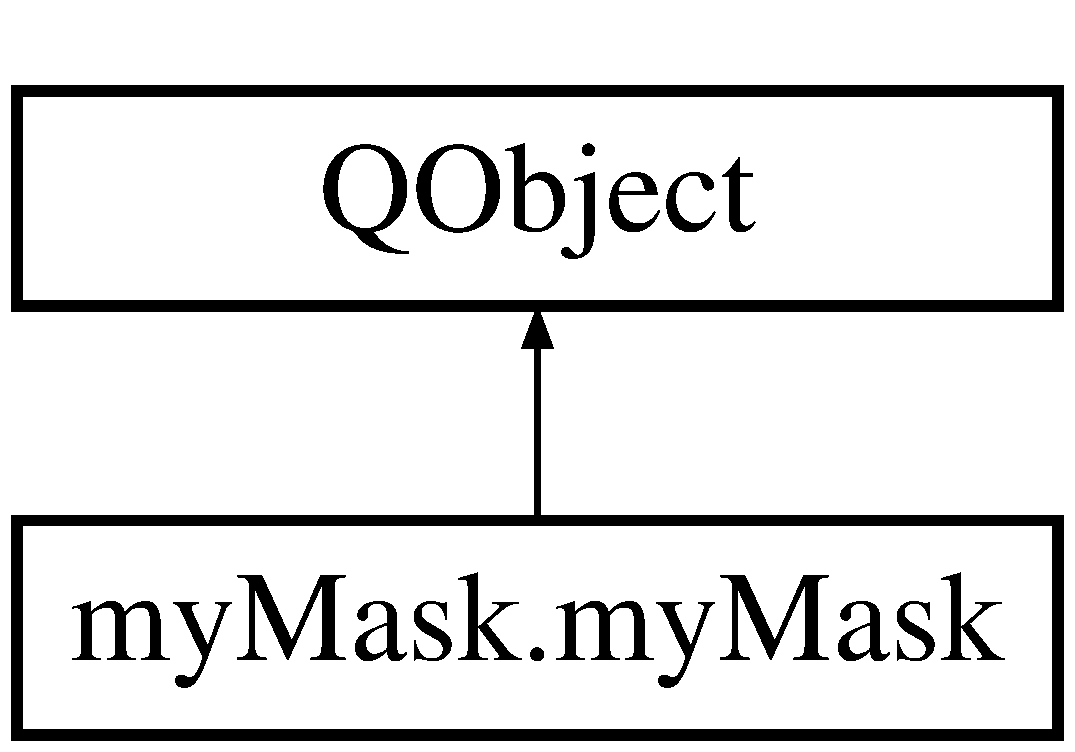
\includegraphics[height=2.000000cm]{classmyMask_1_1myMask}
\end{center}
\end{figure}
\subsection*{Public Member Functions}
\begin{DoxyCompactItemize}
\item 
\hypertarget{classmyMask_1_1myMask_a551d04051af413888f60e9cf74a964fa}{def {\bfseries create\-Mask}}\label{classmyMask_1_1myMask_a551d04051af413888f60e9cf74a964fa}

\item 
\hypertarget{classmyMask_1_1myMask_a0b6e02944d05baf74d75976672b75ba3}{def {\bfseries set\-Mask}}\label{classmyMask_1_1myMask_a0b6e02944d05baf74d75976672b75ba3}

\item 
\hypertarget{classmyMask_1_1myMask_aaa9e1d93e4202095b0c5ffba2d98d53a}{def {\bfseries reset\-Mask}}\label{classmyMask_1_1myMask_aaa9e1d93e4202095b0c5ffba2d98d53a}

\item 
\hypertarget{classmyMask_1_1myMask_a1b17be401eb92b7293e40de411f8b17f}{def {\bfseries save\-To\-File}}\label{classmyMask_1_1myMask_a1b17be401eb92b7293e40de411f8b17f}

\item 
\hypertarget{classmyMask_1_1myMask_aface6241850e7cbc5bc4ae847e936eac}{def {\bfseries read\-Tiff}}\label{classmyMask_1_1myMask_aface6241850e7cbc5bc4ae847e936eac}

\end{DoxyCompactItemize}
\subsection*{Public Attributes}
\begin{DoxyCompactItemize}
\item 
\hypertarget{classmyMask_1_1myMask_abc71579b1017e1a3d98fdca371e771fd}{{\bfseries img}}\label{classmyMask_1_1myMask_abc71579b1017e1a3d98fdca371e771fd}

\item 
\hypertarget{classmyMask_1_1myMask_aec05f7b9af1f9ba5b283f1034f229cdc}{{\bfseries nsamps}}\label{classmyMask_1_1myMask_aec05f7b9af1f9ba5b283f1034f229cdc}

\item 
\hypertarget{classmyMask_1_1myMask_a580ea0a4ec202bbc76ac0ad31b3d9f2b}{{\bfseries nlines}}\label{classmyMask_1_1myMask_a580ea0a4ec202bbc76ac0ad31b3d9f2b}

\item 
\hypertarget{classmyMask_1_1myMask_a70decb30e8747e2688e1840f253f3950}{{\bfseries im\-File\-Name}}\label{classmyMask_1_1myMask_a70decb30e8747e2688e1840f253f3950}

\end{DoxyCompactItemize}
\subsection*{Static Public Attributes}
\begin{DoxyCompactItemize}
\item 
\hypertarget{classmyMask_1_1myMask_a6a94c13fe022b092f42d5be3f3b29fe6}{int {\bfseries nsamps} = 0}\label{classmyMask_1_1myMask_a6a94c13fe022b092f42d5be3f3b29fe6}

\item 
\hypertarget{classmyMask_1_1myMask_a91b9f3c41dd6f0c54860b24069f56ca4}{int {\bfseries nlines} = 0}\label{classmyMask_1_1myMask_a91b9f3c41dd6f0c54860b24069f56ca4}

\end{DoxyCompactItemize}


The documentation for this class was generated from the following file\-:\begin{DoxyCompactItemize}
\item 
/home/harold/workdir/atrex/\-Software/my\-Mask.\-py\end{DoxyCompactItemize}

\hypertarget{classMyOverlayDlg_1_1MyOverlayDlg}{\section{My\-Overlay\-Dlg.\-My\-Overlay\-Dlg Class Reference}
\label{classMyOverlayDlg_1_1MyOverlayDlg}\index{My\-Overlay\-Dlg.\-My\-Overlay\-Dlg@{My\-Overlay\-Dlg.\-My\-Overlay\-Dlg}}
}
Inheritance diagram for My\-Overlay\-Dlg.\-My\-Overlay\-Dlg\-:\begin{figure}[H]
\begin{center}
\leavevmode
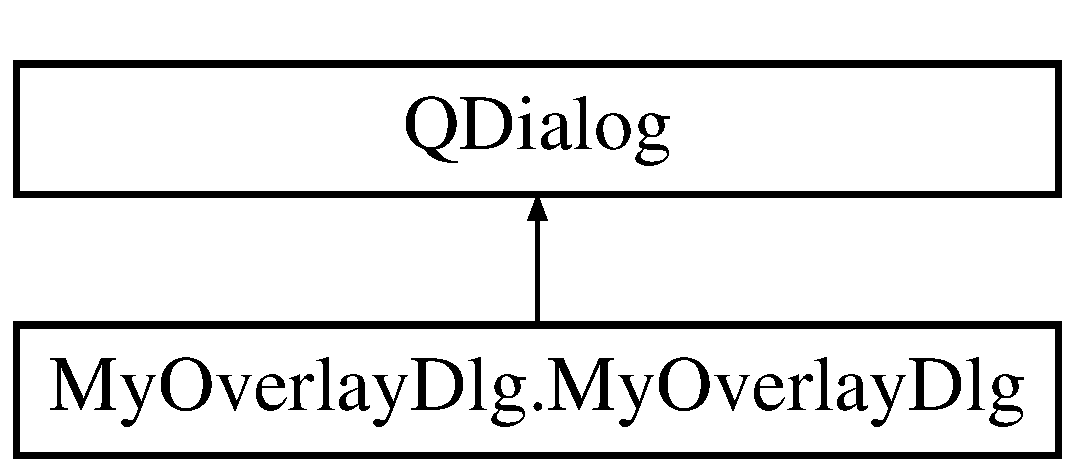
\includegraphics[height=2.000000cm]{classMyOverlayDlg_1_1MyOverlayDlg}
\end{center}
\end{figure}
\subsection*{Public Member Functions}
\begin{DoxyCompactItemize}
\item 
\hypertarget{classMyOverlayDlg_1_1MyOverlayDlg_a836f26cd68556b2b577ba8ebbc36892a}{def {\bfseries \-\_\-\-\_\-init\-\_\-\-\_\-}}\label{classMyOverlayDlg_1_1MyOverlayDlg_a836f26cd68556b2b577ba8ebbc36892a}

\item 
\hypertarget{classMyOverlayDlg_1_1MyOverlayDlg_a30489fcaa881f5dccddcc4782a1fcb2e}{def {\bfseries set\-Params}}\label{classMyOverlayDlg_1_1MyOverlayDlg_a30489fcaa881f5dccddcc4782a1fcb2e}

\item 
\hypertarget{classMyOverlayDlg_1_1MyOverlayDlg_a911fbf22d0431f251fedbc1cc9ceee34}{def {\bfseries accept}}\label{classMyOverlayDlg_1_1MyOverlayDlg_a911fbf22d0431f251fedbc1cc9ceee34}

\item 
\hypertarget{classMyOverlayDlg_1_1MyOverlayDlg_a6b58d65c0fb4398f5187d9636723d4fd}{def {\bfseries browse\-File}}\label{classMyOverlayDlg_1_1MyOverlayDlg_a6b58d65c0fb4398f5187d9636723d4fd}

\end{DoxyCompactItemize}
\subsection*{Public Attributes}
\begin{DoxyCompactItemize}
\item 
\hypertarget{classMyOverlayDlg_1_1MyOverlayDlg_a7d657b769e24e56ee48781d352de441e}{{\bfseries ui}}\label{classMyOverlayDlg_1_1MyOverlayDlg_a7d657b769e24e56ee48781d352de441e}

\item 
\hypertarget{classMyOverlayDlg_1_1MyOverlayDlg_acca8e0275695cf61524525634591381b}{{\bfseries infile}}\label{classMyOverlayDlg_1_1MyOverlayDlg_acca8e0275695cf61524525634591381b}

\end{DoxyCompactItemize}
\subsection*{Static Public Attributes}
\begin{DoxyCompactItemize}
\item 
\hypertarget{classMyOverlayDlg_1_1MyOverlayDlg_a90f6e4408789fb09a8373122658e9dda}{{\bfseries second\-Flag} = False}\label{classMyOverlayDlg_1_1MyOverlayDlg_a90f6e4408789fb09a8373122658e9dda}

\item 
\hypertarget{classMyOverlayDlg_1_1MyOverlayDlg_a9a655828844f2260620132477ff6e2ac}{string {\bfseries infile} = \char`\"{}\char`\"{}}\label{classMyOverlayDlg_1_1MyOverlayDlg_a9a655828844f2260620132477ff6e2ac}

\end{DoxyCompactItemize}


The documentation for this class was generated from the following file\-:\begin{DoxyCompactItemize}
\item 
/home/harold/workdir/atrex/\-Software/My\-Overlay\-Dlg.\-py\end{DoxyCompactItemize}

\hypertarget{classmyPeakTable_1_1myPeak}{\section{my\-Peak\-Table.\-my\-Peak Class Reference}
\label{classmyPeakTable_1_1myPeak}\index{my\-Peak\-Table.\-my\-Peak@{my\-Peak\-Table.\-my\-Peak}}
}
\subsection*{Public Member Functions}
\begin{DoxyCompactItemize}
\item 
\hypertarget{classmyPeakTable_1_1myPeak_a037a4088033f2adfaaa74c7352f70f48}{def {\bfseries \-\_\-\-\_\-init\-\_\-\-\_\-}}\label{classmyPeakTable_1_1myPeak_a037a4088033f2adfaaa74c7352f70f48}

\item 
\hypertarget{classmyPeakTable_1_1myPeak_ad3e58261d15c3ac0e64876ce79e2fb65}{def {\bfseries set\-Detxy}}\label{classmyPeakTable_1_1myPeak_ad3e58261d15c3ac0e64876ce79e2fb65}

\item 
\hypertarget{classmyPeakTable_1_1myPeak_a69641e1873ad1aeb01e9addef6aee25b}{def {\bfseries get\-Detxy}}\label{classmyPeakTable_1_1myPeak_a69641e1873ad1aeb01e9addef6aee25b}

\item 
\hypertarget{classmyPeakTable_1_1myPeak_acd0cd543ea0c89c12ab6a336b1898f8c}{def {\bfseries isselected}}\label{classmyPeakTable_1_1myPeak_acd0cd543ea0c89c12ab6a336b1898f8c}

\item 
\hypertarget{classmyPeakTable_1_1myPeak_a95656972d93036d4f594a8dffa41ac1a}{def {\bfseries distance}}\label{classmyPeakTable_1_1myPeak_a95656972d93036d4f594a8dffa41ac1a}

\item 
\hypertarget{classmyPeakTable_1_1myPeak_ac43b5ba516f16ab6b46c599c4167d8c8}{def {\bfseries write\-Peak}}\label{classmyPeakTable_1_1myPeak_ac43b5ba516f16ab6b46c599c4167d8c8}

\item 
\hypertarget{classmyPeakTable_1_1myPeak_ad7eb11ab3ecab620176505fd7e6ed7f1}{def {\bfseries parse\-Peak}}\label{classmyPeakTable_1_1myPeak_ad7eb11ab3ecab620176505fd7e6ed7f1}

\end{DoxyCompactItemize}
\subsection*{Public Attributes}
\begin{DoxyCompactItemize}
\item 
\hypertarget{classmyPeakTable_1_1myPeak_a7c51e9bdbae2d5de7166bd7c3e3b65c7}{{\bfseries Stat}}\label{classmyPeakTable_1_1myPeak_a7c51e9bdbae2d5de7166bd7c3e3b65c7}

\item 
\hypertarget{classmyPeakTable_1_1myPeak_a4f83f9dd7d111bbcde0252dc8d383da6}{{\bfseries H\-K\-L}}\label{classmyPeakTable_1_1myPeak_a4f83f9dd7d111bbcde0252dc8d383da6}

\item 
\hypertarget{classmyPeakTable_1_1myPeak_a8b31f75e94aeffb31d8d0fc8f19857a5}{{\bfseries X\-Y\-Z}}\label{classmyPeakTable_1_1myPeak_a8b31f75e94aeffb31d8d0fc8f19857a5}

\item 
\hypertarget{classmyPeakTable_1_1myPeak_a645f6926432f2d6f2a3c2a0ccdf2dfba}{{\bfseries selected}}\label{classmyPeakTable_1_1myPeak_a645f6926432f2d6f2a3c2a0ccdf2dfba}

\item 
\hypertarget{classmyPeakTable_1_1myPeak_ac1b6e5261fd5b16e906d1d372d63d2ac}{{\bfseries Det\-X\-Y}}\label{classmyPeakTable_1_1myPeak_ac1b6e5261fd5b16e906d1d372d63d2ac}

\item 
\hypertarget{classmyPeakTable_1_1myPeak_ab8e16077fdc1617a011bfa4352d6a598}{{\bfseries Gonio}}\label{classmyPeakTable_1_1myPeak_ab8e16077fdc1617a011bfa4352d6a598}

\item 
\hypertarget{classmyPeakTable_1_1myPeak_a0538d9973495e8eb05641dfe9ecac8b7}{{\bfseries Gonio\-S\-S}}\label{classmyPeakTable_1_1myPeak_a0538d9973495e8eb05641dfe9ecac8b7}

\item 
\hypertarget{classmyPeakTable_1_1myPeak_a9c1b6178ca664594ee881dde502d2f32}{{\bfseries nen}}\label{classmyPeakTable_1_1myPeak_a9c1b6178ca664594ee881dde502d2f32}

\item 
\hypertarget{classmyPeakTable_1_1myPeak_a1e3264f8b2be66613640bb06fade9ee2}{{\bfseries energies}}\label{classmyPeakTable_1_1myPeak_a1e3264f8b2be66613640bb06fade9ee2}

\item 
\hypertarget{classmyPeakTable_1_1myPeak_a65c10ab02db534ce64958dcd3a5a33af}{{\bfseries Int\-A\-D}}\label{classmyPeakTable_1_1myPeak_a65c10ab02db534ce64958dcd3a5a33af}

\item 
\hypertarget{classmyPeakTable_1_1myPeak_a14e93826d7c0fa3bce77caa61002d545}{{\bfseries position}}\label{classmyPeakTable_1_1myPeak_a14e93826d7c0fa3bce77caa61002d545}

\item 
\hypertarget{classmyPeakTable_1_1myPeak_adc16c2a4085ac1d6c9f9b8332e964be1}{{\bfseries Int\-S\-S\-D}}\label{classmyPeakTable_1_1myPeak_adc16c2a4085ac1d6c9f9b8332e964be1}

\item 
\hypertarget{classmyPeakTable_1_1myPeak_a1ad3ef21887f7a8d2c5f55df901476bc}{{\bfseries Adp}}\label{classmyPeakTable_1_1myPeak_a1ad3ef21887f7a8d2c5f55df901476bc}

\item 
\hypertarget{classmyPeakTable_1_1myPeak_ab95d78c678d003d9ff47a47fcccf9bb2}{{\bfseries click\-Selected}}\label{classmyPeakTable_1_1myPeak_ab95d78c678d003d9ff47a47fcccf9bb2}

\end{DoxyCompactItemize}


The documentation for this class was generated from the following file\-:\begin{DoxyCompactItemize}
\item 
/home/harold/workdir/atrex/\-Software/my\-Peak\-Table.\-py\end{DoxyCompactItemize}

\hypertarget{classmyPeakAdjustDlg_1_1myPeakAdjustDlg}{\section{my\-Peak\-Adjust\-Dlg.\-my\-Peak\-Adjust\-Dlg Class Reference}
\label{classmyPeakAdjustDlg_1_1myPeakAdjustDlg}\index{my\-Peak\-Adjust\-Dlg.\-my\-Peak\-Adjust\-Dlg@{my\-Peak\-Adjust\-Dlg.\-my\-Peak\-Adjust\-Dlg}}
}
Inheritance diagram for my\-Peak\-Adjust\-Dlg.\-my\-Peak\-Adjust\-Dlg\-:\begin{figure}[H]
\begin{center}
\leavevmode
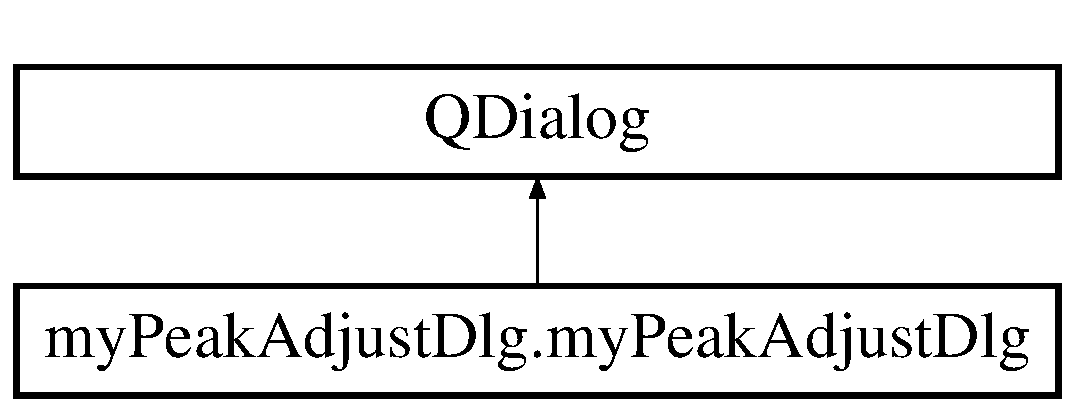
\includegraphics[height=2.000000cm]{classmyPeakAdjustDlg_1_1myPeakAdjustDlg}
\end{center}
\end{figure}
\subsection*{Public Member Functions}
\begin{DoxyCompactItemize}
\item 
\hypertarget{classmyPeakAdjustDlg_1_1myPeakAdjustDlg_abaacb5b4b52585a3c95c3709c7ddc87a}{def {\bfseries \-\_\-\-\_\-init\-\_\-\-\_\-}}\label{classmyPeakAdjustDlg_1_1myPeakAdjustDlg_abaacb5b4b52585a3c95c3709c7ddc87a}

\item 
\hypertarget{classmyPeakAdjustDlg_1_1myPeakAdjustDlg_a8a3b1f75dfe5592add8cf68686659a41}{def {\bfseries set\-Peak\-Display}}\label{classmyPeakAdjustDlg_1_1myPeakAdjustDlg_a8a3b1f75dfe5592add8cf68686659a41}

\item 
\hypertarget{classmyPeakAdjustDlg_1_1myPeakAdjustDlg_a5ff4c61e897515906ea1cf647a8ebb4e}{def {\bfseries changed\-Type}}\label{classmyPeakAdjustDlg_1_1myPeakAdjustDlg_a5ff4c61e897515906ea1cf647a8ebb4e}

\item 
\hypertarget{classmyPeakAdjustDlg_1_1myPeakAdjustDlg_ad3012bad6f6dbe3c06af6758dab86acb}{def {\bfseries update\-L\-E\-Fields}}\label{classmyPeakAdjustDlg_1_1myPeakAdjustDlg_ad3012bad6f6dbe3c06af6758dab86acb}

\item 
\hypertarget{classmyPeakAdjustDlg_1_1myPeakAdjustDlg_afde46489a42cbb16452829ef81097005}{def {\bfseries update}}\label{classmyPeakAdjustDlg_1_1myPeakAdjustDlg_afde46489a42cbb16452829ef81097005}

\end{DoxyCompactItemize}
\subsection*{Public Attributes}
\begin{DoxyCompactItemize}
\item 
\hypertarget{classmyPeakAdjustDlg_1_1myPeakAdjustDlg_a1fc76ecbe349bc391603074a7b2ca8c9}{{\bfseries ui}}\label{classmyPeakAdjustDlg_1_1myPeakAdjustDlg_a1fc76ecbe349bc391603074a7b2ca8c9}

\item 
\hypertarget{classmyPeakAdjustDlg_1_1myPeakAdjustDlg_af1e548deba0b44e985b04f37f53f4976}{{\bfseries zm\-Peak\-Fit}}\label{classmyPeakAdjustDlg_1_1myPeakAdjustDlg_af1e548deba0b44e985b04f37f53f4976}

\item 
\hypertarget{classmyPeakAdjustDlg_1_1myPeakAdjustDlg_a4c928c7791bd418243581ae926f275b6}{{\bfseries zm\-Peak\-Resids}}\label{classmyPeakAdjustDlg_1_1myPeakAdjustDlg_a4c928c7791bd418243581ae926f275b6}

\end{DoxyCompactItemize}
\subsection*{Static Public Attributes}
\begin{DoxyCompactItemize}
\item 
\hypertarget{classmyPeakAdjustDlg_1_1myPeakAdjustDlg_a9c226539269d6b35d50880d49e49dff7}{{\bfseries zm\-Peak\-Raw} = None}\label{classmyPeakAdjustDlg_1_1myPeakAdjustDlg_a9c226539269d6b35d50880d49e49dff7}

\item 
\hypertarget{classmyPeakAdjustDlg_1_1myPeakAdjustDlg_a77033ff8fcc0c925aafb76333050f5c9}{list {\bfseries raw\-Mn\-Mx} = \mbox{[}0.,0.\mbox{]}}\label{classmyPeakAdjustDlg_1_1myPeakAdjustDlg_a77033ff8fcc0c925aafb76333050f5c9}

\item 
\hypertarget{classmyPeakAdjustDlg_1_1myPeakAdjustDlg_a50b584afc0dbc9e5c7dc296325469935}{list {\bfseries fit\-Mn\-Mx} = \mbox{[}0.,0.\mbox{]}}\label{classmyPeakAdjustDlg_1_1myPeakAdjustDlg_a50b584afc0dbc9e5c7dc296325469935}

\item 
\hypertarget{classmyPeakAdjustDlg_1_1myPeakAdjustDlg_a50a4c1e4d7862bb9d67565279fc9ed6e}{list {\bfseries resids\-Mn\-Mx} = \mbox{[}0.,0.\mbox{]}}\label{classmyPeakAdjustDlg_1_1myPeakAdjustDlg_a50a4c1e4d7862bb9d67565279fc9ed6e}

\end{DoxyCompactItemize}


The documentation for this class was generated from the following file\-:\begin{DoxyCompactItemize}
\item 
/home/harold/workdir/atrex/\-Software/my\-Peak\-Adjust\-Dlg.\-py\end{DoxyCompactItemize}

\hypertarget{classmyPeaks_1_1myPeaks}{\section{my\-Peaks.\-my\-Peaks Class Reference}
\label{classmyPeaks_1_1myPeaks}\index{my\-Peaks.\-my\-Peaks@{my\-Peaks.\-my\-Peaks}}
}
Inheritance diagram for my\-Peaks.\-my\-Peaks\-:\begin{figure}[H]
\begin{center}
\leavevmode
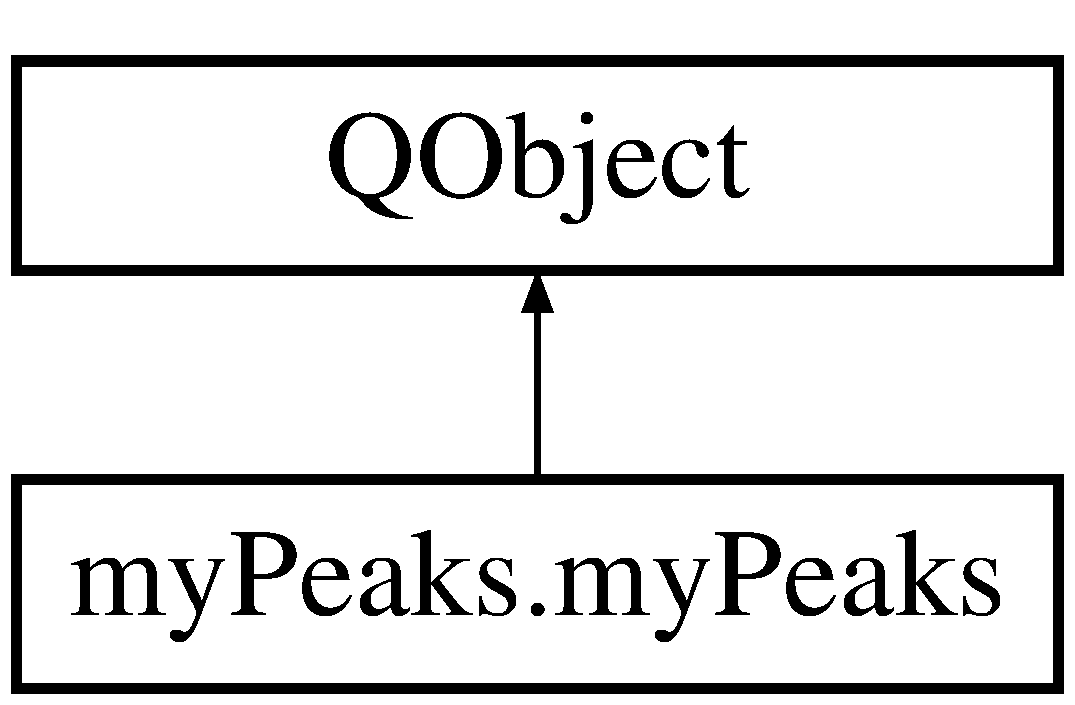
\includegraphics[height=2.000000cm]{classmyPeaks_1_1myPeaks}
\end{center}
\end{figure}
\subsection*{Public Member Functions}
\begin{DoxyCompactItemize}
\item 
\hypertarget{classmyPeaks_1_1myPeaks_a96aa94100a2cae09e55aec9b21b5c934}{def {\bfseries \-\_\-\-\_\-init\-\_\-\-\_\-}}\label{classmyPeaks_1_1myPeaks_a96aa94100a2cae09e55aec9b21b5c934}

\item 
\hypertarget{classmyPeaks_1_1myPeaks_a85b8109b49ce283142c01c4f386657f5}{def {\bfseries add\-Peak}}\label{classmyPeaks_1_1myPeaks_a85b8109b49ce283142c01c4f386657f5}

\item 
\hypertarget{classmyPeaks_1_1myPeaks_a7f167f9ae163b0025f45f3552d238b4b}{def {\bfseries set\-Active\-List}}\label{classmyPeaks_1_1myPeaks_a7f167f9ae163b0025f45f3552d238b4b}

\item 
\hypertarget{classmyPeaks_1_1myPeaks_a8a2447225e6a87f1b0273697e633ba93}{def {\bfseries set\-Selected}}\label{classmyPeaks_1_1myPeaks_a8a2447225e6a87f1b0273697e633ba93}

\item 
\hypertarget{classmyPeaks_1_1myPeaks_ab4288640f1dd2ea00b5aaa48d11014c4}{def {\bfseries select\-All}}\label{classmyPeaks_1_1myPeaks_ab4288640f1dd2ea00b5aaa48d11014c4}

\item 
\hypertarget{classmyPeaks_1_1myPeaks_aecd844074c5479e3379981ad71b85981}{def {\bfseries clear\-All}}\label{classmyPeaks_1_1myPeaks_aecd844074c5479e3379981ad71b85981}

\item 
\hypertarget{classmyPeaks_1_1myPeaks_a0da9e1901691583a56fb3784eedc91f7}{def {\bfseries delete\-Selected}}\label{classmyPeaks_1_1myPeaks_a0da9e1901691583a56fb3784eedc91f7}

\item 
\hypertarget{classmyPeaks_1_1myPeaks_a90a5f3241c94520978668e1a3f62774e}{def {\bfseries move\-Selected}}\label{classmyPeaks_1_1myPeaks_a90a5f3241c94520978668e1a3f62774e}

\end{DoxyCompactItemize}
\subsection*{Public Attributes}
\begin{DoxyCompactItemize}
\item 
\hypertarget{classmyPeaks_1_1myPeaks_ab764afe03c88786678b9b63fa09337ef}{{\bfseries active\-List}}\label{classmyPeaks_1_1myPeaks_ab764afe03c88786678b9b63fa09337ef}

\end{DoxyCompactItemize}
\subsection*{Static Public Attributes}
\begin{DoxyCompactItemize}
\item 
\hypertarget{classmyPeaks_1_1myPeaks_a188582bdcbbda828a9d44fd7336570d8}{list {\bfseries peaks\-\_\-0} = \mbox{[}$\,$\mbox{]}}\label{classmyPeaks_1_1myPeaks_a188582bdcbbda828a9d44fd7336570d8}

\item 
\hypertarget{classmyPeaks_1_1myPeaks_acba3b1f63dcd097b793f8cbcb0e0befc}{list {\bfseries peaks\-\_\-1} = \mbox{[}$\,$\mbox{]}}\label{classmyPeaks_1_1myPeaks_acba3b1f63dcd097b793f8cbcb0e0befc}

\item 
\hypertarget{classmyPeaks_1_1myPeaks_a769d8400c803069ed2de73079e5e8b08}{list {\bfseries peak\-Lists} = \mbox{[}peaks\-\_\-0,peaks\-\_\-1\mbox{]}}\label{classmyPeaks_1_1myPeaks_a769d8400c803069ed2de73079e5e8b08}

\item 
\hypertarget{classmyPeaks_1_1myPeaks_ae28250cdc31d2022b52ebd0b35b61ad9}{int {\bfseries active\-List} = 0}\label{classmyPeaks_1_1myPeaks_ae28250cdc31d2022b52ebd0b35b61ad9}

\end{DoxyCompactItemize}


The documentation for this class was generated from the following file\-:\begin{DoxyCompactItemize}
\item 
/home/harold/workdir/atrex/\-Software/my\-Peaks.\-py\end{DoxyCompactItemize}

\hypertarget{classmyPeakTable_1_1myPeakTable}{\section{my\-Peak\-Table.\-my\-Peak\-Table Class Reference}
\label{classmyPeakTable_1_1myPeakTable}\index{my\-Peak\-Table.\-my\-Peak\-Table@{my\-Peak\-Table.\-my\-Peak\-Table}}
}
\subsection*{Public Member Functions}
\begin{DoxyCompactItemize}
\item 
\hypertarget{classmyPeakTable_1_1myPeakTable_af91b0ff7c386b74e34eaadf5228fc89c}{def {\bfseries \-\_\-\-\_\-init\-\_\-\-\_\-}}\label{classmyPeakTable_1_1myPeakTable_af91b0ff7c386b74e34eaadf5228fc89c}

\item 
\hypertarget{classmyPeakTable_1_1myPeakTable_ae353c401abe1c75d8cffeb5277615d70}{def {\bfseries zero}}\label{classmyPeakTable_1_1myPeakTable_ae353c401abe1c75d8cffeb5277615d70}

\item 
\hypertarget{classmyPeakTable_1_1myPeakTable_a8171aa9d50a86f7483d840ad094f77c5}{def {\bfseries set\-Selected}}\label{classmyPeakTable_1_1myPeakTable_a8171aa9d50a86f7483d840ad094f77c5}

\item 
\hypertarget{classmyPeakTable_1_1myPeakTable_aa543910f172ce15483e4753d848a296e}{def {\bfseries set\-Unselected}}\label{classmyPeakTable_1_1myPeakTable_aa543910f172ce15483e4753d848a296e}

\item 
\hypertarget{classmyPeakTable_1_1myPeakTable_aecda5256aaa268233ca76fc9aa31ea57}{def {\bfseries get\-Peaklist\-Det\-X}}\label{classmyPeakTable_1_1myPeakTable_aecda5256aaa268233ca76fc9aa31ea57}

\item 
\hypertarget{classmyPeakTable_1_1myPeakTable_ae754776fe2219a19ea8421154ec97c83}{def {\bfseries get\-Peaklist\-Det\-Y}}\label{classmyPeakTable_1_1myPeakTable_ae754776fe2219a19ea8421154ec97c83}

\item 
\hypertarget{classmyPeakTable_1_1myPeakTable_ab5033bca2519e7d553ff31abffe31b45}{def {\bfseries copy\-\_\-peaktable}}\label{classmyPeakTable_1_1myPeakTable_ab5033bca2519e7d553ff31abffe31b45}

\item 
\hypertarget{classmyPeakTable_1_1myPeakTable_a2632e23b330621bc8c0db28f103b6f4b}{def {\bfseries set\-Active\-List}}\label{classmyPeakTable_1_1myPeakTable_a2632e23b330621bc8c0db28f103b6f4b}

\item 
\hypertarget{classmyPeakTable_1_1myPeakTable_aeae41fc2195c4a8e762733b10bb16037}{def {\bfseries delete\-Selected}}\label{classmyPeakTable_1_1myPeakTable_aeae41fc2195c4a8e762733b10bb16037}

\item 
\hypertarget{classmyPeakTable_1_1myPeakTable_af0e5527f60c61c6c71c5a06740ccbb1a}{def {\bfseries move\-Selected}}\label{classmyPeakTable_1_1myPeakTable_af0e5527f60c61c6c71c5a06740ccbb1a}

\item 
\hypertarget{classmyPeakTable_1_1myPeakTable_afd55f45ebb0ff7a220abfc077476ab7e}{def {\bfseries getpeakno}}\label{classmyPeakTable_1_1myPeakTable_afd55f45ebb0ff7a220abfc077476ab7e}

\item 
\hypertarget{classmyPeakTable_1_1myPeakTable_ac4307c79c6fbe7939ba91c8b8e863e1e}{def {\bfseries get\-\_\-peaks}}\label{classmyPeakTable_1_1myPeakTable_ac4307c79c6fbe7939ba91c8b8e863e1e}

\item 
\hypertarget{classmyPeakTable_1_1myPeakTable_a44cf0204f3e6c72e1e38110aa1c17812}{def {\bfseries getonepeak}}\label{classmyPeakTable_1_1myPeakTable_a44cf0204f3e6c72e1e38110aa1c17812}

\item 
\hypertarget{classmyPeakTable_1_1myPeakTable_a8d97309248cdbbd80bb15151d57f2d19}{def {\bfseries getselectedno}}\label{classmyPeakTable_1_1myPeakTable_a8d97309248cdbbd80bb15151d57f2d19}

\item 
\hypertarget{classmyPeakTable_1_1myPeakTable_a5597961217d00620e9528fc283cdaa34}{def {\bfseries setpeakno}}\label{classmyPeakTable_1_1myPeakTable_a5597961217d00620e9528fc283cdaa34}

\item 
\hypertarget{classmyPeakTable_1_1myPeakTable_a145f32c055bd6f844f0dc2eea559c7a1}{def {\bfseries add\-Peak}}\label{classmyPeakTable_1_1myPeakTable_a145f32c055bd6f844f0dc2eea559c7a1}

\item 
\hypertarget{classmyPeakTable_1_1myPeakTable_af672cd80fa6edc133258f8d02a6066cd}{def {\bfseries remove\-Peaks}}\label{classmyPeakTable_1_1myPeakTable_af672cd80fa6edc133258f8d02a6066cd}

\item 
\hypertarget{classmyPeakTable_1_1myPeakTable_abec9c6e424ad7d7fdd4d222dd48f4059}{def {\bfseries select\-Peaks}}\label{classmyPeakTable_1_1myPeakTable_abec9c6e424ad7d7fdd4d222dd48f4059}

\item 
\hypertarget{classmyPeakTable_1_1myPeakTable_ad1242828b8b1857958f477e816e53e50}{def {\bfseries unselect\-Peak}}\label{classmyPeakTable_1_1myPeakTable_ad1242828b8b1857958f477e816e53e50}

\item 
\hypertarget{classmyPeakTable_1_1myPeakTable_a45c06af5936ee97b75fcb2f51c6f2809}{def {\bfseries unselect\-All}}\label{classmyPeakTable_1_1myPeakTable_a45c06af5936ee97b75fcb2f51c6f2809}

\item 
\hypertarget{classmyPeakTable_1_1myPeakTable_a7f0337470250c257cd8b5492bb407a34}{def {\bfseries select\-All}}\label{classmyPeakTable_1_1myPeakTable_a7f0337470250c257cd8b5492bb407a34}

\item 
\hypertarget{classmyPeakTable_1_1myPeakTable_a9067cdbb5a19a158bcb515417be4c5d2}{def {\bfseries write\-\_\-to\-\_\-file}}\label{classmyPeakTable_1_1myPeakTable_a9067cdbb5a19a158bcb515417be4c5d2}

\item 
\hypertarget{classmyPeakTable_1_1myPeakTable_af5422088cd0a8443c5275ee1f7a598b3}{def {\bfseries write\-\_\-to\-\_\-file\-A}}\label{classmyPeakTable_1_1myPeakTable_af5422088cd0a8443c5275ee1f7a598b3}

\item 
\hypertarget{classmyPeakTable_1_1myPeakTable_abac87e56abbdbf3cd26fe1e45b5ba4b4}{def {\bfseries read\-\_\-from\-\_\-file\-A}}\label{classmyPeakTable_1_1myPeakTable_abac87e56abbdbf3cd26fe1e45b5ba4b4}

\item 
\hypertarget{classmyPeakTable_1_1myPeakTable_accfb27ea1b0363b5bb88fcd0e9c211c6}{def {\bfseries read\-\_\-from\-\_\-file}}\label{classmyPeakTable_1_1myPeakTable_accfb27ea1b0363b5bb88fcd0e9c211c6}

\item 
\hypertarget{classmyPeakTable_1_1myPeakTable_a27f05c63eb11d1ebc986d84b3ce82144}{def {\bfseries truncate}}\label{classmyPeakTable_1_1myPeakTable_a27f05c63eb11d1ebc986d84b3ce82144}

\item 
\hypertarget{classmyPeakTable_1_1myPeakTable_ac19edb546ca91e7fce0bbb167ed19876}{def {\bfseries remove\-\_\-all\-\_\-peaks}}\label{classmyPeakTable_1_1myPeakTable_ac19edb546ca91e7fce0bbb167ed19876}

\item 
\hypertarget{classmyPeakTable_1_1myPeakTable_af76096f9d9b0722727defc71f5465450}{def {\bfseries calculate\-\_\-all\-\_\-xyz\-\_\-from\-\_\-pix}}\label{classmyPeakTable_1_1myPeakTable_af76096f9d9b0722727defc71f5465450}

\item 
\hypertarget{classmyPeakTable_1_1myPeakTable_a048b6f02a598f8528b9e4a7a48c66d80}{def {\bfseries remove\-\_\-peaks\-\_\-outside\-\_\-aa}}\label{classmyPeakTable_1_1myPeakTable_a048b6f02a598f8528b9e4a7a48c66d80}

\item 
\hypertarget{classmyPeakTable_1_1myPeakTable_a4c84d1c677df5d806a0fe898171f32dd}{def {\bfseries find\-\_\-closest\-\_\-peak}}\label{classmyPeakTable_1_1myPeakTable_a4c84d1c677df5d806a0fe898171f32dd}

\item 
\hypertarget{classmyPeakTable_1_1myPeakTable_a1500b118c12ebc5d8cd9c4ac392a7037}{def {\bfseries find\-\_\-close\-\_\-overlaps}}\label{classmyPeakTable_1_1myPeakTable_a1500b118c12ebc5d8cd9c4ac392a7037}

\item 
\hypertarget{classmyPeakTable_1_1myPeakTable_af90e10c7f0a6286b59b47a801d630241}{def {\bfseries find\-\_\-multiple\-\_\-peak\-\_\-copies}}\label{classmyPeakTable_1_1myPeakTable_af90e10c7f0a6286b59b47a801d630241}

\item 
\hypertarget{classmyPeakTable_1_1myPeakTable_a0ecc469a4774f19b94bd986fe4033009}{def {\bfseries select\-\_\-close\-\_\-overlaps}}\label{classmyPeakTable_1_1myPeakTable_a0ecc469a4774f19b94bd986fe4033009}

\item 
\hypertarget{classmyPeakTable_1_1myPeakTable_acd681ebee5454e3b2d99fdd0ddfdbd11}{def {\bfseries get\-Dist}}\label{classmyPeakTable_1_1myPeakTable_acd681ebee5454e3b2d99fdd0ddfdbd11}

\item 
\hypertarget{classmyPeakTable_1_1myPeakTable_a5e43b3eca47216d977185cff9abb46d1}{def {\bfseries save\-\_\-p4p}}\label{classmyPeakTable_1_1myPeakTable_a5e43b3eca47216d977185cff9abb46d1}

\end{DoxyCompactItemize}
\subsection*{Public Attributes}
\begin{DoxyCompactItemize}
\item 
\hypertarget{classmyPeakTable_1_1myPeakTable_ac5e5fdd422bfd17223d9424c75ac5e57}{{\bfseries peakno}}\label{classmyPeakTable_1_1myPeakTable_ac5e5fdd422bfd17223d9424c75ac5e57}

\item 
\hypertarget{classmyPeakTable_1_1myPeakTable_aa7213ccc67f2d998076ef95396d53d01}{{\bfseries selectedno}}\label{classmyPeakTable_1_1myPeakTable_aa7213ccc67f2d998076ef95396d53d01}

\item 
\hypertarget{classmyPeakTable_1_1myPeakTable_a4e6db53861997b42cc4886dca5593b4d}{{\bfseries peaks}}\label{classmyPeakTable_1_1myPeakTable_a4e6db53861997b42cc4886dca5593b4d}

\item 
\hypertarget{classmyPeakTable_1_1myPeakTable_a59227cea4995b2a3a5b7423ccb0d712c}{{\bfseries active\-List}}\label{classmyPeakTable_1_1myPeakTable_a59227cea4995b2a3a5b7423ccb0d712c}

\item 
\hypertarget{classmyPeakTable_1_1myPeakTable_ac746b90e0b88d62891770a0c82a6366c}{{\bfseries peaks1}}\label{classmyPeakTable_1_1myPeakTable_ac746b90e0b88d62891770a0c82a6366c}

\item 
\hypertarget{classmyPeakTable_1_1myPeakTable_af40587b94cba8e86cd5e790a2f6eb062}{{\bfseries peaks0}}\label{classmyPeakTable_1_1myPeakTable_af40587b94cba8e86cd5e790a2f6eb062}

\end{DoxyCompactItemize}


The documentation for this class was generated from the following file\-:\begin{DoxyCompactItemize}
\item 
/home/harold/workdir/atrex/\-Software/my\-Peak\-Table.\-py\end{DoxyCompactItemize}

\hypertarget{classmyPeakTableWidget_1_1myPeakTableWidget}{\section{my\-Peak\-Table\-Widget.\-my\-Peak\-Table\-Widget Class Reference}
\label{classmyPeakTableWidget_1_1myPeakTableWidget}\index{my\-Peak\-Table\-Widget.\-my\-Peak\-Table\-Widget@{my\-Peak\-Table\-Widget.\-my\-Peak\-Table\-Widget}}
}
Inheritance diagram for my\-Peak\-Table\-Widget.\-my\-Peak\-Table\-Widget\-:\begin{figure}[H]
\begin{center}
\leavevmode
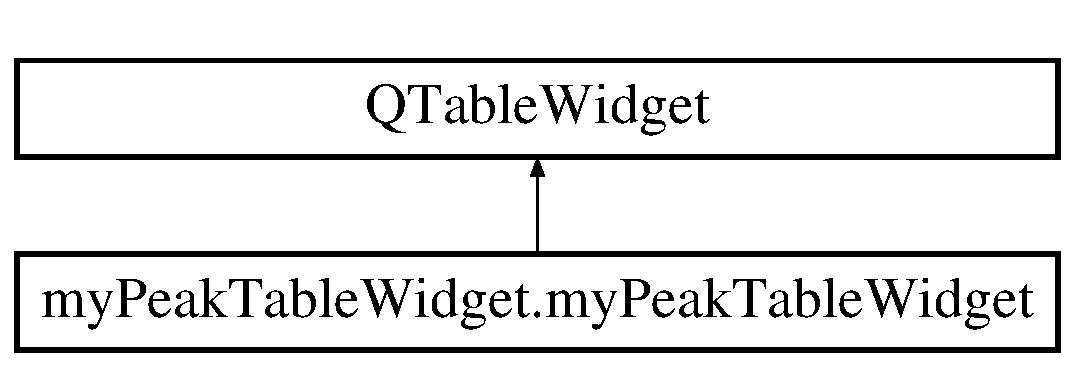
\includegraphics[height=2.000000cm]{classmyPeakTableWidget_1_1myPeakTableWidget}
\end{center}
\end{figure}
\subsection*{Public Member Functions}
\begin{DoxyCompactItemize}
\item 
\hypertarget{classmyPeakTableWidget_1_1myPeakTableWidget_a112e9c9fe94f89bee7313906355d6c8f}{def {\bfseries \-\_\-\-\_\-init\-\_\-\-\_\-}}\label{classmyPeakTableWidget_1_1myPeakTableWidget_a112e9c9fe94f89bee7313906355d6c8f}

\item 
\hypertarget{classmyPeakTableWidget_1_1myPeakTableWidget_abc9980e6816ae93b1302da488b1eb83b}{def {\bfseries set\-Image\-File\-Name}}\label{classmyPeakTableWidget_1_1myPeakTableWidget_abc9980e6816ae93b1302da488b1eb83b}

\item 
\hypertarget{classmyPeakTableWidget_1_1myPeakTableWidget_a30d9b900b3a8eb5fac45aacdd1355b4c}{def {\bfseries set\-Detector}}\label{classmyPeakTableWidget_1_1myPeakTableWidget_a30d9b900b3a8eb5fac45aacdd1355b4c}

\item 
\hypertarget{classmyPeakTableWidget_1_1myPeakTableWidget_a3c7bc1e38db2eb6e0458a438a753f6c3}{def {\bfseries set\-Peaks}}\label{classmyPeakTableWidget_1_1myPeakTableWidget_a3c7bc1e38db2eb6e0458a438a753f6c3}

\item 
\hypertarget{classmyPeakTableWidget_1_1myPeakTableWidget_aa4aed89efa31348e87d73f711d996daf}{def {\bfseries add\-Peak}}\label{classmyPeakTableWidget_1_1myPeakTableWidget_aa4aed89efa31348e87d73f711d996daf}

\item 
\hypertarget{classmyPeakTableWidget_1_1myPeakTableWidget_ac06c362f6d4a47181fbcc0fe2e78a2cb}{def {\bfseries peak\-Edit}}\label{classmyPeakTableWidget_1_1myPeakTableWidget_ac06c362f6d4a47181fbcc0fe2e78a2cb}

\end{DoxyCompactItemize}
\subsection*{Public Attributes}
\begin{DoxyCompactItemize}
\item 
\hypertarget{classmyPeakTableWidget_1_1myPeakTableWidget_ac482a5f93ba7061a3a6e8c6d46e2e26b}{{\bfseries imfile}}\label{classmyPeakTableWidget_1_1myPeakTableWidget_ac482a5f93ba7061a3a6e8c6d46e2e26b}

\item 
\hypertarget{classmyPeakTableWidget_1_1myPeakTableWidget_a9c8259e29d4d739d45452eaec8bebff0}{{\bfseries my\-Det}}\label{classmyPeakTableWidget_1_1myPeakTableWidget_a9c8259e29d4d739d45452eaec8bebff0}

\item 
\hypertarget{classmyPeakTableWidget_1_1myPeakTableWidget_afa4b43bf4a5bf3308bf8a7d4c146712b}{{\bfseries peaks}}\label{classmyPeakTableWidget_1_1myPeakTableWidget_afa4b43bf4a5bf3308bf8a7d4c146712b}

\item 
\hypertarget{classmyPeakTableWidget_1_1myPeakTableWidget_ae4934e86392397c16937ababde3ac38e}{{\bfseries num\-Peaks}}\label{classmyPeakTableWidget_1_1myPeakTableWidget_ae4934e86392397c16937ababde3ac38e}

\end{DoxyCompactItemize}
\subsection*{Static Public Attributes}
\begin{DoxyCompactItemize}
\item 
\hypertarget{classmyPeakTableWidget_1_1myPeakTableWidget_a8e630a6f15d224300abc621b8bac8e23}{int {\bfseries num\-Peaks} = 0}\label{classmyPeakTableWidget_1_1myPeakTableWidget_a8e630a6f15d224300abc621b8bac8e23}

\item 
\hypertarget{classmyPeakTableWidget_1_1myPeakTableWidget_a6b0c16aabbedcc000d20542e5d4b3e08}{tuple {\bfseries head\-List} = Qt\-Core.\-Q\-String(\char`\"{}X;Y;2-\/theta;d-\/spacing;h;k;l;rot. angle\char`\"{})}\label{classmyPeakTableWidget_1_1myPeakTableWidget_a6b0c16aabbedcc000d20542e5d4b3e08}

\item 
\hypertarget{classmyPeakTableWidget_1_1myPeakTableWidget_a7be636c918a7d4e642015b4531795477}{int {\bfseries my\-Det} = 0}\label{classmyPeakTableWidget_1_1myPeakTableWidget_a7be636c918a7d4e642015b4531795477}

\item 
\hypertarget{classmyPeakTableWidget_1_1myPeakTableWidget_a00a3801ee16f8bb1b140b254793e098c}{int {\bfseries peaks} = 0}\label{classmyPeakTableWidget_1_1myPeakTableWidget_a00a3801ee16f8bb1b140b254793e098c}

\item 
\hypertarget{classmyPeakTableWidget_1_1myPeakTableWidget_ae072cce7f45a7c9a7c4a4d6ea9887593}{string {\bfseries imname} = ''}\label{classmyPeakTableWidget_1_1myPeakTableWidget_ae072cce7f45a7c9a7c4a4d6ea9887593}

\end{DoxyCompactItemize}


The documentation for this class was generated from the following file\-:\begin{DoxyCompactItemize}
\item 
/home/harold/workdir/atrex/\-Software/my\-Peak\-Table\-Widget.\-py\end{DoxyCompactItemize}

\hypertarget{classMyPlotWidget_1_1MyPlotWidget}{\section{My\-Plot\-Widget.\-My\-Plot\-Widget Class Reference}
\label{classMyPlotWidget_1_1MyPlotWidget}\index{My\-Plot\-Widget.\-My\-Plot\-Widget@{My\-Plot\-Widget.\-My\-Plot\-Widget}}
}
Inheritance diagram for My\-Plot\-Widget.\-My\-Plot\-Widget\-:\begin{figure}[H]
\begin{center}
\leavevmode
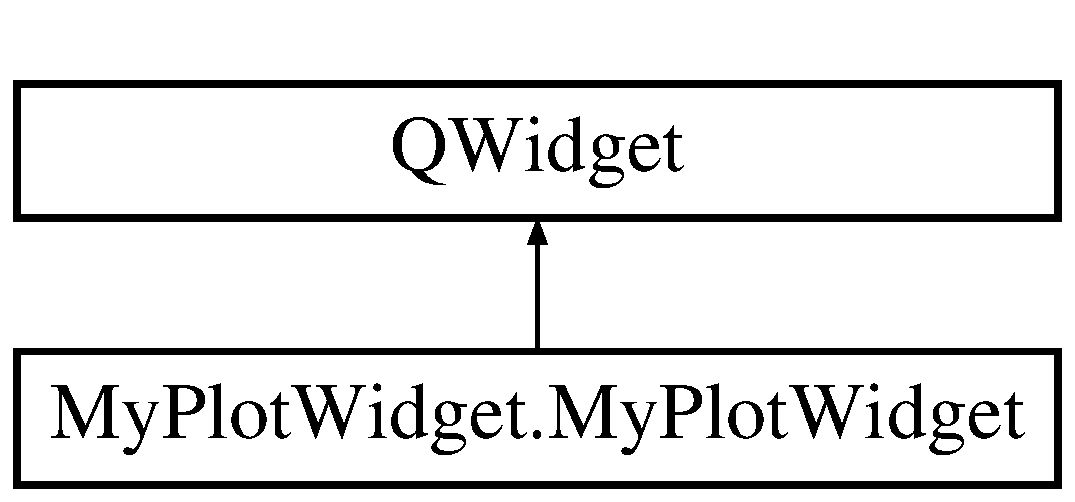
\includegraphics[height=2.000000cm]{classMyPlotWidget_1_1MyPlotWidget}
\end{center}
\end{figure}
\subsection*{Public Member Functions}
\begin{DoxyCompactItemize}
\item 
\hypertarget{classMyPlotWidget_1_1MyPlotWidget_a6609ab444ac92ada3d856756c4d63ff3}{def {\bfseries \-\_\-\-\_\-init\-\_\-\-\_\-}}\label{classMyPlotWidget_1_1MyPlotWidget_a6609ab444ac92ada3d856756c4d63ff3}

\item 
\hypertarget{classMyPlotWidget_1_1MyPlotWidget_a7cc35e9fdcea629d444e69c9be1f17e5}{def {\bfseries size\-Hint}}\label{classMyPlotWidget_1_1MyPlotWidget_a7cc35e9fdcea629d444e69c9be1f17e5}

\item 
\hypertarget{classMyPlotWidget_1_1MyPlotWidget_a24bbe5fb4b29afdb328e65616fd49607}{def {\bfseries minimum\-Size\-Hint}}\label{classMyPlotWidget_1_1MyPlotWidget_a24bbe5fb4b29afdb328e65616fd49607}

\item 
\hypertarget{classMyPlotWidget_1_1MyPlotWidget_a51f5c70ea2dd4024e4c56a0a73925164}{def {\bfseries plot\-Data}}\label{classMyPlotWidget_1_1MyPlotWidget_a51f5c70ea2dd4024e4c56a0a73925164}

\item 
\hypertarget{classMyPlotWidget_1_1MyPlotWidget_aa715ad5a13d60bef1d1d8f35d17a128d}{def {\bfseries plot\-Data\-X\-Y2}}\label{classMyPlotWidget_1_1MyPlotWidget_aa715ad5a13d60bef1d1d8f35d17a128d}

\item 
\hypertarget{classMyPlotWidget_1_1MyPlotWidget_adf3455693401acc7a41cc2b167c8ea7d}{def {\bfseries set\-X\-Y\-Data}}\label{classMyPlotWidget_1_1MyPlotWidget_adf3455693401acc7a41cc2b167c8ea7d}

\item 
\hypertarget{classMyPlotWidget_1_1MyPlotWidget_a6298a336d89650749a4c04e28bcf4274}{def {\bfseries set\-Overlay\-X\-Y\-Data}}\label{classMyPlotWidget_1_1MyPlotWidget_a6298a336d89650749a4c04e28bcf4274}

\item 
\hypertarget{classMyPlotWidget_1_1MyPlotWidget_ac55f01d08b5bf74fe1bfeb2719747a92}{def {\bfseries set\-X\-Y\-Data\-\_\-\-Integrate}}\label{classMyPlotWidget_1_1MyPlotWidget_ac55f01d08b5bf74fe1bfeb2719747a92}

\item 
\hypertarget{classMyPlotWidget_1_1MyPlotWidget_a2ba64fd7e8dd68a755267f4fbcde2b45}{def {\bfseries create\-Cos\-Data}}\label{classMyPlotWidget_1_1MyPlotWidget_a2ba64fd7e8dd68a755267f4fbcde2b45}

\item 
\hypertarget{classMyPlotWidget_1_1MyPlotWidget_a866f749621b291e90310593be2c612f8}{def {\bfseries setp\-Type}}\label{classMyPlotWidget_1_1MyPlotWidget_a866f749621b291e90310593be2c612f8}

\item 
\hypertarget{classMyPlotWidget_1_1MyPlotWidget_a9363485b431a40f93626e21842248589}{def {\bfseries set\-Labels}}\label{classMyPlotWidget_1_1MyPlotWidget_a9363485b431a40f93626e21842248589}

\item 
\hypertarget{classMyPlotWidget_1_1MyPlotWidget_ae782a56a3f86e3e4a7c57fcc3ab55fa7}{def {\bfseries output\-To\-File}}\label{classMyPlotWidget_1_1MyPlotWidget_ae782a56a3f86e3e4a7c57fcc3ab55fa7}

\end{DoxyCompactItemize}
\subsection*{Public Attributes}
\begin{DoxyCompactItemize}
\item 
\hypertarget{classMyPlotWidget_1_1MyPlotWidget_a3f90de6f5ac0f2f681457c7d1db66422}{{\bfseries figure}}\label{classMyPlotWidget_1_1MyPlotWidget_a3f90de6f5ac0f2f681457c7d1db66422}

\item 
\hypertarget{classMyPlotWidget_1_1MyPlotWidget_ae40a5f04a117f5863db217e6134cde3a}{{\bfseries canvas}}\label{classMyPlotWidget_1_1MyPlotWidget_ae40a5f04a117f5863db217e6134cde3a}

\item 
\hypertarget{classMyPlotWidget_1_1MyPlotWidget_a5c0d1b439e1708a9e105e9c1123ba19c}{{\bfseries toolbar}}\label{classMyPlotWidget_1_1MyPlotWidget_a5c0d1b439e1708a9e105e9c1123ba19c}

\item 
\hypertarget{classMyPlotWidget_1_1MyPlotWidget_afdd3a63e478b90f8a9d43d813eef44f3}{{\bfseries axes}}\label{classMyPlotWidget_1_1MyPlotWidget_afdd3a63e478b90f8a9d43d813eef44f3}

\item 
\hypertarget{classMyPlotWidget_1_1MyPlotWidget_a4a63c84c067d764fcdef1e84b36331a4}{{\bfseries p\-Type}}\label{classMyPlotWidget_1_1MyPlotWidget_a4a63c84c067d764fcdef1e84b36331a4}

\item 
\hypertarget{classMyPlotWidget_1_1MyPlotWidget_a1ca45f1c4b0bea8328ca2926126f0468}{{\bfseries tstr}}\label{classMyPlotWidget_1_1MyPlotWidget_a1ca45f1c4b0bea8328ca2926126f0468}

\item 
\hypertarget{classMyPlotWidget_1_1MyPlotWidget_a07aaae96f1d5667f6125cf6bf7274a14}{{\bfseries xstr}}\label{classMyPlotWidget_1_1MyPlotWidget_a07aaae96f1d5667f6125cf6bf7274a14}

\item 
\hypertarget{classMyPlotWidget_1_1MyPlotWidget_a1257bc7678d216ec50d9cafa6329c8a7}{{\bfseries ystr}}\label{classMyPlotWidget_1_1MyPlotWidget_a1257bc7678d216ec50d9cafa6329c8a7}

\item 
\hypertarget{classMyPlotWidget_1_1MyPlotWidget_aa95c6b8ff2b9952b5f4fdca6b5aa2901}{{\bfseries olay\-Flag}}\label{classMyPlotWidget_1_1MyPlotWidget_aa95c6b8ff2b9952b5f4fdca6b5aa2901}

\item 
\hypertarget{classMyPlotWidget_1_1MyPlotWidget_a64e693fbacbde23a8c8d08899aa6dcdd}{{\bfseries plot\-Data\-Flag}}\label{classMyPlotWidget_1_1MyPlotWidget_a64e693fbacbde23a8c8d08899aa6dcdd}

\item 
\hypertarget{classMyPlotWidget_1_1MyPlotWidget_af8e35141d9588e42805da0c06bcffd32}{{\bfseries xarr}}\label{classMyPlotWidget_1_1MyPlotWidget_af8e35141d9588e42805da0c06bcffd32}

\item 
\hypertarget{classMyPlotWidget_1_1MyPlotWidget_aa1b1b70359cb0139710db0982040778b}{{\bfseries yarr}}\label{classMyPlotWidget_1_1MyPlotWidget_aa1b1b70359cb0139710db0982040778b}

\item 
\hypertarget{classMyPlotWidget_1_1MyPlotWidget_ada9f240a51b2615a25fef530c4028350}{{\bfseries x10}}\label{classMyPlotWidget_1_1MyPlotWidget_ada9f240a51b2615a25fef530c4028350}

\item 
\hypertarget{classMyPlotWidget_1_1MyPlotWidget_a2bcd4bfd7b9d5c75e58140845b87508d}{{\bfseries yarr\-Spline}}\label{classMyPlotWidget_1_1MyPlotWidget_a2bcd4bfd7b9d5c75e58140845b87508d}

\item 
\hypertarget{classMyPlotWidget_1_1MyPlotWidget_ad4ac85f27d3aded8658bb61a50c3f72e}{{\bfseries xarr\-Olay}}\label{classMyPlotWidget_1_1MyPlotWidget_ad4ac85f27d3aded8658bb61a50c3f72e}

\item 
\hypertarget{classMyPlotWidget_1_1MyPlotWidget_a26308ed5767dd716db3984aa549fddef}{{\bfseries yarr\-Olay}}\label{classMyPlotWidget_1_1MyPlotWidget_a26308ed5767dd716db3984aa549fddef}

\end{DoxyCompactItemize}


The documentation for this class was generated from the following file\-:\begin{DoxyCompactItemize}
\item 
/home/harold/workdir/atrex/\-Software/My\-Plot\-Widget.\-py\end{DoxyCompactItemize}

\hypertarget{classmyPredict_1_1myPredict}{\section{my\-Predict.\-my\-Predict Class Reference}
\label{classmyPredict_1_1myPredict}\index{my\-Predict.\-my\-Predict@{my\-Predict.\-my\-Predict}}
}
\subsection*{Static Public Attributes}
\begin{DoxyCompactItemize}
\item 
\hypertarget{classmyPredict_1_1myPredict_a22120f9618f06acd8650c15c08825c80}{int {\bfseries om\-\_\-start} = 0}\label{classmyPredict_1_1myPredict_a22120f9618f06acd8650c15c08825c80}

\item 
\hypertarget{classmyPredict_1_1myPredict_a4b21c39ba945630d9b575427e578ca96}{int {\bfseries om\-\_\-range} = 0}\label{classmyPredict_1_1myPredict_a4b21c39ba945630d9b575427e578ca96}

\item 
\hypertarget{classmyPredict_1_1myPredict_a628dfab0d8a8cd900af38f69d58ea96a}{int {\bfseries chi} = 0}\label{classmyPredict_1_1myPredict_a628dfab0d8a8cd900af38f69d58ea96a}

\item 
\hypertarget{classmyPredict_1_1myPredict_ad000055f5486abf5e3ad766e1170775f}{int {\bfseries d} = 0}\label{classmyPredict_1_1myPredict_ad000055f5486abf5e3ad766e1170775f}

\item 
\hypertarget{classmyPredict_1_1myPredict_abf3a46e4bd94b6d14263dacd22c9cb24}{int {\bfseries h1} = -\/25}\label{classmyPredict_1_1myPredict_abf3a46e4bd94b6d14263dacd22c9cb24}

\item 
\hypertarget{classmyPredict_1_1myPredict_a1193984f0a6fde8ddbca73c1c027294a}{int {\bfseries h2} = 25}\label{classmyPredict_1_1myPredict_a1193984f0a6fde8ddbca73c1c027294a}

\item 
\hypertarget{classmyPredict_1_1myPredict_a36f7425581e5d92e7ae40a14c731cc9c}{int {\bfseries k1} = -\/25}\label{classmyPredict_1_1myPredict_a36f7425581e5d92e7ae40a14c731cc9c}

\item 
\hypertarget{classmyPredict_1_1myPredict_a25decbee9aa99c6106854776fdeca4bb}{int {\bfseries k2} = 25}\label{classmyPredict_1_1myPredict_a25decbee9aa99c6106854776fdeca4bb}

\item 
\hypertarget{classmyPredict_1_1myPredict_a6b9c00f63edbf64fb570418b1f1a6905}{int {\bfseries l1} = -\/25}\label{classmyPredict_1_1myPredict_a6b9c00f63edbf64fb570418b1f1a6905}

\item 
\hypertarget{classmyPredict_1_1myPredict_a0bc5d7a9a57b15ae0c59e43e8e83d56e}{int {\bfseries l2} = 25}\label{classmyPredict_1_1myPredict_a0bc5d7a9a57b15ae0c59e43e8e83d56e}

\item 
\hypertarget{classmyPredict_1_1myPredict_a984cd2295737fe88f8e0d5e34070bf67}{int {\bfseries dac\-\_\-open} = 18}\label{classmyPredict_1_1myPredict_a984cd2295737fe88f8e0d5e34070bf67}

\end{DoxyCompactItemize}


The documentation for this class was generated from the following file\-:\begin{DoxyCompactItemize}
\item 
/home/harold/workdir/atrex/\-Software/my\-Predict.\-py\end{DoxyCompactItemize}

\hypertarget{classmyZmDisplay_1_1myZmDisplay}{\section{my\-Zm\-Display.\-my\-Zm\-Display Class Reference}
\label{classmyZmDisplay_1_1myZmDisplay}\index{my\-Zm\-Display.\-my\-Zm\-Display@{my\-Zm\-Display.\-my\-Zm\-Display}}
}
Inheritance diagram for my\-Zm\-Display.\-my\-Zm\-Display\-:\begin{figure}[H]
\begin{center}
\leavevmode
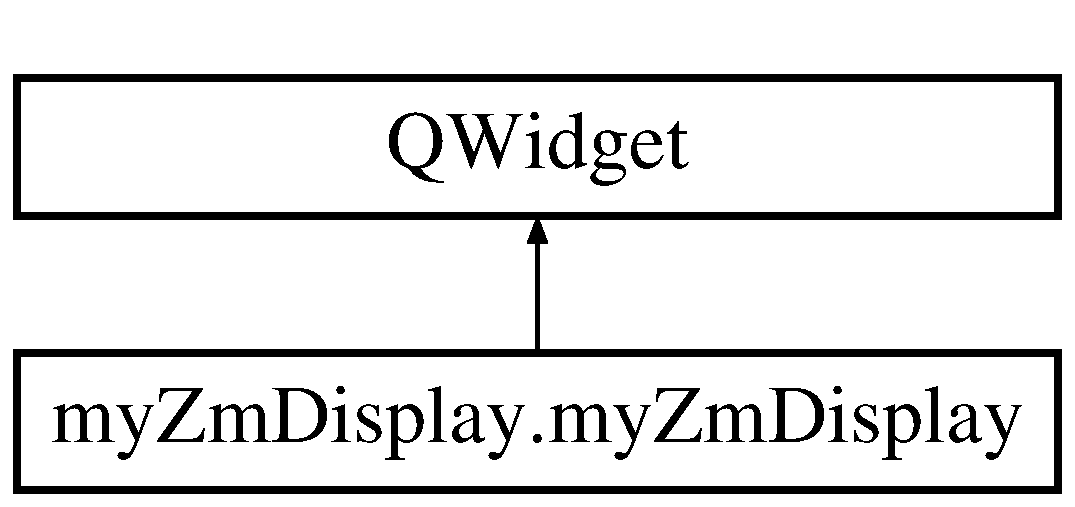
\includegraphics[height=2.000000cm]{classmyZmDisplay_1_1myZmDisplay}
\end{center}
\end{figure}
\subsection*{Public Member Functions}
\begin{DoxyCompactItemize}
\item 
\hypertarget{classmyZmDisplay_1_1myZmDisplay_a54641fdc112a59527b6d8f449f7d37c7}{def {\bfseries \-\_\-\-\_\-init\-\_\-\-\_\-}}\label{classmyZmDisplay_1_1myZmDisplay_a54641fdc112a59527b6d8f449f7d37c7}

\item 
\hypertarget{classmyZmDisplay_1_1myZmDisplay_a217206bd5052930d7d07a909b65dcc0d}{def {\bfseries set\-L\-U\-T}}\label{classmyZmDisplay_1_1myZmDisplay_a217206bd5052930d7d07a909b65dcc0d}

\item 
\hypertarget{classmyZmDisplay_1_1myZmDisplay_a97423d0a9d494ceaed4dae284d3d8450}{def {\bfseries context\-Menu\-Kickoff}}\label{classmyZmDisplay_1_1myZmDisplay_a97423d0a9d494ceaed4dae284d3d8450}

\item 
\hypertarget{classmyZmDisplay_1_1myZmDisplay_a2a6f289f9c749b30a41afddd9a9ccff2}{def {\bfseries zoom\-On}}\label{classmyZmDisplay_1_1myZmDisplay_a2a6f289f9c749b30a41afddd9a9ccff2}

\item 
\hypertarget{classmyZmDisplay_1_1myZmDisplay_ae19086d7b292cb945ef88264dcb239e8}{def {\bfseries peak\-Add}}\label{classmyZmDisplay_1_1myZmDisplay_ae19086d7b292cb945ef88264dcb239e8}

\item 
\hypertarget{classmyZmDisplay_1_1myZmDisplay_abf543bfb38629b3ac50bb2077cab67cd}{def {\bfseries set\-Peaks}}\label{classmyZmDisplay_1_1myZmDisplay_abf543bfb38629b3ac50bb2077cab67cd}

\item 
\hypertarget{classmyZmDisplay_1_1myZmDisplay_acbc1fcd19eb140b6b08522900c66197b}{def {\bfseries set\-Zm\-Fac}}\label{classmyZmDisplay_1_1myZmDisplay_acbc1fcd19eb140b6b08522900c66197b}

\item 
\hypertarget{classmyZmDisplay_1_1myZmDisplay_a424cb82d1b5af9f171d41b6aa8b4f933}{def {\bfseries set\-Min\-Max}}\label{classmyZmDisplay_1_1myZmDisplay_a424cb82d1b5af9f171d41b6aa8b4f933}

\item 
\hypertarget{classmyZmDisplay_1_1myZmDisplay_a236a9fc1081d57f3e8c528be5114d2ca}{def {\bfseries set\-Fulldata}}\label{classmyZmDisplay_1_1myZmDisplay_a236a9fc1081d57f3e8c528be5114d2ca}

\item 
\hypertarget{classmyZmDisplay_1_1myZmDisplay_aa659a4760b6e6cb43c0d5ab6d68a505d}{def {\bfseries write\-Q\-Image\-\_\-lut}}\label{classmyZmDisplay_1_1myZmDisplay_aa659a4760b6e6cb43c0d5ab6d68a505d}

\item 
\hypertarget{classmyZmDisplay_1_1myZmDisplay_a18fbc9063827c141d9c147ce9d9cafb5}{def {\bfseries write\-Q\-Image\-\_\-update}}\label{classmyZmDisplay_1_1myZmDisplay_a18fbc9063827c141d9c147ce9d9cafb5}

\item 
\hypertarget{classmyZmDisplay_1_1myZmDisplay_a93f20083a078a129b63a75d7a05bfd3a}{def {\bfseries mouse\-Press\-Event}}\label{classmyZmDisplay_1_1myZmDisplay_a93f20083a078a129b63a75d7a05bfd3a}

\item 
\hypertarget{classmyZmDisplay_1_1myZmDisplay_a4abf307925064f63612b392ba2b5f0e3}{def {\bfseries paint\-Event}}\label{classmyZmDisplay_1_1myZmDisplay_a4abf307925064f63612b392ba2b5f0e3}

\item 
\hypertarget{classmyZmDisplay_1_1myZmDisplay_a4a570d23a2199026dd99b659c7f1b15a}{def {\bfseries apply\-Mask}}\label{classmyZmDisplay_1_1myZmDisplay_a4a570d23a2199026dd99b659c7f1b15a}

\end{DoxyCompactItemize}
\subsection*{Public Attributes}
\begin{DoxyCompactItemize}
\item 
\hypertarget{classmyZmDisplay_1_1myZmDisplay_ae957c679b9db235efff6747602ef60df}{{\bfseries peaks}}\label{classmyZmDisplay_1_1myZmDisplay_ae957c679b9db235efff6747602ef60df}

\item 
\hypertarget{classmyZmDisplay_1_1myZmDisplay_aaec1992079d9eaf789ed0e65cd55b99d}{{\bfseries zm\-Fac}}\label{classmyZmDisplay_1_1myZmDisplay_aaec1992079d9eaf789ed0e65cd55b99d}

\item 
\hypertarget{classmyZmDisplay_1_1myZmDisplay_ab8eb21cf700300335ca6dedd71ccaba1}{{\bfseries disp\-Min}}\label{classmyZmDisplay_1_1myZmDisplay_ab8eb21cf700300335ca6dedd71ccaba1}

\item 
\hypertarget{classmyZmDisplay_1_1myZmDisplay_ac03bdd7f4276b3d0aefe0dc7827143bc}{{\bfseries disp\-Max}}\label{classmyZmDisplay_1_1myZmDisplay_ac03bdd7f4276b3d0aefe0dc7827143bc}

\item 
\hypertarget{classmyZmDisplay_1_1myZmDisplay_a108eff552f2c0e09db6c9d7ab2bdd401}{{\bfseries fulldata}}\label{classmyZmDisplay_1_1myZmDisplay_a108eff552f2c0e09db6c9d7ab2bdd401}

\item 
\hypertarget{classmyZmDisplay_1_1myZmDisplay_a97229acfaee29c678542d4c5f8cae694}{{\bfseries centloc}}\label{classmyZmDisplay_1_1myZmDisplay_a97229acfaee29c678542d4c5f8cae694}

\item 
\hypertarget{classmyZmDisplay_1_1myZmDisplay_a7aec333c091a737ace35d96d4a4e2991}{{\bfseries zoom\-Rect}}\label{classmyZmDisplay_1_1myZmDisplay_a7aec333c091a737ace35d96d4a4e2991}

\item 
\hypertarget{classmyZmDisplay_1_1myZmDisplay_a27b868f986854ed524c451797f248028}{{\bfseries scale}}\label{classmyZmDisplay_1_1myZmDisplay_a27b868f986854ed524c451797f248028}

\item 
\hypertarget{classmyZmDisplay_1_1myZmDisplay_a54ce03f488e6c7852c76aca77a5c3895}{{\bfseries newx}}\label{classmyZmDisplay_1_1myZmDisplay_a54ce03f488e6c7852c76aca77a5c3895}

\item 
\hypertarget{classmyZmDisplay_1_1myZmDisplay_a736a1b9ec07a3565161b71961923da74}{{\bfseries newy}}\label{classmyZmDisplay_1_1myZmDisplay_a736a1b9ec07a3565161b71961923da74}

\item 
\hypertarget{classmyZmDisplay_1_1myZmDisplay_ad535c3b024aab5d1cec5e6646e2bf60f}{{\bfseries qimage}}\label{classmyZmDisplay_1_1myZmDisplay_ad535c3b024aab5d1cec5e6646e2bf60f}

\item 
\hypertarget{classmyZmDisplay_1_1myZmDisplay_afd39f4afb5f5dc21acf35c5e6f050379}{{\bfseries load\-Image}}\label{classmyZmDisplay_1_1myZmDisplay_afd39f4afb5f5dc21acf35c5e6f050379}

\item 
\hypertarget{classmyZmDisplay_1_1myZmDisplay_a10b4f37676eb840f0c9307365ea2dd48}{{\bfseries mymask}}\label{classmyZmDisplay_1_1myZmDisplay_a10b4f37676eb840f0c9307365ea2dd48}

\end{DoxyCompactItemize}
\subsection*{Static Public Attributes}
\begin{DoxyCompactItemize}
\item 
\hypertarget{classmyZmDisplay_1_1myZmDisplay_a04859be3d64685448954dba22cdf78a4}{int {\bfseries load\-Image} = 0}\label{classmyZmDisplay_1_1myZmDisplay_a04859be3d64685448954dba22cdf78a4}

\item 
\hypertarget{classmyZmDisplay_1_1myZmDisplay_a713e9fc2c8bf740fab1eb2e748b21f91}{int {\bfseries disp\-Max} = 65535}\label{classmyZmDisplay_1_1myZmDisplay_a713e9fc2c8bf740fab1eb2e748b21f91}

\item 
\hypertarget{classmyZmDisplay_1_1myZmDisplay_ab548c51111f007ef31a97994e8b410d8}{int {\bfseries disp\-Min} = 0}\label{classmyZmDisplay_1_1myZmDisplay_ab548c51111f007ef31a97994e8b410d8}

\item 
\hypertarget{classmyZmDisplay_1_1myZmDisplay_a70fe9d6a18cd3a6149fb5198448793c1}{int {\bfseries zm\-Fac} = 4}\label{classmyZmDisplay_1_1myZmDisplay_a70fe9d6a18cd3a6149fb5198448793c1}

\item 
\hypertarget{classmyZmDisplay_1_1myZmDisplay_a88f396278207e78ff8c5e27dd6749b4c}{int {\bfseries newx} = 0}\label{classmyZmDisplay_1_1myZmDisplay_a88f396278207e78ff8c5e27dd6749b4c}

\item 
\hypertarget{classmyZmDisplay_1_1myZmDisplay_a0770201bb3e33e877d381cae65d6cfd9}{int {\bfseries newy} = 0}\label{classmyZmDisplay_1_1myZmDisplay_a0770201bb3e33e877d381cae65d6cfd9}

\item 
\hypertarget{classmyZmDisplay_1_1myZmDisplay_a946f14d48450a167199b9ac2e14af7a4}{{\bfseries zoom\-Toggle} = True}\label{classmyZmDisplay_1_1myZmDisplay_a946f14d48450a167199b9ac2e14af7a4}

\item 
\hypertarget{classmyZmDisplay_1_1myZmDisplay_a9b9dd02bf8545bd50e1d2f49a4be9ae3}{{\bfseries peak\-Toggle} = False}\label{classmyZmDisplay_1_1myZmDisplay_a9b9dd02bf8545bd50e1d2f49a4be9ae3}

\item 
\hypertarget{classmyZmDisplay_1_1myZmDisplay_a1caafb5ed9bfd30d1e992c754389a331}{tuple {\bfseries zoom\-Rect} = Qt\-Core.\-Q\-Rect()}\label{classmyZmDisplay_1_1myZmDisplay_a1caafb5ed9bfd30d1e992c754389a331}

\item 
\hypertarget{classmyZmDisplay_1_1myZmDisplay_a5baf38a6e9c6609307240a3c4be0bca7}{{\bfseries apply\-Mask\-Flag} = False}\label{classmyZmDisplay_1_1myZmDisplay_a5baf38a6e9c6609307240a3c4be0bca7}

\item 
\hypertarget{classmyZmDisplay_1_1myZmDisplay_a7dbe912029d1343f3839c19050e235e3}{tuple {\bfseries add\-Peak\-Signal} = Qt\-Core.\-pyqt\-Signal(Qt\-Core.\-Q\-Point)}\label{classmyZmDisplay_1_1myZmDisplay_a7dbe912029d1343f3839c19050e235e3}

\item 
\hypertarget{classmyZmDisplay_1_1myZmDisplay_aa0ea7f897243bc2529551255f512d8c3}{tuple {\bfseries set\-Button\-Mode\-Signal} = Qt\-Core.\-pyqt\-Signal(int)}\label{classmyZmDisplay_1_1myZmDisplay_aa0ea7f897243bc2529551255f512d8c3}

\item 
\hypertarget{classmyZmDisplay_1_1myZmDisplay_a24271d6d079df901d5128772fea0400b}{tuple {\bfseries zm\-Rect\-Signal} = Qt\-Core.\-pyqt\-Signal(Qt\-Core.\-Q\-Rect)}\label{classmyZmDisplay_1_1myZmDisplay_a24271d6d079df901d5128772fea0400b}

\item 
\hypertarget{classmyZmDisplay_1_1myZmDisplay_a47a941c14bc12031105afe99e85ef371}{tuple {\bfseries imcoords\-Select\-Signal} = Qt\-Core.\-pyqt\-Signal(list)}\label{classmyZmDisplay_1_1myZmDisplay_a47a941c14bc12031105afe99e85ef371}

\item 
\hypertarget{classmyZmDisplay_1_1myZmDisplay_a6fd2b18cb86a3acb62e794079a9af2ca}{tuple {\bfseries rgb\-\_\-lut} = np.\-zeros((3,256), dtype=np.\-uint8)}\label{classmyZmDisplay_1_1myZmDisplay_a6fd2b18cb86a3acb62e794079a9af2ca}

\end{DoxyCompactItemize}


The documentation for this class was generated from the following file\-:\begin{DoxyCompactItemize}
\item 
/home/harold/workdir/atrex/\-Software/my\-Zm\-Display.\-py\end{DoxyCompactItemize}

\hypertarget{classmyZmPeakDisplay_1_1myZmPeakDisplay}{\section{my\-Zm\-Peak\-Display.\-my\-Zm\-Peak\-Display Class Reference}
\label{classmyZmPeakDisplay_1_1myZmPeakDisplay}\index{my\-Zm\-Peak\-Display.\-my\-Zm\-Peak\-Display@{my\-Zm\-Peak\-Display.\-my\-Zm\-Peak\-Display}}
}
Inheritance diagram for my\-Zm\-Peak\-Display.\-my\-Zm\-Peak\-Display\-:\begin{figure}[H]
\begin{center}
\leavevmode
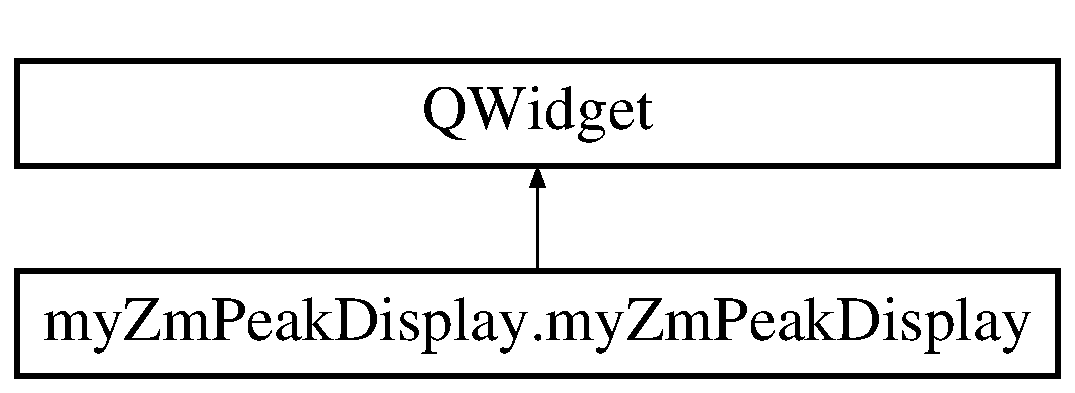
\includegraphics[height=2.000000cm]{classmyZmPeakDisplay_1_1myZmPeakDisplay}
\end{center}
\end{figure}
\subsection*{Public Member Functions}
\begin{DoxyCompactItemize}
\item 
\hypertarget{classmyZmPeakDisplay_1_1myZmPeakDisplay_a348a15b190a012ffee26f7526d2eca3c}{def {\bfseries \-\_\-\-\_\-init\-\_\-\-\_\-}}\label{classmyZmPeakDisplay_1_1myZmPeakDisplay_a348a15b190a012ffee26f7526d2eca3c}

\item 
\hypertarget{classmyZmPeakDisplay_1_1myZmPeakDisplay_aab9ac5a869bd132456f71fe022b2ad65}{def {\bfseries calc\-Histo}}\label{classmyZmPeakDisplay_1_1myZmPeakDisplay_aab9ac5a869bd132456f71fe022b2ad65}

\item 
\hypertarget{classmyZmPeakDisplay_1_1myZmPeakDisplay_a3a7fbef40f5613213deb5367a19f7857}{def {\bfseries set\-Min\-Max}}\label{classmyZmPeakDisplay_1_1myZmPeakDisplay_a3a7fbef40f5613213deb5367a19f7857}

\item 
\hypertarget{classmyZmPeakDisplay_1_1myZmPeakDisplay_af002add8e8eb6c55820cc2e12a8457c9}{def {\bfseries array\-To\-Q\-Image}}\label{classmyZmPeakDisplay_1_1myZmPeakDisplay_af002add8e8eb6c55820cc2e12a8457c9}

\item 
\hypertarget{classmyZmPeakDisplay_1_1myZmPeakDisplay_ae50e3adcca21aee551f8d757d77b9eba}{def {\bfseries write\-Q\-Image\-\_\-lut}}\label{classmyZmPeakDisplay_1_1myZmPeakDisplay_ae50e3adcca21aee551f8d757d77b9eba}

\item 
\hypertarget{classmyZmPeakDisplay_1_1myZmPeakDisplay_abd1762a6b6ac58060a7a3d5f2fc4ff1a}{def {\bfseries mouse\-Press\-Event}}\label{classmyZmPeakDisplay_1_1myZmPeakDisplay_abd1762a6b6ac58060a7a3d5f2fc4ff1a}

\item 
\hypertarget{classmyZmPeakDisplay_1_1myZmPeakDisplay_a7bce038050bb5bdd6b3d58be7ef13f00}{def {\bfseries mouse\-Release\-Event}}\label{classmyZmPeakDisplay_1_1myZmPeakDisplay_a7bce038050bb5bdd6b3d58be7ef13f00}

\item 
\hypertarget{classmyZmPeakDisplay_1_1myZmPeakDisplay_a86086ce776ea26bbb7c84dd6f49a3064}{def {\bfseries set\-Bar\-Flag}}\label{classmyZmPeakDisplay_1_1myZmPeakDisplay_a86086ce776ea26bbb7c84dd6f49a3064}

\item 
\hypertarget{classmyZmPeakDisplay_1_1myZmPeakDisplay_ada885fc1335a833a72ce8f65078c1fab}{def {\bfseries mouse\-Move\-Event}}\label{classmyZmPeakDisplay_1_1myZmPeakDisplay_ada885fc1335a833a72ce8f65078c1fab}

\item 
\hypertarget{classmyZmPeakDisplay_1_1myZmPeakDisplay_a86086ce776ea26bbb7c84dd6f49a3064}{def {\bfseries set\-Bar\-Flag}}\label{classmyZmPeakDisplay_1_1myZmPeakDisplay_a86086ce776ea26bbb7c84dd6f49a3064}

\item 
\hypertarget{classmyZmPeakDisplay_1_1myZmPeakDisplay_a45a5009c5ecc96d9a6ff350600478b37}{def {\bfseries paint\-Event}}\label{classmyZmPeakDisplay_1_1myZmPeakDisplay_a45a5009c5ecc96d9a6ff350600478b37}

\end{DoxyCompactItemize}
\subsection*{Public Attributes}
\begin{DoxyCompactItemize}
\item 
\hypertarget{classmyZmPeakDisplay_1_1myZmPeakDisplay_a2a58f32f3a30578f0d511a206dac4d92}{{\bfseries ind\-\_\-5}}\label{classmyZmPeakDisplay_1_1myZmPeakDisplay_a2a58f32f3a30578f0d511a206dac4d92}

\item 
\hypertarget{classmyZmPeakDisplay_1_1myZmPeakDisplay_a188042c43b850fa601b05ef9b45983b7}{{\bfseries ind\-\_\-95}}\label{classmyZmPeakDisplay_1_1myZmPeakDisplay_a188042c43b850fa601b05ef9b45983b7}

\item 
\hypertarget{classmyZmPeakDisplay_1_1myZmPeakDisplay_adc972d94702bf72b1aa7f9bafa51a523}{{\bfseries disp\-Max}}\label{classmyZmPeakDisplay_1_1myZmPeakDisplay_adc972d94702bf72b1aa7f9bafa51a523}

\item 
\hypertarget{classmyZmPeakDisplay_1_1myZmPeakDisplay_a82777e7574c238178144464a0a4c9dd5}{{\bfseries disp\-Min}}\label{classmyZmPeakDisplay_1_1myZmPeakDisplay_a82777e7574c238178144464a0a4c9dd5}

\item 
\hypertarget{classmyZmPeakDisplay_1_1myZmPeakDisplay_a4d79fa930b80664bf9c661c69c90e45a}{{\bfseries scale}}\label{classmyZmPeakDisplay_1_1myZmPeakDisplay_a4d79fa930b80664bf9c661c69c90e45a}

\item 
\hypertarget{classmyZmPeakDisplay_1_1myZmPeakDisplay_ac30db7d7e88a260a660c73842cc7e70c}{{\bfseries newx}}\label{classmyZmPeakDisplay_1_1myZmPeakDisplay_ac30db7d7e88a260a660c73842cc7e70c}

\item 
\hypertarget{classmyZmPeakDisplay_1_1myZmPeakDisplay_aa5d3657333093135e384f3bfa49a9ddf}{{\bfseries newy}}\label{classmyZmPeakDisplay_1_1myZmPeakDisplay_aa5d3657333093135e384f3bfa49a9ddf}

\item 
\hypertarget{classmyZmPeakDisplay_1_1myZmPeakDisplay_a1ff0a93d46b719217c98326afd23efc0}{{\bfseries qimage}}\label{classmyZmPeakDisplay_1_1myZmPeakDisplay_a1ff0a93d46b719217c98326afd23efc0}

\item 
\hypertarget{classmyZmPeakDisplay_1_1myZmPeakDisplay_a90d2173fc5c4bda615e1f6e2cda08d89}{{\bfseries load\-Image}}\label{classmyZmPeakDisplay_1_1myZmPeakDisplay_a90d2173fc5c4bda615e1f6e2cda08d89}

\item 
\hypertarget{classmyZmPeakDisplay_1_1myZmPeakDisplay_a72f7fc0519471f766cacc379811b3de0}{{\bfseries startx}}\label{classmyZmPeakDisplay_1_1myZmPeakDisplay_a72f7fc0519471f766cacc379811b3de0}

\item 
\hypertarget{classmyZmPeakDisplay_1_1myZmPeakDisplay_a18be92130080c324da24bfd8bb70d1f0}{{\bfseries starty}}\label{classmyZmPeakDisplay_1_1myZmPeakDisplay_a18be92130080c324da24bfd8bb70d1f0}

\item 
\hypertarget{classmyZmPeakDisplay_1_1myZmPeakDisplay_ad5645653988974bebc739532eac8ef86}{{\bfseries ns}}\label{classmyZmPeakDisplay_1_1myZmPeakDisplay_ad5645653988974bebc739532eac8ef86}

\item 
\hypertarget{classmyZmPeakDisplay_1_1myZmPeakDisplay_aa08f61c355a9ebaf1ee628a10ba72a02}{{\bfseries nl}}\label{classmyZmPeakDisplay_1_1myZmPeakDisplay_aa08f61c355a9ebaf1ee628a10ba72a02}

\item 
\hypertarget{classmyZmPeakDisplay_1_1myZmPeakDisplay_a3418f94ca8d8f74f38e83a9857cacd5b}{{\bfseries zm\-Fac}}\label{classmyZmPeakDisplay_1_1myZmPeakDisplay_a3418f94ca8d8f74f38e83a9857cacd5b}

\item 
\hypertarget{classmyZmPeakDisplay_1_1myZmPeakDisplay_ae1ca848339601ec3d5cdd9409a683ce9}{{\bfseries vbarloc}}\label{classmyZmPeakDisplay_1_1myZmPeakDisplay_ae1ca848339601ec3d5cdd9409a683ce9}

\item 
\hypertarget{classmyZmPeakDisplay_1_1myZmPeakDisplay_ad44f714b1fc1fc724d16ebdb4d910574}{{\bfseries hbarloc}}\label{classmyZmPeakDisplay_1_1myZmPeakDisplay_ad44f714b1fc1fc724d16ebdb4d910574}

\item 
\hypertarget{classmyZmPeakDisplay_1_1myZmPeakDisplay_adf7a9d7f5ca82215805acbc121e9d42d}{{\bfseries vbarloc\-\_\-orig}}\label{classmyZmPeakDisplay_1_1myZmPeakDisplay_adf7a9d7f5ca82215805acbc121e9d42d}

\item 
\hypertarget{classmyZmPeakDisplay_1_1myZmPeakDisplay_a9f46ba18c0baa95bd2c7ec8b70dcddbe}{{\bfseries hbarloc\-\_\-orig}}\label{classmyZmPeakDisplay_1_1myZmPeakDisplay_a9f46ba18c0baa95bd2c7ec8b70dcddbe}

\item 
\hypertarget{classmyZmPeakDisplay_1_1myZmPeakDisplay_a2ad52ce54407b62ce8829e538a845049}{{\bfseries fulldata}}\label{classmyZmPeakDisplay_1_1myZmPeakDisplay_a2ad52ce54407b62ce8829e538a845049}

\item 
\hypertarget{classmyZmPeakDisplay_1_1myZmPeakDisplay_aead8ab13c78f41a35434760be199264a}{{\bfseries zoom\-Rect}}\label{classmyZmPeakDisplay_1_1myZmPeakDisplay_aead8ab13c78f41a35434760be199264a}

\item 
\hypertarget{classmyZmPeakDisplay_1_1myZmPeakDisplay_ab0a84e7b6930d7b42d51c4bc0a2fc4ec}{{\bfseries bar\-Flag}}\label{classmyZmPeakDisplay_1_1myZmPeakDisplay_ab0a84e7b6930d7b42d51c4bc0a2fc4ec}

\end{DoxyCompactItemize}
\subsection*{Static Public Attributes}
\begin{DoxyCompactItemize}
\item 
\hypertarget{classmyZmPeakDisplay_1_1myZmPeakDisplay_a52a6206bea396c772d3c3f3bd9e39263}{int {\bfseries load\-Image} = 0}\label{classmyZmPeakDisplay_1_1myZmPeakDisplay_a52a6206bea396c772d3c3f3bd9e39263}

\item 
\hypertarget{classmyZmPeakDisplay_1_1myZmPeakDisplay_a513bd49e45f862ce6d675c0fd1403d1a}{int {\bfseries disp\-Max} = 1000}\label{classmyZmPeakDisplay_1_1myZmPeakDisplay_a513bd49e45f862ce6d675c0fd1403d1a}

\item 
\hypertarget{classmyZmPeakDisplay_1_1myZmPeakDisplay_aaee145150aa3dc3ec84d322d1361fc9d}{int {\bfseries disp\-Min} = 0}\label{classmyZmPeakDisplay_1_1myZmPeakDisplay_aaee145150aa3dc3ec84d322d1361fc9d}

\item 
\hypertarget{classmyZmPeakDisplay_1_1myZmPeakDisplay_af5ac7ba7a7d3b83223b61462349f6d46}{int {\bfseries zm\-Fac} = 4}\label{classmyZmPeakDisplay_1_1myZmPeakDisplay_af5ac7ba7a7d3b83223b61462349f6d46}

\item 
\hypertarget{classmyZmPeakDisplay_1_1myZmPeakDisplay_a61900777c8f1ee16eefca8614f7a940c}{int {\bfseries newx} = 0}\label{classmyZmPeakDisplay_1_1myZmPeakDisplay_a61900777c8f1ee16eefca8614f7a940c}

\item 
\hypertarget{classmyZmPeakDisplay_1_1myZmPeakDisplay_ac6ef82ef45e92d1380a4122b085933e6}{int {\bfseries newy} = 0}\label{classmyZmPeakDisplay_1_1myZmPeakDisplay_ac6ef82ef45e92d1380a4122b085933e6}

\item 
\hypertarget{classmyZmPeakDisplay_1_1myZmPeakDisplay_a76602f7e8c11dbd816a9161b0a864ccd}{int {\bfseries ns} = 21}\label{classmyZmPeakDisplay_1_1myZmPeakDisplay_a76602f7e8c11dbd816a9161b0a864ccd}

\item 
\hypertarget{classmyZmPeakDisplay_1_1myZmPeakDisplay_a98ac7ad822c6d740e6a748b1dabb96b5}{int {\bfseries nl} = 21}\label{classmyZmPeakDisplay_1_1myZmPeakDisplay_a98ac7ad822c6d740e6a748b1dabb96b5}

\item 
\hypertarget{classmyZmPeakDisplay_1_1myZmPeakDisplay_ac2ffc7ced35826e8eed43f5abbf0e3d0}{{\bfseries zoom\-Toggle} = True}\label{classmyZmPeakDisplay_1_1myZmPeakDisplay_ac2ffc7ced35826e8eed43f5abbf0e3d0}

\item 
\hypertarget{classmyZmPeakDisplay_1_1myZmPeakDisplay_a4a28127e7e5fa8bab3d21c4693d7fede}{{\bfseries peak\-Toggle} = False}\label{classmyZmPeakDisplay_1_1myZmPeakDisplay_a4a28127e7e5fa8bab3d21c4693d7fede}

\item 
\hypertarget{classmyZmPeakDisplay_1_1myZmPeakDisplay_a43b75e7b7d508ce23a9f4e663917fa01}{tuple {\bfseries zoom\-Rect} = Qt\-Core.\-Q\-Rect()}\label{classmyZmPeakDisplay_1_1myZmPeakDisplay_a43b75e7b7d508ce23a9f4e663917fa01}

\item 
\hypertarget{classmyZmPeakDisplay_1_1myZmPeakDisplay_ac88fb195fd24548062bf22107b9dfa18}{int {\bfseries bar\-Flag} = 1}\label{classmyZmPeakDisplay_1_1myZmPeakDisplay_ac88fb195fd24548062bf22107b9dfa18}

\item 
\hypertarget{classmyZmPeakDisplay_1_1myZmPeakDisplay_a297952d3c6546ef718feb343566fe283}{{\bfseries bar\-Drag} = False}\label{classmyZmPeakDisplay_1_1myZmPeakDisplay_a297952d3c6546ef718feb343566fe283}

\item 
\hypertarget{classmyZmPeakDisplay_1_1myZmPeakDisplay_ad44d50518d3ab0f2eb9c3ddb0d247906}{int {\bfseries vbarloc} = ns/2}\label{classmyZmPeakDisplay_1_1myZmPeakDisplay_ad44d50518d3ab0f2eb9c3ddb0d247906}

\item 
\hypertarget{classmyZmPeakDisplay_1_1myZmPeakDisplay_a27608279f98a23a7c3c869df0d3995ce}{int {\bfseries hbarloc} = nl/2}\label{classmyZmPeakDisplay_1_1myZmPeakDisplay_a27608279f98a23a7c3c869df0d3995ce}

\item 
\hypertarget{classmyZmPeakDisplay_1_1myZmPeakDisplay_adff5c6da641109f0677fa397b0a3331d}{int {\bfseries startx} = 0}\label{classmyZmPeakDisplay_1_1myZmPeakDisplay_adff5c6da641109f0677fa397b0a3331d}

\item 
\hypertarget{classmyZmPeakDisplay_1_1myZmPeakDisplay_a149e621976069c20cd89545890f708ea}{int {\bfseries starty} = 0}\label{classmyZmPeakDisplay_1_1myZmPeakDisplay_a149e621976069c20cd89545890f708ea}

\item 
\hypertarget{classmyZmPeakDisplay_1_1myZmPeakDisplay_acb4b811dcb4c35efd8dcedcccd1050db}{tuple {\bfseries slide\-Bar\-Signal} = Qt\-Core.\-pyqt\-Signal(int, int, int)}\label{classmyZmPeakDisplay_1_1myZmPeakDisplay_acb4b811dcb4c35efd8dcedcccd1050db}

\item 
\hypertarget{classmyZmPeakDisplay_1_1myZmPeakDisplay_add6e28bc8fcf22321234c3c76090d0b4}{{\bfseries raw\-Arr} = None}\label{classmyZmPeakDisplay_1_1myZmPeakDisplay_add6e28bc8fcf22321234c3c76090d0b4}

\end{DoxyCompactItemize}


The documentation for this class was generated from the following file\-:\begin{DoxyCompactItemize}
\item 
/home/harold/workdir/atrex/\-Software/my\-Zm\-Peak\-Display.\-py\end{DoxyCompactItemize}

\hypertarget{classtifffile_1_1TiffSequence_1_1ParseError}{\section{tifffile.\-Tiff\-Sequence.\-Parse\-Error Class Reference}
\label{classtifffile_1_1TiffSequence_1_1ParseError}\index{tifffile.\-Tiff\-Sequence.\-Parse\-Error@{tifffile.\-Tiff\-Sequence.\-Parse\-Error}}
}
Inheritance diagram for tifffile.\-Tiff\-Sequence.\-Parse\-Error\-:\begin{figure}[H]
\begin{center}
\leavevmode
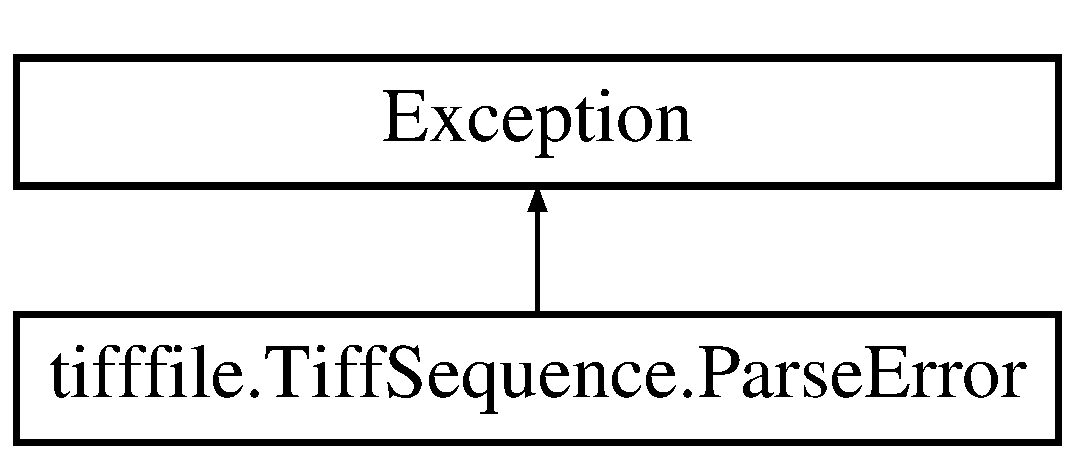
\includegraphics[height=2.000000cm]{classtifffile_1_1TiffSequence_1_1ParseError}
\end{center}
\end{figure}


The documentation for this class was generated from the following file\-:\begin{DoxyCompactItemize}
\item 
/home/harold/workdir/atrex/\-Software/tifffile.\-py\end{DoxyCompactItemize}

\hypertarget{classpeakEditDlg_1_1peakEditDlg}{\section{peak\-Edit\-Dlg.\-peak\-Edit\-Dlg Class Reference}
\label{classpeakEditDlg_1_1peakEditDlg}\index{peak\-Edit\-Dlg.\-peak\-Edit\-Dlg@{peak\-Edit\-Dlg.\-peak\-Edit\-Dlg}}
}
Inheritance diagram for peak\-Edit\-Dlg.\-peak\-Edit\-Dlg\-:\begin{figure}[H]
\begin{center}
\leavevmode
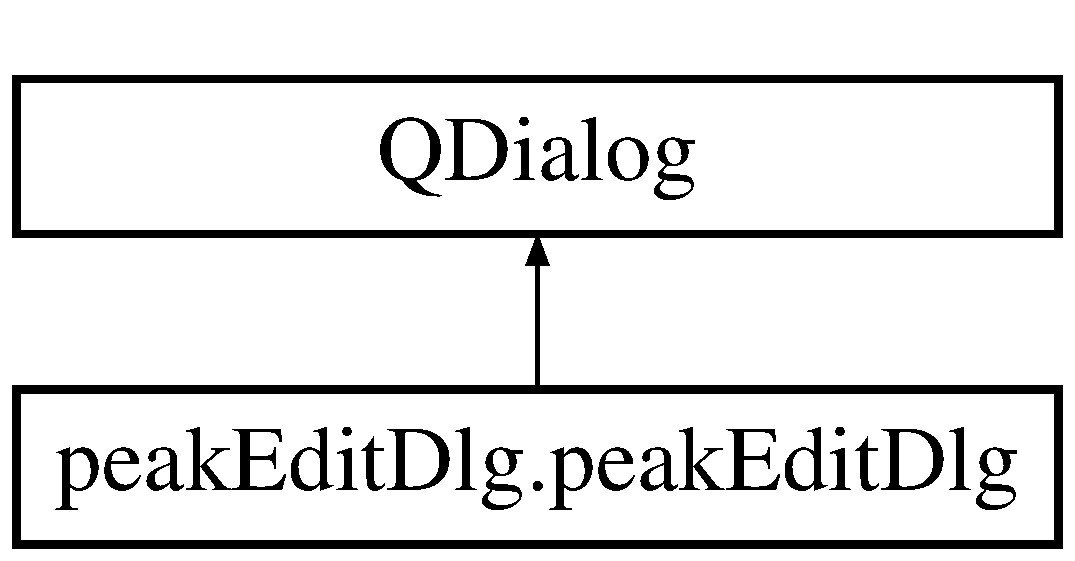
\includegraphics[height=2.000000cm]{classpeakEditDlg_1_1peakEditDlg}
\end{center}
\end{figure}
\subsection*{Public Member Functions}
\begin{DoxyCompactItemize}
\item 
\hypertarget{classpeakEditDlg_1_1peakEditDlg_a3a89be502d41175fb5b75fd419715096}{def {\bfseries \-\_\-\-\_\-init\-\_\-\-\_\-}}\label{classpeakEditDlg_1_1peakEditDlg_a3a89be502d41175fb5b75fd419715096}

\item 
\hypertarget{classpeakEditDlg_1_1peakEditDlg_ab11967324093e3350fe404fa29e255c1}{def {\bfseries set\-Image\-File}}\label{classpeakEditDlg_1_1peakEditDlg_ab11967324093e3350fe404fa29e255c1}

\item 
\hypertarget{classpeakEditDlg_1_1peakEditDlg_a2f577ff67c33813f4d803e5d85e62eb2}{def {\bfseries text\-Set\-D}}\label{classpeakEditDlg_1_1peakEditDlg_a2f577ff67c33813f4d803e5d85e62eb2}

\item 
\hypertarget{classpeakEditDlg_1_1peakEditDlg_a2dc064d39d748e09a70a7f6a236c7187}{def {\bfseries text\-Set\-F}}\label{classpeakEditDlg_1_1peakEditDlg_a2dc064d39d748e09a70a7f6a236c7187}

\end{DoxyCompactItemize}
\subsection*{Public Attributes}
\begin{DoxyCompactItemize}
\item 
\hypertarget{classpeakEditDlg_1_1peakEditDlg_a0220ea9f1c4703a47098891c57e1da1f}{{\bfseries ui}}\label{classpeakEditDlg_1_1peakEditDlg_a0220ea9f1c4703a47098891c57e1da1f}

\item 
\hypertarget{classpeakEditDlg_1_1peakEditDlg_abd94cfb1dd7a9ed84e1955b100a0be78}{{\bfseries peak}}\label{classpeakEditDlg_1_1peakEditDlg_abd94cfb1dd7a9ed84e1955b100a0be78}

\end{DoxyCompactItemize}


The documentation for this class was generated from the following file\-:\begin{DoxyCompactItemize}
\item 
/home/harold/workdir/atrex/\-Software/peak\-Edit\-Dlg.\-py\end{DoxyCompactItemize}

\hypertarget{classpeakFit_1_1peakFit}{\section{peak\-Fit.\-peak\-Fit Class Reference}
\label{classpeakFit_1_1peakFit}\index{peak\-Fit.\-peak\-Fit@{peak\-Fit.\-peak\-Fit}}
}
\subsection*{Public Member Functions}
\begin{DoxyCompactItemize}
\item 
\hypertarget{classpeakFit_1_1peakFit_a6ab39ce33c91775176e0c46cc6f936f6}{def {\bfseries \-\_\-\-\_\-init\-\_\-\-\_\-}}\label{classpeakFit_1_1peakFit_a6ab39ce33c91775176e0c46cc6f936f6}

\item 
\hypertarget{classpeakFit_1_1peakFit_a84a91a33d88ca2403a4e435b5d1f90ec}{def {\bfseries fit\-Arr}}\label{classpeakFit_1_1peakFit_a84a91a33d88ca2403a4e435b5d1f90ec}

\item 
\hypertarget{classpeakFit_1_1peakFit_a0bbfae3ae35fbad87477c06b1607362a}{def {\bfseries fit\-Array}}\label{classpeakFit_1_1peakFit_a0bbfae3ae35fbad87477c06b1607362a}

\item 
\hypertarget{classpeakFit_1_1peakFit_a4be5cc7b519e08cd3c401e44449ff06b}{def {\bfseries return\-Fit\-Array}}\label{classpeakFit_1_1peakFit_a4be5cc7b519e08cd3c401e44449ff06b}

\item 
\hypertarget{classpeakFit_1_1peakFit_ad2af816ebe4e711d783eac36caf062fd}{def {\bfseries return\-Fit}}\label{classpeakFit_1_1peakFit_ad2af816ebe4e711d783eac36caf062fd}

\item 
\hypertarget{classpeakFit_1_1peakFit_a430b52fc42d7539b1374dc4bd1b64efc}{def {\bfseries interp\-Array}}\label{classpeakFit_1_1peakFit_a430b52fc42d7539b1374dc4bd1b64efc}

\end{DoxyCompactItemize}
\subsection*{Public Attributes}
\begin{DoxyCompactItemize}
\item 
\hypertarget{classpeakFit_1_1peakFit_a46bbd242120c1eb44158673fc1ba69eb}{{\bfseries inarr}}\label{classpeakFit_1_1peakFit_a46bbd242120c1eb44158673fc1ba69eb}

\item 
\hypertarget{classpeakFit_1_1peakFit_a7bcef9f3d5dbca4a5470a53661dabe4c}{{\bfseries fitpars}}\label{classpeakFit_1_1peakFit_a7bcef9f3d5dbca4a5470a53661dabe4c}

\item 
\hypertarget{classpeakFit_1_1peakFit_a1d06c78ecd07718ae71cc50df4d0251c}{{\bfseries fitted}}\label{classpeakFit_1_1peakFit_a1d06c78ecd07718ae71cc50df4d0251c}

\end{DoxyCompactItemize}


The documentation for this class was generated from the following file\-:\begin{DoxyCompactItemize}
\item 
/home/harold/workdir/atrex/\-Software/peak\-Fit.\-py\end{DoxyCompactItemize}

\hypertarget{classPeakObject_1_1PeakObject}{\section{Peak\-Object.\-Peak\-Object Class Reference}
\label{classPeakObject_1_1PeakObject}\index{Peak\-Object.\-Peak\-Object@{Peak\-Object.\-Peak\-Object}}
}
\subsection*{Public Member Functions}
\begin{DoxyCompactItemize}
\item 
\hypertarget{classPeakObject_1_1PeakObject_a066c72d23958912081182a5aca95e32c}{def {\bfseries \-\_\-\-\_\-init\-\_\-\-\_\-}}\label{classPeakObject_1_1PeakObject_a066c72d23958912081182a5aca95e32c}

\item 
\hypertarget{classPeakObject_1_1PeakObject_a44e1f82c79582b10885050ae8ffd7201}{def {\bfseries x}}\label{classPeakObject_1_1PeakObject_a44e1f82c79582b10885050ae8ffd7201}

\item 
\hypertarget{classPeakObject_1_1PeakObject_a674a319850462abc76a7091e49c2425c}{def {\bfseries y}}\label{classPeakObject_1_1PeakObject_a674a319850462abc76a7091e49c2425c}

\item 
\hypertarget{classPeakObject_1_1PeakObject_a4a9dabf7ebe3b0703da235f77259d5d2}{def {\bfseries set\-Selected}}\label{classPeakObject_1_1PeakObject_a4a9dabf7ebe3b0703da235f77259d5d2}

\end{DoxyCompactItemize}
\subsection*{Public Attributes}
\begin{DoxyCompactItemize}
\item 
\hypertarget{classPeakObject_1_1PeakObject_a0675bfef330cb0e7111c507d0fd2f505}{{\bfseries xloc}}\label{classPeakObject_1_1PeakObject_a0675bfef330cb0e7111c507d0fd2f505}

\item 
\hypertarget{classPeakObject_1_1PeakObject_adc5441b9bde0d002725032741bce8a3a}{{\bfseries yloc}}\label{classPeakObject_1_1PeakObject_adc5441b9bde0d002725032741bce8a3a}

\end{DoxyCompactItemize}
\subsection*{Static Public Attributes}
\begin{DoxyCompactItemize}
\item 
\hypertarget{classPeakObject_1_1PeakObject_a547374a82aab09bcf28e13ecfb598117}{int {\bfseries xloc} = 0}\label{classPeakObject_1_1PeakObject_a547374a82aab09bcf28e13ecfb598117}

\item 
\hypertarget{classPeakObject_1_1PeakObject_abebfb4985f9b0b73e6b1e20cb5a56f18}{int {\bfseries yloc} = 0}\label{classPeakObject_1_1PeakObject_abebfb4985f9b0b73e6b1e20cb5a56f18}

\item 
\hypertarget{classPeakObject_1_1PeakObject_a5d69241780c9ba49bccd1a76c3ef2738}{tuple {\bfseries ident} = Qt\-Core.\-Q\-String(\char`\"{}\char`\"{})}\label{classPeakObject_1_1PeakObject_a5d69241780c9ba49bccd1a76c3ef2738}

\item 
\hypertarget{classPeakObject_1_1PeakObject_aa0095eabde0eeb9ed146a052f7dea921}{{\bfseries selected} = False}\label{classPeakObject_1_1PeakObject_aa0095eabde0eeb9ed146a052f7dea921}

\end{DoxyCompactItemize}


The documentation for this class was generated from the following file\-:\begin{DoxyCompactItemize}
\item 
/home/harold/workdir/atrex/\-Software/Peak\-Object.\-py\end{DoxyCompactItemize}

\hypertarget{classProject_1_1Project}{\section{Project.\-Project Class Reference}
\label{classProject_1_1Project}\index{Project.\-Project@{Project.\-Project}}
}
\subsection*{Public Member Functions}
\begin{DoxyCompactItemize}
\item 
\hypertarget{classProject_1_1Project_a59b578ef2b746c294bee8d2ceb8ea3d9}{def {\bfseries \-\_\-\-\_\-init\-\_\-\-\_\-}}\label{classProject_1_1Project_a59b578ef2b746c294bee8d2ceb8ea3d9}

\item 
def \hyperlink{classProject_1_1Project_af5d15337a24279fed5df943cdd17a521}{get\-Image\-Base}
\item 
\hypertarget{classProject_1_1Project_af4f0a9adbac70beed61838e0552b5fce}{def {\bfseries get\-File\-Name\-From\-Num}}\label{classProject_1_1Project_af4f0a9adbac70beed61838e0552b5fce}

\item 
\hypertarget{classProject_1_1Project_a26e3cfe3e056c97f722eeef03137c475}{def {\bfseries get\-File\-Number}}\label{classProject_1_1Project_a26e3cfe3e056c97f722eeef03137c475}

\item 
\hypertarget{classProject_1_1Project_aa4241d0e834f8686b89e977ad6b16d26}{def {\bfseries check\-For\-Files}}\label{classProject_1_1Project_aa4241d0e834f8686b89e977ad6b16d26}

\item 
\hypertarget{classProject_1_1Project_abcb28ed447f9094e8eb6d6a49b0c4294}{def {\bfseries read\-File\-Settings}}\label{classProject_1_1Project_abcb28ed447f9094e8eb6d6a49b0c4294}

\item 
\hypertarget{classProject_1_1Project_a4b58bd09e8457006fb81aa85d7723a7d}{def {\bfseries write\-Settings\-Files}}\label{classProject_1_1Project_a4b58bd09e8457006fb81aa85d7723a7d}

\end{DoxyCompactItemize}
\subsection*{Public Attributes}
\begin{DoxyCompactItemize}
\item 
\hypertarget{classProject_1_1Project_ad80180beff6260cee514b29e80083d55}{{\bfseries ub\-Flag}}\label{classProject_1_1Project_ad80180beff6260cee514b29e80083d55}

\item 
\hypertarget{classProject_1_1Project_a057b409d634c343f346408dbf90a8eeb}{{\bfseries cal\-Flag}}\label{classProject_1_1Project_a057b409d634c343f346408dbf90a8eeb}

\item 
\hypertarget{classProject_1_1Project_a6faaef14edf4c340f2006ea4ce7ce5d9}{{\bfseries proj\-File}}\label{classProject_1_1Project_a6faaef14edf4c340f2006ea4ce7ce5d9}

\item 
\hypertarget{classProject_1_1Project_a8eae8faddab323b07537ca6a5f3916cc}{{\bfseries ub\-File}}\label{classProject_1_1Project_a8eae8faddab323b07537ca6a5f3916cc}

\item 
\hypertarget{classProject_1_1Project_ad75bb22fb985bf29b7f9bd2560b871a5}{{\bfseries cal\-File}}\label{classProject_1_1Project_ad75bb22fb985bf29b7f9bd2560b871a5}

\item 
\hypertarget{classProject_1_1Project_a06b77a0f6c41da2453cfce4cb5e6a05d}{{\bfseries settings\-Array}}\label{classProject_1_1Project_a06b77a0f6c41da2453cfce4cb5e6a05d}

\item 
\hypertarget{classProject_1_1Project_ae8e5eb7ce2196fd5eec5b91686732069}{{\bfseries filenum}}\label{classProject_1_1Project_ae8e5eb7ce2196fd5eec5b91686732069}

\item 
\hypertarget{classProject_1_1Project_a5e0248c4f5f2a4c91daaad537afa060c}{{\bfseries curimage}}\label{classProject_1_1Project_a5e0248c4f5f2a4c91daaad537afa060c}

\item 
\hypertarget{classProject_1_1Project_a24e1a52b21994951813562a80bfcdcad}{{\bfseries proj\-Flag}}\label{classProject_1_1Project_a24e1a52b21994951813562a80bfcdcad}

\item 
\hypertarget{classProject_1_1Project_abf36ec5e3005385e03d533200b5c098a}{{\bfseries num\-Digits}}\label{classProject_1_1Project_abf36ec5e3005385e03d533200b5c098a}

\item 
\hypertarget{classProject_1_1Project_aec70e48d90635d6c41b66660fc23c14b}{{\bfseries im\-File}}\label{classProject_1_1Project_aec70e48d90635d6c41b66660fc23c14b}

\item 
\hypertarget{classProject_1_1Project_ae2e3e43c456a03959ddc60f010e54aa9}{{\bfseries omega0}}\label{classProject_1_1Project_ae2e3e43c456a03959ddc60f010e54aa9}

\item 
\hypertarget{classProject_1_1Project_a05d50a418a51ea0f4dcf7d1a87812b00}{{\bfseries omega\-R}}\label{classProject_1_1Project_a05d50a418a51ea0f4dcf7d1a87812b00}

\item 
\hypertarget{classProject_1_1Project_aa53e83e0b9b4b05e86bbb6b80873d700}{{\bfseries expos}}\label{classProject_1_1Project_aa53e83e0b9b4b05e86bbb6b80873d700}

\item 
\hypertarget{classProject_1_1Project_aae1d33efbce822c8023528ff7f3b841a}{{\bfseries chi}}\label{classProject_1_1Project_aae1d33efbce822c8023528ff7f3b841a}

\item 
\hypertarget{classProject_1_1Project_a2513615e3adc838e60e00da5c77ef307}{{\bfseries detector}}\label{classProject_1_1Project_a2513615e3adc838e60e00da5c77ef307}

\item 
\hypertarget{classProject_1_1Project_a4a1a26e41d50eafb9a1ecd7c344ae974}{{\bfseries base}}\label{classProject_1_1Project_a4a1a26e41d50eafb9a1ecd7c344ae974}

\item 
\hypertarget{classProject_1_1Project_a1ca86041217dfdbb3a7d0e626181dd74}{{\bfseries h5\-Flag}}\label{classProject_1_1Project_a1ca86041217dfdbb3a7d0e626181dd74}

\item 
\hypertarget{classProject_1_1Project_af03d34654b00a3f4d1f8a38b834af406}{{\bfseries min\-Image\-Num}}\label{classProject_1_1Project_af03d34654b00a3f4d1f8a38b834af406}

\item 
\hypertarget{classProject_1_1Project_afc5b3afcc2020e4527c6328c508ad5c9}{{\bfseries max\-Image\-Num}}\label{classProject_1_1Project_afc5b3afcc2020e4527c6328c508ad5c9}

\item 
\hypertarget{classProject_1_1Project_a7faf083a4e6924fd1abe50b00ffe2c7d}{{\bfseries num\-Images}}\label{classProject_1_1Project_a7faf083a4e6924fd1abe50b00ffe2c7d}

\item 
\hypertarget{classProject_1_1Project_aed74c6fd1832b33e1299f1180a691fa6}{{\bfseries prj\-File}}\label{classProject_1_1Project_aed74c6fd1832b33e1299f1180a691fa6}

\end{DoxyCompactItemize}


\subsection{Detailed Description}
\begin{DoxyVerb}Project.py
Class containing utilities to get the image base from a input file name and to return a filename
based upon the image base
\end{DoxyVerb}
 

\subsection{Member Function Documentation}
\hypertarget{classProject_1_1Project_af5d15337a24279fed5df943cdd17a521}{\index{Project\-::\-Project@{Project\-::\-Project}!get\-Image\-Base@{get\-Image\-Base}}
\index{get\-Image\-Base@{get\-Image\-Base}!Project::Project@{Project\-::\-Project}}
\subsubsection[{get\-Image\-Base}]{\setlength{\rightskip}{0pt plus 5cm}def Project.\-Project.\-get\-Image\-Base (
\begin{DoxyParamCaption}
\item[{}]{self, }
\item[{}]{filename}
\end{DoxyParamCaption}
)}}\label{classProject_1_1Project_af5d15337a24279fed5df943cdd17a521}
\begin{DoxyVerb}getImageBase returns the prefix which will be used for subsequent file naming based upon
an input filename
:param filename:
:return:
\end{DoxyVerb}
 

The documentation for this class was generated from the following file\-:\begin{DoxyCompactItemize}
\item 
/home/harold/workdir/atrex/\-Software/Project.\-py\end{DoxyCompactItemize}

\hypertarget{classtifffile_1_1Record}{\section{tifffile.\-Record Class Reference}
\label{classtifffile_1_1Record}\index{tifffile.\-Record@{tifffile.\-Record}}
}
Inheritance diagram for tifffile.\-Record\-:\begin{figure}[H]
\begin{center}
\leavevmode
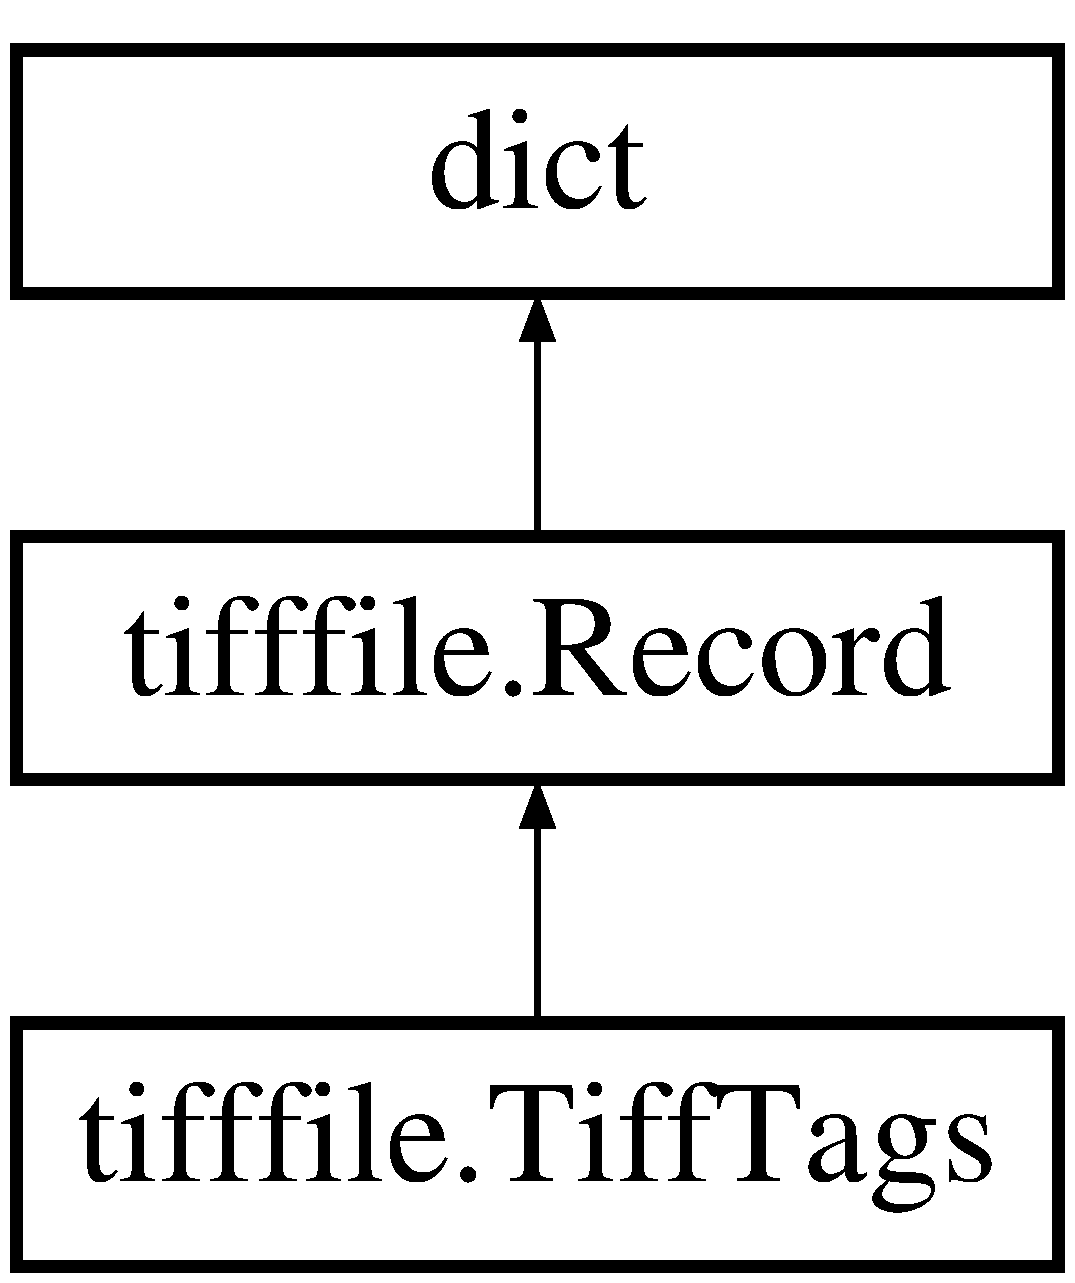
\includegraphics[height=3.000000cm]{classtifffile_1_1Record}
\end{center}
\end{figure}
\subsection*{Public Member Functions}
\begin{DoxyCompactItemize}
\item 
\hypertarget{classtifffile_1_1Record_a0ff543c8d9ef139ba868177e0db7ac02}{def {\bfseries \-\_\-\-\_\-init\-\_\-\-\_\-}}\label{classtifffile_1_1Record_a0ff543c8d9ef139ba868177e0db7ac02}

\item 
\hypertarget{classtifffile_1_1Record_aeba3dd18a66ecb80f9d6fc09dae33a5d}{def {\bfseries \-\_\-\-\_\-getattr\-\_\-\-\_\-}}\label{classtifffile_1_1Record_aeba3dd18a66ecb80f9d6fc09dae33a5d}

\item 
\hypertarget{classtifffile_1_1Record_a2fc93e114d60c64619cd6ea297c186bf}{def {\bfseries \-\_\-\-\_\-setattr\-\_\-\-\_\-}}\label{classtifffile_1_1Record_a2fc93e114d60c64619cd6ea297c186bf}

\item 
def \hyperlink{classtifffile_1_1Record_a6462a5901c01bd8644032e4c55005e57}{\-\_\-\-\_\-str\-\_\-\-\_\-}
\end{DoxyCompactItemize}


\subsection{Detailed Description}
\begin{DoxyVerb}Dictionary with attribute access.

Can also be initialized with numpy.core.records.record.\end{DoxyVerb}
 

\subsection{Member Function Documentation}
\hypertarget{classtifffile_1_1Record_a6462a5901c01bd8644032e4c55005e57}{\index{tifffile\-::\-Record@{tifffile\-::\-Record}!\-\_\-\-\_\-str\-\_\-\-\_\-@{\-\_\-\-\_\-str\-\_\-\-\_\-}}
\index{\-\_\-\-\_\-str\-\_\-\-\_\-@{\-\_\-\-\_\-str\-\_\-\-\_\-}!tifffile::Record@{tifffile\-::\-Record}}
\subsubsection[{\-\_\-\-\_\-str\-\_\-\-\_\-}]{\setlength{\rightskip}{0pt plus 5cm}def tifffile.\-Record.\-\_\-\-\_\-str\-\_\-\-\_\- (
\begin{DoxyParamCaption}
\item[{}]{self}
\end{DoxyParamCaption}
)}}\label{classtifffile_1_1Record_a6462a5901c01bd8644032e4c55005e57}
\begin{DoxyVerb}Pretty print Record.\end{DoxyVerb}
 

The documentation for this class was generated from the following file\-:\begin{DoxyCompactItemize}
\item 
/home/harold/workdir/atrex/\-Software/tifffile.\-py\end{DoxyCompactItemize}

\hypertarget{classJCPDS_1_1Reflection}{\section{J\-C\-P\-D\-S.\-Reflection Class Reference}
\label{classJCPDS_1_1Reflection}\index{J\-C\-P\-D\-S.\-Reflection@{J\-C\-P\-D\-S.\-Reflection}}
}
\subsection*{Public Member Functions}
\begin{DoxyCompactItemize}
\item 
\hypertarget{classJCPDS_1_1Reflection_a60f239e7b0dc01ae22859aab4ce15958}{def {\bfseries parse\-Vals}}\label{classJCPDS_1_1Reflection_a60f239e7b0dc01ae22859aab4ce15958}

\item 
\hypertarget{classJCPDS_1_1Reflection_a5b0c369390f0f6c9d4f43f79451666ad}{def {\bfseries parse\-Vals\-X\-P\-O\-W}}\label{classJCPDS_1_1Reflection_a5b0c369390f0f6c9d4f43f79451666ad}

\end{DoxyCompactItemize}
\subsection*{Public Attributes}
\begin{DoxyCompactItemize}
\item 
\hypertarget{classJCPDS_1_1Reflection_a2e19b84f40e3e5dadbe49a60cd45406e}{{\bfseries d0}}\label{classJCPDS_1_1Reflection_a2e19b84f40e3e5dadbe49a60cd45406e}

\item 
\hypertarget{classJCPDS_1_1Reflection_af4298638f38bd63f0731ee0d564f390d}{{\bfseries inten}}\label{classJCPDS_1_1Reflection_af4298638f38bd63f0731ee0d564f390d}

\item 
\hypertarget{classJCPDS_1_1Reflection_aaab66547bee474122bb66caa9732b683}{{\bfseries h}}\label{classJCPDS_1_1Reflection_aaab66547bee474122bb66caa9732b683}

\item 
\hypertarget{classJCPDS_1_1Reflection_a40102fb28adbda5bc337211845a3a3e3}{{\bfseries k}}\label{classJCPDS_1_1Reflection_a40102fb28adbda5bc337211845a3a3e3}

\item 
\hypertarget{classJCPDS_1_1Reflection_a678d14a1fe67331931242cc73ef096b9}{{\bfseries l}}\label{classJCPDS_1_1Reflection_a678d14a1fe67331931242cc73ef096b9}

\end{DoxyCompactItemize}
\subsection*{Static Public Attributes}
\begin{DoxyCompactItemize}
\item 
\hypertarget{classJCPDS_1_1Reflection_a21cdd847ccc4a67939ba0f7eddb288b5}{int {\bfseries d0} = 0}\label{classJCPDS_1_1Reflection_a21cdd847ccc4a67939ba0f7eddb288b5}

\item 
\hypertarget{classJCPDS_1_1Reflection_a343546653e0fa7aa59c9ef63366d6d95}{int {\bfseries d} = 0}\label{classJCPDS_1_1Reflection_a343546653e0fa7aa59c9ef63366d6d95}

\item 
\hypertarget{classJCPDS_1_1Reflection_a0122c97dba87bbee7195978f098a6e77}{int {\bfseries inten} = 0}\label{classJCPDS_1_1Reflection_a0122c97dba87bbee7195978f098a6e77}

\item 
\hypertarget{classJCPDS_1_1Reflection_a9e23ae17c46a767f5b54e8c3f03e48f2}{int {\bfseries h} = 0}\label{classJCPDS_1_1Reflection_a9e23ae17c46a767f5b54e8c3f03e48f2}

\item 
\hypertarget{classJCPDS_1_1Reflection_acf1308b53630e8382c97b0d9ebb25bf3}{int {\bfseries k} = 0}\label{classJCPDS_1_1Reflection_acf1308b53630e8382c97b0d9ebb25bf3}

\item 
\hypertarget{classJCPDS_1_1Reflection_af56bfe0782709d77e267c57b198c3e0a}{int {\bfseries l} = 0}\label{classJCPDS_1_1Reflection_af56bfe0782709d77e267c57b198c3e0a}

\end{DoxyCompactItemize}


The documentation for this class was generated from the following file\-:\begin{DoxyCompactItemize}
\item 
/home/harold/workdir/atrex/\-Software/J\-C\-P\-D\-S.\-py\end{DoxyCompactItemize}

\hypertarget{classsimulateDlg_1_1simulateDlg}{\section{simulate\-Dlg.\-simulate\-Dlg Class Reference}
\label{classsimulateDlg_1_1simulateDlg}\index{simulate\-Dlg.\-simulate\-Dlg@{simulate\-Dlg.\-simulate\-Dlg}}
}
Inheritance diagram for simulate\-Dlg.\-simulate\-Dlg\-:\begin{figure}[H]
\begin{center}
\leavevmode
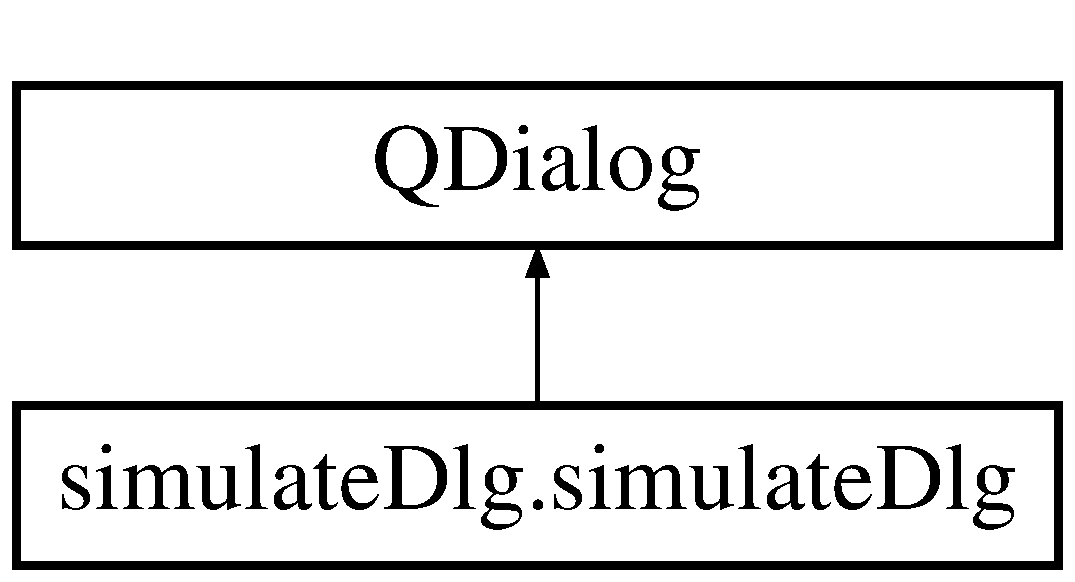
\includegraphics[height=2.000000cm]{classsimulateDlg_1_1simulateDlg}
\end{center}
\end{figure}
\subsection*{Public Member Functions}
\begin{DoxyCompactItemize}
\item 
\hypertarget{classsimulateDlg_1_1simulateDlg_a30e20ab290a85ace9b9f1aa244d7c474}{def {\bfseries \-\_\-\-\_\-init\-\_\-\-\_\-}}\label{classsimulateDlg_1_1simulateDlg_a30e20ab290a85ace9b9f1aa244d7c474}

\item 
\hypertarget{classsimulateDlg_1_1simulateDlg_ae8ad62465bea76aeb7ced4d34d8ca56a}{def {\bfseries set\-Work\-Dir}}\label{classsimulateDlg_1_1simulateDlg_ae8ad62465bea76aeb7ced4d34d8ca56a}

\item 
\hypertarget{classsimulateDlg_1_1simulateDlg_a53b3c5047a7a281b5baeec7135492591}{def {\bfseries set\-B\-Size\-Control}}\label{classsimulateDlg_1_1simulateDlg_a53b3c5047a7a281b5baeec7135492591}

\item 
\hypertarget{classsimulateDlg_1_1simulateDlg_a97123c1f3e8b1b340dc382a6fd86a101}{def {\bfseries set\-Exclude\-Control}}\label{classsimulateDlg_1_1simulateDlg_a97123c1f3e8b1b340dc382a6fd86a101}

\item 
\hypertarget{classsimulateDlg_1_1simulateDlg_abe6b4f3fef4b78d2c7a2555727653de1}{def {\bfseries set\-Detector}}\label{classsimulateDlg_1_1simulateDlg_abe6b4f3fef4b78d2c7a2555727653de1}

\item 
\hypertarget{classsimulateDlg_1_1simulateDlg_a3087ff8625ca2596757a04e8d57c6aef}{def {\bfseries set\-Peak\-Table}}\label{classsimulateDlg_1_1simulateDlg_a3087ff8625ca2596757a04e8d57c6aef}

\item 
\hypertarget{classsimulateDlg_1_1simulateDlg_ac656f0af5fb6ead3d58c3a79cbe90453}{def {\bfseries set\-Predict}}\label{classsimulateDlg_1_1simulateDlg_ac656f0af5fb6ead3d58c3a79cbe90453}

\item 
\hypertarget{classsimulateDlg_1_1simulateDlg_afc7435e2812554e7059d3d9e908183ff}{def {\bfseries set\-Project}}\label{classsimulateDlg_1_1simulateDlg_afc7435e2812554e7059d3d9e908183ff}

\item 
\hypertarget{classsimulateDlg_1_1simulateDlg_a251194e1c458621e24fdfdeb409342c6}{def {\bfseries fill\-Up}}\label{classsimulateDlg_1_1simulateDlg_a251194e1c458621e24fdfdeb409342c6}

\item 
\hypertarget{classsimulateDlg_1_1simulateDlg_a8d07b8b8fbaebf05066a368ef55d1c3e}{def {\bfseries inc\-Val}}\label{classsimulateDlg_1_1simulateDlg_a8d07b8b8fbaebf05066a368ef55d1c3e}

\item 
\hypertarget{classsimulateDlg_1_1simulateDlg_a686a9c2d3206667c4f54f742537dc0f4}{def {\bfseries dec\-Val}}\label{classsimulateDlg_1_1simulateDlg_a686a9c2d3206667c4f54f742537dc0f4}

\item 
\hypertarget{classsimulateDlg_1_1simulateDlg_ae7f76a72f48eadc2aa799a2a2a66c24f}{def {\bfseries rad\-State}}\label{classsimulateDlg_1_1simulateDlg_ae7f76a72f48eadc2aa799a2a2a66c24f}

\item 
\hypertarget{classsimulateDlg_1_1simulateDlg_a9c525e6091e98de8f7da2fa5390e7f45}{def {\bfseries gen\-B}}\label{classsimulateDlg_1_1simulateDlg_a9c525e6091e98de8f7da2fa5390e7f45}

\item 
\hypertarget{classsimulateDlg_1_1simulateDlg_a5420da8b718295dec6996e3af575d009}{def {\bfseries change\-B}}\label{classsimulateDlg_1_1simulateDlg_a5420da8b718295dec6996e3af575d009}

\item 
\hypertarget{classsimulateDlg_1_1simulateDlg_ab5bf1b8be44923ad6767d7b26e24dfba}{def {\bfseries reset\-O\-C\-P}}\label{classsimulateDlg_1_1simulateDlg_ab5bf1b8be44923ad6767d7b26e24dfba}

\item 
\hypertarget{classsimulateDlg_1_1simulateDlg_a36b13c633095fd1b37a8c24bdc9feb02}{def {\bfseries read\-\_\-\-L\-P}}\label{classsimulateDlg_1_1simulateDlg_a36b13c633095fd1b37a8c24bdc9feb02}

\item 
\hypertarget{classsimulateDlg_1_1simulateDlg_a541dcb68081dc45190cf99d019e34abb}{def {\bfseries print\-\_\-\-L\-P}}\label{classsimulateDlg_1_1simulateDlg_a541dcb68081dc45190cf99d019e34abb}

\item 
\hypertarget{classsimulateDlg_1_1simulateDlg_a670a1ff9f543741845ce493b6cd74a3c}{def \hyperlink{classsimulateDlg_1_1simulateDlg_a670a1ff9f543741845ce493b6cd74a3c}{open\-U\-B}}\label{classsimulateDlg_1_1simulateDlg_a670a1ff9f543741845ce493b6cd74a3c}

\begin{DoxyCompactList}\small\item\em open U\-B matrix \end{DoxyCompactList}\item 
\hypertarget{classsimulateDlg_1_1simulateDlg_a581c5c28fe9bf57a0de93fcb1e8859aa}{def {\bfseries load\-U\-B}}\label{classsimulateDlg_1_1simulateDlg_a581c5c28fe9bf57a0de93fcb1e8859aa}

\item 
\hypertarget{classsimulateDlg_1_1simulateDlg_af4dec6ad7208da45bb52d9d42f4d16ce}{def {\bfseries save\-U\-B}}\label{classsimulateDlg_1_1simulateDlg_af4dec6ad7208da45bb52d9d42f4d16ce}

\item 
\hypertarget{classsimulateDlg_1_1simulateDlg_ad9f8e5700a177c99d6d602a897240408}{def {\bfseries display\-Matrix}}\label{classsimulateDlg_1_1simulateDlg_ad9f8e5700a177c99d6d602a897240408}

\item 
\hypertarget{classsimulateDlg_1_1simulateDlg_aa4af2d01c58f4243d379c31a9a46f45c}{def {\bfseries assign\-H\-K\-L}}\label{classsimulateDlg_1_1simulateDlg_aa4af2d01c58f4243d379c31a9a46f45c}

\item 
\hypertarget{classsimulateDlg_1_1simulateDlg_a234c4ec7bdd66c1146e769d3e2cb757b}{def {\bfseries generate}}\label{classsimulateDlg_1_1simulateDlg_a234c4ec7bdd66c1146e769d3e2cb757b}

\item 
\hypertarget{classsimulateDlg_1_1simulateDlg_a1e8f99f0c2ba8218f61c039d7456a62a}{def {\bfseries index}}\label{classsimulateDlg_1_1simulateDlg_a1e8f99f0c2ba8218f61c039d7456a62a}

\item 
\hypertarget{classsimulateDlg_1_1simulateDlg_a5785ed6c6f50cc4276949b204b39dd62}{def {\bfseries get\-Bravais\-Type}}\label{classsimulateDlg_1_1simulateDlg_a5785ed6c6f50cc4276949b204b39dd62}

\item 
\hypertarget{classsimulateDlg_1_1simulateDlg_a6bc9d5aedaf9bf4452cb118b7a4dab01}{def {\bfseries generate\-\_\-laue}}\label{classsimulateDlg_1_1simulateDlg_a6bc9d5aedaf9bf4452cb118b7a4dab01}

\item 
\hypertarget{classsimulateDlg_1_1simulateDlg_ad93d6457999611add68e57fea7270e2a}{def {\bfseries generate\-\_\-mono}}\label{classsimulateDlg_1_1simulateDlg_ad93d6457999611add68e57fea7270e2a}

\item 
\hypertarget{classsimulateDlg_1_1simulateDlg_a2c6753d7216124538a12c8b5f8157c43}{def {\bfseries read\-\_\-box\-\_\-size}}\label{classsimulateDlg_1_1simulateDlg_a2c6753d7216124538a12c8b5f8157c43}

\item 
\hypertarget{classsimulateDlg_1_1simulateDlg_a3464acfdc69fd672f3ea82d6408fede7}{def {\bfseries close\-Up}}\label{classsimulateDlg_1_1simulateDlg_a3464acfdc69fd672f3ea82d6408fede7}

\end{DoxyCompactItemize}
\subsection*{Public Attributes}
\begin{DoxyCompactItemize}
\item 
\hypertarget{classsimulateDlg_1_1simulateDlg_a23a3d39d70f0ae6ce8a838fe680afd08}{{\bfseries ui}}\label{classsimulateDlg_1_1simulateDlg_a23a3d39d70f0ae6ce8a838fe680afd08}

\item 
\hypertarget{classsimulateDlg_1_1simulateDlg_ad2226009f457b82889ed337b1ed49e4b}{{\bfseries my\-Detect}}\label{classsimulateDlg_1_1simulateDlg_ad2226009f457b82889ed337b1ed49e4b}

\item 
\hypertarget{classsimulateDlg_1_1simulateDlg_a7ebdd328ed6aa4ac6e050c23ff4d4d50}{{\bfseries dac\-Open}}\label{classsimulateDlg_1_1simulateDlg_a7ebdd328ed6aa4ac6e050c23ff4d4d50}

\item 
\hypertarget{classsimulateDlg_1_1simulateDlg_a5aa51d22e30acd26145131e848e30759}{{\bfseries ub}}\label{classsimulateDlg_1_1simulateDlg_a5aa51d22e30acd26145131e848e30759}

\item 
\hypertarget{classsimulateDlg_1_1simulateDlg_afb873a7d23504a37dc242405343f64aa}{{\bfseries my\-Predict}}\label{classsimulateDlg_1_1simulateDlg_afb873a7d23504a37dc242405343f64aa}

\item 
\hypertarget{classsimulateDlg_1_1simulateDlg_a714be7d1a5fb648271c987444d5be3c4}{{\bfseries my\-Peaks}}\label{classsimulateDlg_1_1simulateDlg_a714be7d1a5fb648271c987444d5be3c4}

\item 
\hypertarget{classsimulateDlg_1_1simulateDlg_aed2a79b17c8c625b06bad686996395e8}{{\bfseries brav\-Type}}\label{classsimulateDlg_1_1simulateDlg_aed2a79b17c8c625b06bad686996395e8}

\item 
\hypertarget{classsimulateDlg_1_1simulateDlg_a217be5c43518b4f44ac9f9397e4cd155}{{\bfseries workdir}}\label{classsimulateDlg_1_1simulateDlg_a217be5c43518b4f44ac9f9397e4cd155}

\item 
\hypertarget{classsimulateDlg_1_1simulateDlg_a37752b91546a36f94ff8e4dedee83518}{{\bfseries base}}\label{classsimulateDlg_1_1simulateDlg_a37752b91546a36f94ff8e4dedee83518}

\item 
\hypertarget{classsimulateDlg_1_1simulateDlg_a6b8afedfdaab0461117c61cde727aa2d}{{\bfseries proj\-Flag}}\label{classsimulateDlg_1_1simulateDlg_a6b8afedfdaab0461117c61cde727aa2d}

\item 
\hypertarget{classsimulateDlg_1_1simulateDlg_a2b03e2e70fbf25c638c1e0466a2de38f}{{\bfseries bs\-Control}}\label{classsimulateDlg_1_1simulateDlg_a2b03e2e70fbf25c638c1e0466a2de38f}

\item 
\hypertarget{classsimulateDlg_1_1simulateDlg_a2adb9273893575b3120e8878a99983d4}{{\bfseries exclude\-C\-Box}}\label{classsimulateDlg_1_1simulateDlg_a2adb9273893575b3120e8878a99983d4}

\item 
\hypertarget{classsimulateDlg_1_1simulateDlg_a723b0e1c3aa3f071ae84ec39a1558845}{{\bfseries project}}\label{classsimulateDlg_1_1simulateDlg_a723b0e1c3aa3f071ae84ec39a1558845}

\end{DoxyCompactItemize}
\subsection*{Static Public Attributes}
\begin{DoxyCompactItemize}
\item 
\hypertarget{classsimulateDlg_1_1simulateDlg_a14c3146ee7422f53d8488a114344800e}{tuple {\bfseries update\-Peaks} = Qt\-Core.\-pyqt\-Signal()}\label{classsimulateDlg_1_1simulateDlg_a14c3146ee7422f53d8488a114344800e}

\item 
\hypertarget{classsimulateDlg_1_1simulateDlg_a1c6d77c7b4759cb95a7fbdd5a7ca23d7}{tuple {\bfseries update\-Display} = Qt\-Core.\-pyqt\-Signal()}\label{classsimulateDlg_1_1simulateDlg_a1c6d77c7b4759cb95a7fbdd5a7ca23d7}

\end{DoxyCompactItemize}


The documentation for this class was generated from the following file\-:\begin{DoxyCompactItemize}
\item 
/home/harold/workdir/atrex/\-Software/simulate\-Dlg.\-py\end{DoxyCompactItemize}

\hypertarget{classPrzemek__testing_1_1tester}{\section{Przemek\-\_\-testing.\-tester Class Reference}
\label{classPrzemek__testing_1_1tester}\index{Przemek\-\_\-testing.\-tester@{Przemek\-\_\-testing.\-tester}}
}
\subsection*{Static Public Attributes}
\begin{DoxyCompactItemize}
\item 
\hypertarget{classPrzemek__testing_1_1tester_a3b224f5c318c0a6ff10f84f3ed1ae172}{tuple {\bfseries a} = \hyperlink{classmyPeakTable_1_1myPeakTable}{my\-Peak\-Table.\-my\-Peak\-Table}()}\label{classPrzemek__testing_1_1tester_a3b224f5c318c0a6ff10f84f3ed1ae172}

\item 
\hypertarget{classPrzemek__testing_1_1tester_a567760c83534060e622ca5c14ba7d393}{tuple {\bfseries b} = \hyperlink{classmyPeakTable_1_1myPeakTable}{my\-Peak\-Table.\-my\-Peak\-Table}()}\label{classPrzemek__testing_1_1tester_a567760c83534060e622ca5c14ba7d393}

\end{DoxyCompactItemize}


The documentation for this class was generated from the following file\-:\begin{DoxyCompactItemize}
\item 
/home/harold/workdir/atrex/\-Software/Przemek\-\_\-testing.\-py\end{DoxyCompactItemize}

\hypertarget{classtifffile_1_1TIFF__SUBFILE__TYPES}{\section{tifffile.\-T\-I\-F\-F\-\_\-\-S\-U\-B\-F\-I\-L\-E\-\_\-\-T\-Y\-P\-E\-S Class Reference}
\label{classtifffile_1_1TIFF__SUBFILE__TYPES}\index{tifffile.\-T\-I\-F\-F\-\_\-\-S\-U\-B\-F\-I\-L\-E\-\_\-\-T\-Y\-P\-E\-S@{tifffile.\-T\-I\-F\-F\-\_\-\-S\-U\-B\-F\-I\-L\-E\-\_\-\-T\-Y\-P\-E\-S}}
}
Inheritance diagram for tifffile.\-T\-I\-F\-F\-\_\-\-S\-U\-B\-F\-I\-L\-E\-\_\-\-T\-Y\-P\-E\-S\-:\begin{figure}[H]
\begin{center}
\leavevmode
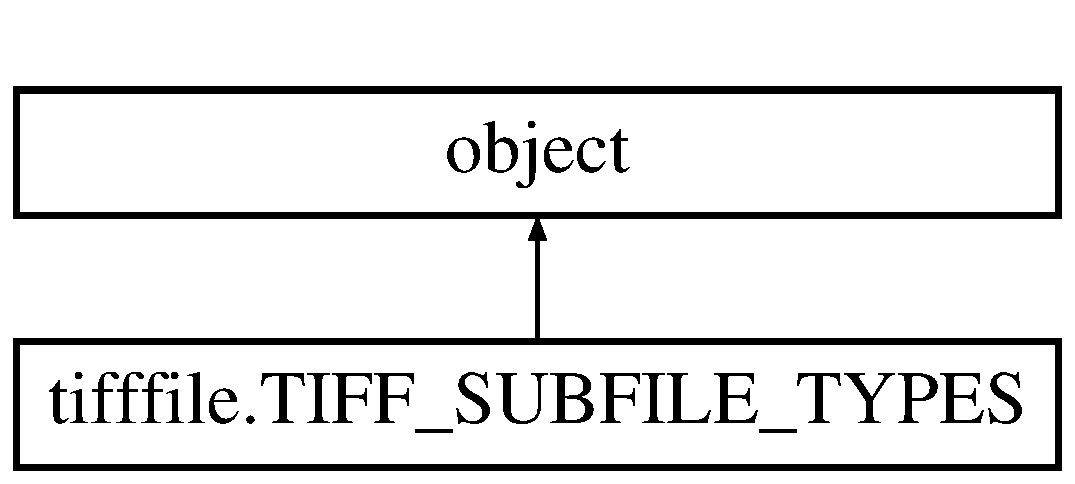
\includegraphics[height=2.000000cm]{classtifffile_1_1TIFF__SUBFILE__TYPES}
\end{center}
\end{figure}
\subsection*{Public Member Functions}
\begin{DoxyCompactItemize}
\item 
\hypertarget{classtifffile_1_1TIFF__SUBFILE__TYPES_a64c992e0cabb37664338e4a7edfa34c8}{def {\bfseries \-\_\-\-\_\-getitem\-\_\-\-\_\-}}\label{classtifffile_1_1TIFF__SUBFILE__TYPES_a64c992e0cabb37664338e4a7edfa34c8}

\end{DoxyCompactItemize}


The documentation for this class was generated from the following file\-:\begin{DoxyCompactItemize}
\item 
/home/harold/workdir/atrex/\-Software/tifffile.\-py\end{DoxyCompactItemize}

\hypertarget{classtifffile_1_1TiffFile}{\section{tifffile.\-Tiff\-File Class Reference}
\label{classtifffile_1_1TiffFile}\index{tifffile.\-Tiff\-File@{tifffile.\-Tiff\-File}}
}
Inheritance diagram for tifffile.\-Tiff\-File\-:\begin{figure}[H]
\begin{center}
\leavevmode
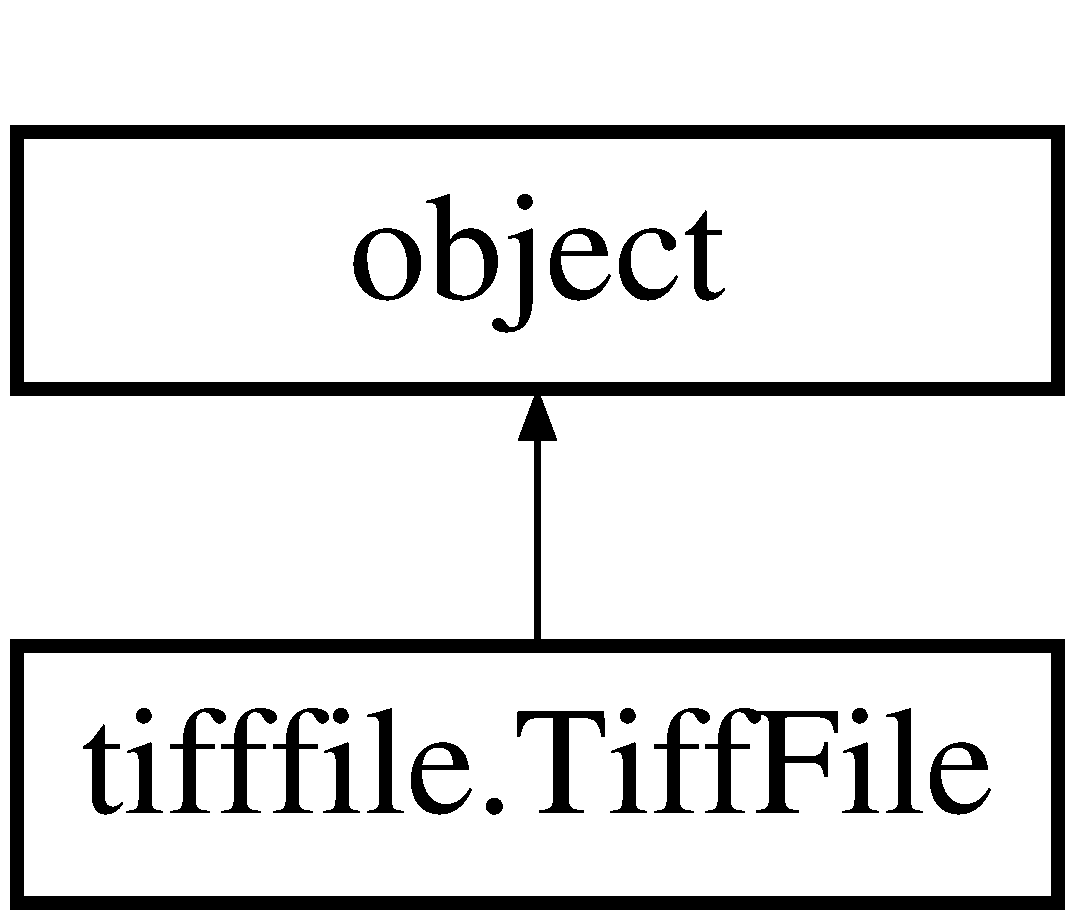
\includegraphics[height=2.000000cm]{classtifffile_1_1TiffFile}
\end{center}
\end{figure}
\subsection*{Public Member Functions}
\begin{DoxyCompactItemize}
\item 
def \hyperlink{classtifffile_1_1TiffFile_a2cacc91d936a85b866629e1004db56be}{\-\_\-\-\_\-init\-\_\-\-\_\-}
\item 
def \hyperlink{classtifffile_1_1TiffFile_ab60b7755da796bc24e0959901a2178f2}{filehandle}
\item 
def \hyperlink{classtifffile_1_1TiffFile_a6215683006e55ed5602df52a5596b6c2}{filename}
\item 
def \hyperlink{classtifffile_1_1TiffFile_aeee11d1813bfd5ca6684468bb771f214}{close}
\item 
def \hyperlink{classtifffile_1_1TiffFile_a774e670bd07b1bfc5f06ccd52a6a800a}{series}
\item 
def \hyperlink{classtifffile_1_1TiffFile_a6ffb819278ba899e42fd6253508bcb8a}{asarray}
\item 
def \hyperlink{classtifffile_1_1TiffFile_a9e400571d3475d5e268893877136bf24}{\-\_\-\-\_\-len\-\_\-\-\_\-}
\item 
def \hyperlink{classtifffile_1_1TiffFile_addf7084c3ea60f31fa8f19b4db5284a4}{\-\_\-\-\_\-getitem\-\_\-\-\_\-}
\item 
def \hyperlink{classtifffile_1_1TiffFile_a12847e8b06cb8c2c4b9233377eaec539}{\-\_\-\-\_\-iter\-\_\-\-\_\-}
\item 
def \hyperlink{classtifffile_1_1TiffFile_a090018b858ceac412aafeae6c6c29a89}{\-\_\-\-\_\-str\-\_\-\-\_\-}
\item 
\hypertarget{classtifffile_1_1TiffFile_a8af0d38a6308893259f009a848dc8f55}{def {\bfseries \-\_\-\-\_\-enter\-\_\-\-\_\-}}\label{classtifffile_1_1TiffFile_a8af0d38a6308893259f009a848dc8f55}

\item 
\hypertarget{classtifffile_1_1TiffFile_a86dacb85206d356ff3da93bec1ed0848}{def {\bfseries \-\_\-\-\_\-exit\-\_\-\-\_\-}}\label{classtifffile_1_1TiffFile_a86dacb85206d356ff3da93bec1ed0848}

\item 
\hypertarget{classtifffile_1_1TiffFile_a930a149ecaf1ad9409c4dbad1d9c2d60}{def {\bfseries fstat}}\label{classtifffile_1_1TiffFile_a930a149ecaf1ad9409c4dbad1d9c2d60}

\item 
\hypertarget{classtifffile_1_1TiffFile_af5d955e517896fee54d9fe3d9e9f266c}{def {\bfseries is\-\_\-bigtiff}}\label{classtifffile_1_1TiffFile_af5d955e517896fee54d9fe3d9e9f266c}

\item 
\hypertarget{classtifffile_1_1TiffFile_a633ef6274a2c54e1af3f1e01c9e6ee66}{def {\bfseries is\-\_\-rgb}}\label{classtifffile_1_1TiffFile_a633ef6274a2c54e1af3f1e01c9e6ee66}

\item 
\hypertarget{classtifffile_1_1TiffFile_a610addce1bfe1fe31aed918f358bdeaf}{def {\bfseries is\-\_\-palette}}\label{classtifffile_1_1TiffFile_a610addce1bfe1fe31aed918f358bdeaf}

\item 
\hypertarget{classtifffile_1_1TiffFile_a48749abc5c5eaf5e11cd731104c22cb9}{def {\bfseries is\-\_\-mdgel}}\label{classtifffile_1_1TiffFile_a48749abc5c5eaf5e11cd731104c22cb9}

\item 
\hypertarget{classtifffile_1_1TiffFile_a491c0c01ccff753773477ff0adc2b1c3}{def {\bfseries is\-\_\-mediacy}}\label{classtifffile_1_1TiffFile_a491c0c01ccff753773477ff0adc2b1c3}

\item 
\hypertarget{classtifffile_1_1TiffFile_a3aef6d37c74dc3c2ae8d319f1680e4cd}{def {\bfseries is\-\_\-stk}}\label{classtifffile_1_1TiffFile_a3aef6d37c74dc3c2ae8d319f1680e4cd}

\item 
\hypertarget{classtifffile_1_1TiffFile_a4b62231ac45a69f35b4eebe2cafd9233}{def {\bfseries is\-\_\-lsm}}\label{classtifffile_1_1TiffFile_a4b62231ac45a69f35b4eebe2cafd9233}

\item 
\hypertarget{classtifffile_1_1TiffFile_a57ccede80811571fa599f67771f35c6a}{def {\bfseries is\-\_\-imagej}}\label{classtifffile_1_1TiffFile_a57ccede80811571fa599f67771f35c6a}

\item 
\hypertarget{classtifffile_1_1TiffFile_a3ae5c2e4f211833e4d830c1af04b9b9f}{def {\bfseries is\-\_\-micromanager}}\label{classtifffile_1_1TiffFile_a3ae5c2e4f211833e4d830c1af04b9b9f}

\item 
\hypertarget{classtifffile_1_1TiffFile_a4b98fd0ade83b2679ecd2da1230196a1}{def {\bfseries is\-\_\-nih}}\label{classtifffile_1_1TiffFile_a4b98fd0ade83b2679ecd2da1230196a1}

\item 
\hypertarget{classtifffile_1_1TiffFile_a1f6562d875ce250d67b1566aaf49d9f7}{def {\bfseries is\-\_\-fluoview}}\label{classtifffile_1_1TiffFile_a1f6562d875ce250d67b1566aaf49d9f7}

\item 
\hypertarget{classtifffile_1_1TiffFile_acab85c4f4398924ad3cc041ef4beee90}{def {\bfseries is\-\_\-ome}}\label{classtifffile_1_1TiffFile_acab85c4f4398924ad3cc041ef4beee90}

\end{DoxyCompactItemize}
\subsection*{Public Attributes}
\begin{DoxyCompactItemize}
\item 
\hypertarget{classtifffile_1_1TiffFile_ab531ab5699a9b426c32e26444e8e53ac}{{\bfseries offset\-\_\-size}}\label{classtifffile_1_1TiffFile_ab531ab5699a9b426c32e26444e8e53ac}

\item 
\hypertarget{classtifffile_1_1TiffFile_a38687a2ea2711cef070cf0b9ddb4e65f}{{\bfseries pages}}\label{classtifffile_1_1TiffFile_a38687a2ea2711cef070cf0b9ddb4e65f}

\item 
\hypertarget{classtifffile_1_1TiffFile_a9482f0d20fef11df3b9baaa04f8a7bb6}{{\bfseries byteorder}}\label{classtifffile_1_1TiffFile_a9482f0d20fef11df3b9baaa04f8a7bb6}

\item 
\hypertarget{classtifffile_1_1TiffFile_ad38661d0b0a16180347517d5ff208afd}{{\bfseries micromanager\-\_\-metadata}}\label{classtifffile_1_1TiffFile_ad38661d0b0a16180347517d5ff208afd}

\item 
\hypertarget{classtifffile_1_1TiffFile_acc082b0de522251b75669336fe57b005}{{\bfseries master}}\label{classtifffile_1_1TiffFile_acc082b0de522251b75669336fe57b005}

\item 
\hypertarget{classtifffile_1_1TiffFile_a29b8b6eb049a61de92b16223f75492e0}{{\bfseries parent}}\label{classtifffile_1_1TiffFile_a29b8b6eb049a61de92b16223f75492e0}

\end{DoxyCompactItemize}


\subsection{Detailed Description}
\begin{DoxyVerb}Read image and metadata from TIFF, STK, LSM, and FluoView files.

TiffFile instances must be closed using the close method, which is
automatically called when using the 'with' statement.

Attributes
----------
pages : list
    All TIFF pages in file.
series : list of Records(shape, dtype, axes, TiffPages)
    TIFF pages with compatible shapes and types.
micromanager_metadata: dict
    Extra MicroManager non-TIFF metadata in the file, if exists.

All attributes are read-only.

Examples
--------
>>> with TiffFile('test.tif') as tif:
...     data = tif.asarray()
...     data.shape
(256, 256, 4)\end{DoxyVerb}
 

\subsection{Constructor \& Destructor Documentation}
\hypertarget{classtifffile_1_1TiffFile_a2cacc91d936a85b866629e1004db56be}{\index{tifffile\-::\-Tiff\-File@{tifffile\-::\-Tiff\-File}!\-\_\-\-\_\-init\-\_\-\-\_\-@{\-\_\-\-\_\-init\-\_\-\-\_\-}}
\index{\-\_\-\-\_\-init\-\_\-\-\_\-@{\-\_\-\-\_\-init\-\_\-\-\_\-}!tifffile::TiffFile@{tifffile\-::\-Tiff\-File}}
\subsubsection[{\-\_\-\-\_\-init\-\_\-\-\_\-}]{\setlength{\rightskip}{0pt plus 5cm}def tifffile.\-Tiff\-File.\-\_\-\-\_\-init\-\_\-\-\_\- (
\begin{DoxyParamCaption}
\item[{}]{self, }
\item[{}]{arg, }
\item[{}]{name = {\ttfamily None}, }
\item[{}]{offset = {\ttfamily None}, }
\item[{}]{size = {\ttfamily None}, }
\item[{}]{multifile = {\ttfamily True}, }
\item[{}]{multifile\-\_\-close = {\ttfamily True}}
\end{DoxyParamCaption}
)}}\label{classtifffile_1_1TiffFile_a2cacc91d936a85b866629e1004db56be}
\begin{DoxyVerb}Initialize instance from file.

Parameters
----------
arg : str or open file
    Name of file or open file object.
    The file objects are closed in TiffFile.close().
name : str
    Optional name of file in case 'arg' is a file handle.
offset : int
    Optional start position of embedded file. By default this is
    the current file position.
size : int
    Optional size of embedded file. By default this is the number
    of bytes from the 'offset' to the end of the file.
multifile : bool
    If True (default), series may include pages from multiple files.
    Currently applies to OME-TIFF only.
multifile_close : bool
    If True (default), keep the handles of other files in multifile
    series closed. This is inefficient when few files refer to
    many pages. If False, the C runtime may run out of resources.\end{DoxyVerb}
 

\subsection{Member Function Documentation}
\hypertarget{classtifffile_1_1TiffFile_addf7084c3ea60f31fa8f19b4db5284a4}{\index{tifffile\-::\-Tiff\-File@{tifffile\-::\-Tiff\-File}!\-\_\-\-\_\-getitem\-\_\-\-\_\-@{\-\_\-\-\_\-getitem\-\_\-\-\_\-}}
\index{\-\_\-\-\_\-getitem\-\_\-\-\_\-@{\-\_\-\-\_\-getitem\-\_\-\-\_\-}!tifffile::TiffFile@{tifffile\-::\-Tiff\-File}}
\subsubsection[{\-\_\-\-\_\-getitem\-\_\-\-\_\-}]{\setlength{\rightskip}{0pt plus 5cm}def tifffile.\-Tiff\-File.\-\_\-\-\_\-getitem\-\_\-\-\_\- (
\begin{DoxyParamCaption}
\item[{}]{self, }
\item[{}]{key}
\end{DoxyParamCaption}
)}}\label{classtifffile_1_1TiffFile_addf7084c3ea60f31fa8f19b4db5284a4}
\begin{DoxyVerb}Return specified page.\end{DoxyVerb}
 \hypertarget{classtifffile_1_1TiffFile_a12847e8b06cb8c2c4b9233377eaec539}{\index{tifffile\-::\-Tiff\-File@{tifffile\-::\-Tiff\-File}!\-\_\-\-\_\-iter\-\_\-\-\_\-@{\-\_\-\-\_\-iter\-\_\-\-\_\-}}
\index{\-\_\-\-\_\-iter\-\_\-\-\_\-@{\-\_\-\-\_\-iter\-\_\-\-\_\-}!tifffile::TiffFile@{tifffile\-::\-Tiff\-File}}
\subsubsection[{\-\_\-\-\_\-iter\-\_\-\-\_\-}]{\setlength{\rightskip}{0pt plus 5cm}def tifffile.\-Tiff\-File.\-\_\-\-\_\-iter\-\_\-\-\_\- (
\begin{DoxyParamCaption}
\item[{}]{self}
\end{DoxyParamCaption}
)}}\label{classtifffile_1_1TiffFile_a12847e8b06cb8c2c4b9233377eaec539}
\begin{DoxyVerb}Return iterator over pages.\end{DoxyVerb}
 \hypertarget{classtifffile_1_1TiffFile_a9e400571d3475d5e268893877136bf24}{\index{tifffile\-::\-Tiff\-File@{tifffile\-::\-Tiff\-File}!\-\_\-\-\_\-len\-\_\-\-\_\-@{\-\_\-\-\_\-len\-\_\-\-\_\-}}
\index{\-\_\-\-\_\-len\-\_\-\-\_\-@{\-\_\-\-\_\-len\-\_\-\-\_\-}!tifffile::TiffFile@{tifffile\-::\-Tiff\-File}}
\subsubsection[{\-\_\-\-\_\-len\-\_\-\-\_\-}]{\setlength{\rightskip}{0pt plus 5cm}def tifffile.\-Tiff\-File.\-\_\-\-\_\-len\-\_\-\-\_\- (
\begin{DoxyParamCaption}
\item[{}]{self}
\end{DoxyParamCaption}
)}}\label{classtifffile_1_1TiffFile_a9e400571d3475d5e268893877136bf24}
\begin{DoxyVerb}Return number of image pages in file.\end{DoxyVerb}
 \hypertarget{classtifffile_1_1TiffFile_a090018b858ceac412aafeae6c6c29a89}{\index{tifffile\-::\-Tiff\-File@{tifffile\-::\-Tiff\-File}!\-\_\-\-\_\-str\-\_\-\-\_\-@{\-\_\-\-\_\-str\-\_\-\-\_\-}}
\index{\-\_\-\-\_\-str\-\_\-\-\_\-@{\-\_\-\-\_\-str\-\_\-\-\_\-}!tifffile::TiffFile@{tifffile\-::\-Tiff\-File}}
\subsubsection[{\-\_\-\-\_\-str\-\_\-\-\_\-}]{\setlength{\rightskip}{0pt plus 5cm}def tifffile.\-Tiff\-File.\-\_\-\-\_\-str\-\_\-\-\_\- (
\begin{DoxyParamCaption}
\item[{}]{self}
\end{DoxyParamCaption}
)}}\label{classtifffile_1_1TiffFile_a090018b858ceac412aafeae6c6c29a89}
\begin{DoxyVerb}Return string containing information about file.\end{DoxyVerb}
 \hypertarget{classtifffile_1_1TiffFile_a6ffb819278ba899e42fd6253508bcb8a}{\index{tifffile\-::\-Tiff\-File@{tifffile\-::\-Tiff\-File}!asarray@{asarray}}
\index{asarray@{asarray}!tifffile::TiffFile@{tifffile\-::\-Tiff\-File}}
\subsubsection[{asarray}]{\setlength{\rightskip}{0pt plus 5cm}def tifffile.\-Tiff\-File.\-asarray (
\begin{DoxyParamCaption}
\item[{}]{self, }
\item[{}]{key = {\ttfamily None}, }
\item[{}]{series = {\ttfamily None}, }
\item[{}]{memmap = {\ttfamily False}}
\end{DoxyParamCaption}
)}}\label{classtifffile_1_1TiffFile_a6ffb819278ba899e42fd6253508bcb8a}
\begin{DoxyVerb}Return image data from multiple TIFF pages as numpy array.

By default the first image series is returned.

Parameters
----------
key : int, slice, or sequence of page indices
    Defines which pages to return as array.
series : int
    Defines which series of pages to return as array.
memmap : bool
    If True, return an array stored in a binary file on disk
    if possible.\end{DoxyVerb}
 \hypertarget{classtifffile_1_1TiffFile_aeee11d1813bfd5ca6684468bb771f214}{\index{tifffile\-::\-Tiff\-File@{tifffile\-::\-Tiff\-File}!close@{close}}
\index{close@{close}!tifffile::TiffFile@{tifffile\-::\-Tiff\-File}}
\subsubsection[{close}]{\setlength{\rightskip}{0pt plus 5cm}def tifffile.\-Tiff\-File.\-close (
\begin{DoxyParamCaption}
\item[{}]{self}
\end{DoxyParamCaption}
)}}\label{classtifffile_1_1TiffFile_aeee11d1813bfd5ca6684468bb771f214}
\begin{DoxyVerb}Close open file handle(s).\end{DoxyVerb}
 \hypertarget{classtifffile_1_1TiffFile_ab60b7755da796bc24e0959901a2178f2}{\index{tifffile\-::\-Tiff\-File@{tifffile\-::\-Tiff\-File}!filehandle@{filehandle}}
\index{filehandle@{filehandle}!tifffile::TiffFile@{tifffile\-::\-Tiff\-File}}
\subsubsection[{filehandle}]{\setlength{\rightskip}{0pt plus 5cm}def tifffile.\-Tiff\-File.\-filehandle (
\begin{DoxyParamCaption}
\item[{}]{self}
\end{DoxyParamCaption}
)}}\label{classtifffile_1_1TiffFile_ab60b7755da796bc24e0959901a2178f2}
\begin{DoxyVerb}Return file handle.\end{DoxyVerb}
 \hypertarget{classtifffile_1_1TiffFile_a6215683006e55ed5602df52a5596b6c2}{\index{tifffile\-::\-Tiff\-File@{tifffile\-::\-Tiff\-File}!filename@{filename}}
\index{filename@{filename}!tifffile::TiffFile@{tifffile\-::\-Tiff\-File}}
\subsubsection[{filename}]{\setlength{\rightskip}{0pt plus 5cm}def tifffile.\-Tiff\-File.\-filename (
\begin{DoxyParamCaption}
\item[{}]{self}
\end{DoxyParamCaption}
)}}\label{classtifffile_1_1TiffFile_a6215683006e55ed5602df52a5596b6c2}
\begin{DoxyVerb}Return name of file handle.\end{DoxyVerb}
 \hypertarget{classtifffile_1_1TiffFile_a774e670bd07b1bfc5f06ccd52a6a800a}{\index{tifffile\-::\-Tiff\-File@{tifffile\-::\-Tiff\-File}!series@{series}}
\index{series@{series}!tifffile::TiffFile@{tifffile\-::\-Tiff\-File}}
\subsubsection[{series}]{\setlength{\rightskip}{0pt plus 5cm}def tifffile.\-Tiff\-File.\-series (
\begin{DoxyParamCaption}
\item[{}]{self}
\end{DoxyParamCaption}
)}}\label{classtifffile_1_1TiffFile_a774e670bd07b1bfc5f06ccd52a6a800a}
\begin{DoxyVerb}Return series of TiffPage with compatible shape and properties.\end{DoxyVerb}
 

The documentation for this class was generated from the following file\-:\begin{DoxyCompactItemize}
\item 
/home/harold/workdir/atrex/\-Software/tifffile.\-py\end{DoxyCompactItemize}

\hypertarget{classtifffile_1_1TiffPage}{\section{tifffile.\-Tiff\-Page Class Reference}
\label{classtifffile_1_1TiffPage}\index{tifffile.\-Tiff\-Page@{tifffile.\-Tiff\-Page}}
}
Inheritance diagram for tifffile.\-Tiff\-Page\-:\begin{figure}[H]
\begin{center}
\leavevmode
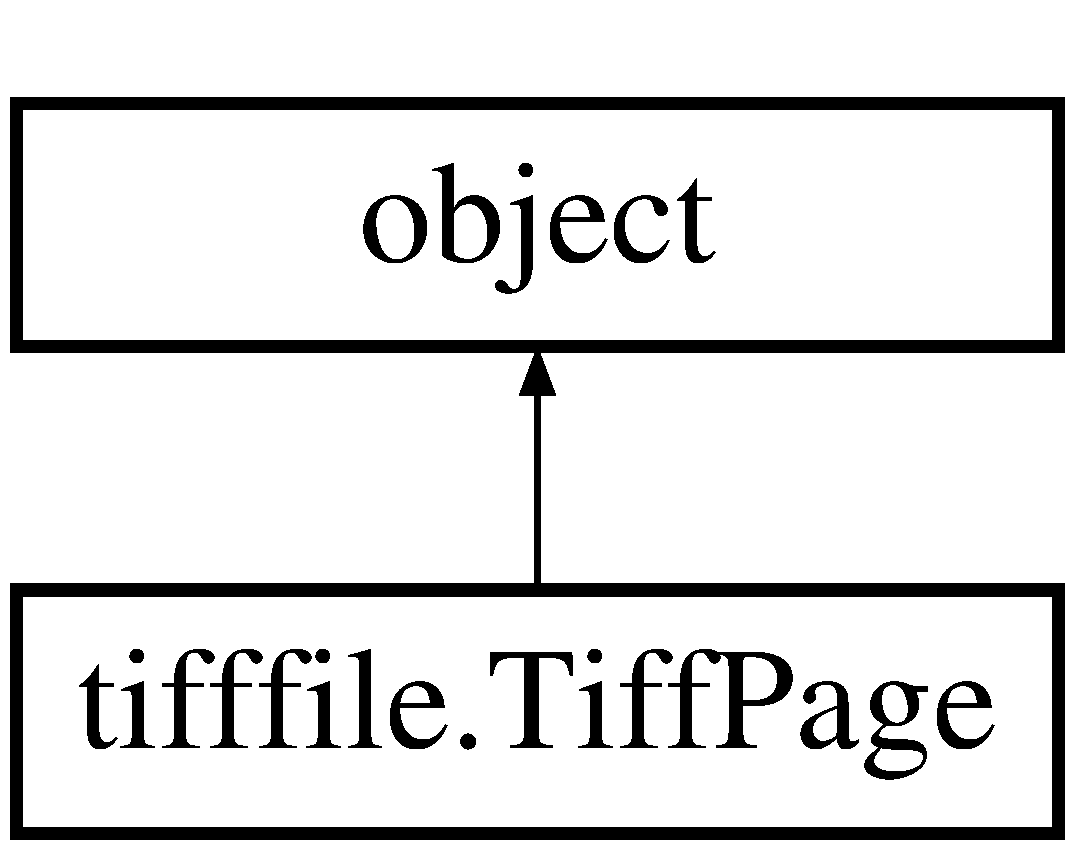
\includegraphics[height=2.000000cm]{classtifffile_1_1TiffPage}
\end{center}
\end{figure}
\subsection*{Public Member Functions}
\begin{DoxyCompactItemize}
\item 
def \hyperlink{classtifffile_1_1TiffPage_a91ce69df8f42151984d02d4054908c13}{\-\_\-\-\_\-init\-\_\-\-\_\-}
\item 
def \hyperlink{classtifffile_1_1TiffPage_a5953a258881256d704bd3d0c34a09bea}{asarray}
\item 
def \hyperlink{classtifffile_1_1TiffPage_ad0679ea4c15ca29548ae87e4986a7811}{is\-\_\-contiguous}
\item 
def \hyperlink{classtifffile_1_1TiffPage_af0e5e72edfa67d9f1239b194cbd7a56b}{\-\_\-\-\_\-str\-\_\-\-\_\-}
\item 
def \hyperlink{classtifffile_1_1TiffPage_a43cd8883f12805d887c2994582110e42}{\-\_\-\-\_\-getattr\-\_\-\-\_\-}
\item 
def \hyperlink{classtifffile_1_1TiffPage_a56fb86bb7966d84b7b72d1edc297eaed}{uic\-\_\-tags}
\item 
def \hyperlink{classtifffile_1_1TiffPage_acd582c08af3fc15fa22bbc4f6b7d4a4d}{imagej\-\_\-tags}
\item 
def \hyperlink{classtifffile_1_1TiffPage_aad80ffe0eb6611da60f78ad2743298a0}{is\-\_\-rgb}
\item 
def \hyperlink{classtifffile_1_1TiffPage_a1af194b01da49777e8d7585a987f6ccf}{is\-\_\-contig}
\item 
def \hyperlink{classtifffile_1_1TiffPage_aca723b525070789164837eb2ce3b366f}{is\-\_\-palette}
\item 
def \hyperlink{classtifffile_1_1TiffPage_afcf12e643a6207d0a02184ab19485489}{is\-\_\-tiled}
\item 
def \hyperlink{classtifffile_1_1TiffPage_af5f9892583d02082fd1be22ebe653a28}{is\-\_\-reduced}
\item 
def \hyperlink{classtifffile_1_1TiffPage_a11f2d006bbe32f212252c65a9bb9adcb}{is\-\_\-mdgel}
\item 
def \hyperlink{classtifffile_1_1TiffPage_a664758db65e7865792cc53dd01946054}{is\-\_\-mediacy}
\item 
def \hyperlink{classtifffile_1_1TiffPage_a7e17dfd14c887008863f4f800e701df1}{is\-\_\-stk}
\item 
def \hyperlink{classtifffile_1_1TiffPage_a22c271c0c693e40335409c006dc6fb0b}{is\-\_\-lsm}
\item 
def \hyperlink{classtifffile_1_1TiffPage_ab0fab509161b423ac295e4e9b1944c86}{is\-\_\-fluoview}
\item 
def \hyperlink{classtifffile_1_1TiffPage_acb4272f79554d1ca0095eb632b7a6f3b}{is\-\_\-nih}
\item 
def \hyperlink{classtifffile_1_1TiffPage_a107d6251fcd55df6f56ce4defeeb708d}{is\-\_\-sgi}
\item 
def \hyperlink{classtifffile_1_1TiffPage_a38427d4854f650021214d82f25618b98}{is\-\_\-ome}
\item 
def \hyperlink{classtifffile_1_1TiffPage_a81ea5ec5d4571a149c7217b20582873f}{is\-\_\-shaped}
\item 
def \hyperlink{classtifffile_1_1TiffPage_ada0d8196ba5f814cd827021a7cee5d1f}{is\-\_\-imagej}
\item 
def \hyperlink{classtifffile_1_1TiffPage_a792d201ffbca69b7324ecb654f0faed2}{is\-\_\-micromanager}
\end{DoxyCompactItemize}
\subsection*{Public Attributes}
\begin{DoxyCompactItemize}
\item 
\hypertarget{classtifffile_1_1TiffPage_ab448d691bfba9af88ba2658afc1b8607}{{\bfseries parent}}\label{classtifffile_1_1TiffPage_ab448d691bfba9af88ba2658afc1b8607}

\item 
\hypertarget{classtifffile_1_1TiffPage_abcdadcc105890e623a2ce56877d74c6d}{{\bfseries index}}\label{classtifffile_1_1TiffPage_abcdadcc105890e623a2ce56877d74c6d}

\item 
\hypertarget{classtifffile_1_1TiffPage_af842924ca07e0f250d2ffdcbbf1afee1}{{\bfseries shape}}\label{classtifffile_1_1TiffPage_af842924ca07e0f250d2ffdcbbf1afee1}

\item 
\hypertarget{classtifffile_1_1TiffPage_ad49c26fc7bb2cfa901aa5664879bee65}{{\bfseries dtype}}\label{classtifffile_1_1TiffPage_ad49c26fc7bb2cfa901aa5664879bee65}

\item 
\hypertarget{classtifffile_1_1TiffPage_ac28c18fcf1ee6655eaaaf035a34c9d67}{{\bfseries axes}}\label{classtifffile_1_1TiffPage_ac28c18fcf1ee6655eaaaf035a34c9d67}

\item 
\hypertarget{classtifffile_1_1TiffPage_aa35f477474445140346421065a4c016b}{{\bfseries tags}}\label{classtifffile_1_1TiffPage_aa35f477474445140346421065a4c016b}

\item 
\hypertarget{classtifffile_1_1TiffPage_a04d82b99a53cb0b445162c2e5138d136}{{\bfseries bits\-\_\-per\-\_\-sample}}\label{classtifffile_1_1TiffPage_a04d82b99a53cb0b445162c2e5138d136}

\item 
\hypertarget{classtifffile_1_1TiffPage_aef04ecb2f6f230925aeb43ac3b89e30d}{{\bfseries sample\-\_\-format}}\label{classtifffile_1_1TiffPage_aef04ecb2f6f230925aeb43ac3b89e30d}

\item 
\hypertarget{classtifffile_1_1TiffPage_af115186598b38bc4390942115755f7b6}{{\bfseries photometric}}\label{classtifffile_1_1TiffPage_af115186598b38bc4390942115755f7b6}

\item 
\hypertarget{classtifffile_1_1TiffPage_ac119ed52ce81ef4997ada9444c39562e}{{\bfseries image\-\_\-depth}}\label{classtifffile_1_1TiffPage_ac119ed52ce81ef4997ada9444c39562e}

\item 
\hypertarget{classtifffile_1_1TiffPage_a2c728cfc9795dc4bf187308d551cecb1}{{\bfseries strips\-\_\-per\-\_\-image}}\label{classtifffile_1_1TiffPage_a2c728cfc9795dc4bf187308d551cecb1}

\item 
\hypertarget{classtifffile_1_1TiffPage_aa98d8b1ccceb95ebd19896249f9f4796}{{\bfseries image\-\_\-length}}\label{classtifffile_1_1TiffPage_aa98d8b1ccceb95ebd19896249f9f4796}

\item 
\hypertarget{classtifffile_1_1TiffPage_aa16948ea525cd29705c896e1451290fa}{{\bfseries image\-\_\-width}}\label{classtifffile_1_1TiffPage_aa16948ea525cd29705c896e1451290fa}

\item 
\hypertarget{classtifffile_1_1TiffPage_aa3c254120ad8e9394ecb5c743ebf7434}{{\bfseries strip\-\_\-offsets}}\label{classtifffile_1_1TiffPage_aa3c254120ad8e9394ecb5c743ebf7434}

\item 
\hypertarget{classtifffile_1_1TiffPage_a58f5c25b8b86eb6c9a5b393e9d43c2f4}{{\bfseries color\-\_\-map}}\label{classtifffile_1_1TiffPage_a58f5c25b8b86eb6c9a5b393e9d43c2f4}

\item 
\hypertarget{classtifffile_1_1TiffPage_a376e981b0117a1be89cf336c317fd6cd}{{\bfseries is\-\_\-palette}}\label{classtifffile_1_1TiffPage_a376e981b0117a1be89cf336c317fd6cd}

\item 
\hypertarget{classtifffile_1_1TiffPage_ac55af94dba8786edaf1e89d205aed908}{{\bfseries strip\-\_\-byte\-\_\-counts}}\label{classtifffile_1_1TiffPage_ac55af94dba8786edaf1e89d205aed908}

\item 
\hypertarget{classtifffile_1_1TiffPage_af35a60f003687668b066628dc8a1c1b5}{{\bfseries compression}}\label{classtifffile_1_1TiffPage_af35a60f003687668b066628dc8a1c1b5}

\item 
\hypertarget{classtifffile_1_1TiffPage_ad51af99f663803ce6f02e124bb2db690}{{\bfseries predictor}}\label{classtifffile_1_1TiffPage_ad51af99f663803ce6f02e124bb2db690}

\end{DoxyCompactItemize}


\subsection{Detailed Description}
\begin{DoxyVerb}A TIFF image file directory (IFD).

Attributes
----------
index : int
    Index of page in file.
dtype : str {TIFF_SAMPLE_DTYPES}
    Data type of image, colormapped if applicable.
shape : tuple
    Dimensions of the image array in TIFF page,
    colormapped and with one alpha channel if applicable.
axes : str
    Axes label codes:
    'X' width, 'Y' height, 'S' sample, 'I' image series|page|plane,
    'Z' depth, 'C' color|em-wavelength|channel, 'E' ex-wavelength|lambda,
    'T' time, 'R' region|tile, 'A' angle, 'P' phase, 'H' lifetime,
    'L' exposure, 'V' event, 'Q' unknown, '_' missing
tags : TiffTags
    Dictionary of tags in page.
    Tag values are also directly accessible as attributes.
color_map : numpy array
    Color look up table, if exists.
cz_lsm_scan_info: Record(dict)
    LSM scan info attributes, if exists.
imagej_tags: Record(dict)
    Consolidated ImageJ description and metadata tags, if exists.
uic_tags: Record(dict)
    Consolidated MetaMorph STK/UIC tags, if exists.

All attributes are read-only.

Notes
-----
The internal, normalized '_shape' attribute is 6 dimensional:

0. number planes  (stk)
1. planar samples_per_pixel
2. image_depth Z  (sgi)
3. image_length Y
4. image_width X
5. contig samples_per_pixel\end{DoxyVerb}
 

\subsection{Constructor \& Destructor Documentation}
\hypertarget{classtifffile_1_1TiffPage_a91ce69df8f42151984d02d4054908c13}{\index{tifffile\-::\-Tiff\-Page@{tifffile\-::\-Tiff\-Page}!\-\_\-\-\_\-init\-\_\-\-\_\-@{\-\_\-\-\_\-init\-\_\-\-\_\-}}
\index{\-\_\-\-\_\-init\-\_\-\-\_\-@{\-\_\-\-\_\-init\-\_\-\-\_\-}!tifffile::TiffPage@{tifffile\-::\-Tiff\-Page}}
\subsubsection[{\-\_\-\-\_\-init\-\_\-\-\_\-}]{\setlength{\rightskip}{0pt plus 5cm}def tifffile.\-Tiff\-Page.\-\_\-\-\_\-init\-\_\-\-\_\- (
\begin{DoxyParamCaption}
\item[{}]{self, }
\item[{}]{parent}
\end{DoxyParamCaption}
)}}\label{classtifffile_1_1TiffPage_a91ce69df8f42151984d02d4054908c13}
\begin{DoxyVerb}Initialize instance from file.\end{DoxyVerb}
 

\subsection{Member Function Documentation}
\hypertarget{classtifffile_1_1TiffPage_a43cd8883f12805d887c2994582110e42}{\index{tifffile\-::\-Tiff\-Page@{tifffile\-::\-Tiff\-Page}!\-\_\-\-\_\-getattr\-\_\-\-\_\-@{\-\_\-\-\_\-getattr\-\_\-\-\_\-}}
\index{\-\_\-\-\_\-getattr\-\_\-\-\_\-@{\-\_\-\-\_\-getattr\-\_\-\-\_\-}!tifffile::TiffPage@{tifffile\-::\-Tiff\-Page}}
\subsubsection[{\-\_\-\-\_\-getattr\-\_\-\-\_\-}]{\setlength{\rightskip}{0pt plus 5cm}def tifffile.\-Tiff\-Page.\-\_\-\-\_\-getattr\-\_\-\-\_\- (
\begin{DoxyParamCaption}
\item[{}]{self, }
\item[{}]{name}
\end{DoxyParamCaption}
)}}\label{classtifffile_1_1TiffPage_a43cd8883f12805d887c2994582110e42}
\begin{DoxyVerb}Return tag value.\end{DoxyVerb}
 \hypertarget{classtifffile_1_1TiffPage_af0e5e72edfa67d9f1239b194cbd7a56b}{\index{tifffile\-::\-Tiff\-Page@{tifffile\-::\-Tiff\-Page}!\-\_\-\-\_\-str\-\_\-\-\_\-@{\-\_\-\-\_\-str\-\_\-\-\_\-}}
\index{\-\_\-\-\_\-str\-\_\-\-\_\-@{\-\_\-\-\_\-str\-\_\-\-\_\-}!tifffile::TiffPage@{tifffile\-::\-Tiff\-Page}}
\subsubsection[{\-\_\-\-\_\-str\-\_\-\-\_\-}]{\setlength{\rightskip}{0pt plus 5cm}def tifffile.\-Tiff\-Page.\-\_\-\-\_\-str\-\_\-\-\_\- (
\begin{DoxyParamCaption}
\item[{}]{self}
\end{DoxyParamCaption}
)}}\label{classtifffile_1_1TiffPage_af0e5e72edfa67d9f1239b194cbd7a56b}
\begin{DoxyVerb}Return string containing information about page.\end{DoxyVerb}
 \hypertarget{classtifffile_1_1TiffPage_a5953a258881256d704bd3d0c34a09bea}{\index{tifffile\-::\-Tiff\-Page@{tifffile\-::\-Tiff\-Page}!asarray@{asarray}}
\index{asarray@{asarray}!tifffile::TiffPage@{tifffile\-::\-Tiff\-Page}}
\subsubsection[{asarray}]{\setlength{\rightskip}{0pt plus 5cm}def tifffile.\-Tiff\-Page.\-asarray (
\begin{DoxyParamCaption}
\item[{}]{self, }
\item[{}]{squeeze = {\ttfamily True}, }
\item[{}]{colormapped = {\ttfamily True}, }
\item[{}]{rgbonly = {\ttfamily False}, }
\item[{}]{scale\-\_\-mdgel = {\ttfamily False}, }
\item[{}]{memmap = {\ttfamily False}, }
\item[{}]{reopen = {\ttfamily True}}
\end{DoxyParamCaption}
)}}\label{classtifffile_1_1TiffPage_a5953a258881256d704bd3d0c34a09bea}
\begin{DoxyVerb}Read image data from file and return as numpy array.

Raise ValueError if format is unsupported.
If any of 'squeeze', 'colormapped', or 'rgbonly' are not the default,
the shape of the returned array might be different from the page shape.

Parameters
----------
squeeze : bool
    If True, all length-1 dimensions (except X and Y) are
    squeezed out from result.
colormapped : bool
    If True, color mapping is applied for palette-indexed images.
rgbonly : bool
    If True, return RGB(A) image without additional extra samples.
memmap : bool
    If True, use numpy.memmap to read arrays from file if possible.
    For use on 64 bit systems and files with few huge contiguous data.
reopen : bool
    If True and the parent file handle is closed, the file is
    temporarily re-opened (and closed if no exception occurs).
scale_mdgel : bool
    If True, MD Gel data will be scaled according to the private
    metadata in the second TIFF page. The dtype will be float32.\end{DoxyVerb}
 \hypertarget{classtifffile_1_1TiffPage_acd582c08af3fc15fa22bbc4f6b7d4a4d}{\index{tifffile\-::\-Tiff\-Page@{tifffile\-::\-Tiff\-Page}!imagej\-\_\-tags@{imagej\-\_\-tags}}
\index{imagej\-\_\-tags@{imagej\-\_\-tags}!tifffile::TiffPage@{tifffile\-::\-Tiff\-Page}}
\subsubsection[{imagej\-\_\-tags}]{\setlength{\rightskip}{0pt plus 5cm}def tifffile.\-Tiff\-Page.\-imagej\-\_\-tags (
\begin{DoxyParamCaption}
\item[{}]{self}
\end{DoxyParamCaption}
)}}\label{classtifffile_1_1TiffPage_acd582c08af3fc15fa22bbc4f6b7d4a4d}
\begin{DoxyVerb}Consolidate ImageJ metadata.\end{DoxyVerb}
 \hypertarget{classtifffile_1_1TiffPage_a1af194b01da49777e8d7585a987f6ccf}{\index{tifffile\-::\-Tiff\-Page@{tifffile\-::\-Tiff\-Page}!is\-\_\-contig@{is\-\_\-contig}}
\index{is\-\_\-contig@{is\-\_\-contig}!tifffile::TiffPage@{tifffile\-::\-Tiff\-Page}}
\subsubsection[{is\-\_\-contig}]{\setlength{\rightskip}{0pt plus 5cm}def tifffile.\-Tiff\-Page.\-is\-\_\-contig (
\begin{DoxyParamCaption}
\item[{}]{self}
\end{DoxyParamCaption}
)}}\label{classtifffile_1_1TiffPage_a1af194b01da49777e8d7585a987f6ccf}
\begin{DoxyVerb}True if page contains a contiguous image.\end{DoxyVerb}
 \hypertarget{classtifffile_1_1TiffPage_ad0679ea4c15ca29548ae87e4986a7811}{\index{tifffile\-::\-Tiff\-Page@{tifffile\-::\-Tiff\-Page}!is\-\_\-contiguous@{is\-\_\-contiguous}}
\index{is\-\_\-contiguous@{is\-\_\-contiguous}!tifffile::TiffPage@{tifffile\-::\-Tiff\-Page}}
\subsubsection[{is\-\_\-contiguous}]{\setlength{\rightskip}{0pt plus 5cm}def tifffile.\-Tiff\-Page.\-is\-\_\-contiguous (
\begin{DoxyParamCaption}
\item[{}]{self}
\end{DoxyParamCaption}
)}}\label{classtifffile_1_1TiffPage_ad0679ea4c15ca29548ae87e4986a7811}
\begin{DoxyVerb}Return offset and size of contiguous data, else None.

Excludes prediction and colormapping.\end{DoxyVerb}
 \hypertarget{classtifffile_1_1TiffPage_ab0fab509161b423ac295e4e9b1944c86}{\index{tifffile\-::\-Tiff\-Page@{tifffile\-::\-Tiff\-Page}!is\-\_\-fluoview@{is\-\_\-fluoview}}
\index{is\-\_\-fluoview@{is\-\_\-fluoview}!tifffile::TiffPage@{tifffile\-::\-Tiff\-Page}}
\subsubsection[{is\-\_\-fluoview}]{\setlength{\rightskip}{0pt plus 5cm}def tifffile.\-Tiff\-Page.\-is\-\_\-fluoview (
\begin{DoxyParamCaption}
\item[{}]{self}
\end{DoxyParamCaption}
)}}\label{classtifffile_1_1TiffPage_ab0fab509161b423ac295e4e9b1944c86}
\begin{DoxyVerb}True if page contains FluoView MM_STAMP tag.\end{DoxyVerb}
 \hypertarget{classtifffile_1_1TiffPage_ada0d8196ba5f814cd827021a7cee5d1f}{\index{tifffile\-::\-Tiff\-Page@{tifffile\-::\-Tiff\-Page}!is\-\_\-imagej@{is\-\_\-imagej}}
\index{is\-\_\-imagej@{is\-\_\-imagej}!tifffile::TiffPage@{tifffile\-::\-Tiff\-Page}}
\subsubsection[{is\-\_\-imagej}]{\setlength{\rightskip}{0pt plus 5cm}def tifffile.\-Tiff\-Page.\-is\-\_\-imagej (
\begin{DoxyParamCaption}
\item[{}]{self}
\end{DoxyParamCaption}
)}}\label{classtifffile_1_1TiffPage_ada0d8196ba5f814cd827021a7cee5d1f}
\begin{DoxyVerb}True if page contains ImageJ description.\end{DoxyVerb}
 \hypertarget{classtifffile_1_1TiffPage_a22c271c0c693e40335409c006dc6fb0b}{\index{tifffile\-::\-Tiff\-Page@{tifffile\-::\-Tiff\-Page}!is\-\_\-lsm@{is\-\_\-lsm}}
\index{is\-\_\-lsm@{is\-\_\-lsm}!tifffile::TiffPage@{tifffile\-::\-Tiff\-Page}}
\subsubsection[{is\-\_\-lsm}]{\setlength{\rightskip}{0pt plus 5cm}def tifffile.\-Tiff\-Page.\-is\-\_\-lsm (
\begin{DoxyParamCaption}
\item[{}]{self}
\end{DoxyParamCaption}
)}}\label{classtifffile_1_1TiffPage_a22c271c0c693e40335409c006dc6fb0b}
\begin{DoxyVerb}True if page contains LSM CZ_LSM_INFO tag.\end{DoxyVerb}
 \hypertarget{classtifffile_1_1TiffPage_a11f2d006bbe32f212252c65a9bb9adcb}{\index{tifffile\-::\-Tiff\-Page@{tifffile\-::\-Tiff\-Page}!is\-\_\-mdgel@{is\-\_\-mdgel}}
\index{is\-\_\-mdgel@{is\-\_\-mdgel}!tifffile::TiffPage@{tifffile\-::\-Tiff\-Page}}
\subsubsection[{is\-\_\-mdgel}]{\setlength{\rightskip}{0pt plus 5cm}def tifffile.\-Tiff\-Page.\-is\-\_\-mdgel (
\begin{DoxyParamCaption}
\item[{}]{self}
\end{DoxyParamCaption}
)}}\label{classtifffile_1_1TiffPage_a11f2d006bbe32f212252c65a9bb9adcb}
\begin{DoxyVerb}True if page contains md_file_tag tag.\end{DoxyVerb}
 \hypertarget{classtifffile_1_1TiffPage_a664758db65e7865792cc53dd01946054}{\index{tifffile\-::\-Tiff\-Page@{tifffile\-::\-Tiff\-Page}!is\-\_\-mediacy@{is\-\_\-mediacy}}
\index{is\-\_\-mediacy@{is\-\_\-mediacy}!tifffile::TiffPage@{tifffile\-::\-Tiff\-Page}}
\subsubsection[{is\-\_\-mediacy}]{\setlength{\rightskip}{0pt plus 5cm}def tifffile.\-Tiff\-Page.\-is\-\_\-mediacy (
\begin{DoxyParamCaption}
\item[{}]{self}
\end{DoxyParamCaption}
)}}\label{classtifffile_1_1TiffPage_a664758db65e7865792cc53dd01946054}
\begin{DoxyVerb}True if page contains Media Cybernetics Id tag.\end{DoxyVerb}
 \hypertarget{classtifffile_1_1TiffPage_a792d201ffbca69b7324ecb654f0faed2}{\index{tifffile\-::\-Tiff\-Page@{tifffile\-::\-Tiff\-Page}!is\-\_\-micromanager@{is\-\_\-micromanager}}
\index{is\-\_\-micromanager@{is\-\_\-micromanager}!tifffile::TiffPage@{tifffile\-::\-Tiff\-Page}}
\subsubsection[{is\-\_\-micromanager}]{\setlength{\rightskip}{0pt plus 5cm}def tifffile.\-Tiff\-Page.\-is\-\_\-micromanager (
\begin{DoxyParamCaption}
\item[{}]{self}
\end{DoxyParamCaption}
)}}\label{classtifffile_1_1TiffPage_a792d201ffbca69b7324ecb654f0faed2}
\begin{DoxyVerb}True if page contains Micro-Manager metadata.\end{DoxyVerb}
 \hypertarget{classtifffile_1_1TiffPage_acb4272f79554d1ca0095eb632b7a6f3b}{\index{tifffile\-::\-Tiff\-Page@{tifffile\-::\-Tiff\-Page}!is\-\_\-nih@{is\-\_\-nih}}
\index{is\-\_\-nih@{is\-\_\-nih}!tifffile::TiffPage@{tifffile\-::\-Tiff\-Page}}
\subsubsection[{is\-\_\-nih}]{\setlength{\rightskip}{0pt plus 5cm}def tifffile.\-Tiff\-Page.\-is\-\_\-nih (
\begin{DoxyParamCaption}
\item[{}]{self}
\end{DoxyParamCaption}
)}}\label{classtifffile_1_1TiffPage_acb4272f79554d1ca0095eb632b7a6f3b}
\begin{DoxyVerb}True if page contains NIH image header.\end{DoxyVerb}
 \hypertarget{classtifffile_1_1TiffPage_a38427d4854f650021214d82f25618b98}{\index{tifffile\-::\-Tiff\-Page@{tifffile\-::\-Tiff\-Page}!is\-\_\-ome@{is\-\_\-ome}}
\index{is\-\_\-ome@{is\-\_\-ome}!tifffile::TiffPage@{tifffile\-::\-Tiff\-Page}}
\subsubsection[{is\-\_\-ome}]{\setlength{\rightskip}{0pt plus 5cm}def tifffile.\-Tiff\-Page.\-is\-\_\-ome (
\begin{DoxyParamCaption}
\item[{}]{self}
\end{DoxyParamCaption}
)}}\label{classtifffile_1_1TiffPage_a38427d4854f650021214d82f25618b98}
\begin{DoxyVerb}True if page contains OME-XML in image_description tag.\end{DoxyVerb}
 \hypertarget{classtifffile_1_1TiffPage_aca723b525070789164837eb2ce3b366f}{\index{tifffile\-::\-Tiff\-Page@{tifffile\-::\-Tiff\-Page}!is\-\_\-palette@{is\-\_\-palette}}
\index{is\-\_\-palette@{is\-\_\-palette}!tifffile::TiffPage@{tifffile\-::\-Tiff\-Page}}
\subsubsection[{is\-\_\-palette}]{\setlength{\rightskip}{0pt plus 5cm}def tifffile.\-Tiff\-Page.\-is\-\_\-palette (
\begin{DoxyParamCaption}
\item[{}]{self}
\end{DoxyParamCaption}
)}}\label{classtifffile_1_1TiffPage_aca723b525070789164837eb2ce3b366f}
\begin{DoxyVerb}True if page contains a palette-colored image and not OME or STK.\end{DoxyVerb}
 \hypertarget{classtifffile_1_1TiffPage_af5f9892583d02082fd1be22ebe653a28}{\index{tifffile\-::\-Tiff\-Page@{tifffile\-::\-Tiff\-Page}!is\-\_\-reduced@{is\-\_\-reduced}}
\index{is\-\_\-reduced@{is\-\_\-reduced}!tifffile::TiffPage@{tifffile\-::\-Tiff\-Page}}
\subsubsection[{is\-\_\-reduced}]{\setlength{\rightskip}{0pt plus 5cm}def tifffile.\-Tiff\-Page.\-is\-\_\-reduced (
\begin{DoxyParamCaption}
\item[{}]{self}
\end{DoxyParamCaption}
)}}\label{classtifffile_1_1TiffPage_af5f9892583d02082fd1be22ebe653a28}
\begin{DoxyVerb}True if page is a reduced image of another image.\end{DoxyVerb}
 \hypertarget{classtifffile_1_1TiffPage_aad80ffe0eb6611da60f78ad2743298a0}{\index{tifffile\-::\-Tiff\-Page@{tifffile\-::\-Tiff\-Page}!is\-\_\-rgb@{is\-\_\-rgb}}
\index{is\-\_\-rgb@{is\-\_\-rgb}!tifffile::TiffPage@{tifffile\-::\-Tiff\-Page}}
\subsubsection[{is\-\_\-rgb}]{\setlength{\rightskip}{0pt plus 5cm}def tifffile.\-Tiff\-Page.\-is\-\_\-rgb (
\begin{DoxyParamCaption}
\item[{}]{self}
\end{DoxyParamCaption}
)}}\label{classtifffile_1_1TiffPage_aad80ffe0eb6611da60f78ad2743298a0}
\begin{DoxyVerb}True if page contains a RGB image.\end{DoxyVerb}
 \hypertarget{classtifffile_1_1TiffPage_a107d6251fcd55df6f56ce4defeeb708d}{\index{tifffile\-::\-Tiff\-Page@{tifffile\-::\-Tiff\-Page}!is\-\_\-sgi@{is\-\_\-sgi}}
\index{is\-\_\-sgi@{is\-\_\-sgi}!tifffile::TiffPage@{tifffile\-::\-Tiff\-Page}}
\subsubsection[{is\-\_\-sgi}]{\setlength{\rightskip}{0pt plus 5cm}def tifffile.\-Tiff\-Page.\-is\-\_\-sgi (
\begin{DoxyParamCaption}
\item[{}]{self}
\end{DoxyParamCaption}
)}}\label{classtifffile_1_1TiffPage_a107d6251fcd55df6f56ce4defeeb708d}
\begin{DoxyVerb}True if page contains SGI image and tile depth tags.\end{DoxyVerb}
 \hypertarget{classtifffile_1_1TiffPage_a81ea5ec5d4571a149c7217b20582873f}{\index{tifffile\-::\-Tiff\-Page@{tifffile\-::\-Tiff\-Page}!is\-\_\-shaped@{is\-\_\-shaped}}
\index{is\-\_\-shaped@{is\-\_\-shaped}!tifffile::TiffPage@{tifffile\-::\-Tiff\-Page}}
\subsubsection[{is\-\_\-shaped}]{\setlength{\rightskip}{0pt plus 5cm}def tifffile.\-Tiff\-Page.\-is\-\_\-shaped (
\begin{DoxyParamCaption}
\item[{}]{self}
\end{DoxyParamCaption}
)}}\label{classtifffile_1_1TiffPage_a81ea5ec5d4571a149c7217b20582873f}
\begin{DoxyVerb}True if page contains shape in image_description tag.\end{DoxyVerb}
 \hypertarget{classtifffile_1_1TiffPage_a7e17dfd14c887008863f4f800e701df1}{\index{tifffile\-::\-Tiff\-Page@{tifffile\-::\-Tiff\-Page}!is\-\_\-stk@{is\-\_\-stk}}
\index{is\-\_\-stk@{is\-\_\-stk}!tifffile::TiffPage@{tifffile\-::\-Tiff\-Page}}
\subsubsection[{is\-\_\-stk}]{\setlength{\rightskip}{0pt plus 5cm}def tifffile.\-Tiff\-Page.\-is\-\_\-stk (
\begin{DoxyParamCaption}
\item[{}]{self}
\end{DoxyParamCaption}
)}}\label{classtifffile_1_1TiffPage_a7e17dfd14c887008863f4f800e701df1}
\begin{DoxyVerb}True if page contains UIC2Tag tag.\end{DoxyVerb}
 \hypertarget{classtifffile_1_1TiffPage_afcf12e643a6207d0a02184ab19485489}{\index{tifffile\-::\-Tiff\-Page@{tifffile\-::\-Tiff\-Page}!is\-\_\-tiled@{is\-\_\-tiled}}
\index{is\-\_\-tiled@{is\-\_\-tiled}!tifffile::TiffPage@{tifffile\-::\-Tiff\-Page}}
\subsubsection[{is\-\_\-tiled}]{\setlength{\rightskip}{0pt plus 5cm}def tifffile.\-Tiff\-Page.\-is\-\_\-tiled (
\begin{DoxyParamCaption}
\item[{}]{self}
\end{DoxyParamCaption}
)}}\label{classtifffile_1_1TiffPage_afcf12e643a6207d0a02184ab19485489}
\begin{DoxyVerb}True if page contains tiled image.\end{DoxyVerb}
 \hypertarget{classtifffile_1_1TiffPage_a56fb86bb7966d84b7b72d1edc297eaed}{\index{tifffile\-::\-Tiff\-Page@{tifffile\-::\-Tiff\-Page}!uic\-\_\-tags@{uic\-\_\-tags}}
\index{uic\-\_\-tags@{uic\-\_\-tags}!tifffile::TiffPage@{tifffile\-::\-Tiff\-Page}}
\subsubsection[{uic\-\_\-tags}]{\setlength{\rightskip}{0pt plus 5cm}def tifffile.\-Tiff\-Page.\-uic\-\_\-tags (
\begin{DoxyParamCaption}
\item[{}]{self}
\end{DoxyParamCaption}
)}}\label{classtifffile_1_1TiffPage_a56fb86bb7966d84b7b72d1edc297eaed}
\begin{DoxyVerb}Consolidate UIC tags.\end{DoxyVerb}
 

The documentation for this class was generated from the following file\-:\begin{DoxyCompactItemize}
\item 
/home/harold/workdir/atrex/\-Software/tifffile.\-py\end{DoxyCompactItemize}

\hypertarget{classtifffile_1_1TiffSequence}{\section{tifffile.\-Tiff\-Sequence Class Reference}
\label{classtifffile_1_1TiffSequence}\index{tifffile.\-Tiff\-Sequence@{tifffile.\-Tiff\-Sequence}}
}
Inheritance diagram for tifffile.\-Tiff\-Sequence\-:\begin{figure}[H]
\begin{center}
\leavevmode
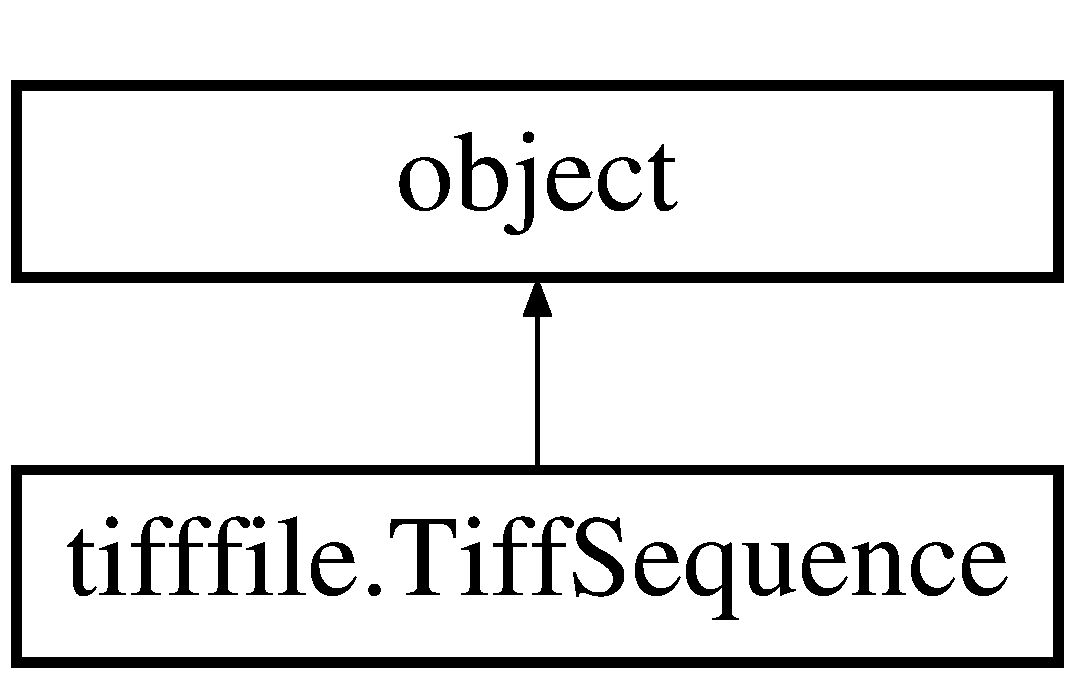
\includegraphics[height=2.000000cm]{classtifffile_1_1TiffSequence}
\end{center}
\end{figure}
\subsection*{Classes}
\begin{DoxyCompactItemize}
\item 
class \hyperlink{classtifffile_1_1TiffSequence_1_1ParseError}{Parse\-Error}
\end{DoxyCompactItemize}
\subsection*{Public Member Functions}
\begin{DoxyCompactItemize}
\item 
def \hyperlink{classtifffile_1_1TiffSequence_ad2a937998bb0fbb469fd45af3c5b9ee4}{\-\_\-\-\_\-init\-\_\-\-\_\-}
\item 
def \hyperlink{classtifffile_1_1TiffSequence_ab271e42b6b0a2d34069c16813b3c6396}{\-\_\-\-\_\-str\-\_\-\-\_\-}
\item 
\hypertarget{classtifffile_1_1TiffSequence_a1e84248e6ff24c50927c27ea3387ae20}{def {\bfseries \-\_\-\-\_\-len\-\_\-\-\_\-}}\label{classtifffile_1_1TiffSequence_a1e84248e6ff24c50927c27ea3387ae20}

\item 
\hypertarget{classtifffile_1_1TiffSequence_a22f8614649ba8ee39f28db15de453406}{def {\bfseries \-\_\-\-\_\-enter\-\_\-\-\_\-}}\label{classtifffile_1_1TiffSequence_a22f8614649ba8ee39f28db15de453406}

\item 
\hypertarget{classtifffile_1_1TiffSequence_a5af53397d4d20dc45a6afeafb7798103}{def {\bfseries \-\_\-\-\_\-exit\-\_\-\-\_\-}}\label{classtifffile_1_1TiffSequence_a5af53397d4d20dc45a6afeafb7798103}

\item 
\hypertarget{classtifffile_1_1TiffSequence_a66ea3eced1f21205b7fbc4632b7cf41a}{def {\bfseries close}}\label{classtifffile_1_1TiffSequence_a66ea3eced1f21205b7fbc4632b7cf41a}

\item 
def \hyperlink{classtifffile_1_1TiffSequence_a881cfef0cf4ae0deb1a3fd40b57ff38a}{asarray}
\end{DoxyCompactItemize}
\subsection*{Public Attributes}
\begin{DoxyCompactItemize}
\item 
\hypertarget{classtifffile_1_1TiffSequence_a734d6dfdbfbdc2d26c59e7413e9f78d4}{{\bfseries files}}\label{classtifffile_1_1TiffSequence_a734d6dfdbfbdc2d26c59e7413e9f78d4}

\item 
\hypertarget{classtifffile_1_1TiffSequence_a656d87f405cb67c7744470bef749c09d}{{\bfseries imread}}\label{classtifffile_1_1TiffSequence_a656d87f405cb67c7744470bef749c09d}

\item 
\hypertarget{classtifffile_1_1TiffSequence_a3ced8e56728d8dc84b95cd0e28dd8b29}{{\bfseries pattern}}\label{classtifffile_1_1TiffSequence_a3ced8e56728d8dc84b95cd0e28dd8b29}

\item 
\hypertarget{classtifffile_1_1TiffSequence_af80218f30eebb11ff3054df126b5e800}{{\bfseries axes}}\label{classtifffile_1_1TiffSequence_af80218f30eebb11ff3054df126b5e800}

\item 
\hypertarget{classtifffile_1_1TiffSequence_ae581d8715f29b3c6d03df21d139d68c9}{{\bfseries shape}}\label{classtifffile_1_1TiffSequence_ae581d8715f29b3c6d03df21d139d68c9}

\end{DoxyCompactItemize}


\subsection{Detailed Description}
\begin{DoxyVerb}Sequence of image files.

The data shape and dtype of all files must match.

Properties
----------
files : list
    List of file names.
shape : tuple
    Shape of image sequence.
axes : str
    Labels of axes in shape.

Examples
--------
>>> tifs = TiffSequence("test.oif.files/*.tif")
>>> tifs.shape, tifs.axes
((2, 100), 'CT')
>>> data = tifs.asarray()
>>> data.shape
(2, 100, 256, 256)\end{DoxyVerb}
 

\subsection{Constructor \& Destructor Documentation}
\hypertarget{classtifffile_1_1TiffSequence_ad2a937998bb0fbb469fd45af3c5b9ee4}{\index{tifffile\-::\-Tiff\-Sequence@{tifffile\-::\-Tiff\-Sequence}!\-\_\-\-\_\-init\-\_\-\-\_\-@{\-\_\-\-\_\-init\-\_\-\-\_\-}}
\index{\-\_\-\-\_\-init\-\_\-\-\_\-@{\-\_\-\-\_\-init\-\_\-\-\_\-}!tifffile::TiffSequence@{tifffile\-::\-Tiff\-Sequence}}
\subsubsection[{\-\_\-\-\_\-init\-\_\-\-\_\-}]{\setlength{\rightskip}{0pt plus 5cm}def tifffile.\-Tiff\-Sequence.\-\_\-\-\_\-init\-\_\-\-\_\- (
\begin{DoxyParamCaption}
\item[{}]{self, }
\item[{}]{files, }
\item[{}]{imread = {\ttfamily {\bf Tiff\-File}}, }
\item[{}]{pattern = {\ttfamily 'axes'}, }
\item[{}]{args, }
\item[{}]{kwargs}
\end{DoxyParamCaption}
)}}\label{classtifffile_1_1TiffSequence_ad2a937998bb0fbb469fd45af3c5b9ee4}
\begin{DoxyVerb}Initialize instance from multiple files.

Parameters
----------
files : str, or sequence of str
    Glob pattern or sequence of file names.
imread : function or class
    Image read function or class with asarray function returning numpy
    array from single file.
pattern : str
    Regular expression pattern that matches axes names and sequence
    indices in file names.
    By default this matches Olympus OIF and Leica TIFF series.\end{DoxyVerb}
 

\subsection{Member Function Documentation}
\hypertarget{classtifffile_1_1TiffSequence_ab271e42b6b0a2d34069c16813b3c6396}{\index{tifffile\-::\-Tiff\-Sequence@{tifffile\-::\-Tiff\-Sequence}!\-\_\-\-\_\-str\-\_\-\-\_\-@{\-\_\-\-\_\-str\-\_\-\-\_\-}}
\index{\-\_\-\-\_\-str\-\_\-\-\_\-@{\-\_\-\-\_\-str\-\_\-\-\_\-}!tifffile::TiffSequence@{tifffile\-::\-Tiff\-Sequence}}
\subsubsection[{\-\_\-\-\_\-str\-\_\-\-\_\-}]{\setlength{\rightskip}{0pt plus 5cm}def tifffile.\-Tiff\-Sequence.\-\_\-\-\_\-str\-\_\-\-\_\- (
\begin{DoxyParamCaption}
\item[{}]{self}
\end{DoxyParamCaption}
)}}\label{classtifffile_1_1TiffSequence_ab271e42b6b0a2d34069c16813b3c6396}
\begin{DoxyVerb}Return string with information about image sequence.\end{DoxyVerb}
 \hypertarget{classtifffile_1_1TiffSequence_a881cfef0cf4ae0deb1a3fd40b57ff38a}{\index{tifffile\-::\-Tiff\-Sequence@{tifffile\-::\-Tiff\-Sequence}!asarray@{asarray}}
\index{asarray@{asarray}!tifffile::TiffSequence@{tifffile\-::\-Tiff\-Sequence}}
\subsubsection[{asarray}]{\setlength{\rightskip}{0pt plus 5cm}def tifffile.\-Tiff\-Sequence.\-asarray (
\begin{DoxyParamCaption}
\item[{}]{self, }
\item[{}]{memmap = {\ttfamily False}, }
\item[{}]{args, }
\item[{}]{kwargs}
\end{DoxyParamCaption}
)}}\label{classtifffile_1_1TiffSequence_a881cfef0cf4ae0deb1a3fd40b57ff38a}
\begin{DoxyVerb}Read image data from all files and return as single numpy array.

If memmap is True, return an array stored in a binary file on disk.
The args and kwargs parameters are passed to the imread function.

Raise IndexError or ValueError if image shapes don't match.\end{DoxyVerb}
 

The documentation for this class was generated from the following file\-:\begin{DoxyCompactItemize}
\item 
/home/harold/workdir/atrex/\-Software/tifffile.\-py\end{DoxyCompactItemize}

\hypertarget{classtifffile_1_1TiffTag}{\section{tifffile.\-Tiff\-Tag Class Reference}
\label{classtifffile_1_1TiffTag}\index{tifffile.\-Tiff\-Tag@{tifffile.\-Tiff\-Tag}}
}
Inheritance diagram for tifffile.\-Tiff\-Tag\-:\begin{figure}[H]
\begin{center}
\leavevmode
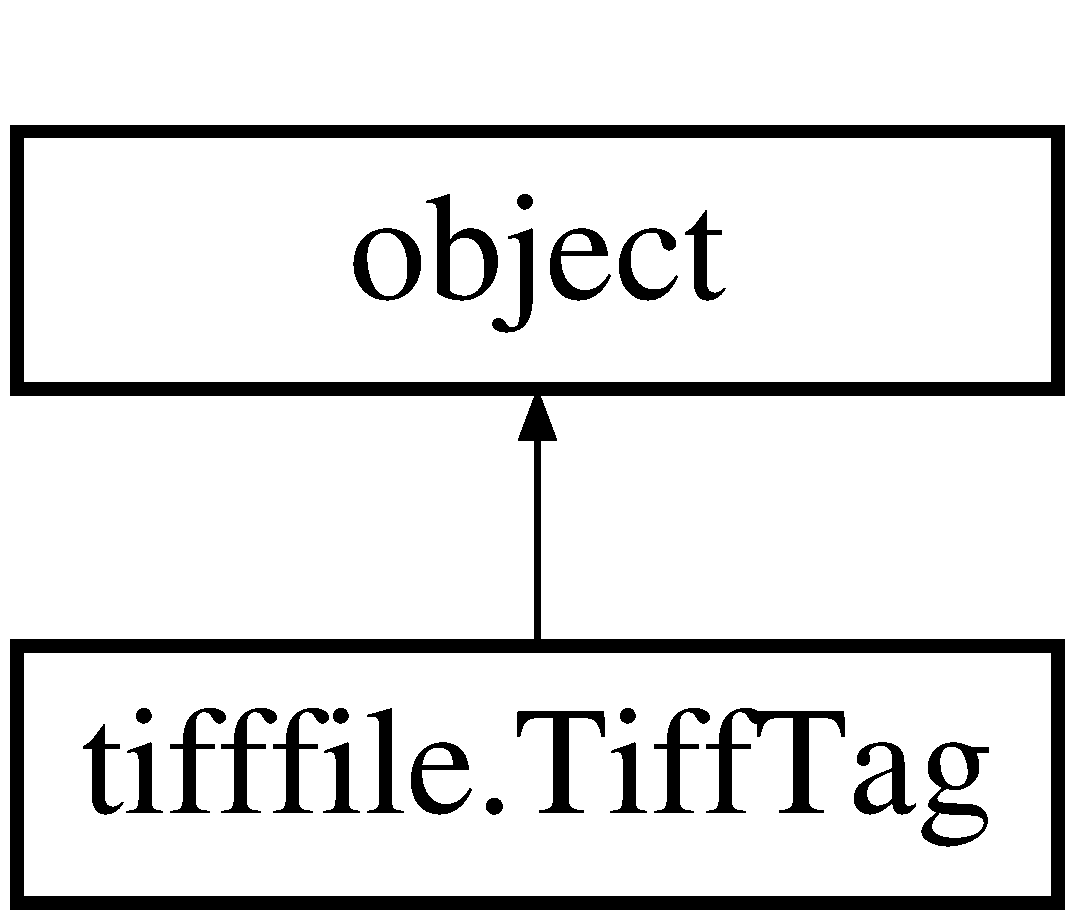
\includegraphics[height=2.000000cm]{classtifffile_1_1TiffTag}
\end{center}
\end{figure}
\subsection*{Classes}
\begin{DoxyCompactItemize}
\item 
class \hyperlink{classtifffile_1_1TiffTag_1_1Error}{Error}
\end{DoxyCompactItemize}
\subsection*{Public Member Functions}
\begin{DoxyCompactItemize}
\item 
def \hyperlink{classtifffile_1_1TiffTag_ace152e86d4dec367306b2aa8c966870a}{\-\_\-\-\_\-init\-\_\-\-\_\-}
\item 
def \hyperlink{classtifffile_1_1TiffTag_a6ee3a148b9b7d1233b30a011c0bbcecf}{as\-\_\-str}
\item 
def \hyperlink{classtifffile_1_1TiffTag_a3566254292688e9a17f1d71e1506c025}{\-\_\-\-\_\-str\-\_\-\-\_\-}
\end{DoxyCompactItemize}
\subsection*{Public Attributes}
\begin{DoxyCompactItemize}
\item 
\hypertarget{classtifffile_1_1TiffTag_a361450aec8540d6ae10e09a51cdd9bee}{{\bfseries code}}\label{classtifffile_1_1TiffTag_a361450aec8540d6ae10e09a51cdd9bee}

\item 
\hypertarget{classtifffile_1_1TiffTag_ac34a7b79c29ce864523c939668c5e4f7}{{\bfseries name}}\label{classtifffile_1_1TiffTag_ac34a7b79c29ce864523c939668c5e4f7}

\item 
\hypertarget{classtifffile_1_1TiffTag_a31e69f1557e2a9799fdddd2d461c4776}{{\bfseries dtype}}\label{classtifffile_1_1TiffTag_a31e69f1557e2a9799fdddd2d461c4776}

\item 
\hypertarget{classtifffile_1_1TiffTag_a20b7fd8e18b9c23e1e55a9bbdc00da3c}{{\bfseries count}}\label{classtifffile_1_1TiffTag_a20b7fd8e18b9c23e1e55a9bbdc00da3c}

\item 
\hypertarget{classtifffile_1_1TiffTag_a0578d5c23f06bde73d1728eb8da3461b}{{\bfseries value}}\label{classtifffile_1_1TiffTag_a0578d5c23f06bde73d1728eb8da3461b}

\item 
\hypertarget{classtifffile_1_1TiffTag_ac86aee4a1ef18fc194e4f0c753f74002}{{\bfseries value\-\_\-offset}}\label{classtifffile_1_1TiffTag_ac86aee4a1ef18fc194e4f0c753f74002}

\end{DoxyCompactItemize}


\subsection{Detailed Description}
\begin{DoxyVerb}A TIFF tag structure.

Attributes
----------
name : string
    Attribute name of tag.
code : int
    Decimal code of tag.
dtype : str
    Datatype of tag data. One of TIFF_DATA_TYPES.
count : int
    Number of values.
value : various types
    Tag data as Python object.
value_offset : int
    Location of value in file, if any.

All attributes are read-only.\end{DoxyVerb}
 

\subsection{Constructor \& Destructor Documentation}
\hypertarget{classtifffile_1_1TiffTag_ace152e86d4dec367306b2aa8c966870a}{\index{tifffile\-::\-Tiff\-Tag@{tifffile\-::\-Tiff\-Tag}!\-\_\-\-\_\-init\-\_\-\-\_\-@{\-\_\-\-\_\-init\-\_\-\-\_\-}}
\index{\-\_\-\-\_\-init\-\_\-\-\_\-@{\-\_\-\-\_\-init\-\_\-\-\_\-}!tifffile::TiffTag@{tifffile\-::\-Tiff\-Tag}}
\subsubsection[{\-\_\-\-\_\-init\-\_\-\-\_\-}]{\setlength{\rightskip}{0pt plus 5cm}def tifffile.\-Tiff\-Tag.\-\_\-\-\_\-init\-\_\-\-\_\- (
\begin{DoxyParamCaption}
\item[{}]{self, }
\item[{}]{arg, }
\item[{}]{kwargs}
\end{DoxyParamCaption}
)}}\label{classtifffile_1_1TiffTag_ace152e86d4dec367306b2aa8c966870a}
\begin{DoxyVerb}Initialize instance from file or arguments.\end{DoxyVerb}
 

\subsection{Member Function Documentation}
\hypertarget{classtifffile_1_1TiffTag_a3566254292688e9a17f1d71e1506c025}{\index{tifffile\-::\-Tiff\-Tag@{tifffile\-::\-Tiff\-Tag}!\-\_\-\-\_\-str\-\_\-\-\_\-@{\-\_\-\-\_\-str\-\_\-\-\_\-}}
\index{\-\_\-\-\_\-str\-\_\-\-\_\-@{\-\_\-\-\_\-str\-\_\-\-\_\-}!tifffile::TiffTag@{tifffile\-::\-Tiff\-Tag}}
\subsubsection[{\-\_\-\-\_\-str\-\_\-\-\_\-}]{\setlength{\rightskip}{0pt plus 5cm}def tifffile.\-Tiff\-Tag.\-\_\-\-\_\-str\-\_\-\-\_\- (
\begin{DoxyParamCaption}
\item[{}]{self}
\end{DoxyParamCaption}
)}}\label{classtifffile_1_1TiffTag_a3566254292688e9a17f1d71e1506c025}
\begin{DoxyVerb}Return string containing information about tag.\end{DoxyVerb}
 \hypertarget{classtifffile_1_1TiffTag_a6ee3a148b9b7d1233b30a011c0bbcecf}{\index{tifffile\-::\-Tiff\-Tag@{tifffile\-::\-Tiff\-Tag}!as\-\_\-str@{as\-\_\-str}}
\index{as\-\_\-str@{as\-\_\-str}!tifffile::TiffTag@{tifffile\-::\-Tiff\-Tag}}
\subsubsection[{as\-\_\-str}]{\setlength{\rightskip}{0pt plus 5cm}def tifffile.\-Tiff\-Tag.\-as\-\_\-str (
\begin{DoxyParamCaption}
\item[{}]{self}
\end{DoxyParamCaption}
)}}\label{classtifffile_1_1TiffTag_a6ee3a148b9b7d1233b30a011c0bbcecf}
\begin{DoxyVerb}Return value as human readable string.\end{DoxyVerb}
 

The documentation for this class was generated from the following file\-:\begin{DoxyCompactItemize}
\item 
/home/harold/workdir/atrex/\-Software/tifffile.\-py\end{DoxyCompactItemize}

\hypertarget{classtifffile_1_1TiffTags}{\section{tifffile.\-Tiff\-Tags Class Reference}
\label{classtifffile_1_1TiffTags}\index{tifffile.\-Tiff\-Tags@{tifffile.\-Tiff\-Tags}}
}
Inheritance diagram for tifffile.\-Tiff\-Tags\-:\begin{figure}[H]
\begin{center}
\leavevmode
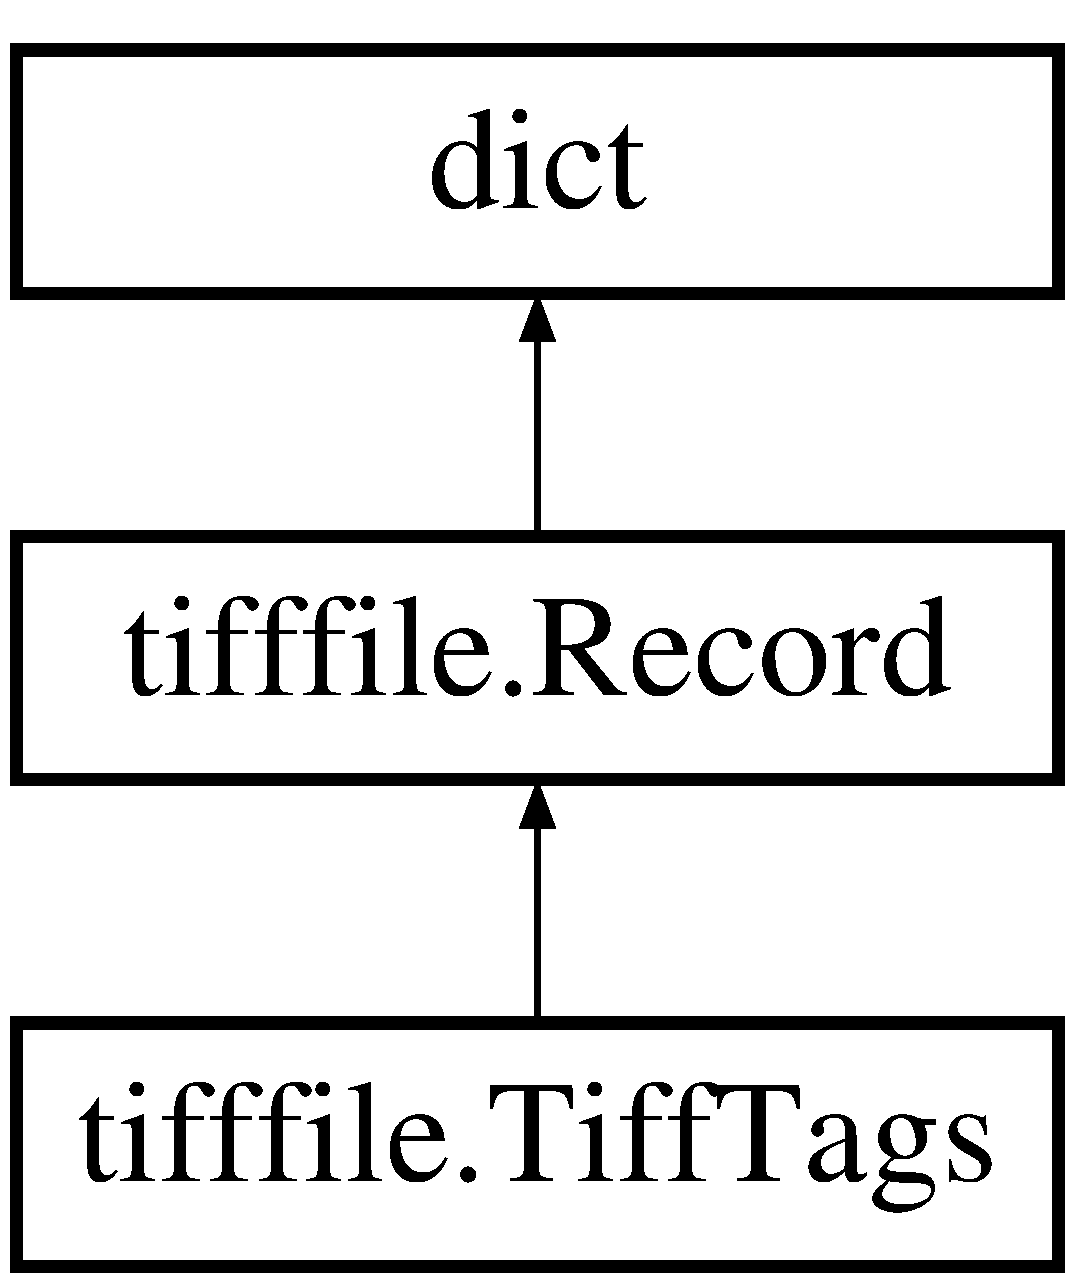
\includegraphics[height=3.000000cm]{classtifffile_1_1TiffTags}
\end{center}
\end{figure}
\subsection*{Public Member Functions}
\begin{DoxyCompactItemize}
\item 
def \hyperlink{classtifffile_1_1TiffTags_a68afbd2339eb5c7a6c02eea60a16ce65}{\-\_\-\-\_\-str\-\_\-\-\_\-}
\end{DoxyCompactItemize}


\subsection{Detailed Description}
\begin{DoxyVerb}Dictionary of TiffTag with attribute access.\end{DoxyVerb}
 

\subsection{Member Function Documentation}
\hypertarget{classtifffile_1_1TiffTags_a68afbd2339eb5c7a6c02eea60a16ce65}{\index{tifffile\-::\-Tiff\-Tags@{tifffile\-::\-Tiff\-Tags}!\-\_\-\-\_\-str\-\_\-\-\_\-@{\-\_\-\-\_\-str\-\_\-\-\_\-}}
\index{\-\_\-\-\_\-str\-\_\-\-\_\-@{\-\_\-\-\_\-str\-\_\-\-\_\-}!tifffile::TiffTags@{tifffile\-::\-Tiff\-Tags}}
\subsubsection[{\-\_\-\-\_\-str\-\_\-\-\_\-}]{\setlength{\rightskip}{0pt plus 5cm}def tifffile.\-Tiff\-Tags.\-\_\-\-\_\-str\-\_\-\-\_\- (
\begin{DoxyParamCaption}
\item[{}]{self}
\end{DoxyParamCaption}
)}}\label{classtifffile_1_1TiffTags_a68afbd2339eb5c7a6c02eea60a16ce65}
\begin{DoxyVerb}Return string with information about all tags.\end{DoxyVerb}
 

The documentation for this class was generated from the following file\-:\begin{DoxyCompactItemize}
\item 
/home/harold/workdir/atrex/\-Software/tifffile.\-py\end{DoxyCompactItemize}

\hypertarget{classtifffile_1_1TiffWriter}{\section{tifffile.\-Tiff\-Writer Class Reference}
\label{classtifffile_1_1TiffWriter}\index{tifffile.\-Tiff\-Writer@{tifffile.\-Tiff\-Writer}}
}
Inheritance diagram for tifffile.\-Tiff\-Writer\-:\begin{figure}[H]
\begin{center}
\leavevmode
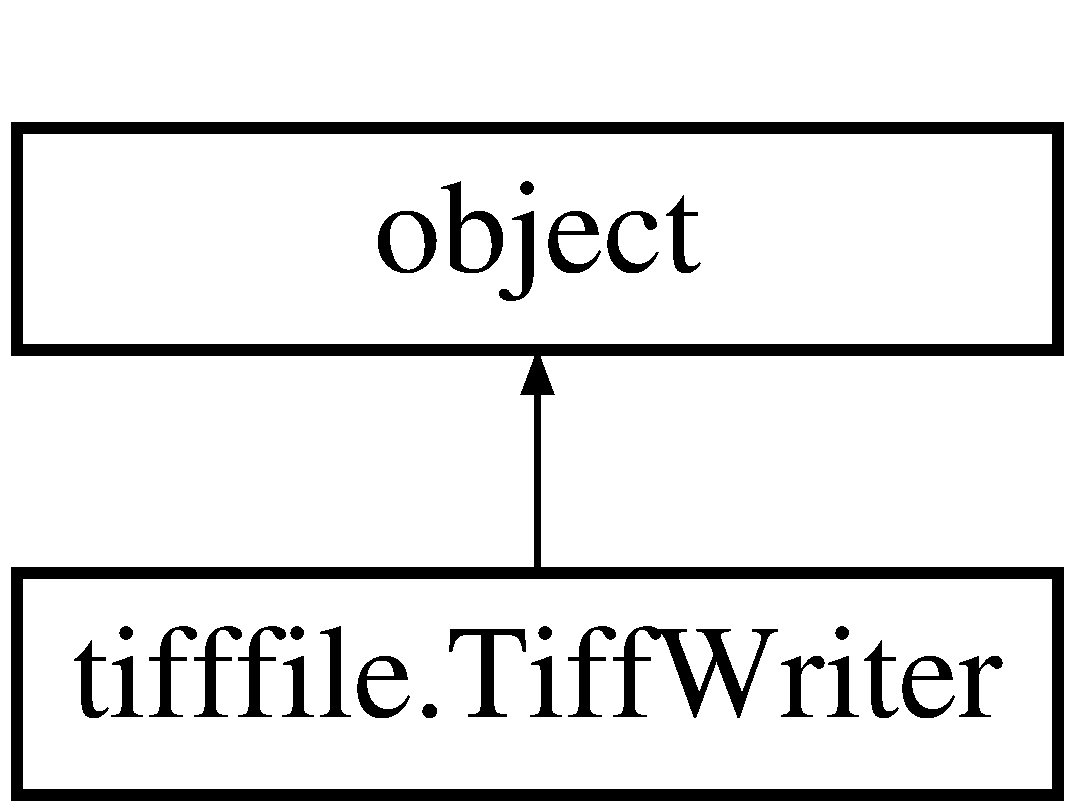
\includegraphics[height=2.000000cm]{classtifffile_1_1TiffWriter}
\end{center}
\end{figure}
\subsection*{Public Member Functions}
\begin{DoxyCompactItemize}
\item 
def \hyperlink{classtifffile_1_1TiffWriter_af9fb37461e229375ed0b7c7aa56fcf2a}{\-\_\-\-\_\-init\-\_\-\-\_\-}
\item 
def \hyperlink{classtifffile_1_1TiffWriter_a7879708dbcc972bda2148374bddbec0d}{save}
\item 
\hypertarget{classtifffile_1_1TiffWriter_a579dd794187e65874987990058ba70aa}{def {\bfseries close}}\label{classtifffile_1_1TiffWriter_a579dd794187e65874987990058ba70aa}

\item 
\hypertarget{classtifffile_1_1TiffWriter_aeb1a99b0e609acf41b4a96029397724d}{def {\bfseries \-\_\-\-\_\-enter\-\_\-\-\_\-}}\label{classtifffile_1_1TiffWriter_aeb1a99b0e609acf41b4a96029397724d}

\item 
\hypertarget{classtifffile_1_1TiffWriter_a9a746e2cea3adaab40913a74fb56ca60}{def {\bfseries \-\_\-\-\_\-exit\-\_\-\-\_\-}}\label{classtifffile_1_1TiffWriter_a9a746e2cea3adaab40913a74fb56ca60}

\end{DoxyCompactItemize}
\subsection*{Static Public Attributes}
\begin{DoxyCompactItemize}
\item 
dictionary {\bfseries T\-Y\-P\-E\-S}
\item 
dictionary {\bfseries T\-A\-G\-S}
\end{DoxyCompactItemize}


\subsection{Detailed Description}
\begin{DoxyVerb}Write image data to TIFF file.

TiffWriter instances must be closed using the close method, which is
automatically called when using the 'with' statement.

Examples
--------
>>> data = numpy.random.rand(2, 5, 3, 301, 219)
>>> with TiffWriter('temp.tif', bigtiff=True) as tif:
...     for i in range(data.shape[0]):
...         tif.save(data[i], compress=6)\end{DoxyVerb}
 

\subsection{Constructor \& Destructor Documentation}
\hypertarget{classtifffile_1_1TiffWriter_af9fb37461e229375ed0b7c7aa56fcf2a}{\index{tifffile\-::\-Tiff\-Writer@{tifffile\-::\-Tiff\-Writer}!\-\_\-\-\_\-init\-\_\-\-\_\-@{\-\_\-\-\_\-init\-\_\-\-\_\-}}
\index{\-\_\-\-\_\-init\-\_\-\-\_\-@{\-\_\-\-\_\-init\-\_\-\-\_\-}!tifffile::TiffWriter@{tifffile\-::\-Tiff\-Writer}}
\subsubsection[{\-\_\-\-\_\-init\-\_\-\-\_\-}]{\setlength{\rightskip}{0pt plus 5cm}def tifffile.\-Tiff\-Writer.\-\_\-\-\_\-init\-\_\-\-\_\- (
\begin{DoxyParamCaption}
\item[{}]{self, }
\item[{}]{filename, }
\item[{}]{bigtiff = {\ttfamily False}, }
\item[{}]{byteorder = {\ttfamily None}, }
\item[{}]{software = {\ttfamily 'tifffile.py'}}
\end{DoxyParamCaption}
)}}\label{classtifffile_1_1TiffWriter_af9fb37461e229375ed0b7c7aa56fcf2a}
\begin{DoxyVerb}Create a new TIFF file for writing.

Use bigtiff=True when creating files greater than 2 GB.

Parameters
----------
filename : str
    Name of file to write.
bigtiff : bool
    If True, the BigTIFF format is used.
byteorder : {'<', '>'}
    The endianness of the data in the file.
    By default this is the system's native byte order.
software : str
    Name of the software used to create the image.
    Saved with the first page only.\end{DoxyVerb}
 

\subsection{Member Function Documentation}
\hypertarget{classtifffile_1_1TiffWriter_a7879708dbcc972bda2148374bddbec0d}{\index{tifffile\-::\-Tiff\-Writer@{tifffile\-::\-Tiff\-Writer}!save@{save}}
\index{save@{save}!tifffile::TiffWriter@{tifffile\-::\-Tiff\-Writer}}
\subsubsection[{save}]{\setlength{\rightskip}{0pt plus 5cm}def tifffile.\-Tiff\-Writer.\-save (
\begin{DoxyParamCaption}
\item[{}]{self, }
\item[{}]{data, }
\item[{}]{photometric = {\ttfamily None}, }
\item[{}]{planarconfig = {\ttfamily None}, }
\item[{}]{resolution = {\ttfamily None}, }
\item[{}]{description = {\ttfamily None}, }
\item[{}]{volume = {\ttfamily False}, }
\item[{}]{writeshape = {\ttfamily False}, }
\item[{}]{compress = {\ttfamily 0}, }
\item[{}]{extratags = {\ttfamily ()}}
\end{DoxyParamCaption}
)}}\label{classtifffile_1_1TiffWriter_a7879708dbcc972bda2148374bddbec0d}
\begin{DoxyVerb}Write image data to TIFF file.

Image data are written in one stripe per plane.
Dimensions larger than 2 to 4 (depending on photometric mode, planar
configuration, and SGI mode) are flattened and saved as separate pages.
The 'sample_format' and 'bits_per_sample' TIFF tags are derived from
the data type.

Parameters
----------
data : array_like
    Input image. The last dimensions are assumed to be image depth,
    height, width, and samples.
photometric : {'minisblack', 'miniswhite', 'rgb'}
    The color space of the image data.
    By default this setting is inferred from the data shape.
planarconfig : {'contig', 'planar'}
    Specifies if samples are stored contiguous or in separate planes.
    By default this setting is inferred from the data shape.
    'contig': last dimension contains samples.
    'planar': third last dimension contains samples.
resolution : (float, float) or ((int, int), (int, int))
    X and Y resolution in dots per inch as float or rational numbers.
description : str
    The subject of the image. Saved with the first page only.
compress : int
    Values from 0 to 9 controlling the level of zlib compression.
    If 0, data are written uncompressed (default).
volume : bool
    If True, volume data are stored in one tile (if applicable) using
    the SGI image_depth and tile_depth tags.
    Image width and depth must be multiple of 16.
    Few software can read this format, e.g. MeVisLab.
writeshape : bool
    If True, write the data shape to the image_description tag
    if necessary and no other description is given.
extratags: sequence of tuples
    Additional tags as [(code, dtype, count, value, writeonce)].

    code : int
The TIFF tag Id.
    dtype : str
Data type of items in 'value' in Python struct format.
One of B, s, H, I, 2I, b, h, i, f, d, Q, or q.
    count : int
Number of data values. Not used for string values.
    value : sequence
'Count' values compatible with 'dtype'.
    writeonce : bool
If True, the tag is written to the first page only.\end{DoxyVerb}
 

\subsection{Member Data Documentation}
\hypertarget{classtifffile_1_1TiffWriter_a59306b1d4123917f8ef19b622932be69}{\index{tifffile\-::\-Tiff\-Writer@{tifffile\-::\-Tiff\-Writer}!T\-A\-G\-S@{T\-A\-G\-S}}
\index{T\-A\-G\-S@{T\-A\-G\-S}!tifffile::TiffWriter@{tifffile\-::\-Tiff\-Writer}}
\subsubsection[{T\-A\-G\-S}]{\setlength{\rightskip}{0pt plus 5cm}dictionary tifffile.\-Tiff\-Writer.\-T\-A\-G\-S\hspace{0.3cm}{\ttfamily [static]}}}\label{classtifffile_1_1TiffWriter_a59306b1d4123917f8ef19b622932be69}
{\bfseries Initial value\-:}
\begin{DoxyCode}
1 = \{
2         \textcolor{stringliteral}{'new\_subfile\_type'}: 254, \textcolor{stringliteral}{'subfile\_type'}: 255,
3         \textcolor{stringliteral}{'image\_width'}: 256, \textcolor{stringliteral}{'image\_length'}: 257, \textcolor{stringliteral}{'bits\_per\_sample'}: 258,
4         \textcolor{stringliteral}{'compression'}: 259, \textcolor{stringliteral}{'photometric'}: 262, \textcolor{stringliteral}{'fill\_order'}: 266,
5         \textcolor{stringliteral}{'document\_name'}: 269, \textcolor{stringliteral}{'image\_description'}: 270, \textcolor{stringliteral}{'strip\_offsets'}: 273,
6         \textcolor{stringliteral}{'orientation'}: 274, \textcolor{stringliteral}{'samples\_per\_pixel'}: 277, \textcolor{stringliteral}{'rows\_per\_strip'}: 278,
7         \textcolor{stringliteral}{'strip\_byte\_counts'}: 279, \textcolor{stringliteral}{'x\_resolution'}: 282, \textcolor{stringliteral}{'y\_resolution'}: 283,
8         \textcolor{stringliteral}{'planar\_configuration'}: 284, \textcolor{stringliteral}{'page\_name'}: 285, \textcolor{stringliteral}{'resolution\_unit'}: 296,
9         \textcolor{stringliteral}{'software'}: 305, \textcolor{stringliteral}{'datetime'}: 306, \textcolor{stringliteral}{'predictor'}: 317, \textcolor{stringliteral}{'color\_map'}: 320,
10         \textcolor{stringliteral}{'tile\_width'}: 322, \textcolor{stringliteral}{'tile\_length'}: 323, \textcolor{stringliteral}{'tile\_offsets'}: 324,
11         \textcolor{stringliteral}{'tile\_byte\_counts'}: 325, \textcolor{stringliteral}{'extra\_samples'}: 338, \textcolor{stringliteral}{'sample\_format'}: 339,
12         \textcolor{stringliteral}{'image\_depth'}: 32997, \textcolor{stringliteral}{'tile\_depth'}: 32998\}
\end{DoxyCode}
\hypertarget{classtifffile_1_1TiffWriter_aae9c1bc9345c95fe80d2d31188e6e23d}{\index{tifffile\-::\-Tiff\-Writer@{tifffile\-::\-Tiff\-Writer}!T\-Y\-P\-E\-S@{T\-Y\-P\-E\-S}}
\index{T\-Y\-P\-E\-S@{T\-Y\-P\-E\-S}!tifffile::TiffWriter@{tifffile\-::\-Tiff\-Writer}}
\subsubsection[{T\-Y\-P\-E\-S}]{\setlength{\rightskip}{0pt plus 5cm}dictionary tifffile.\-Tiff\-Writer.\-T\-Y\-P\-E\-S\hspace{0.3cm}{\ttfamily [static]}}}\label{classtifffile_1_1TiffWriter_aae9c1bc9345c95fe80d2d31188e6e23d}
{\bfseries Initial value\-:}
\begin{DoxyCode}
1 = \{\textcolor{stringliteral}{'B'}: 1, \textcolor{stringliteral}{'s'}: 2, \textcolor{stringliteral}{'H'}: 3, \textcolor{stringliteral}{'I'}: 4, \textcolor{stringliteral}{'2I'}: 5, \textcolor{stringliteral}{'b'}: 6,
2              \textcolor{stringliteral}{'h'}: 8, \textcolor{stringliteral}{'i'}: 9, \textcolor{stringliteral}{'f'}: 11, \textcolor{stringliteral}{'d'}: 12, \textcolor{stringliteral}{'Q'}: 16, \textcolor{stringliteral}{'q'}: 17\}
\end{DoxyCode}


The documentation for this class was generated from the following file\-:\begin{DoxyCompactItemize}
\item 
/home/harold/workdir/atrex/\-Software/tifffile.\-py\end{DoxyCompactItemize}

%--- End generated contents ---

% Index
\newpage
\phantomsection
\addcontentsline{toc}{part}{Index}
\printindex

\end{document}
